\documentclass[a4paper,12pt]{article}
\usepackage{amsmath,amsfonts,amsthm,amscd,amssymb,latexsym}%,eufrak}
%%%%%%%%%%%%%
\usepackage{caption}
\usepackage{subcaption}
\usepackage{enumerate,graphicx,psfrag}%,subfigure}%,jchangebar,oldgerm}
\usepackage[mathscr]{eucal}
\usepackage[usenames]{color}
\usepackage{url}
\usepackage[shortlabels]{enumitem}
\usepackage{comment}
%\usepackage[utf8]{inputenc}
\usepackage[T1]{fontenc}
\usepackage{showkeys}
%%%%%%%%%
\sloppy
%%%%%%%%%%%%%%%%%%%%%%%
\title{The subgroup membership problem
}
\author{Andrew J. Duncan, Elizaveta Frenkel}

\renewcommand{\a}{\alpha }
\renewcommand{\b}{\beta }
\newcommand{\G}{\Gamma }
\newcommand{\g}{\gamma }
\newcommand{\D}{\Delta }
\renewcommand{\d}{\delta }
%\def\vd{\vardelta}
\newcommand{\ep}{\epsilon }
\newcommand{\e}{\varepsilon }
\newcommand{\z}{\zeta }
%\eta
\renewcommand{\th}{\theta }
\newcommand{\T}{\Theta }
\renewcommand{\i}{\iota }
\renewcommand{\k}{\kappa }
\renewcommand{\l}{\lambda }
\renewcommand{\L}{\Lambda }
%\mu
%\nu
%\xi
%omicron
%\pi
\renewcommand{\r}{\rho }
\newcommand{\s}{\sigma }
\renewcommand{\S}{\Sigma }
\renewcommand{\t}{\tau }
\newcommand{\up}{\upsilon }
\newcommand{\U}{\Upsilon }
%\phi
\newcommand{\x}{\chi }
%\psi
\newcommand{\W}{\Omega }
\newcommand{\w}{\omega }
%%%%%%%%%%%%%%%%%%%%%%%%%%%%%%%
%%%%%%%%%%%%%%%%%%%%%%%%%%%%%
\newcommand{\pd}{\partial}
\newcommand{\wht}{\widehat}
%\newcommand{\cC}{{\mathcal C}}
%\newcommand{\cdim}{\texttt{cdim}}
\newcommand{\fC}{{\textswab C}}
\newenvironment{ef}{\noindent\color{blue} \bf EF: }{}
%
\newcommand{\cA}{{\cal{A}}}
\newcommand{\cD}{{\cal{D}}}
\newcommand{\cF}{{\cal{F}}}
\newcommand{\cH}{{\cal{H}}}
\newcommand{\cJ}{{\cal{J}}}
\newcommand{\cK}{{\cal{K}}}
\newcommand{\cP}{{\cal{P}}}
\newcommand{\cQ}{{\cal{Q}}}
\newcommand{\cR}{{\cal{R}}}
\newcommand{\cS}{{\cal{S}}}
\newcommand{\cV}{{\cal{V}}}
\newcommand{\cW}{{\cal{W}}}
%\newcommand{\GG}{\ensuremath{\mathbb{G}}}
\newcommand{\pp}{\mathbf{p}}
%%%%%%%%%%%%%%%%%%%%%%%%%%%%%%
\newcommand{\nul}{\emptyset }
\newcommand{\vim}{\nu\textrm{-im}}
%%%%%%%%%%%%%%%%%%%%%%%%%%%%%%
\newtheorem{theorem}{Theorem}[section]
\newtheorem{lemma}[theorem]{Lemma}
\newtheorem{corollary}[theorem]{Corollary}
\newtheorem{proposition}[theorem]{Proposition}
\newtheorem{axiom}[theorem]{Axiom}
\newtheorem{definition}[theorem]{Definition}
\newtheorem*{defn*}{Definition}
\newtheorem{conjecture}[theorem]{Conjecture}
%cvs -d :pserver:najd2@cvs.mas.ncl.ac.uk:/CVS/najd2
\newtheorem{exam}[theorem]{Example}
%\newtheorem{comment}[theorem]{Comment}
%
%
\newenvironment{example}{\begin{exam} \rm}{\end{exam}}
%
%
%
\newtheorem{remk}[theorem]{Remark}
\newenvironment{remark}{\begin{remk} \rm}{\end{remk}}
%
%%%%%%%%%%%%
\numberwithin{equation}{section}
\numberwithin{figure}{section}
%%%%%%%%%%%%%%%%%%%%
\newcommand{\Loop}{\operatorname{Loop}}
\newcommand{\Iso}{\operatorname{Isom}}
\newcommand{\Aut}{\operatorname{Aut}}
%%%%%%%%%%%%%%%%%%%
\renewcommand{\AA}{\ensuremath{\mathbb{A}}}
\newcommand{\ZZ}{\ensuremath{\mathbb{Z}}}
\newcommand{\QQ}{\ensuremath{\mathbb{Q}}}
\newcommand{\RR}{\ensuremath{\mathbb{R}}}
\newcommand{\NN}{\ensuremath{\mathbb{N}}}
\newcommand{\CC}{\ensuremath{\mathbb{C}}}
\newcommand{\FF}{\ensuremath{\mathbb{F}}}
%\renewcommand{\ker}{\verb"Ker"}
\newcommand{\cC}{\mathcal{C}}
\renewcommand{\cF}{\mathcal{F}}
\newcommand{\cO}{\mathcal{O}}
\renewcommand{\cS}{\mathcal{S}}
\newcommand{\la}{\langle}
\newcommand{\ra}{\rangle}
%\newcommand{\BA}{\ensuremath{\mathbb{A}}}
%%%%%%%%%%%%%%%%%%%%%%%%%%%%%%%%%%%%%%
\newcommand{\maps}{\rightarrow}
\newcommand{\ov}[1]{\overline{#1}}
\newcommand{\bs}{\backslash}
%%%%%%%%%%%%%%%%%%%%%%%%%%%%%%%
\newcommand{\be}{\begin{enumerate}}
\newcommand{\ee}{\end{enumerate}}
\newcommand{\bd}{\begin{description}}
\newcommand{\ed}{\end{description}}
\newcommand{\biz}{\begin{itemize}}
\newcommand{\eiz}{\end{itemize}}
%%%%%%%%%%%%%%%%%%%%%%%%%%%%%%%%%%%
%
\newenvironment{ajd1}{\noindent\color{red} AJD }{}
\newcommand{\ajd}[1]{\begin{ajd1} #1 \end{ajd1}}
%
%\includecomment{comp}% to see environment comp
\excludecomment{comp}% to hide environment comp
%
\begin{document}
\maketitle

\begin{abstract}
Stallings folding theory is modified, using double coset representatives, and to applied
to the study of subgroups of  amalgamated
products of finite rank free groups. As an application the
 subgroup membership
problem for such groups is shown to be decidable. An algorithm for this
problem is constructed and its complexity is analysed.
 \end{abstract}



\section{Introduction}\label{se:global_intro}

Stallings introduced his technique of subgroup foldings in
\cite{stallings83} where he applied it to investigate subgroups of
free groups. In \cite{stallings88} Stallings extended ideas of
foldings to non-free actions of groups on graphs and trees. In the following
years these ideas were widely generalised, in several
directions,  and used to solve a variety of  problems in
combinatorial group theory: see for example
\cite{befe,BoWei,KM02,SilvaWeil08}.
In this paper we consider  subgroups
of free products with amalgamation of free groups of finite rank, using
a language of normal forms based on double coset representatives.  We
extend the theory  of Stallings foldings to this setting and use it to construct an
explicit algorithm for the subgroup membership problem.

Let $G = <X|R>$ be a finitely generated group.
The \emph{subgroup  membership problem}, for  fixed subgroup $K$ of $G$,
is to decide whether or not a given  word $w$ in $\FF(X)$ represents an element of  the subgroup $K$.
The \emph{uniform} subgroup membership problem for $G$ is to decide,
given a finite subset $P=\{w,k_1,\ldots ,k_s\}$ of elements of $\FF(X)$,
for some $s\ge 0$,
whether or not $w$ represents an element of  the subgroup $K$ of $G$
generated by $Y=P\backslash\{w\}$.
The  subgroup membership problem for $K$ in $G$ is said to be
\emph{solvable} if there is an algorithm which, on input $w\in \FF(X)$,
outputs ``yes'' if and only if $w$ does represent an element of $K$.
Similarly, the uniform subgroup membership problem for $G$ is \emph{solvable}
if there exists an algorithm which, on input $P$, outputs ``yes'' if
and only if $w$ represents an element of $K$.

Associated to the subgroup membership problem for the subgroup $K$ of the group $G$,
generated by a finite set $Y=\{k_1,\ldots, k_s\}$, as
above, is the \emph{subgroup membership search problem}:
given an element $w\in \FF(X)$ such
that $w$ represents an element of $K$, find a sequence of pairs
$(k_{i_j},\e_j)$, $m=1,\ldots ,t$, for some $t\in \NN$, $k_{i_j}\in \{k_1,\ldots, k_s\}$
and $\e_j=\pm 1$,  such that
$w=k_{i_1}^{\e_1}\cdots k_{i_t}^{\e_t}$ in the group $G$.  The subgroup $K$
is said to have
\emph{solvable  membership search problem} if there is an algorithm which, on input
a word $w$ in $\FF(X)$ representing an element of $K$, will output such
 a sequence. The  \emph{uniform membership search problem} and
its solvability,
for a group $G$, are
defined
in the obvious way.


If $\cV$ is a class of groups and there exists an algorithm to
solve the uniform membership (search) problem for any element of $\cV$ then
we say that $\cV$ has solvable uniform  (search) membership problem.

\begin{theorem}\label{thm:membership}
Let $F_1$ and $F_2$ be finite rank free groups and let $H_1$ and $H_2$
be finitely generated subgroups of $F_1$ and $F_2$, respectively, such
that $H_1$ is isomorphic to $H_2$. Let $G=F_1 \ast_{H_1=H_2} F_2$.
Let $\cF$ be the class of free products with amalgamation, where
factors are free of finite rank, and the amalgamated subgroups are
finitely generated.
Then
\be
\item\label{it:membership}
$G$ has solvable membership problem,
\item \label{it:uni-membership}
$G$ has solvable uniform  membership problem and
\item\label{it:class-uni-membership}
$\cF$ has solvable uniform  membership problem.
\ee
Moreover the same conclusions hold for the search versions of each of these
problems.
\end{theorem}


``Free group constructions'', in particular, free products of groups,
with or without amalgamation, $HNN$-extensions
 and, more generally, fundamental groups
of graphs of groups constitute a subject of special significance in
group theory, from many points of view. Initial results in this area,
related to the solvability of membership problem,  due to Mihailova (see
\cite{mi59,mi68}), show that the membership problem is
decidable in the free product of groups $A$ and $B$ if it is decidable
in both factors. Another famous result of
Mihailova \cite{mi58}  provides an important counter-example:
 namely,  a finitely generated
subgroup of a direct product of two free groups of rank two with
unsolvable membership problem.  This direct
product can in fact be considered as a sequence of two $HNN$-extensions
of rank two free group. On the other hand, another classical
result \cite[Proposition 2.21]{LS} shows that a free group of finite rank has
solvable (uniform)
membership problem. Thus,  even innocent group
constructions can dramatically affect solvability of the membership problem.

The membership problem for free products with amalgamation and
$HNN$-extensions was studied by Bezverkhnii in papers
\cite{bez81,bez86,bez90,bez91}, using  combinatorial
techniques and standard normal forms for  amalgamated products of
groups. Our approach is, first of all, more geometric, and since
we have an eye on a generalisation of results to other free
constructions, we have been led to introduce alternative normal forms
 appropriate to
study of these constructions.

Another significant step in development of the theory of foldings for
free constructions
 was taken by Kapovich, Miasnikov and Weidmann
\cite{KMW03}, where the authors investigated the uniform membership
problem for fundamental groups of graphs of groups, under certain
assumptions on both vertex and edge groups. In particular, they
showed that, in the case where all vertex groups are either locally
quasiconvex word hyperbolic or polycyclic-by-finite, and all edge
groups are polycyclic-by-finite; the uniform membership problem for the
fundamental group of the graph of groups is solvable.

As mentioned above, we  introduce a  geometric
technique, which relies on Stallings foldings and
normal forms based on double cosets, for elements of amalgamated products of
groups.

Now, a few words on the structure of the paper. In Section
\ref{sec:dcforms} we introduce double coset repreesentatives for
elements of free groups, with respect to a fixed subgroup,
%These representatives are used to define double coset normal forms
%We show that these representatives
%are unique
and
  describe an explicit procedure
 for their construction.
These representatives are used to define unique double coset normal forms
for elements of
amalgamated products of finite rank free groups in Section  \ref{sec:foldings}, which
 is the heart of the paper. For a subgroup $K$ of such an amalgam, we
describe a generalised folding process, which begins with the flower automaton
of $K$, over an extended alphabet, and results in
a ``double coset graph'' for $K$, which  recognises
precisely the  normal forms of elements of $K$.

In Section \ref{sec:TC} we estimate the time complexity of
algorithms described in the previous parts of the paper. In
particular, we illustrate how quickly the  preparatory
work in construction of  double coset normal forms of generators
for $K$  can be carried out; we calculate  the complexity of the process of
modification of
components of the flower automaton of $K$, and of the reassembly process required to
produce the double coset graph.

The authors are grateful to Vladimir Remeslennikov for suggesting the use of double
cosets and
for helpful
discussions,  and to Christian Perfect who gave invaluable help with programming.


\begin{comment}
\section{Double coset normal form}\label{sec:intro}
Based on notes copied (laboriously) from Christian's page
\url{
http://checkmyworking.com/misc/writemaths/?doublecoset
}

$F_1$, $F_2$ free groups (finitely generated by $X_1$
and $X_2$, respectively).

Let $H_1 \leq F_1$, $H_2 \leq F_2$ such that
there exists an isomorphism $\phi: H_1 \rightarrow H_2$.

i.e. we have finite bases $\{h_1, \ldots, h_m \}$  for $H_1$ and
$\{h_1', \ldots, h_m'\}$ for $H_2$.

Consider the free group $\FF(Z)$, generated by $Z=\{z_1, \ldots, z_m\}$,
and the maps $\phi_1$ and $\phi_2$ such that
$\phi_1(z_i)=h_i(X_1)  $ and  $\phi_2(z_i)=h^\prime_i(X_2)$, $i=1,\ldots ,m$.
Thus $\phi_i$ extends to an isomorphism of $\FF(Z)$ to $H_i$. We choose
the $\phi_i$ so that $\phi=\phi_2\phi_1^{-1}$.

Let ${G = F_1 \underset{H_1=H_2}{\ast} F_2}$, the group with
 presentation \[\la X_1,X_2 | h_i = h_i', i=1, \ldots ,m\ra.\]

A  set $S_i \subseteq F_i$ such that
\be
\item
$F_i = \displaystyle{\bigcup_{s \in S_i} H_isH_i}$
and
\item
for all $s, s^\prime \in S_i$, $s\in H_i s^\prime H_i$
implies $s=s^\prime$,
\ee
is called a set of \emph{double coset representatives for} $H_i\le F_i$.

Let $S_1$ and $S_2$ be sets of  double coset representatives of
$H_1\le F_1$ and $H_2\le F_2$, respectively. Let $g \in G$.
A word $w$ representing $g$ is in \emph{(double coset) normal form} if
$w = h_{0}p_1h_{1}p_2 \cdots h_{k-1}p_kh_{{k}}$, $k\ge 0$,  with
\be
\item $p_i \in S_1\cup S_2$  and $h_i$ is a reduced word in $\FF(Z)$ and
\item if $p_i\in S_j$ then $p_{i+1}\notin S_j$, for $j=1$ and $2$,
\ee
for $i = 1, \ldots ,k$.
\end{comment}

\section{Constructing double coset representatives}\label{sec:dcforms}
\subsection{Free products with amalgamation}\label{sec:intro}

We denote the free group on a set $X$ by $\FF(X)$.
 By a {\em reduced} word in $\FF(X)$  we mean
 a freely reduced word in $(X\cup X^{-1})^\ast$, and we write $w\in \FF(X)$
to mean that $w$ is a reduced word. For $u,v, w\in \FF(X)$ we
write $w=u\circ v$ if $|w|=|u|+|v|$, in which case we say that $u$ is a {\em prefix}
of $w$.

Let $X_1$ and $X_2$ be disjoint,
finite sets and let
$F_1=\FF(X_1)$ and $F_2=\FF(X_2)$.
Let $H_1 \leq F_1$ and  $H_2 \leq F_2$ be finitely generated subgroups of rank $m$,
freely generated by $\{h_1,\ldots, h_m\}$ and  $\{h_1', \ldots, h_m'\}$, respectively.
Denote by $\phi$ the isomorphism of $H_1$ to $H_2$ which maps $h_i$ to  $h_i^\prime$,
for all $i$.
%Then, if $Z=\{z_1, \ldots, z_m\}$ is a set (disjoint from $X_1\cup X_2$), the maps
% $\phi_1$ and $\phi_2$, such that
%$\phi_1(z_i)=h_i\in F_1$ and  $\phi_2(z_i)=h^\prime_i\in F_2$, $i=1,\ldots ,m$,
%determine isomoprhisms from $\FF(Z)$ to $H_1$ and $H_2$.
 Now let $G = F_1 \underset{H_1=H_2}{\ast} F_2$ be the free product  of $F_1$ and
$F_2$, amalgamating $H_1$ and $H_2$: that is $G$ is the group
 with
 presentation \[\la X_1\cup X_2 | h_i = h_i', i=1, \ldots ,m\ra.\]

%%%%%%%%%%
Given an arbitrary word $g\in F_1\ast F_2$,
we should like an algorithm to write $g$ in
some normal form with uniqueness. As a first attempt, following \cite{LS}  
 we say $g$ is in \emph{reduced form} if either $g$ is the empty word $1$, or
$g = g_1 \cdots g_t$, where
\begin{itemize}
\item
$g_1 \in F_1$ or $g_1 \in F_2$ and $g_1\neq 1$,  
\item
if 
$t > 1$ then   $g_i \in (F_1 \backslash H_1)\cup (F_2\backslash H_2)$,
for $i=1,\ldots ,t$, and
\item    $g_i$
and  ${g_{i+1}}$ belong to  different factors, for $1\le i\le t-1$.
\end{itemize}
As the membership problem
is solvable in $F_1$ and $F_2$ we may write elements in reduced form: for example,
to write $g$ in reduced form,
we can use the following procedure.
First write $g$  as a reduced word in $F_1\ast F_2$, so $g=f_1\cdots f_t$, where
each $f_i$ belongs to a factor and
consecutive $f_i$ come from different factors, $F_1$ or $F_2$. 
If $g=f_1\in F_k$, for $k=1$ or $2$, then writing $f_1$ as a 
reduced (possibly empty) word in $F_k$ gives the  reduced form of $g$. 
Otherwise
 apply the
following process.
\be[Step 1]
\item\label{it:st1} For $i=1,\ldots ,t$, do the following.
Write each $f_i$ as  a reduced word in $F_1$ or $F_2$ as appropriate.
If $f_i\in F_k$ then,
using an algorithm for the membership problem in $H_k$, check whether or not
$f_i \in H_k$.
 If none of the $f_i$'s lies in $H_1$ or $H_2$ then
$g= f_1 \cdots f_t$ is in  reduced form.
\item  Now suppose that some $f_i \in H_k$,  and let  $i$ be the
minimal index with this property. Then $\phi^{\pm 1}(f_i)=c\in H_{l}$, $l\neq k$.
If $i = 1$, rewrite $g$  in the
form $g = f'_2 f_3 \cdots f_t$,  where  $f'_2 = cf_2$, an element of $F_1\cup F_2$.
If $i > 1$ then rewrite $g$ as
$g = f_1 \cdots f_{i-2} f'_{i+1}f_{i+2} \cdots f_t$, where
$f'_{i+1} = f_{i-1}c f_{i+1}\in F_1\cup F_2$. Return to
\ref{it:st1}.
\ee

The reduced form is easy to calculate and gives a solution to the word problem: since
a reduced form with $t>0$ cannot represent the identity 
\cite[Chapter IV, Theorem 2.6]{LS}.
Moreover, it follows from the latter theorem that any two reduced 
forms representing the same element of $G$ have the same length (where 
$t$ is the length of the reduced form above). 
However reduced forms do not uniquely represent
 elements of $G$. To resolve this non-uniqueness problem it is common to
choose a set of coset representatives of $H_k$ in $F_k$, $k=1,2$, and use these to rewrite
the reduced form. If $T_k$ is a set of right coset representatives of $H_k$ then
 a word $g\in F_1\ast F_2$ is in \emph{single coset normal form} (or \emph{sc-normal
form}) if
\[g=ct_1\cdots t_r,\]
where $c\in H_1$, $t_i\in T_1\cup T_2$, $t_1\neq 1$, and consecutive $t_i$ are from
different factors. Every element of $G$ can be \emph{uniquely} expressed as a word in
single coset
normal form \cite[Theorem 4.4]{MKS}.
Coset representatives can be found using Stallings automata, which we describe below, so
there is a procedure for writing elements in sc-normal form. Namely:
having written an element $g$ in reduced form,
working from right to left, for each $i$
 we express $f_i$ in the
form $c_it_i$, where $c_i\in H_k$ and $t_i\in T_k$. The element $f_{i-1}$ must
then be replaced
by $f_{i-1}\phi^{\pm 1}(c_i)$, before being rewritten. Continue this way till the
left hand side of the word is reached.

In this process the coset representative of
$f_{i-1}$ with respect to $H_l$ will not, in general, be known
 until $f_i$, ..., $f_t$ have been rewritten, and moreover each step requires an
application
of the map $\phi$ or its inverse. As we shall see, when we write words in terms of
double
coset normal forms the algorithm is simpler, and the coset representatives that
occur in any reduced  form of a word are the same as
the double coset representatives of the final double coset normal form.

To write elements in terms of single or double coset representatives we use
Stallings automata,
which we now define. In the following subsection we shall then define double
coset representatives.
\begin{comment}
with respect to some choice of double coset representatives. We may
assume (after free cancellation if necessary) that $g$ is a
reduced word in $((X_1\cup X_2)\cup ( X_1^{-1}\cup X_2^{-1}))^\ast$.

First we say $g$ is in \emph{reduced form} if $g = g_1 \cdots g_t$, where
$g_1 \in F_1$ or $g_1 \in F_2$ and
for
$i > 1$,    $g_i \in (F_1 \backslash H_1)\cup (F_2\backslash H_2)$ and  $g_i$
and  ${g_{i+1}}$ belong to  different factors. As $F_1$ and
$F_2$ have solvable membership problem we can write $g$ in
reduced form. More precisely, we construct a Stallings automaton
(see below) $A_k$ for
$H_k\le F_k$, $k=1,2$. % and choose a maximal subtree $T_k$ of $A_k$.
Then we write $g=f_1\cdots f_r$, in free product normal form (each
$f_i$ is in a factor and successive terms are from different
factors). Now, using the appropriate Stallings automaton $A_k$, we
write $f_r=h_rg_r$, where $h_r$ is the maximal prefix of $f_r$
accepted by $A_k$ and $g_r$ is
 the
unique word such that $f_r=h_rg_r$, reduced as written.

Using the maps $\phi_1$ and $\phi_2$ we now write $h_r$ in terms
of the generators of the other factor, to obtain $h^\prime_r$ and
then replace $f_{r-1}$ with $f_{r-1}^\prime=f_{r-1}h^\prime_r$.
Now start again with $f_{r-1}^\prime$ instead of $f_r$. Continue
till the word is exhausted. This gives $g=g_1\cdots g_t$ in
reduced form. {\ef To rewrite a non-reduced word to its reduced
form, one can use a simpler algorithm. You are rewriting elements
in the canonical normal form (and it depends on a choice of $T_k$
as well). To represent element in a (non-unique) reduced form, we
care only about factors $f_i$ which belong to a subgroup $H_k$.
For instance, we can use the following algorithm.


To rewrite in double coset normal form we need to
 rewrite
each $g_i$ in double coset normal form in its factor, with respect
to some (fixed) set of double coset representatives. We show how
this can be done below.
\end{comment}
\subsection{Automata and Stallings Foldings}\label{sub:foldings}

An {\em automaton} $A$ is  a quintuple
$(\S,Q,\d,\mathcal{S},\mathcal{F})$, where $\S$ is finite set
called the {\em alphabet}, $Q$ is a finite set of {\em states},
$\d$ is a map $\d:Q\times \S\maps \cP(Q)$,  where $\cP(Q)$ denotes
 the power set of $Q$, called the {\em transition
function}, $\mathcal{S}\subset Q$ is the (non-empty) set of {\em
start states} and $\mathcal{F}\subseteq Q$ is the set of {\em
final states}.  If
$\mathcal{F}=\{s_0\}=\mathcal{S}$ it's common to drop
$\mathcal{F}$ from the description and define $A$ as a quadruple.
For details of the theory of automata the reader is referred to
 \cite{Lawson04}.

By a graph we mean a finite, directed, edge labelled graph.
We shall associate to an automaton $A$
a graph $\G_A$ with vertices
$V=V(\G_A)=Q$; edge set 
\[E=E(\G_A)=\{(u,\s,v)\in Q\times \S\times Q\,:\, v\in \d(u,\s)\};\] 
%consisting of elements
%$(u,\s,v)$ of $Q\times \S\times Q$ such that $\d(u,\s)=v$; 
and
labelling function $l:E\maps \S$ given by $l(u,\s,v)=\s$, for all
$(u,\s,v) \in E$.  

Note that $\G_A$ satisfies the property  that 
%\begin{align}
%\textrm{
there is at most one
edge labelled $\s$ from $u$ to $v$, % } \notag \\
%\textrm{
for all $u,v\in V$ and $\s\in \S$.
% }\label{eq:Aut
%\end{align}
We call a directed, edge labelled graph which satisfies this
property a \emph{label-simple} graph; and a finite label-simple 
graph an \emph{automaton} graph.  
%We call a finite, directed, edge labelled graph which satisfies this
%property a \emph{label-simple} graph.  
 If $\G$ is an automaton graph,  
 with vertex set 
$V$, edge set $E$ and edge labels from a set $\S$ then, given 
two subsets $\cS$ and $\cF$ of $V$,  we may construct an automaton
$(\S,V,\d,\cS,\cF)$ by taking $\d(u,\s)=\{v\in V: \textrm{ there exists an edge 
from } u \textrm{ to } v \textrm{ with label } \s\}$.
 

If $\mathcal{S}$ and $\mathcal{F}$ are the sets
of start and final states of $A$ we sometimes write
$(\G_A,\mathcal{S},\mathcal{F})$ for
$(\S,Q,\d,\mathcal{S},\mathcal{F})$, and in addition if
$\mathcal{S}=\{s_0\}$ and $\mathcal{F}=\{f_0\}$, we may abbreviate
this to $(\G_A,s_0,f_0)$. If $\mathcal{S}=\{s_0\}=\mathcal{F}$
we
call $s_0$ the {\em root}
vertex of $\G_A$ and say that $A$ and $\G_A$ are {\em rooted}. We may
 write $(\G_A,s_0)$ for $(\G_A,s_0,f_0)$ if this is the case.
For notational simplicity we identify $\G_A$
and $A$ whenever it is convenient and no ambiguity arises
and we shall often refer to  (automaton) graphs as automata, and
to automata as graphs.

By a path $p$
in a graph we mean a sequence $(v_0,e_1,v_1, \ldots , e_n ,v_n)$ of
 vertices $v_i$ and edges $e_i$ such that
 $e_i=(v_{i-1},\s_i,v_i)$, for $i=1,\ldots ,n$.
The
label $l(p)$ of this  path is defined to be
 the concatenation $\s_1\cdots \s_n$ of the labels of the
edge sequence of $p$.  If $w$ is the label of a path
in $\G_A$, from a vertex of $\cS$ to a vertex of $\cF$, then we
say that $w$ is accepted by $A=(\G_A,\cS,\cF)$. The set of all
words in the free monoid $\S^*$, generated by $\S$, which are
accepted by $A$  is called
the {\em language accepted by} $A$ and denoted $L=L(A)$.
We extend this terminology, for an automaton
$A=(\S,Q,\d,\mathcal{S},\mathcal{F})$,
to say that a  word $w$ is {\em readable}
by $A$ if $w$ is in the
language accepted by $(\G_A,\cS,Q)$  and define
\[L_Q=L_Q(A)=\{w:w \textrm{ is readable by } A\}.\]
If $\S$ is a
subset of a group $G$ (and whenever $a,a^{-1}\in \S$ then $a^{-1}$ is
the inverse of $a$ in $G$)
 then the map sending $a^\e\in \S\cup \S^{-1}$ to $a^\e\in G$, $\e=\pm 1$, extends to
a monoid homomorphism $\pi: (\S\cup\S^{-1})^*\maps G$ and the images
of $L$ and $L_Q$ are denoted $\pi(L)$ and $\pi(L_Q)$. 


An {\em involutive alphabet} is a set $\S$ of the form $\{a_1, \ldots, ,
a_r, a_1^{-1}, \ldots, a_r^{-1}\}$.
The automaton $A =(\S, Q, \d,\mathcal{S},\mathcal{F})
= (\G_A, \mathcal{S}, \mathcal{F})$ is {\em
involutive} if $\S$ is an
involutive alphabet and, for all $p, q \in Q$ and $a \in \S$,
$\d(p,a)=q$ if and only if $\d(q, a^{-1})=p$ (that is $(u, a, v) \in E
\Leftrightarrow (v, a^{-1}, u) \in E$).
In diagrams of involutive automata an edge labelled $a$  from
$u$ to $v$  represents
both $(u,a,v)$ and $(u,a^{-1},v)$.

From now on we will
consider only involutive automata and, moreover, we always assume that $\S$ is a subset of a group.
The automaton $A$
is {\em deterministic}  or {\em folded} if $\d(u,\s)$
 has at most  one element for all $(u,\s)\in \S\times Q$
 (that is, $(u, a, v)
\in E$ and $(u, a, v^\prime) \in E$ imply $v=v^\prime$).
We say an automaton $A$ is \emph{connected} if $\G_A$ is connected.
(For an involutive rooted automaton being connected is equivalent to the property that
for every vertex $q$ there is a path from $q$ to the root and a path from the root to $q$.
Automata with this property are usually called \emph{trim}, but since the two properties are
equivalent in our setting we use the more intuitive nomenclature.)
Finally, an involutive, rooted, connected, deterministic,
automaton, with a single final state, is called an {\em inverse}
automaton.

Let $A=(\G_A,s_0,f_0)$ be an inverse automaton.
If $w$ is readable by $A$ then there exists a
unique vertex  $\t(w)$ of $\G_A$ such that $w$ is accepted by
$(\G_A,s_0,\t(w))$: we call $\t(w)$ the {\em terminal vertex} of $w$. ($L$ is the set of words $w$ readable by $A$ which have 
$\t(w)=s_0$.)
Fix a spanning tree $T$ for $\G_A$. For each vertex $v$ of $\G_A$
let $w(v)$ denote the label of the path in
$T$ from $s_0$ to $v$.  Define
\[L_T=L_T(A)=\{w(v): v \textrm{ is a vertex of } A\}.\]
Thus $L_T\subseteq L_Q$.

If $w, s, u\in \FF(X)$ with $w=s\circ u$ then we say that $s$ is
\be[(i)]
\item
 an $L_Q${\em -prefix} of $w$ if $s\in L_Q$;
\item
an % {\em maximal}
$L_T${\em -prefix} of $w$ if $s\in L_T$.
\ee
An $L_Q$ or $L_T$-prefix $s$ of $w$ is  {\em maximal} if no longer
subword of $w$ is an $L_Q$ or $L_T$-prefix, respectively.

Since we identify the automaton $A$ with the graph $\G_A$, we
ascribe properties of automata (like rooted, connected,
involutive, folded or inverse) to graphs in general and $\G_A$ in
particular.

%%Let $A=(V,E,s_0)$ and $A^\prime=(V^\prime,E^\prime,s^\prime_0)$ be
%%two automata. A {\em morphism} $A \rightarrow A^\prime$ is a map
%%$\varphi: V \rightarrow V^\prime$ such that $\varphi(s_0) =
%%s^\prime_0$ and $(p,a,q) \in E \Rightarrow
%%(\varphi(p),a,\varphi(q)) \in E^\prime$.
We now recall the notion of a Stallings folding of an automaton,
which we will use directly, to construct Stallings automata for
subgroups of free groups, and in generalised form to produce
dc-resolutions of automata (in Section \ref{sec:foldings}). For
more details on Stallings foldings  and  Stallings automata  see
\cite{ventura11} or \cite{BartholdiSilva}.

An {\em elementary folding} of a rooted, directed, labelled
graph $(\G,s_0)$ is a
graph $(\G^\prime,s^\prime_0)$ obtained from $(\G,s_0)$ as
follows. Suppose that $e=(u, \s, v)$ and $e^\prime=(u, \s,
v^\prime)$ are edges of $\G$. (We do not require $u$, $v$ and
$v^\prime$ to be distinct.)
 Then $\G^\prime$ is the quotient of $\G$ formed by identifying
$v$ and $v^\prime$, to form a new vertex $v^{\prime\prime}$; and
$e$ and $e^\prime$, to form a new edge $e^{\prime\prime}=(u, \s,
v^{\prime\prime})$. If $s_0= v$ or $s_0 = v^\prime$ then
$v^{\prime\prime}$ is the root of $\G^\prime$ and otherwise
$s^\prime_0=s_0$.
 A {\em folding} of a graph $\G$ is a graph obtained
from $\G$ by a finite sequence of elementary foldings.

If $\G_A$ is an automaton and  is not folded (i.e. deterministic) 
then a folding may be applied; reducing the
number of edges of the graph. Continuing this way a folded graph will eventually
be produced and this folded graph will also be an automaton. 
A folding of $\G_A$ which is folded is called a \emph{Stallings folding of}
$\G$.
It follows that  folded  automata are precisely those
automata to which no elementary folding may be applied. (The graphs arising
from a sequence of elementary foldings of an automaton are not necessarily
all automaton graphs, as they may not 
be label-simple.)  
%safisty condition \eqref{eq:Aut} above.)

A morphism of automata $\G_A$ and $\G_{A^\prime}$ is a map
$\theta: \G_A\maps \G_{A^\prime}$ which maps vertices to vertices and
edges to edges in such a way that
\be \item if $s$ is a start state  of
$\G_A$ then $\theta(s)$ is a start state of $\G^\prime$;
\item if $t$ is a final state of $\G$ then $\theta(t)$ is a final state of
$\G^\prime$ and
\item  if
$(u,\sigma,v)$ is an edge of $\G$ then
$\theta(u,\sigma,v)=(\theta(u),\sigma,\theta(v))$. \ee An
elementary folding of  $(\G,s_0,t)$ to $(\G^\prime,s^\prime_0,
t^\prime)$ induces a morphism from $\G$ to $\G^\prime$: namely the
quotient map. Therefore there is
 a uniquely determined {\em folding morphism}  from $\G$ to any folding. Moreover, if $\G_1$
is a folding of $\G$ and $\theta$ is the folding morphism then
$\pi(L(\G,s,t))= \pi(L(\G_1,\theta(s),\theta(t)))$.




Let $F$ be a finitely generated free group and let 
$Y=\{w_1,\ldots ,w_n\}\subseteq F$ generate a subgroup $H$. 
The {\em flower automaton} $\G_Y(H)$, of $H$ (with respect to $Y$)
is the graph constructed as follows. For each $i$ let $C_i$ be a cycle
graph with $|w_i|$ vertices, and choose a vertex $v_i$ as the root. Direct
and label the edges of $C_i$, with elements of $X$,
so that the simple closed path based at $v_i$ has
label $w_i$ (read in, say, a counter-clockwise direction). The flower
automaton $G_Y(H)$ is formed by identifying all the vertices $v_i$ to form
a new graph, with root $v$ the image of the $v_i$. If $L_Y$ is the language  accepted
by $(\G_Y(H), v)$ then $\pi(L_Y)=H$.


The flower automaton of $H$ depends on the chosen generating set, and is,
in general,
non-deterministic (at the root vertex $s$). Stallings \cite{stallings83}
proved that the folded graph $\G(H)$, obtained by applying foldings to the
flower automaton of $H$ until the result is folded, is an inverse
automaton, independent of the generating set chosen.
Moreover  $(\G(H),s)$ is the minimal (fewest states) automaton accepting
every reduced word representing an element of $H$. (See \cite{BartholdiSilva}
for a proof in terms of automata.)
\begin{definition}
The automaton $(\G(H),s)$ is  called the {\em Stallings automaton} of $H$.
\end{definition}
\subsection{Double coset representatives in free groups}\label{sub:2cosetrepr}
Let $X$ be a finite alphabet, $F=\FF(X)$ and $H$ a finitely generated subgroup
of $F$.
A  set $D\subseteq F$ such that
\be
\item
$F = \displaystyle{\bigcup_{d \in D} HdH}$, 
\item
for all $d, d^\prime \in D$, $d\in H d^\prime H$
implies $d=d^\prime$ and 
\item $D\cap H=\{1\}$, 
\ee
is called a set of \emph{double coset representatives for} $H\le F$.

%%%%

Let $A=(\G(H),s_0)$ be the Stallings automaton for $H$, let its start state 
$s_0=1$  and let  $T$ be
a spanning tree for $\G(H)$.
We shall define the non-trivial elements of  a set of double coset representatives for $H$ in two parts.
We begin with the definition of the first  type of representative.
\begin{definition}[Double coset representative, type 1] \label{def:repres_t1}
A word $w\in \FF(X)$ is a {\em (double coset) representative of
type} $1$ if
\[w=s\circ e \circ t^{-1},\]
where $e\neq 1$, $s$ is a maximal $L_Q$-prefix and an $L_T$-prefix of $w$,
and $t$ is a maximal $L_Q$-prefix and an
$L_T$-prefix of $t\circ e^{-1}$. Let $S^{(1)}=S^{(1)}(H)$ denote the set of all representatives of type $1$.
\end{definition}


To describe the remaining representatives we shall first define an equivalence
relation on the ordered pairs of distinct vertices of $A$. Let
\[P=\{(u,v)\in V(A)\times V(A): u\neq v\}.\]
Define a relation $\sim$ on $P$ by $(u_0,u_1)\sim (v_0,v_1)$ if and only if
there exist paths $p_0$ and $p_1$ in $A$, from $u_0$ to $v_0$ and $u_1$ to $v_1$
respectively, such that $l(p_0)=l(p_1)$. (We allow these paths to have length $0$.)
Then $\sim$ is an equivalence relation on $P$.

\begin{lemma}\label{lem:equiv_verts}
Let $(u_0,u_1)$ and $(v_0,v_1)$ be elements of $P$ and let
$a_0=w(u_0)$, $a_1=w(u_1)$, $b_0=w(v_0)$ and $b_1=w(v_1)$. Then
$(u_0,u_1)\sim (v_0,v_1)$ if and only if there exist $h_0,h_1\in H$ such that
\[a_0a_1^{-1}=h_0b_0b_1^{-1}h_1^{-1}.\]
\end{lemma}
\begin{proof}
$\Rightarrow$: Let $p_0$ and $p_1$ be paths, from $u_0$ to $v_0$ and $u_1$ to $v_1$
respectively, such that $l(p_0)=l(p_1)=c$, say. Set $h_0=a_0cb_0^{-1}$ and
$h_1=a_1cb_1^{-1}$. Since $h_0$ and $h_1$ are labels of closed paths in $A$, based at $1$, we
have $h_0$ and $h_1$ in $H$. Thus
$a_0a_1^{-1}=h_0b_0c^{-1}cb_1^{-1}h_1^{-1}=h_0b_0b_1^{-1}h_1^{-1}$, as required.

$\Leftarrow$: Let $h_0$, $h_1 \in H$ such that $a_0a_1^{-1}=h_0b_0b_1^{-1}h_1^{-1}$.
Set $k=a_0^{-1}h_0b_0=a_1^{-1}h_1b_1$. Then $h_0=a_0kb_0^{-1}$ and $h_1=a_1kb_1^{-1}$
belong to $H$ so there exist paths $p_0$ and $p_1$ in $A$,
from $\t(a_0)=u_0$ to $\t(b_0)=v_0$ and
$\t(a_1)=u_1$ to $\t(b_1)=v_1$, both with labels $k$.
Therefore $(u_0,u_1)\sim (v_0,v_1)$.
\end{proof}

%%{\ef
%%It seems like we should specify different cases , depending on
%%$u_0, v_0$ and $u_1,v_1$ belonging to the same loop $h_i$ or not;
%%or something like this. Take an equivalence class as in example
%%\ref{ex:f_1f_2}. Then $a_0 = y_2^{-1}y_1$, $a_1 = y_1^2$, $b_0 =
%%y_2^{-1}$, $b_1=y_1$. Further, we obtain $c = y_1$ and the
%%equality satisfies, but with elements $h_0 = y_2^{-1} y_1^2 y_2$
%%and $h_1 = y_1^2$ which are not in $H_2$, as far as I understand.
%%Am I right or I misunderstood something?
%%}

To work with the equivalence relation $\sim$ its useful to define
the product of graphs. Given (labelled, directed)
graphs $\G_1$ and $\G_2$ we define the {\em
product} graph $\G_1\times \G_2$ to be the graph with vertices
$V=V(\G_1)\times V(\G_2)$ and with a directed edge labelled $a$
from $(u_1,u_2)$ to $(v_1,v_2)$ if and only if there are edges
$(u_1,a, v_1)$ and $(u_2,a,v_2)$ in $\G_1$ and $\G_2$,
respectively. If $\G$ is a graph then
vertices of $\G\times \G$ of
 the form $(v,v)$ are called {\em diagonal vertices}.
% We call the graph formed from  $\G\times \G$ by removing
% the diagonal vertices (and all incident edges) the
%{\em non-diagonal subgraph of} $\G\times \G$.
Note that if $\G$ is folded there is no edge of $\G\times \G$
joining a diagonal vertex to a non-diagonal vertex. In this case
it follows that the diagonal vertices are the vertices of a
connected component of $\G\times \G$, which is isomorphic to $\G$,
and that no other connected component contains a diagonal vertex.

In this notation $P$ is the set of non-diagonal vertices of
$\G_A\times \G_A$ and $(u,v)\sim (u',v')$ if and only if there is
a path from $(u,v)$ to $(u',v')$ in $\G_A\times \G_A$.
 Thus, as $\G_A$ is folded, the equivalence class of $(u,v)\in P$
is the set of vertices of the connected component of $\G_A\times \G_A$
containing $(u,v)$.

We shall choose one double coset representative corresponding to
each $\sim$ equivalence class. First observe that if
$(u,v)\in P$ and $w(u)=a\circ x$, $w(v)=b\circ x$, for some
$a,b\in \FF(X)$ and $x\in X^{\pm 1}$, then $(\t(a),\t(b))\in P$ and
$(u,v)\sim (\t(a),\t(b))$. It follows that every equivalence  class
of $\sim$ contains an element $(u',v')$ such that
$w(u')w(v')^{-1}$ is a reduced word; and representatives of each
equivalence class will be chosen to have this property.
%We make a choice $(u,v)$ of representative of each equivalence class
%of $\sim$ so that
%$w(u)w(v)^{-1}=w(u)\circ w(v)^{-1}$), in the next definition.

\begin{definition}\label{def:repres_t2}
Let $\pp$ be an equivalence class of $\sim$ and let $Y$ be the set
of all pairs $(u,v)\in \pp$ such that $|w(v)|$ is minimal (amongst
elements of $\pp$). Choose $(u,v)\in Y$ such that $|w(u)|$ is
minimal (amongst elements of $Y$) and define $(u,v)$ to be the
$\sim$ {\em representative} of
$\pp$. %Fix one $\sim$ representative for each equivalence class of$\sim$ and
Let $P_0$ denote the set of  all these $\sim$
representatives.

A word $w\in \FF(X)$ is
 a {\em (double coset) representative of type} $2$
if $w=w(u)w(v)^{-1}$, for some $(u,v)\in P_0$.
Let $S^{(2)}=S^{(2)}(H)$ denote the set of all representatives of type $2$.

For each $(u,v)$ in $P$ choose a path in $\G_A\times \G_A$
from $(u,v)$ to the $\sim$ representative
$(u_0,v_0)$ of $(u,v)$ and define the {\em connecting element}
$c(u,v)$  of $(u,v)$ to be the label of this path.
\end{definition}

\begin{lemma}\label{lem:rep2}
Let $s\in S^{(2)}$, say $s=ab^{-1}$, where $(u,v)\in P_0$, 
$a=w(u)$ and $b=w(v)$. Then
$s=a\circ b^{-1}$ and $s\notin H$.
\end{lemma}
\begin{proof}
If there is cancellation between $a$ and $b^{-1}$ then we can
 write $a=a'\circ d$ and $b=b'\circ d$, for some words $a',b'$ and $d$. 
However, in this case $(\t(a'),\t(b'))\sim (u,v)$, as shown above
Definition \ref{def:repres_t2}, and $|w(v)|>|b'|$, contrary to the
definition of $P_0$. Hence no such cancellation occurs. Moreover, 
if $s\in H$ then $b^{-1}$ is readable in $\G_A$, starting at $u$ 
and ending at $1$; so
$b$ is readable in $\G_A$, starting at $1$ and ending at $u$. It
follows, since $\G_A$ is folded, that $u=v$, which is a contradiction, 
as $(u,v)\in P$.  
\end{proof}


The  connecting elements enable systematic rewriting of certain
elements of $\FF$ in terms of representatives of type 2, as will be
seen below.
\begin{definition}\label{def:dcreps} 
Define $S=S(H)=S^{(1)}\cup S^{(2)}$.
\end{definition}

\begin{proposition}\label{prop:dcreps}
$\{1\}\cup S$ is a set of double coset representatives for $H$.
\end{proposition}
\begin{proof}
First we shall show that every element $w\in \FF(X)$ lies in $HdH$ 
for some $d\in \{1\}\cup S$. In fact we describe an algorithm, Algorithm I, which rewrites a  given word $w$ in this form. 
 In the following proof each
step of Algorithm I is justified as it is introduced. A step by step
definition 
 of the algorithm is given later, in Section \ref{sub:sum_algI}.

Assume that the Stallings automaton $A$ for $H$ has been constructed by folding from
given generators for $H$. A spanning tree $T$
for $A$ may then be chosen and the
set $L_T$ computed.
To find the equivalence class of a pair $(u,v)\in P$ the
graph $\G_A\times \G_A$ is constructed. As we pointed out above, $(u',v')\sim
(u,v)$ if and only if there is a path in $\G_A\times \G_A$ from $(u',v')$
to $(u,v)$. Therefore the $\sim$ equivalence class of $(u,v)$ is the
vertex set of the connected component of $\G_A\times \G_A$ containing
$(u,v)$.
Having constructed the equivalence classes of $\sim$,
 a set of $\sim$ representatives may be constructed, by considering the
lengths of $w(a)$ and $w(b)$ for all $(a,b)$ in an equivalence class. Thus the
set $P_0$ and the connecting element $c(u,v)$, of each element
$(u,v)\in P$, may be computed at this stage. Algorithm
I will now take input a word $w\in  \FF(X)$ and give output a triple
$(h,d,h')$ such that $w=hdh'$, where $d\in \{1\}\cup S$ and $h,h'\in H$.\\

\noindent{\bf Algorithm I}.\\
Input $w\in \FF(X)$.
Let $h$ be the maximal prefix of $w$ accepted by $A$; so $h\in H$ and
$w=h\circ f$, for some $f\in \FF(X)$. 
If $w=h$ (and $f=1$) then output $(w,1,1)$ and stop. 

Otherwise use $A$ to find the maximal
$L_Q$-prefix $p$
of $f$ (i.e. the maximal prefix readable by $A$). Then
  $f= p\circ q$, for some $q\in \FF(X)$.

Next find the maximal prefix $g$ of $q^{-1}$ acceptable by $A$: say
$q^{-1}=g\circ r$, for some $r\in \FF(X)$, and then the maximal $L_Q$-prefix
$t$ of $r$; say $r=t\circ e^{-1}$, for some $e\in \FF(X)$.

If $e\neq 1$ then
\[w=h\circ p \circ e\circ t^{-1}\circ g^{-1},\]
with $h,g\in H$. In this case $p$ and $t$ are readable by $A$:
so are $L_Q$-maximal subwords of $f$ and $r$, respectively, but
may not be in $L_T$. Hence the next step is to replace $p$ and $t$ by
products of the form $uv$, where $u\in H$ and  $v$ is in $L_T$,
 if necessary.
Set $y=w(\t(p))$ and  $z=w(\t(t))$. (If $p$ is in $L_T$ then we
merely set $y=p$; and similarly if $t$ is in $L_T$ then $z=t$.)
Then $py^{-1}$ and $tz^{-1}$ belong to $H$. Moreover, as $p$
is the maximal $L_Q$-prefix of $f$ it is also the maximal
$L_Q$-prefix of $pet^{-1}$,  and so
  the
first letter of $e$ is not readable from the vertex $\t(p)=\t(y)$
of $A$. In
particular $ye=y\circ e$. Similarly, the first letter of $e^{-1}$
is not readable from the vertex $\t(t)=\t(z)$, so $ez^{-1}=e\circ
z^{-1}$. Moreover $y$ is both a maximal $L_Q$-prefix  and an
$L_T$-prefix of $yez^{-1}$ and $z$ is a maximal $L_Q$-prefix  and
an $L_T$-prefix of $ze^{-1}$. Thus $yez^{-1}\in S^{(1)}$ and 
\[w=(h py^{-1}) (yez^{-1})(zt^{-1} g^{-1})\in HSH,\]
is of the required form, 
so the algorithm outputs 
\[(h py^{-1},yez^{-1},zt^{-1} g^{-1})\]
and stops.

On the other hand if $e=1$ then
\[w=h\circ p\circ t^{-1}\circ g^{-1}.\]
In this case let $u=\t(p)$ and $v=\t(t)$.
Before proceeding we must show that $(u,v)\in P$; that is, $u\neq v$. 
To see this note that, as $p$ is the maximal $L_Q$-prefix of 
$p\circ t^{-1}\circ g^{-1}$, the first letter of $t^{-1}$ is not
readable from $\t(p)$. On the other hand, as $t$ is readable in $\G_A$,
the last letter of $t^{-1}$ is readable from $\t(t)$. Hence $u=\t(p)\neq
\t(t)=v$ and we have $(u,v)\in P$. 

Now, let $(u_0,v_0)$ be the $\sim$ representative
of the equivalence class of $(u,v)$, let $c=c(u,v)$ the connecting element of 
$(u,v)$, and let 
 $y=w(u_0)$ and $z=w(v_0)$. Then,  as in the proof of Lemma
\ref{lem:equiv_verts}, setting $h_0=w(u)cy^{-1}$ and
$h_1=w(v)cz^{-1}$ we have
 $h_0,h_1\in H$ and
\[w(u)w(v)^{-1}=h_0yz^{-1}h_1^{-1}.\] Furthermore
 $p w(u)^{-1}$ and  $t w(v)^{-1}$ are in $H$. Hence
\[
p\circ t^{-1}=( p w(u)^{-1})w(u)w(v)^{-1}( w(v)t^{-1})=( p w(u)^{-1}) h_0 yz^{-1}
h_1^{-1}( w(v)t^{-1})
\]
and by definition $yz^{-1}\in S^{(2)}$. Therefore 
\[w=a yz^{-1} b,\]
where $a=h ( p w(u)^{-1}) h_0=hpcy^{-1}\in H$ and $b=h_1^{-1}( w(v)t^{-1})g^{-1}
=zc^{-1}t^{-1}g^{-1}\in H$. The algorithm outputs 
\[(a, yz^{-1}, b)\]
and stops. 

It remains to show that if $s_0,s_1\in \{1\}\cup S$ with $s_1\in Hs_0H$
then $s_1=s_0$. Suppose that $s_1=as_0b$, where $a, b\in H$.
First note that $S\cap H=\emptyset$, so if $s_0\in H$ then $s_0=1$ and 
$s_1\in H$, so $s_1=1$. 
 Thus we may assume that $s_0,s_1\in S$. 
 If
$s_0\in S^{(1)}$, say $s_0=y_0e_0z_0^{-1}$, then, as $ay_0$ and
$b^{-1}z_0$ are readable by $A$ and $e_0\neq 1$, it follows (as
above) that $s_1$ cannot be factored as $s_1=yz^{-1}$, where both
$y$ and $z$ are readable by $A$. Hence both $s_0$ and $s_1$ belong
to $S^{(1)}$ or both belong to $S^{(2)}$.

Consider the case where both belong to $S^{(1)}$ and, in the usual notation,
$s_i=y_i e_i z_i^{-1}$, $i=0,1$. We have $s_1=as_0b$, $a,b\in H$, and as $y_0$ has
no left divisor in $H$, if $a\neq 1$ then $a$ does not cancel completely with
 a prefix of $y_0$. Thus, if $a\neq 1$ we may write $a=a_0\circ a_1$ and
$y_0=a_1^{-1}\circ y_0^\prime$, where $ay_0=a_0\circ y_0^\prime$
and $a_0\neq 1$. Since
$a$ is accepted by $A$ we have $\t(ay_0)=\t(a_0y_0^\prime)=\t(y_0)$. By definition
of $s_0$ the first letter of $e_0$ is not readable from the vertex $\t(y_0)$, so
it follows, as before that $a_0y_0^\prime e=a_0\circ y_0^\prime \circ e$. Similarly,
if $b\neq 1$ then $b=b_0\circ b_1$, where $b_1\neq 1$,  and $z_0=b_0\circ z_0^\prime$, with
$z_0^{-1}b= (z_0^\prime)^{-1}\circ b_1$ and $e (z_0^\prime)^{-1}b_1=
e\circ  (z_0^\prime)^{-1}\circ b_1$. This implies that
$s_1=a_0\circ y_0^\prime \circ  e\circ  (z_0^\prime)^{-1}\circ b_1$ and by considering
maximal $L_Q$-prefixes of both sides we see that $y_1=a_0\circ y_0^\prime$ and
$z_1=b_1^{-1}\circ z_0^\prime$. We now have  $\t(y_1)=\t(a_0y_0^\prime)=\t(y_0)$ which
 means that
$y_0=y_1$ and $a_0=a_1^{-1}$,  a contradiction. Hence $a=1$.
Similarly $z_0=z_1$ gives rise to  a contradiction, so $b=1$.
Hence $s_0=s_1$ in this case.

Finally consider the case where $s_1$ and $s_2$ belong to
$S^{(2)}$. As $s_1=as_0b$, with $a,b\in H$, Lemma
\ref{lem:equiv_verts} and the definition of $S^{(2)}$ imply  that
$s_0= s_1$. Therefore $\{1\}\cup S$ is a set of double coset
representatives.
\end{proof}

\begin{example}\label{ex:f_1}
Let $F_1$ be the free group on generators $x_1,x_2,x_3$ and $H_1$ its
subgroup $H_1=\la
h_1,h_2,h_3\ra$, where  $h_1= x_1^3$, $h_2=x_2x_3x_2^{-1}$ and
$h_3=x_1x_2x_3$.

The Stallings automata, $\G_{A_1}$ for $H_1$,
with maximal subtree $T_1$ highlighted and base vertex $1$, is shown
in Figure %\ref{fig:stall}.
 \ref{fig:stall1}.
The set $L_{T_1}$ corresponding to the maximal subtree  $T_1$ is
 $L_{T_1}=\{1,x_1,x_1^{-1},x_2,x_3^{-1} \}$.

Let the set of double coset representatives for $H_1$ be $S_1=S_1^{(1)}
\cup S_1^{(2)}$.
To find the double coset normal form for the element $f_1 =
x_2x_3^2x_2^{-1} x_1^4x_3^3x_1^{-2}x_3^{-1}x_2^{-1}x_1^{-1}$: in
the notation of Algorithm I, use
${A_1}$ to read off the maximal acceptable prefix $h=x_2x_3^2x_2^{-1} x_1^3
=h_2^2h_1$
of $f_1$; and
the maximal $L_{Q_1}$ prefix $p=x_1$ of the remaining part of $f_1$. Next
$q^{-1}=x_1x_2x_3x_1^2x_3^{-3}$, which has maximal acceptable prefix
$g=x_1x_2x_3=h_3$. The maximal $L_{Q_1}$-prefix of the remaining part of $q^{-1}$
is then $t=x_1^2$. Setting $e=x_3^3$,
\[f_1=h\circ p\circ e\circ t^{-1}\circ g^{-1}.\]
As $p$ is an $L_{T_1}$-prefix of $pq$ we have $y=p$. On the other hand
$t$ is not an $L_{T_1}$-prefix of $q^{-1}$ and $\t(t)=2$, so $z=w(2)=x_1^{-1}$.
Now set
\[s=p\circ e\circ z^{-1}=x_1x_3^3x_1\in S_1^{(1)}.\]
Then, writing $h^\prime=gtz^{-1}=h_3h_1$, the normal form for $f_1$ is
\[f_1=hs(h^\prime)^{-1}=(h_2^{2}h_1) x_1x_3^3x_1(h_1^{-1}h_3^{-1})\in H_1S_1^{(1)}H_1.\]

To find the double coset normal form for the element
$f_2=x_3^{-1}x_2^{-1}x_1^{-1}x_2x_3^{-1}x_2^{-1}x_1^{-1}$: use
${A_1}$ to read off the maximal acceptable prefix
$h=x_3^{-1}x_2^{-1}x_1^{-1}x_2x_3^{-1}x_2^{-1}=h_3^{-1}h_2^{-1}$
of $f_2$;
and  the
maximal $L_{Q_1}$-prefix $p=x_1^{-1}$ of the rest of $f_2$.  Here
$q^{-1}=1$ and so $g=t=1$, and
\[f_2=h\circ p.\]
Therefore $f_2$ will be in $H_1S_1^{(2)}H_1$. To find the required
double coset representative we construct $\G_{A_1}\times
\G_{A_1}$, which has two non-diagonal components, shown in Figures
\ref{fig:GxG-1} and \ref{fig:GxG-2},
with the $\sim$ representatives $(3,1)$ and $(2,1)$,  shown as
solid vertices. The connecting elements are labels of paths in the
highlighted subtrees.  All other non-diagonal components consist
of isolated vertices. Now, $u=\t(p)=2$ and $v=\t(t)=1$ and $(2,1)$
is a $\sim$ representative. Hence the  connecting element
$c=c(2,1)=1$. Therefore $p=y=w(2)=x_1^{-1}$, $z=t=w(1)=1$,
$yz^{-1}=x_1^{-1}\in S_1^{(2)}$,
\[a=hpcy^{-1}=h_3^{-1}h_2^{-1}x_1^{-1}x_1=h_3^{-1}h_2^{-1}
\textrm{ and }
b=zc^{-1}t^{-1}g^{-1}=1,\]
and the normal form of $f_2$ is
\[f_2=a yz^{-1} b=(h_3^{-1}h_2^{-1}) x_1^{-1}.\]
\end{example}

\begin{figure}
\begin{center}
\psfrag{x1}{$x_1$}
\psfrag{x2}{$x_2$}
\psfrag{x3}{$x_3$}
\psfrag{1}{$1$}
\psfrag{2}{$2$}
\psfrag{3}{$3$}
\psfrag{4}{$4$}
\psfrag{5}{$5$}
\begin{subfigure}[b]{.25\columnwidth}
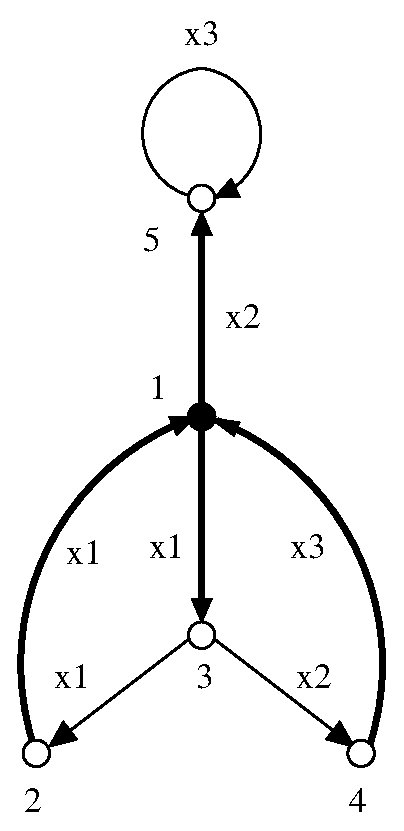
\includegraphics[scale=.52]{stallh1.eps}
\caption{Stallings automaton $\G_{A_1}$ for $H_1$}
\label{fig:stall1}
\end{subfigure}
\hspace{5mm}
\begin{subfigure}[b]{.25\columnwidth}
\psfrag{a}{$(1,2)$}
\psfrag{b}{$(2,3)$}
\psfrag{c}{$(3,1)$}
\psfrag{d}{$(4,5)$}
\psfrag{e}{$(1,5)$}
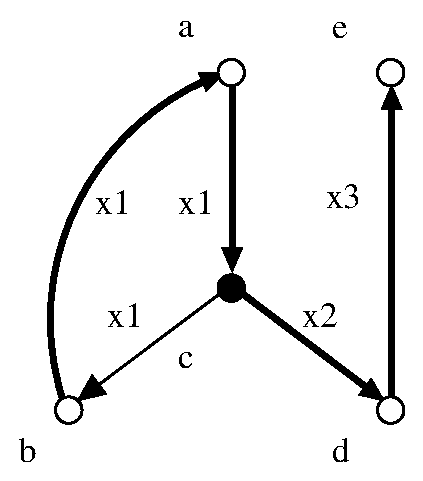
\includegraphics[scale=.52]{GxG-1.eps}
\caption{$\G_{A_1}\times \G_{A_1}$: connected component of $(3,1)$}
\label{fig:GxG-1}
\end{subfigure}
\hspace{5mm}
\begin{subfigure}[b]{.25\columnwidth}
\psfrag{a}{$(2,1)$}
\psfrag{b}{$(3,2)$}
\psfrag{c}{$(1,3)$}
\psfrag{d}{$(5,4)$}
\psfrag{e}{$(5,1)$}
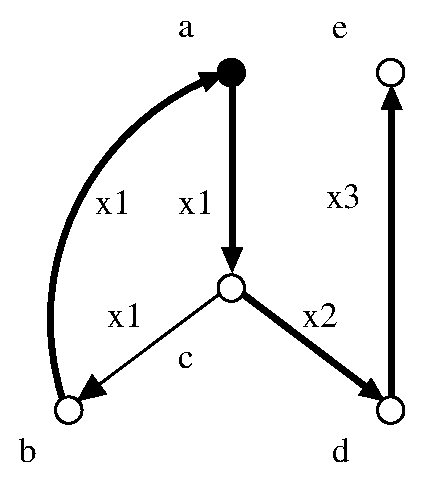
\includegraphics[scale=.52]{GxG-2.eps}
\caption{$\G_{A_1}\times \G_{A_1}$: connected component of $(2,1)$}
\label{fig:GxG-2}
\end{subfigure}
\end{center}
\caption{Example \ref{ex:f_1}.}\label{fig:stall}
\end{figure}

\begin{example}\label{ex:f_2}
Let $F_2$ be the free group on generators
$y_1,y_2,y_3,y_4$ with the subgroup $H_2 = \la h_1^{\prime},
h_2^{\prime},h_3^{\prime}\ra$, where
$h_1^{\prime}=y_2^2$,
$h_2^{\prime}=y_3y_4$ and
$h_3^{\prime}=y_1^2y_3y_1^{-1}y_2$.
The Stallings automata, $\G_{A_2}$ for $H_2$,
with maximal subtree $T_2$ highlighted and base vertex $1$, is shown
in Figure \ref{fig:stallh2}.
The set $L_{T_2}$ corresponding to the maximal subtree  $T_2$ is
 $L_{T_2}=
\{1, y_1, y_1^2,
y_2^{-1}, y_2^{-1}y_1, y_3 \}$.
Let the set of double coset representatives for $H_2$ be $S_2=S_2^{(1)}
\cup S_2^{(2)}$.

To find the normal form of $f_1^\prime=y_1^2y_3y_1^{-1}y_2y_3y_4y_1y_2
y_3y_4y_2^2$: use ${A_2}$ to read off the maximal acceptable
prefix $h= y_1^2y_3y_1^{-1}y_2y_3y_4=h_3^\prime h_2^\prime$ of $f_1^\prime$; and  the maximal
$L_{Q_2}$-prefix $p=y_1$ of the rest of $f_1^\prime$.  Next $q^{-1}=
y_2^{-2}y_4^{-1}y_3^{-1}y_2^{-1}$, so $g=y_2^{-2}y_4^{-1}y_3^{-1}
=h_1^{\prime -1}h_2^{\prime -1}$
and $t=y_2^{-1}$. This element will be represented by an element
of $S_2^{(2)}$, so we need to construct $\G_{A_2}\times \G_{A_2}$.
There are $7$  non-trivial, non-diagonal components. One is shown
in Figure \ref{fig:G2xG2-1} and the remaining
six in Figure \ref{fig:G2xG2-2}. In all cases the solid vertex
corresponds to the $\sim$ representative and connecting elements
are paths in the highlighted trees. Following Algorithm I, the
normal form of $f_1^\prime$ is
\[f_1^\prime=h yz^{-1} g^{-1},\]
where $y=y_1$, $z=y_2^{-1}$ and $yz^{-1}=y_1y_2\in S_2^{(2)}$: that is
\[f_1^\prime=h^\prime_3h_2^\prime y_1y_2 h_2^\prime h_1^\prime.\]
\end{example}
\begin{figure}
\begin{center}

\psfrag{y1}{$y_1$}

\psfrag{y2}{$y_2$}

\psfrag{y3}{$y_3$}

\psfrag{y4}{$y_4$}
\psfrag{1}{$1$}
\psfrag{2}{$2$}
\psfrag{3}{$3$}
\psfrag{4}{$4$}
\psfrag{5}{$5$}
\psfrag{6}{$6$}
\begin{subfigure}[b]{.3\columnwidth}
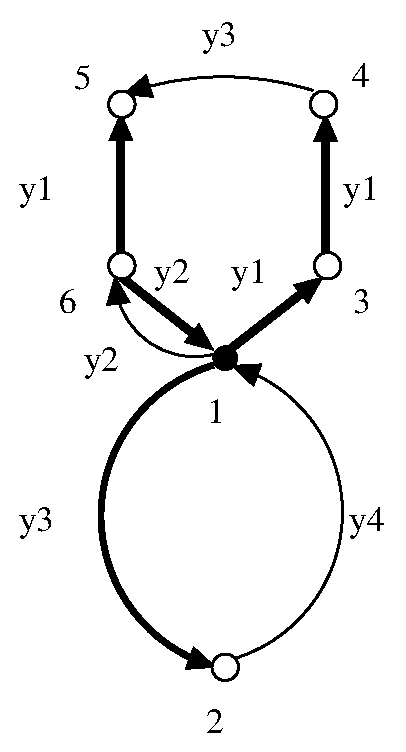
\includegraphics[scale=.52]{stallh2.eps}
\caption{Stallings automaton $A_2$ for $H_2$}
\label{fig:stallh2}
\end{subfigure}
\hspace{25mm}
\begin{subfigure}[b]{.3\columnwidth}
\psfrag{a}{$(5,3)$}
\psfrag{b}{$(6,1)$}
\psfrag{c}{$(1,6)$}
\psfrag{d}{$(3,5)$}
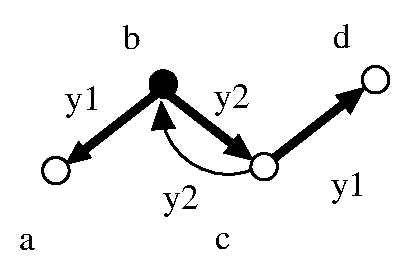
\includegraphics[scale=.52]{G2xG2-1.eps}
\caption{$\G_{A_2}\times \G_{A_2}$: connected component of $(6,1)$}
\label{fig:G2xG2-1}
\end{subfigure}
\end{center}
\caption{Stallings automata for Example \ref{ex:f_2}.}\label{fig:stallagain}
\end{figure}
\begin{figure}
\begin{center}

\psfrag{y1}{$y_1$}

\psfrag{y2}{$y_2$}

\psfrag{y3}{$y_3$}

\psfrag{y4}{$y_4$}
\psfrag{b}{$(1,3)$}
\psfrag{c}{$(3,4)$}
\begin{subfigure}[b]{.13\columnwidth}
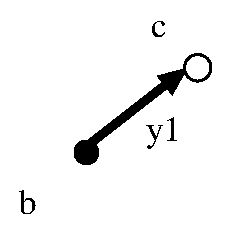
\includegraphics[scale=.5]{G2xG2-2.eps}
\caption{$(1,3)$}
\label{fig:G2xG2-2-1}
\end{subfigure}
\hspace{1mm}
\begin{subfigure}[b]{.13\columnwidth}
\psfrag{b}{$(3,1)$}
\psfrag{c}{$(4,3)$}
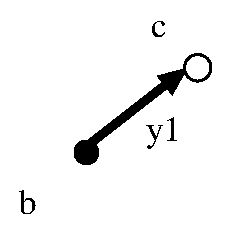
\includegraphics[scale=.5]{G2xG2-2.eps}
\caption{$(3,1)$}
\label{fig:G2xG2-2-2}
\end{subfigure}
\hspace{1mm}
\begin{subfigure}[b]{.13\columnwidth}
\psfrag{y1}{$y_3$}
\psfrag{b}{$(1,4)$}
\psfrag{c}{$(2,5)$}
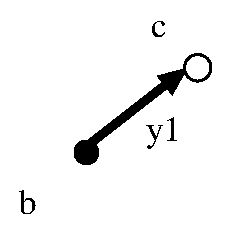
\includegraphics[scale=.5]{G2xG2-2.eps}
\caption{$(2,5)$}
\label{fig:G2xG2-2-3}
\end{subfigure}
\hspace{1mm}
\begin{subfigure}[b]{.13\columnwidth}
\psfrag{y1}{$y_3$}
\psfrag{b}{$(4,1)$}
\psfrag{c}{$(5,2)$}
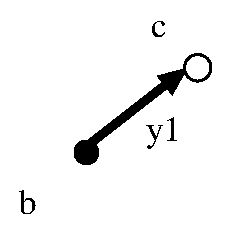
\includegraphics[scale=.5]{G2xG2-2.eps}
\caption{$(5,2)$}
\label{fig:G2xG2-2-4}
\end{subfigure}
\hspace{1mm}
\begin{subfigure}[b]{.13\columnwidth}
\psfrag{y1}{$y_1$}
\psfrag{b}{$(3,6)$}
\psfrag{c}{$(4,5)$}
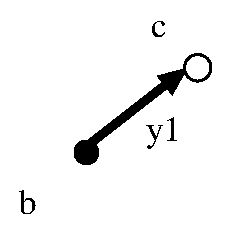
\includegraphics[scale=.5]{G2xG2-2.eps}
\caption{$(4,5)$}
\label{fig:G2xG2-2-5}
\end{subfigure}
\hspace{1mm}
\begin{subfigure}[b]{.13\columnwidth}
\psfrag{b}{$(6,3)$}
\psfrag{c}{$(5,4)$}
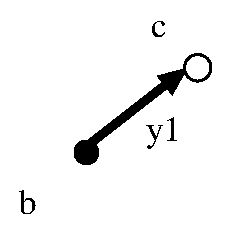
\includegraphics[scale=.5]{G2xG2-2.eps}
\caption{$(6,3)$}
\label{fig:G2xG2-2-6}
\end{subfigure}
\end{center}
\caption{Example \ref{ex:f_2}: connected components of $\G_{A_2}\times \G_{A_2}$.}\label{fig:G2xG2-2}
\end{figure}

In fact if we don't require uniqueness of representatives then
there is a much simpler algorithm to write words in normal form.
This simply finds the maximal prefix $h_1$ of $w$  accepted  by
$A$  and so $w=h_1\circ v$. It then finds the maximal prefix $p$
of $v^{-1}$ accepted by $A$. Setting $h_2=p^{-1}$ gives
$w=h_1\circ d \circ h_2$, for some uniquely determined word $d$,
which is a (non-unique) double coset representative.

%%%%%%%%%%%%%%%%%%%%%%%%%%%%%%%%%%%%%%%%%%%%%%%%%
\section{The generalised folding process}\label{sec:foldings}

Recall from above that $F_1$ and $F_2$ are free groups on finite sets
$X_1$ and $X_2$, respectively;
 $H_1 \leq F_1$ and $H_2 \leq F_2$ are subgroups of rank $m$, freely
generated by $\{h_1,\ldots, h_m\}$ and $\{h_1^\prime,\ldots ,h_m^\prime\}$.
The isomorphism from $H_1$ to $H_2$ which maps $h_i$ to $h_i^\prime$ is
denoted $\phi$.

Now let
$Z=\{z_1,\ldots, z_m\}$ be a set disjoint from $X_1\cup X_2$. Then there
is an isomorphism $\phi_1:\FF(Z)\maps H_1$, such that $\phi_1(z_i)=h_i$,
 and an isomorphism $\phi_2:\FF(Z)\maps H_2$, such that $\phi_2(z_i)
=h_i^\prime$, $i=1,\ldots, m$.
 Let $G$ be the free product with amalgamation:
${G = F_1 \underset{H_1=H_2}{\ast} F_2}$.  Then $G$ has a
 presentation
\[\la X_1\cup X_2\cup Z  | h_i =z_i= h_i', i=1 \ldots m\ra.\]

\begin{definition}\label{def:dcnf}
 Let $D_1$ and $D_2$ be sets of  double coset representatives for
$H_1\le F_1$ and $H_2\le F_2$, respectively.
A word $w\in \FF(X_1\cup X_2\cup Z)$ is in
\emph{double coset normal form}, or \emph{dc-normal form}, with
respect to $D_1\cup D_2$, if
$w = h_{0}p_1h_{1}p_2 \cdots h_{k-1}p_kh_{{k}}$, $k\ge 0$,   where 
\be[(a)]
\item $h_i$ is a reduced word in $\FF(Z)$, for $i=0,\ldots, k$;
\item  $p_i  \in D_1\cup D_2$ and $p_i\neq 1$, for $i=1,\ldots, k$,  and
\item if  $p_i\in D_j$ then $p_{i+1}\notin D_j$, for $j\in \{1,2\}$
and $i=1,\ldots ,k-1$.
\ee
\end{definition}
From now on when we say ``normal form'' we mean ``double coset normal form'' unless
we explicitly say something to the contrary.
\begin{theorem}\label{thm:dcnf} Let $D_1$ and $D_2$ be sets of  double coset representatives for
$H_1\le F_1$ and $H_2\le F_2$, respectively. 
Then every element of $G$ is represented by a unique element of
$\FF(X_1\cup X_2\cup Z)$ in double coset normal form, with respect
to $D_1\cup D_2$.
\end{theorem}
\begin{proof}
To see that every $g\in G$ can be written in dc-normal form, first
write $g$ in reduced form. If the reduced form of $g$ is the empty
word then this is also the dc-normal form; with $k=0$ and $h_0=1$. 
Otherwise we have $g=f_1\cdots f_t$, where $f_i$ is in $F_{j_i}$, for
$j_i\in \{1,2\}$. In this case, let $a_is_ib_i$
be the double coset representative of $f_i$, where 
$a_i,b_i\in H_{j_i}$ and $s_i\in D_{j_i}$. For $i=1,\ldots ,t$,
 let $z^{\prime}_i=\phi_j^{-1}(a_i)$ and
$z^{\prime\prime}_i=\phi_j^{-1}(b_i)$. For $i=1,\ldots ,t-1$, let 
$z_i$ be the free reduction of $z^{\prime}_iz^{\prime\prime}_{i+1}$, 
and let $z_0=z^{\prime}_1$ and $z_t=
z^{\prime\prime}_t$. 
 If $t=1$ and $f_1\in H_{j_1}$ then $a_1=f_1$, $s_1=1$, $b_1=1$ and 
the dc-normal form of $g$ is $z_0$. Otherwise, for all $i\ge 1$, we 
have $f_i\notin H_1\cup H_2$, so $s_i\neq 1$ and 
\[z_0s_1z_1\cdots z_{t-1}s_tz_t\]
is a dc-normal form for $g$.

Now suppose that $w$ and $w^\prime$ are words in dc-normal form and that
$w=_G w^\prime$. We show by induction on $k$ that $w=w'$. 
Let $w=h_{0}p_1h_{1}p_2 \cdots h_{k-1}p_kh_{{k}}$,
and $w^\prime =h_{0}^\prime p_1^\prime h_{1}^\prime  p_2^\prime
\cdots h_{k-1}^\prime p_k^\prime h_{{k^\prime}}^\prime$, where
$h_i, h_i^\prime\in \FF(Z)$ and $p_i,p_i^\prime\in S_1\cup S_2$.
%If $w$ is the empty word then $k=0$ and $h_0=1$ and in this case it follows
%from \cite[Chapter IV, Theorem 2.6]{LS} that $k'=0$ and $h'_0=1$, so 
%$w=w'$. Hence we  assume that either $k>0$ or $h_0\neq 1$. 
If $k=0$ let $f_1=\phi_1(h_0)$ and, if $k>0$, 
let $f_1=\phi_{j_1}(h_0)p_1\phi_{j_1}(h_1)$, where $p_1\in F_{j_1}$. 
 In addition, if $k>0$,  
 for fixed $i\ge 2$, assuming that $p_i\in F_{j_i}$, 
let $f_i=p_i\phi_{j_i}(h_i)$.
 Then $f_1\cdots f_k$, is
a reduced form for the element $w\in G$. Similarly, we obtain a reduced
form $f_1^\prime \cdots f_{k^\prime}^\prime$ for $w^\prime=_G w$. 

If $k=0$ then we have $w=_G f_1=\phi_1(h_0)\in H_{1}$, and since all 
reduced forms representing an element have the same length, $k'=0$ or $1$. 
Moreover, as $f'_1=_G w\in H_1$ we have 
 $k^\prime =0$ and $w^\prime=_G f_1^\prime=\phi_1(h_0^\prime)\in H_1$.
As $H_1$ embeds in $G$ this implies that $\phi_1(h_0)=\phi_1(h'_0)$, so
$w=h_0=h'_0=w'$. Thus the result
holds when $k=0$ and we may assume inductively that $k>0$ and the result holds
for elements represented by normal forms of length less than $k$.

Comparing the lengths of reduced forms, we have $k=k^\prime$.
Moreover, $1=_G w^\prime w^{-1}= f_1^\prime \cdots f_{k}^\prime
f_k^{-1}\cdots f_1^{-1}$, so by \cite[Chapter IV, Theorem 2.6]{LS}, 
we have $ f_{k}^\prime f_k^{-1}\in H_{j_k}$, where $j_k=1$, or $2$. Hence, for
some $a, b\in H_{j_k}$ we have $p_k^\prime=a p_k b$. Therefore $p_k^\prime =p_k$,
and now, as $p_k$ is a double coset representative and  $ f_{k}^\prime f_k^{-1}\in H_{j_k}$,
it follows that $h_k=h_k^\prime$. Hence $f_1\cdots f_{k-1}=
f_1^\prime \cdots f_{k-1}^\prime$ and, applying the inductive hypothesis,
  we see that $w=w^\prime$, as required.
\end{proof}


\begin{example}\label{ex:g}
Let $F_i$ and $H_i$ be given in Examples \ref{ex:f_1} and
Example \ref{ex:f_2}, and
let $f_1$ and $f_2$ be the elements of $F_1$ in Example \ref{ex:f_1} and
$f_1^\prime\in F_2$ as in Example \ref{ex:f_2}.
Set $z_i = h_i = h_i^{\prime}$ for $i= 1,2,3$.

Let $g =f_1 f_1^\prime f_2$; then we have
\begin{align*}
f_1&=(h_2^{2}h_1) x_1x_3x_1 (h_1^{-1}h_3^{-1})\\
&=z_2^2z_1  x_1x_3x_1z_1^{-1}z_3^{-1},\\
f_2&=(h_3^{-1}h_2^{-1}) x_1^{-1}\\
&=z_3^{-1}z_2 x_1^{-1}\textrm{ and }\\
f_1^\prime&=h^\prime_3h_2^\prime y_1y_2^{-1} (h_1^\prime)^{-1}(h_2^\prime)^{-1}\\
&= z_3z_2 y_1y_2^{-1} z_1^{-1}z_2^{-1}.
\end{align*}
Therefore the double coset normal form of $g$ is
\[g=z_2^2 z_1  x_1 x_3 x_1 z_1^{-1}
z_2y_1y_2^{-1} z_1^{-1}z_2^{-1}
z_3^{-1}z_2^{-1} x_1^{-1}.
\]
\end{example}


The object of this section is to construct an automaton which will accept a word
$w$ in double coset normal form if and only if it belongs to a
given subgroup $K$ of $G$. The idea is to do this by starting with the
flower automaton for the generators of $K$, written in (double
coset) normal form; carrying out Stallings folding as usual to
produce an inverse automaton; and next
adding some additional paths to allow normal forms to be read.
This may introduce new non-determinism in some  states (i.e. edges
which may be folded), so the resulting automaton must be folded
again. The result of the final folding is the candidate automaton.

 Suppose $L$ is the
language accepted by the flower automaton of $K$. The image of $L$ under
the canonical map to $G$ is $K$. All the stages of our generalised folding
process will preserve this image, so our final automaton will accept a language
$L_1$ which also maps to $K$. We must then prove that, if $w$ is a word
in normal form which represents an element of $K$ then $w$ is in $L_1$. It will
therefore suffice to show that, if $u$ is any word in $L_1$ then the
normal form of $u$ is also in $L_1$.

\begin{comment}
Let $S_1=S(H_1)$ and $S_2=S(H_2)$ be sets of elements of $F_1$ and 
$F_2$ corresponding to $H_1$ and $H_2$, as in Definition \ref{def:dcreps}. 
%Then $D_1=S_1\cup \{1\}$ and $D_2=S_2\cup \{1\}$ are sets of 
%double coset representatives for 
%$H_1\le F_1$ and $H_2\le F_2$, respectively. 
Denote $S= S_1 \cup S_2\cup \{1\}$. Let $A_k$ be the
Stallings automaton for $H_k$ and let $T_k$ be a spanning tree for
the associated graph $\G_{A_k}$, $k=1,2$. The alphabet of $A_k$ is
$X_k$ and the set of states of $A_k$ is denoted $Q_k$.

%\subsection{Construction of the double coset normal form}\label{sub:construction_dcnf}}
Suppose that $g \in G$ and $g=g_1\cdots g_t$ is the reduced form of $g$. 
As in the proof of Theorem \ref{thm:dcnf} we may use the reduced form
to construct the double coset normal form of $g$. 
Write each syllable $g_i$ of $g=g_1\cdots g_t$ in normal form
using the algorithm I above. This gives
$g_i=h_{i,1}d_ih_{i,2}$, with $d_i\in S$ and $h_{i,j}\in H_1\cup
H_2$. Using $\phi_1^{-1}$ or $\phi_2^{-1}$, as appropriate, we now
write $h_{i,1}$ and $h_{i,2}$ as reduced words in $\FF(Z)$. For
$i=1,\ldots , t-1$, we reduce the word $h_{i,2}h_{(i+1),1}\in
\FF(Z)$ to give a reduced word $h_i\in \FF(Z)$ and set $h_0=h_{1,1}$
and  $h_{t+1}=h_{t,2}$. Then $g$ has normal form $h_0d_1h_1\cdots
d_th_{t+1}$.
\end{comment}


\subsection{Double coset automata}\label{sec:dca}
%
%
Let $K=\la k_1, \ldots , k_s\ra$, where $k_i$ is an element of $G$
written in normal form: say
\begin{equation}\label{eq:k-form}
k_i= h_{i,0}t_{i,1}h_{i,1}\cdots t_{i,m_i}h_{i,m_i},
\end{equation}
with $m_i\ge 0$, $h_{i,j}\in \FF(Z)$, $t_{i,j}\in S_1\cup S_2$, such that
if $m_i=0$ then
$h_{i,0}\neq 1$ (since we may discard any generators of $K$ which equal
the empty word). Denote
by $\hat K$ the subgroup of  $\FF(X_1\cup X_2 \cup Z)$ generated by
$k_1, \ldots , k_s$. Let $\S=(X_1\cup X_2 \cup Z)^{\pm 1}$.
Let $\cF(K)$ be the flower automaton of $\hat K$, and let
$\G$ be the corresponding rooted graph. If $e$ is an edge of $\G$ then
$e$ is labelled by a letter of $\S$
occuring in $h_{i,j}$ or $t_{i,j}$, for some $i,j$, as in
\eqref{eq:k-form}. If $e$ is labelled by a letter of $Z$ we say $e$ has {\em type} $Z$.
 %and define $c(e)=(0,0)$.
If $e$ is labelled by a letter of $X_k$ occuring in $t_{i,j}$, we
say $e$ has {\em type} $X_k$, $k = 1,2$.

Now let $\G_K$ be the Stallings folding of the graph $\G$.  Then
 $\G_K$ is inverse and $\pi(L(\G_K))=K$. However
$L(\G_K)$ does not, in general, contain all normal forms of elements of $K$.
We wish to transform $\G_K$ to allow it to accept normal forms of
elements of $K$. In outline this transformation process consists of
running the loop below, on input $\G_K$,
until it halts, at which point we shall show that we have an
inverse automaton which accepts  normal forms of elements of $K$.
Begin by setting $\G_K=\D_{(0)}$; so  that $\D_{(0)}$ is an inverse automaton, with alphabet $\S$
and $\pi(L(\D_{(0)}))=K$. \\[1em]
\textbf{Generalised Folding Loop.}
Set $n=0$.
\be[Step 1]
\item\label{it:gf1} Apply Algorithm II below to add new paths to $\D_{(n)}$ which allow normal forms of labels
of certain paths to be read. %If at least one path has been added,
Call the result $\D_{(n)}^{\prime\prime}$.
%If no paths are added at this step,
%halt and output  $\G_K^{(n)}$.
\item\label{it:gf2} Construct the Stallings automaton $\D_{(n+1)}$
of $\D_{(n)}^{\prime\prime}$. If $\D_{(n+1)}$ and
$\D_{(n)}$ have the same
 number of
$X_1$ and $X_2$ components (see below) then output $\D_{(n+1)}$
and stop. Otherwise, add $1$ to $n$ and  return to   \ref{it:gf1}.
\ee

Algorithm II below describes exactly how to carry out Step 1 of
this loop. Since Step 1 may run more than once,  the input to 
Algorithm II is assumed to be an arbitrary inverse automaton $\D$,
with alphabet $\S$ and $\pi(L(\D))=K$. The output of Algorithm II
is a rooted,
labelled, involutive automaton $\D''$, with the same alphabet, which may
fail to be deterministic. This automaton $\D''$ is input to \ref{it:gf2}, 
where it is folded. We shall show that, if we start as above
with $\G_K=\D_{(0)}$,  the Generalised Folding Loop halts, at some $n<\infty$; at
which point $\D_{(n+1)}$ is an inverse automaton which accepts the
normal form of every element of $K$. \\[1em]

\noindent\textbf{Algorithm II}. \\

Here each step of the algorithm is justified as it is introduced. A 
summary of the algorithm is given in Section \ref{sub:summaryII}.  
Let $\D$ be an inverse automaton, with alphabet $\S$ and
start and final state $1$, such that
$\pi(L(\D))=K$.
For $k=1,2$, let $\D_k$ be the graph formed from $\D$ by removing all edges of
type $X_{k^\prime}$, where $k\neq k^\prime$. An $X_k$ component of
$\D_k$ is the subgraph of $\D$ formed from a connected component
of $\D_k$ by removing all leaves which are incident to edges of
type $Z$, and then repeating the process till there are no such
leaves left. Given an $X_k$ component $\T$ of $\D_k$,  a
{\em boundary vertex} of $\T$ is defined to be a vertex
$\a$ such that $\a$ is incident, in $\D$, to a vertex which does not
belong to $\T$.
 We shall modify each  $X_k$ component $\T$ of $\D_k$ so that if $p$ is a path,
from a  boundary vertex $u$  to a boundary vertex $v$ of $\T$,
then the normal form  of  the label $l(p)$ of $p$ is the label of
a path from $u$ to $v$. Throughout the modification process we
keep track of the boundary vertices, so that once modification is
complete the $X_k$ components can be reassembled, by attaching as
they did in $\D$. The modification of an $X_k$ component $\Theta$
of $\D_k$ consists of
five steps, producing new graphs $\T_1$, $\T_2$, $\T_3$, $\T_4$
and $\T_5$. In each case there is a canonical morphism $\theta_i$
from $\T_{i-1}$ to $\T_i$ and,
 (writing $\T=\T_0$)
we define the {\em boundary vertices} of $\T_{i}$ to be the vertices $\theta_{i}(v)$
of $\T_i$, such that $v$ is a boundary vertex of $\T_{i-1}$. Moreover the
 images $\theta_i\circ \cdots\circ \theta_1(v)$ of vertices of $\T$ in $\T_i$
will be referred to as  {\em vertices of} $\T$.


The modification process is followed by a ``reassembly'' phase, in which
we reconnect the $X_k$ components of $\D$, 
to form the output of the algorithm. 
To enable the reassembly the algorithm records, when constructing 
$\Theta_{i}$ from $\Theta_{i-1}$, the inverse images of vertices of 
$\Theta_{i}$ under the map $\theta_i$. We leave details of the
construction of these inverse image sets to the the summary
in 
Section \ref{sub:summaryII}. 
 
Let $\T$ be an $X_k$ component of $\D_k$.
\\[1em]

\noindent\textbf{Modification 1: $\T\leadsto \T_1$.}\\
This step involves the addition of paths labeled by $X_k$-words corresponding to
$z$-edges of an $X_k$ component.

 If $(\a,z,\b)$ is an
edge of $\T$ labelled by an element $z\in Z$ then add a path from
$\a$ to $\b$ labelled by $\phi_k(z)$ to the graph $\T$. Do this
for all such edges and call the result
$\T_1^\prime$. Fold $\T_1^\prime$ to form the graph
$\T_1$. (See Figure \ref{fig:alg2-1}.)
\begin{figure}
\begin{center}
\psfrag{a}{$\a$}
\psfrag{b}{$\b$}
\psfrag{h}{$z$}
\psfrag{w}{$w$}
\begin{subfigure}[b]{.25\columnwidth}
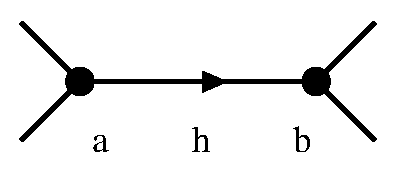
\includegraphics[scale=.5]{alg2-1a.eps}
\label{fig:alg2-1a}
%\caption{}
\end{subfigure}
\raisebox{3ex}{$\leadsto$}
\begin{subfigure}[b]{.25\columnwidth}
\psfrag{a}{$\a$}
\psfrag{b}{$\b$}
\psfrag{h}{$z$}
\psfrag{w}{$w$}
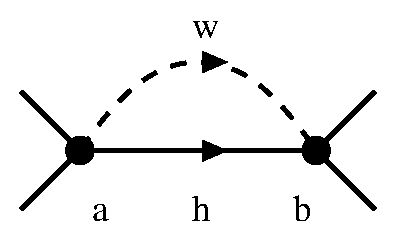
\includegraphics[scale=.5]{alg2-1b.eps}
\label{fig:alg2-1b}
%\caption{}
\end{subfigure}
\end{center}
\caption{$\Theta$ to $\Theta_1$: $w=\phi_k(z)$.}\label{fig:alg2-1}
\end{figure}
Let $\theta_1$ be the compostion of the inclusion map from 
$\Theta$ to $\Theta'_1$ with the folding morphism from $\Theta'_1$ to
$\Theta_1$. If $\a$ and $\b$ are vertices of $\Theta$ then,
since $\theta_1$ is a morphism
$\pi(L(\Theta, \a,\b))\subseteq \pi(L(\Theta_1,\theta_1(\a),\theta_1(\b)))$.
On the other hand if $w$ is in  $L(\Theta_1,\theta_1(\a),\theta_1(\b))$
then, since $\Theta_1$ is a folding of $\Theta_1^\prime$,
 there is a path labelled $w^\prime$ from $\a$ to $\b$ in $\Theta_1^\prime$,
such that $\pi(w^\prime)=\pi(w)$.
By construction then there exists  a path $w^{\prime\prime}$ from
$\a$ to $\b$ in $\Theta$, such that $\pi(w^{\prime\prime}) =
\pi(w^\prime)$. Hence $\pi(L(\Theta_1,\theta_1(\a),\theta_1(\b)))
= \pi(L(\Theta, \a,\b))$.  \\[1em]
%%%

\noindent\textbf{Modification 2: $\T_1\leadsto \T_2$.}\\
Here we add to $\T_1$ paths labelled by $\phi_k^{-1}$ images of labels of simple
paths in $\T_1\times \G_{A_k}$, from $(\a_i,1)$ to $(\a_j,1)$; for
appropriate $i,j$.
 Let $\cP_1=\T_1\times \G_{A_k}$. Then there is a path
 labelled $w$ from $\a$ to $\b$
in $\T_1$ and a path labelled $w$ from $\a^\prime $
to $\b^\prime$ in $\G_{A_k}$ if and only if there is a path
labelled $w$ from $(\a,\a^\prime)$ to $(\b,\b^\prime)$ in $\cP_1$.
 We shall
use this property of $\cP_1$ to determine which new paths to add  to
$\T_1$. Choose a spanning  forest $\U_1$ of  $\cP_1$. Next
 order the vertices of
$\T_1$: say these are $\a_0,\ldots, \a_t$, in the order written.

Let $\a_i$, $\a_j$ be vertices of  $\T$  with $i\le j$. If
\begin{itemize}
\item
 there
exists a simple path $p$ in $\cP_1$ from $(\a_i,1)$ to $(\a_j,1)$ and
\item
$p$ does not contain a vertex $(\a_k,1)$ with $k\in\{i,j\}$
\end{itemize}
then let $l_p\in \FF(X_k)$ be the label of $p$ and let
$w_p=\phi_k^{-1}(l_p)\in \FF(Z)$. Let $q$ be a path (disjoint from
$\T_1$) of length $|w_p|$ and with label $w_p$. Identify the
initial vertex of $q$ with $\a_i$ and the terminal vertex of $q$
with $\a_j$. (See Figure \ref{fig:alg2-2}.)
\begin{figure}
\begin{center}
\psfrag{a}{$\a$}
\psfrag{b}{$\b$}
\psfrag{h}{$l_p$}
\psfrag{w}{$w_p$}
\psfrag{ai}{$(\a_i,1)$}
\psfrag{bi}{$(\a_j,1)$}
\psfrag{1}{$1$}
\psfrag{Th1 to Th2}{$\T_1\leadsto \T_2$}
\psfrag{cP}{$\cP_1$}
\psfrag{G_A}{$\G_{A_k}$}
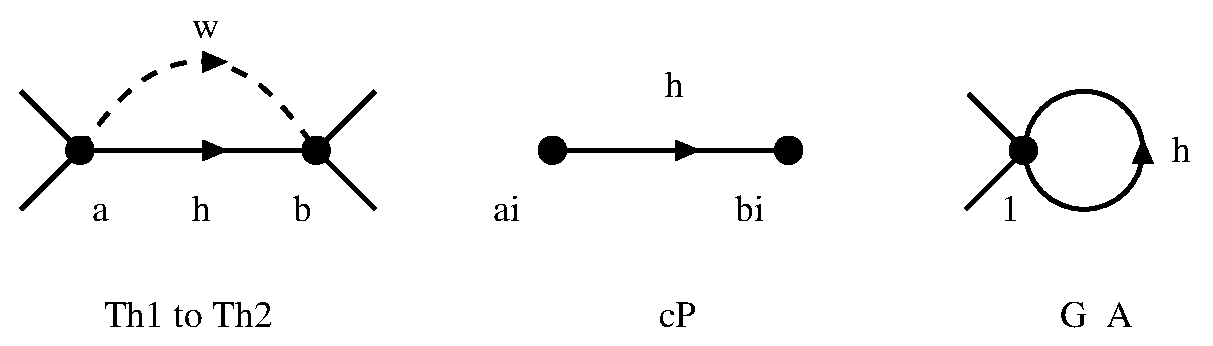
\includegraphics[scale=.5]{alg2-2.eps}
\end{center}
\caption{$\Theta_1$ to $\Theta_2$: $w_p=\phi_k^{-1}(l_p)$.}\label{fig:alg2-2}
\end{figure}
Repeat this process for all simple paths from  $(\a_i,1)$ to
$(\a_j,1)$, over all pairs of vertices $\a_i$, $\a_j$ of $\T$,
with $i\le j$. There are finitely many simple paths in $\cP_1$ so
this process terminates. Call the result $\T_2^\prime$. Then
$\T_1$ is a subgraph of $\T_2^\prime$. Now fold $\T_2^\prime$ to
give a new graph $\T_2$. The composition $\theta_2$ of the the
embedding map of $\T_1$ into $\T_2^\prime$ with the canonical
morphism from $\T_2^\prime$ to $\T_2$ is a morphism from $\T_1$ to
$\T_2$.
 Moreover, if $\a$ and
 $\b$ are
%boundary
 vertices of $\T_1$ and
a path $q$ from $\a$ to $\b$, with label $w_p$, is added to $\Theta_1$
in forming $\Theta_2$, then there is a path $p$ in $\Theta_1$ with
$\pi(l(p))=\pi(w_p)$. Thus the argument of the previous case shows that
$\pi(L(\T_1,\a,\b))=\pi(L(\T_2,\theta_2(\a),\theta_2(\b)))$.\\[1em]

\noindent\textbf{Modification 3: $\T_2\leadsto \T_3$.}\\
At this stage we add $\phi_k^{-1}$ images of paths in $\T_2\times
\G_{A_k}$ related to edges of this graph which do not belong to
its spanning subforest and which belong to paths which project 
to closed paths 
based at $1$, in $\G_{A_k}$.

As the edges added to $\T_1$ to form $\T_2$ are all labelled by elements
of $Z$, and all edges of $\G_{A_k}$ are labelled by elements of $X_k$
the graphs $\cP_1=\T_1\times \G_{A_k}$ and $\cP_2=\T_2\times \G_{A_k}$ differ only
in that the second may have some new isolated vertices. Therefore we may
choose a spanning forest $\U_2$ of $\cP_2$ consisting of the spanning
forest $\U_1$ of $\cP_1$ with some new isolated vertices if necessary.
If $\cP_2$ is a forest then
$\cP_2=\U_2$, there is nothing to do at the
this stage, and we immediately set $\T_3=\T_2$. Otherwise, suppose
that $e$ is an edge of $\cP_2$ which does not belong to $\U_2$ but
which does belong to a component $\Xi$  of $\cP_2$ containing a
vertex $(\a,1)$, for some vertex $\a$ of $\T$. Let $(\a,1)$ be
such a vertex and let $e=((\a_i,\b_1), x, (\a_j,\b_2))$ be an edge
in the same component of $\cP_2$ as $(\a,1)$,
 with label $x$ in $X_k$.
%Let
%$\a_m$ be the minimal vertex of $\T_2$ (necessarily also a vertex
%of $\T_1$)  such that $(\a_m,1)$ belongs to $\Xi$.
 Let $p_i$ be
the path in $\U_2$ from $(\a,1)$ to $(\a_i,\b_1)$ and let $p_j$ be
the path in $\U_2 $ from  $(\a_j,\b_2)$ to $(\a,1)$ and let $l_i$
and $l_j$ be the labels of $p_i$ and $p_j$, respectively. Then
$p_i,e,p_j$ projects to a closed path in $\G_{A_k}$, based at $1$,
with label $h_e=l_i x l_j \in H_k\subseteq F_k$. Moreover
$p_i,e,p_j$ projects to a closed path in $\T_2$, based at $\a$,
also with label $h_e$. Let $w_e=\phi_k^{-1}(h_e) \in \FF(Z)$ and let
$q$ be a path (disjoint from $\T_2$) of length $|w_e|$ and with
label $w_e$. Identify the initial and terminal vertices of $q$ to
the vertex  $\a$ of $\Theta_2$. (See Figure \ref{fig:alg2-3}.)
\begin{figure}
\begin{center}
\psfrag{a}{$\a$}
\psfrag{b}{$\b$}
\psfrag{x}{$x$}
\psfrag{h}{$h_e$}
\psfrag{w}{$w_e$}
\psfrag{li}{$l_i$}
\psfrag{lj}{$l_j$}
\psfrag{ai}{$(\a_i,\b_1)$}
\psfrag{bi}{$(\a_j,\b_2)$}
\psfrag{(a,1)}{$(\a,1)$}
\psfrag{1}{$1$}
\psfrag{Th2 to Th3}{$\T_2\leadsto \T_3$}
\psfrag{cP}{$\cP_2$}
\psfrag{G_A}{$\G_{A_k}$}
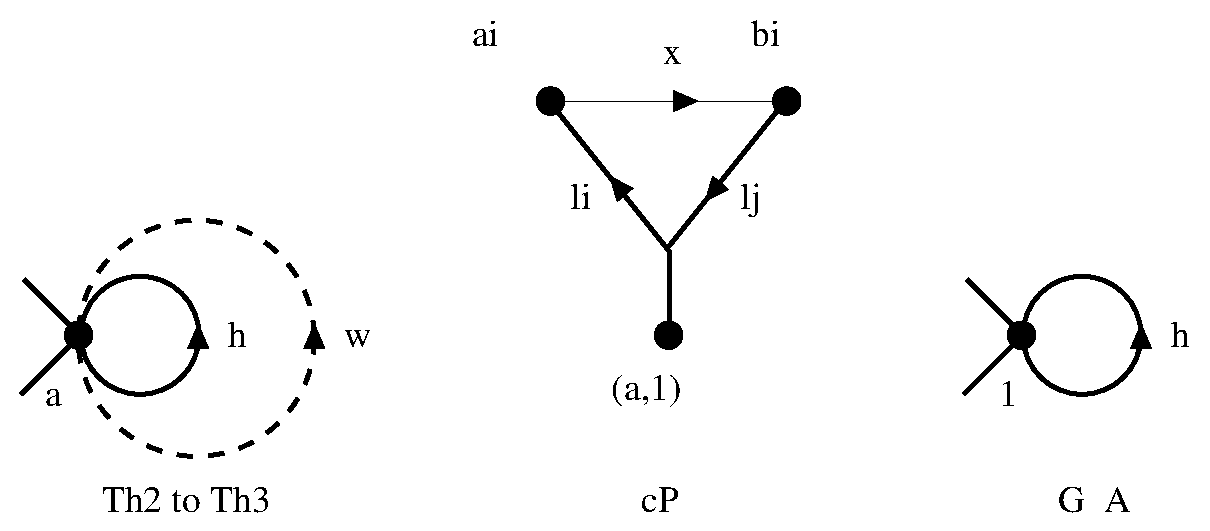
\includegraphics[scale=.5]{alg2-3.eps}
\end{center}
\caption{$\Theta_2$ to $\Theta_3$: $h_e=l_ixl_j$,
$w_e=\phi_k^{-1}(h_e)$.}\label{fig:alg2-3}
\end{figure}
Repeat this process for all such edges $e$ and vertices $(\a,1)$
of $\cP_2$,  fold the resulting graph, and denote the result by
$\T_3$. (In practice it's not necessary to repeat this process for
{\em all} such vertices $(\a,1)$ in $\Xi$: but it makes some
arguments  later easier if we assume that we do so.) As in the
previous case there is a natural morphism $\theta_3$ from $\T_2$
to $\T_3$. Again, if $q$ is a path added to $\Theta_2$ in forming
$\T_3$ then there is a path $p$ in $\T_2$, with the same end points
as $q$, such that $\pi(l(p))=\pi(l(q))$. Hence, as before, for all
vertices   $\a$, $\b$ of $\T_2$,
$\pi(L(\T_2,\a,\b))=\pi(L(\T_3, \theta_3(\a),\theta_3(\b)))$.\\[1em]

\noindent\textbf{Modification 4: $\T_3\leadsto \T_4$.}\\
Next we wish to add paths to $\T_3$ that allow us to read the normal
forms of words $w$ which are readable by $\T_3$ and readable,
but not accepted, by $\G_{A_k}$.
 Let
$\cP_3=\T_3\times \G_{A_k}$.
As before we may choose a spanning forest $\U_3$ of $\cP_3$ which
consists of $\U_2$ and some additional isolated vertices.

Recall that we have fixed a spanning subtree
$T_k$ of $\G_{A_k}$.
Let $\d=(\a_j,\b)$ be a vertex of $\cP_3$, with $\b\neq 1$, which lies
in a connected component of $\cP_3$ containing a vertex  $\g=(\a_i,1)$,
for some vertices $\a_i$ and $\a_j$ of $\T$.
Let $b$ be the label of the path in $T_k$ from $1$ to $\b$.
 If $\cP_3$ contains a simple
path from $(\a_i,1)$ to $(\a_j,\b)$, with label $b$,  then
 say that $\cP_3$ {\em covers} the pair $\g,\d$.
If all such pairs of vertices are covered by $\cP_3$ then set $\T_4=\T_3$.
Otherwise
let $p$ be the simple path in $\U_3$ from a
vertex $\g=(\a_i,1)$ to a vertex $\d=(\a_j,\b)$, where $\g,\d$
is not covered by $\cP_3$.
 Let
$p$ have label $a$.
Then $ab^{-1}=h\in H_k$. Let
$w=\phi_{k}^{-1}(ab^{-1})
\in \FF(Z)$ and let $q$ be a path (disjoint from $\T_3$)
with label $wb$. Identify the initial
and terminal vertices of $q$ with vertices $\a_i$ and $\a_j$ of $\T_3$,
respectively, to form a new graph $\T_3^\prime$.
(See Figure \ref{fig:alg2-4}.)
\begin{figure}
\begin{center}
\psfrag{ai}{$\a_i$}
\psfrag{bi}{$\a_j$}
\psfrag{g}{$a$}
\psfrag{h}{$b$}
\psfrag{w}{$wb$}
\psfrag{(ai,1)}{$(\a_i,1)$}
\psfrag{(aj,b)}{$(\a_j,\b)$}
\psfrag{1}{$1$}
\psfrag{b}{$\b$}
\psfrag{Th3 to Th4}{$\T_3\leadsto \T_4$}
\psfrag{U3 in cP}{$\U_3\subseteq \cP_3$}
\psfrag{Tk in G_A}{$T_k\subseteq \G_{A_k}$}
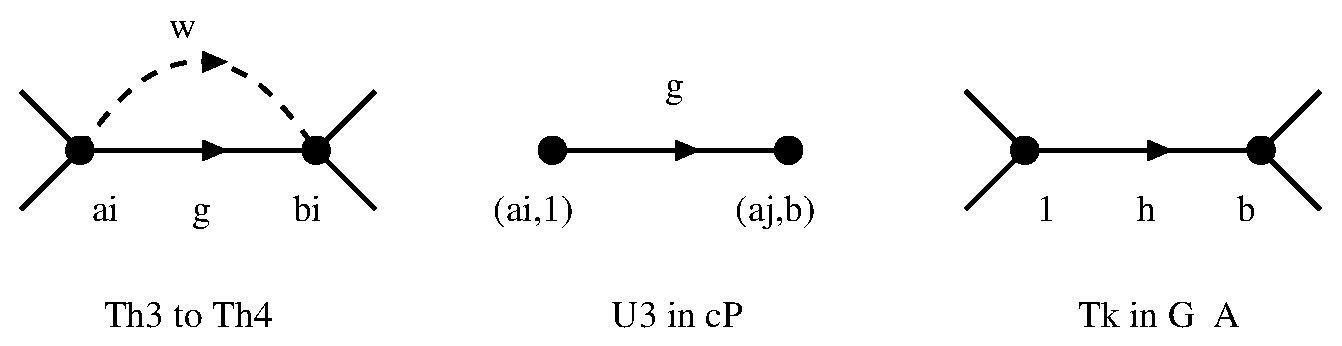
\includegraphics[scale=.5]{alg2-4.eps}
\end{center}
\caption{$\Theta_3$ to $\Theta_4$: $w=\phi_k^{-1}(ab^{-1})$.}\label{fig:alg2-4}
\end{figure}

As $\pi(a)=\pi(wb)\in G$, if $L_3$ and $L_3^\prime$ are the languages
accepted by $(\T_3,\a,\b)$ and $(\T_3^\prime,\a,\b)$, for some
vertices $\a,\b$ of $\T_3$, then $\pi(L_3)=\pi(L_3^\prime)$.
Repeat this process for all pairs of  vertices which are not
covered by $\cP_3$  and fold
the result to form the graph $\T_4$. Again there is a natural
morphism $\theta_4$ from $\T_3$ to $\T_4$. If $L_4$ is the
language accepted by $(\T_4,\theta_4(\a),(\b))$, for some
vertices $\a,\b$ of $\Theta_3$, then
we have $\pi(L_3)=\pi(L_4)$, as in previous cases.\\[1em]


\noindent\textbf{Modification 5: $\T_4\leadsto \T_5$.}\\
Finally we wish to add paths which allow double coset representatives
of type $2$ to be read.
Let $\cP_4=\T_4\times \G_{A_k}$ and choose a spanning forest $\U_4$ for
$\cP_4$.

Let $(\e_1,\e_2)\in P\subseteq V(\G_{A_k}\times \G_{A_k})$, let 
 the $\sim$ representative of $(\e_1,\e_2)$ be $(\xi_1,\xi_2)$ and  
set $a_1=w(\xi_1)$ and $a_2=w(\xi_2)$.
By definition of $\sim$ there are  paths in $\G_{A_k}$,
with label
$c=c(\e_1,\e_2)$, from $\e_1$ to $\xi_1$ and $\e_2$ to $\xi_2$.

Assume that, for  some vertices $\a_1,\a_2, \b$ of $\T$, there exist vertices
$(\a_1,1)$, $(\a_2,1)$, $(\b,\e_1)$ and $(\b,\e_2)$, and simple 
paths   $p_1$, from $(\a_1,1)$ to $(\b,\e_1)$,
and $p_2$, from
$(\a_2,1)$ to $(\b,\e_2)$ in $\U_4$, with labels $t_1$  and  $t_2$ 
respectively.  Then 
 $h_i=
t_ica_i^{-1}\in H_k$ and $w_i=\phi_k^{-1}(h_i)\in \FF(Z)$, for $i=1,2$. 

In this case 
 let $q$ be a path (disjoint from $\T_4$)
with label $w_1 a_1a_2^{-1} w_2^{-1}$,
and identify the initial
and terminal vertices of $q$ with  vertices $\a_1$ and $\a_2$
of $\T_4$, respectively.
(See Figure \ref{fig:alg2-5}.)
\begin{figure}
\begin{center}
\psfrag{1}{$1$}
\psfrag{ai}{$\a_1$}
\psfrag{aj}{$\b$}
\psfrag{al}{$\a_2$}
\psfrag{a1}{$a_1$}
\psfrag{a2}{$a_2$}
\psfrag{b1}{$t_1$}
\psfrag{b2}{$t_2$}
\psfrag{c}{$c$}
\psfrag{w}{$w$}
\psfrag{e}{$\e_1$}
\psfrag{x}{$\e_2$}
\psfrag{e0}{$\xi_1$}
\psfrag{x0}{$\xi_2$}
\psfrag{(ai,1)}{$(\a_1,1)$}
\psfrag{(al,1)}{$(\a_2,1)$}
\psfrag{(aj,e)}{$(\b,\e_1)$}
\psfrag{(aj,x)}{$(\b,\e_2)$}
\psfrag{1}{$1$}
\psfrag{b}{$\b$}
\psfrag{Th4 to Th5}{$\T_4\leadsto \T_5$}
\psfrag{U4 in cP}{$\U_4\subseteq \cP_4$}
\psfrag{G_A}{$\G_{A_k}$}
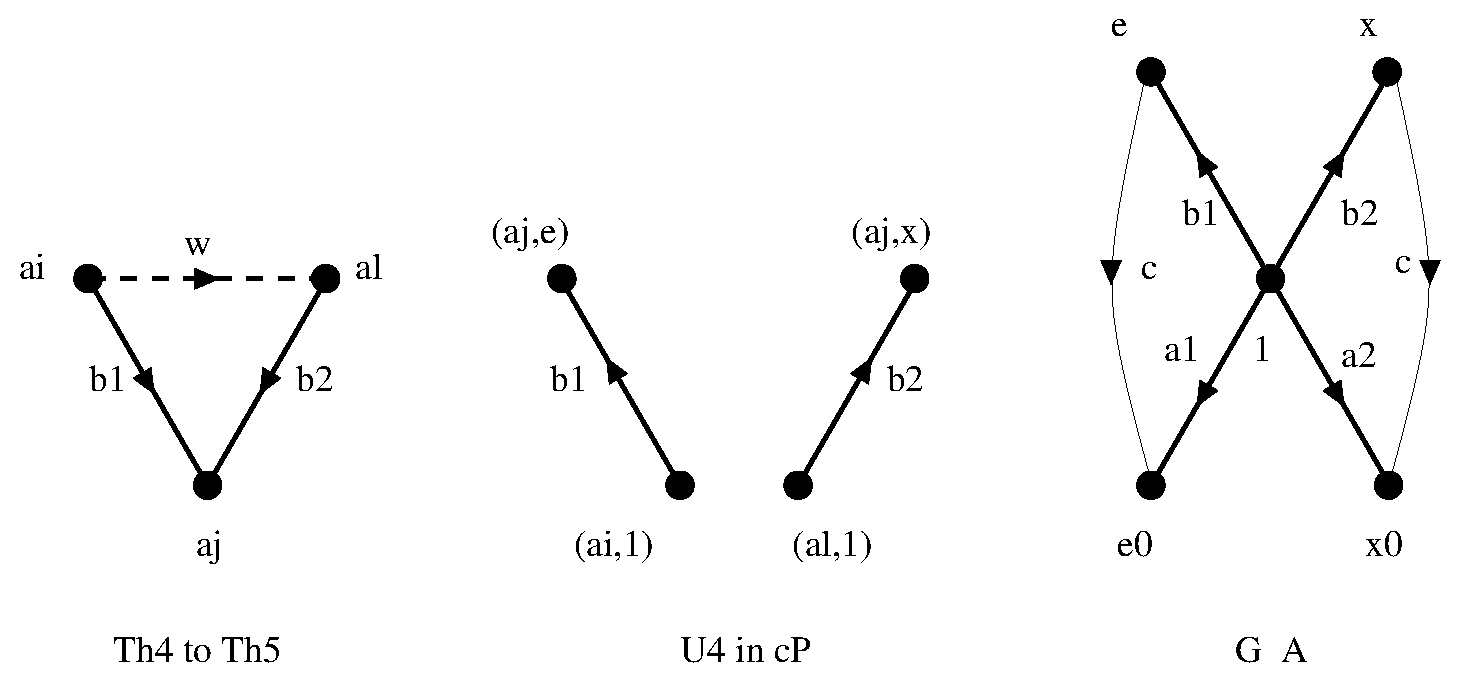
\includegraphics[scale=.5]{alg2-5.eps}
\end{center}
\caption{$\Theta_4$ to $\Theta_5$:
$w=\phi_k^{-1}(t_1ca_1^{-1})a_1a_2^{-1}\phi_k^{-1}(a_2c^{-1}t_2^{-1})$.}
\label{fig:alg2-5}
\end{figure}

Repeat this process for all such pairs $(\e_1,\e_2)$ 
and all such paths $p_1$ and $p_2$.
To see that the image of the language accepted by
 the new graph is the same as that of the original note
that the word $t_1t_2^{-1}$ is readable, starting at $\a_1$ and
ending at $\a_2$, in $\T_4$. As $\pi(t_1t_2^{-1})=\pi(w_1a_1a_2^{-1}w_2^{-1})$
the addition of this new path has no effect on the image, under $\pi$, of
the language accepted by the automaton.

 Fold the resulting graph to form $\T_5$. As before, there is
a natural morphism $\theta_5$ from $\Theta_4$ to $\Theta_5$ and again,
if $\a,\b$ are
vertices of $\Theta_4$ and $L_4$ and $L_5$ are the languages accepted by
$(\Theta_4,\a,\b)$ and $(\Theta_5,\theta_4(\a),\theta_4(\b))$,
respectively, then $\pi(L_4)=\pi(L_5)$.

(There is alot of redundancy built in to this modification step. In 
Example \ref{ex:K} below we discuss how to avoid some of the unnecessary
 work.)\\[1em]


\noindent\textbf{Reassembly.}\\
The modification process is applied to all $X_k$ components of $\D_k$,
for $k=1$ and $2$. Roughly speaking a new graph is then constructed by
reconnecting the modified $X_k$ components in the same way as they
were connected in $\D$. In detail,
let $\cC$ be the set of all
$X_1$ and $X_2$ components.
Define
\[E_Z=E(\D)\bs \cup_{\Phi\in \cC} E(\Phi)\]
and $\D_Z$ to be the subgraph of $\D$ consisting of all edges
of $E_Z$, and their incident vertices.
Define $\D^\prime$ to be the disjoint union of the
 graphs $\T$, such that $\T\in \cC$, with  the graph $\D_Z$.
Also define $\D^{\prime}_5$ to be the disjoint union of the graphs
$\T_5$, such that $\T\in \cC$, with the graph $\D_Z$. For each
$\T\in \cC$ there is  a morphism
$\theta_5\circ\theta_4\circ\theta_3\circ\theta_2\circ\theta_1$
from $\T$ to $\T_5$. Define $\theta$ to be the morphism from
$\D^\prime$ to $\D^\prime_5$ which consists of the union of these
morphisms with the identity morphism of $\D_Z$. By
construction, for each connected component $\Xi$ of $\D^\prime$
there is an embedding of $\Xi$ into $\D$. Let $\nu$ be the union
of these embeddings over all components of $\D^\prime$.

%\noindent\textbf{Output of Algorithm II.}\\
The output of Algorithm II is the quotient $\D''$ of
 $\D^\prime_5$ defined as follows.
Let $u$ and $v$ be vertices
 of $\D^\prime_5$.
\be[R1]
\item\label{it:R1} If $\nu(\theta^{-1}(u))\cap \nu(\theta^{-1}(v))\neq \nul$ then
identify vertices $u$ and $v$.
For $u \in V(\D^\prime_5)$ let
$[u]$  denote equivalence class of $u$ under the equivalence relation $\approx$ 
on $V(\D^\prime_5)$ generated by this identification.
\item
$\D^{\prime\prime}$ has edge set
\[\{([u],a,[v]): (u,a,v)\in E(\D^\prime_5)\}.\]
\item The root vertex of $\D^{\prime\prime}$ is the image, in
$\D^{\prime\prime}$, of $\nu^{-1}(1)$, where $1$ is  the root of
$\D$.
\ee
In order to compute $\D''$, at each stage of the modification process
we record the inverse images of vertices, under the maps $\theta_i$: these are the
sets denoted $\vim$ in the summary of Algorithm II in Section \ref{sub:summaryII}.

\begin{lemma}\label{lem:resol-quot}
Let $[\cdot]$ be the equivalence relation on $V(\D^\prime_5)$
described above. There is a morphism $\rho$ from  $\D$ to
$\D^{\prime\prime}$ given by
\begin{itemize}
\item
$\rho(u)=[\theta(\nu^{-1}(u))]$, for
$u\in V(\D)$, and
\item
$\rho((u,a,v))=(\rho(u),a,\rho(v))$, for $(u,a,v)\in  E(\D)$.
\end{itemize}
\end{lemma}
\begin{proof}
First $\rho$ must be shown to be well defined.
That is, we must verify that $[\theta(\nu^{-1}(u))]$ is a vertex of
$\D^{\prime\prime}$ and that $[\rho(u),a,\rho(v)]$ is an edge.
If $u \in V(\D)$
then either $u\in V(\D_Z)$ or  $u$ belongs to
some $X_k$ component of $\D$. Hence
 $\nu^{-1}(u)\neq \nul$. If $u_1, u_2\in \nu^{-1}(u)$, then,
by definition of
$\D^{\prime\prime}$, $\theta(u_1)$ and $\theta(u_2)$ are equivalent.
Thus $[\theta(\nu^{-1}(u)]$ is a vertex of $\D^{\prime\prime}$,
as required.
 Suppose that $(u,a,v)$ is an edge
of $\D$ and let $u_1\in \nu^{-1}(u)$ and $v_1\in \nu^{-1}(v)$. Then
$\rho(u)=[\theta(u_1)]$ and $\rho(v)=[\theta(v_1)]$, so
$[\rho(u), a, \rho(v)]$ is an edge of $\D^{\prime\prime}$.
Hence $\rho$ is well-defined, and is, moreover, a graph morphism.
\end{proof}


\begin{definition}
Let $\D$ be an inverse automaton.
%, with alphabet $\S$ and
%start and final state $1$, such that
%$\pi(L(\D))=K$.
 The result $\D^{\prime\prime}$ of applying  \ref{it:gf1}
above to $\D$ is called a \emph{double coset resolution} or
\emph{dc-resolution} of $\D$. The graph $\Psi$ obtained by applying
 \ref{it:gf2} to $\D^{\prime\prime}$ is called a \emph{double
coset folding} or \emph{dc-folding} of $\D$.  The composition $\hat\rho$ of
the  morphism
$\rho:\D\maps \D^{\prime\prime}$ with the folding morphism $\D^{\prime\prime}\maps
\Psi$ is called the \emph{dc-folding morphism}.
\end{definition}
\section{Summary of the generalised folding algorithm}
In this section we summarise the algorithms which we have described above,
in a form suitable for the analysis of their complexity,
in Section \ref{sec:TC} below. That is we summarise Algorithms I and II
and the Generalised Folding Loop of Section \ref{sec:dca}. The Generalised Folding Loop, which calls Algorithm II
during its execution, is what we refer to as the ``Generalised Folding
Algorithm''.
\subsection{Summary of algorithm I}\label{sub:sum_algI}
\subsubsection{Preproccessing.}
Given $F_1*_{H_1=H_2} F_2$
 the
steps in this subsection are carried out once for
each group $H_i$. Once these steps have been completed
then execution of Algorithm I of Section \ref{sub:alg1ex} can be carried out as many times as necessary,
to find double coset normal forms.

\noindent\textbf{Input.}
\biz
\item generators $X$ of a free group $\FF(X)$.
\item A finite set $Y$ of elements of $\FF(X)$.
\eiz
\noindent\textbf{Output.}
\biz
\item
$\G_A$, the Stallings automaton for the subgroup $H=\la Y\ra$ of $\FF(X)$.
\item
$L_T$, the set of words corresponding to a  maximal subtree $T$ of $\G_A$.
\item The set $P$ of non-diagonal elements of $V( \G_A\times \G_A)$
partitioned into equivalence classes of $\sim$ (i.e. vertices in the
same connected components of $\G_A\times \G_A$).
\item $P_0$ the set of representatives of equivalence classes of
elements of $P$.
\item $C$ the set of connecting elements, one for each element of $P$.
\eiz
\noindent\textbf{Process.}
Let $N=\sum_{y\in Y} |y|$.
\be[{A}1]
\item Construct $\G_A$.
\begin{comp}
($t_1(N)$.)
\end{comp}
\item Construct a spanning tree $T$ for $\G_A$ and simultaneously
compute $L_T=L_T(A)$.
\begin{comp}
(This can easily be done if $T$ is constructed by
BFS or DFS, so one problem I was worrying about disappears.) ($O(N^2)$.)
\end{comp}
\item Construct $\G_A\times \G_A$.
\begin{comp}
($t_3(N,N)$).
\end{comp}
\item Find connected components of $\G_A\times \G_A$. This can be
done by doing a BFS or DFS of $\G_A\times \G_A$, which constructs
a spanning forest $F$ at the same time as finding the set $C$ of
connecting elements,
which can be taken to be labels of paths in the spanning forest $F$.
\begin{comp}
($O(N^4)$).
\end{comp}
\item Construct the set $P_0$. This can be done using $L_T$ and
the forest $F$.
\begin{comp}
($O(N^2)$).
\end{comp}
\ee
\begin{comp}\noindent\textbf{Question.} Is it better for our algorithm
to construct $T$ by BFS or DFS? Does it make any difference to the
Algorithm II?
\end{comp}

\begin{comp}
Preprocessing time is bounded above by $O(N^4)$.
\end{comp}
\subsubsection{Execution of Algorithm I}\label{sub:alg1ex}
\noindent\textbf{Input.}
\biz
\item $w$, a reduced word in $\FF(X)$.
\eiz
\noindent\textbf{Output.}
\biz
\item The double coset normal form of $w$, as an ordered triple
$(h,s,h')$, where $h,h'\in H$ and $s$ is a double coset representative
of $H$.
\eiz
\noindent\textbf{Process.}
\be[{B}1]
\item Find the maximal prefix $h$ of $w$ accepted by $\G_A$.
Let $w=h\circ f$.
\item If $h=w$ then output $(w,1,1)$ and stop. 
\item Use $\G_A$ to find the maximal $L_Q$-prefix $p$ of $f$.
Let $f=p\circ q$.
\item Find the maximal prefix $g$ of $q^{-1}$ accepted by $\G_A$.
Let $q=r^{-1}\circ g^{-1}$.
\item Use $\G_A$ to find the maximal $L_Q$-prefix $t$ of $r$.
Let $r=t\circ e^{-1}$.
\item If $e=1$ go to step \ref{it:ss}.
\item Using $L_T$, set $y=w(\t(p))$ and $z=w(\t(t))$.
\item Freely reduce $hpy^{-1}$, $yez^{-1}$ and $zt^{-1}g^{-1}$ and
call the results   $a, b$ and $c$, respectively.
\item Output $(a,b,c)$ and stop.
\item\label{it:ss} (This step is reached only if $e= 1$.)
 Using $P_0$ and $F$ find the representative $(u_0,v_0)$ of $(u,v)$, where
$u=\t(p)$ and $v=\t(t)$.
\item Look up the connecting element $c=c(u,v)$.
\item Let $y=w(u_0)$ and $z=w(v_0)$.
\item Freely reduce $hpcy^{-1}$ and $zc^{-1}t^{-1}g^{-1}$ and call the
results $a$ and $b$, respectively.
\item Output $(a,yz^{-1},b)$.
\ee

\begin{comp}
The time required for these steps is $O(|w|)$.
\end{comp}
\subsection{Summary of Algorithm II}\label{sub:summaryII}

Here we assume $F_1*_{H_1=H_2} F_2$
 where $F_k$ is generated by $X_k$, $H_k$ is generated
by $Y_k=\{h_{k,1},\ldots, h_{k,m}\}$
and the Stallings automata $\G_{A_k}$ for $H_k$ have
been constructed, for $k=1,2$. Let  $\S=(X_1\cup X_2\cup Z)^{\pm 1}$ and, for $k=1,2$,
assume that we have constructed, at the preprocessing stage, the following.
\be
\item
A spanning tree  $T_k$ for $\G_{A_k}$,
 the set $L_{T_k}$of words corresponding to the  maximal subtree $T_k$,
the set $P_k$ of non-diagonal elements of
$V( \G_{A_k}\times \G_{A_k})$,
 the set $P_{k,0}$ of representatives  of equivalence classes of
elements of $P_k$ and the
set $C_k$ of connecting elements, one for each element of $P_k$.
%%%%%%%%
\item A map $\phi_k:Z\maps F_k$  inducing an isomorphism from $\FF(Z)$ to
$H_k$. This map is encoded as part of $\G_{A_k}$. More precisely,
edges of $\G_{A_k}$ have two types of label; \emph{input} and \emph{output}.
Labels discussed above are input labels, are
referred to simply as \emph{labels}, and are elements of $X_1\cup X_2$.
\emph{Output labels} are elements of  $Z\cup \{1\}$.
 Edges of $T_k$  all have output label $1$; and each directed
edge of $\G_{A_k}$ not in $T_k$ has output
label an element of $Z$. Each such edge corresponds uniquely to
 an element $h_{k,i}$ of the free generating set for $H_k$, and the edge
corresponding to $h_{k,i}$ has
 output label  $z_i\in Z$. Moreover, in this case $\phi_k(z_i)=h_{k,i}$.
  This means that if a word in $H_k$ is given in terms of $Y_k$  then its
image under $\phi_k^{-1}$ can be read off from $\G_{A_k}$ (regarded as a
 transducer), by reading output labels.
\ee

\noindent\textbf{Input.}
\biz
\item An inverse automaton $\D$ with alphabet $\Sigma$ and start
and final state $1$, such that $\pi(L(\D))=K$. Edges labelled
with elements of $X_k$ are said to have type $k$. Edges labelled with
elements of $Z$ are said to have type $Z$.
\item Stallings automata $\G_{A_1}$ and $\G_{A_2}$ for $H_1$ and $H_2$,
with output labels
encoding $\phi_1$ and $\phi_2$, as above.
\item For each $z \in Z$ the images $\phi_1(z)$ and $\phi_2(z)$ of
as words in $Y_1^{\pm 1}$ and $Y_2^{\pm 1}$, respectively.
\eiz
\noindent\textbf{Output.}
\biz
\item An inverse automaton $\D''$ (with alphabet $\Sigma$ and start
and final state $1$, such that $\pi(L(\D''))=K$).
\eiz
\noindent\textbf{Process.}\\
Each of the following steps is executed for $k=1$ and $2$.
\be[{C}1]
\item\label{it:C1} Construct $\D_{k,0}$ and  
a set $\vim(\a)$, for each vertex  $\a$ of $D_{k,0}$. These
sets will be updated at each stage of the algorithm and will eventually
equal the sets $\nu\theta^{-1}(v)$, for vertices of $\D'_5$.  In detail the steps are
the following.
\be
\item\label{it:C1a} Remove all edges of type $X_{k'}$, where $k'=3-k$, from $\D$ to give a graph $\D'_{k,0}$.
\item\label{it:C1b} A \emph{shoot} is an edge incident to a leaf. Remove all shoots
of type $Z$ from $\D'_{k,0}$; adding
edges removed to  a graph $\D_Z$ (which starts off empty, when $k=1$, and 
is not reinitialised when $k$ is incremented to $2$). Continue
until there are no shoots of type $Z$ in $\D'_{k,0}$. The resulting graph
is $\D_{k,0}$. 
\item\label{it:C1c} Rename vertices of $\D_{k,0}$: 
a vertex named $v$ in $\D$ becomes
$(v,k)$ in $\D_{k,0}$.
\item\label{it:C1d} For each vertex $(v,k)$ of $\D_{k,0}$,  set 
  $\vim(v,k)$ equal to $\{v\}$.  For each vertex $v$ of $\D_Z$, 
set $\vim(v)=\{v\}$. 
\ee
\item\label{it:C2} (\textbf{Begin Modification 1}.) For all edges
$(\a,z,\b)$ of $\D_{k,0}$, where $z\in Z$, add a path $(\a,\phi_k(z),\b)$ to
$\D_{k,0}$. The resulting graph is called $\D_{k,1}'$. 
For each vertex $(v,k)$ in $V(\D_{k,1}')\backslash V(\D_{k,0})$ set 
$\vim(v,k)=\{v\}$. 
\item\label{it:C3} Construct the Stallings folding$\D_{k,1}$  of (each component of)
$\D_{k,1}'$.  
Whenever two vertices $(u,k)$ and $(v,k)$
of $\D_{k,1}'$ are identified, by the folding map, to a vertex $(w,k)$, 
set $\vim(w,k)=\vim(u,k)\cup \vim(v,k)$. 
The sets $\vim(u,k)$ and $\vim(v,k)$ may be deleted.  This process, combined 
with the initialisation, above, of $\vim$ (to a single vertex) for new vertices
added,  will be
called \emph{updating}
$\vim$, from now on. 
\item\label{it:C4} (\textbf{Begin Modification 2}.)
 Construct $\cP_{k,1}=\D_{k,1}\times \G_{A_k}$.
\item\label{it:C5} Construct a spanning forest $\U_{k,1}$ of $\cP_{k,1}$.
\begin{comment} and, 
simultaneously,
the set $L_{\U_k}$ of words corresponding to paths in $\U_k$ from the root
to each vertex. (A root of $\cP_k$ must  be chosen:
 to be explicit, assume the root is
 $((v,k), u)$, where
$u$ is minimal in some preassigned order on vertices of $\G_{A_k}$ and
$v$ is minimal in some chosen order of vertices of $\D$.)
 We refer to these versions of $\cP_k$ and $\U_k$ as
$\cP_{k,2}$ and $\U_{k,2}$ in the calculation of complexity below.
\end{comment}
\item\label{it:C6} For each vertex $\a$ of $\D_{k,1}$ do the following.
 Let
$\theta(\a)$ be the component of $\cP_{k,1}$ containing $(\a,1)$.
For each vertex $(\b,1)$ of $\theta(\a)$ and for all paths $p$ from
$(\a,1)$ to $(\b,1)$, which do not contain  any vertex $(\g,1)$ other than
the end points, 
 add a path from $\a$ to $\b$ to the graph $\D_{k,1}$, with
label $\phi_k^{-1}(w)$, where $w$ is the label of $p$.
The resulting graph is called $\D_{k,2}'$.
\item\label{it:C7} Construct the Stallings folding $\D_{k,2}$ of $\D'_{k,2}$ and update $\vim$.
\item\label{it:C8} (\textbf{Begin Modification 3}.)
 Construct $\cP_{k,2}=\D_{k,2}\times \G_{A_k}$ and its spanning
 forest $\U_{k,2}$, by adding new isolated vertices to $\cP_{k,1}$ and 
$\U_{k,1}$,
if necessary. 
\item\label{it:C9} For all vertices of $\cP_{k,2}$ of the 
form $(\a,1)$ do the following.
Let $\theta(\a)$ be the component of $\cP_{k,2}$ containing $(\a,1)$.
For each edge $e$ of $\theta(\a)\bs \U_{k,2}$: 
if $e=((\a_i,\b_1),x ,(\a_j,\b_2))$,
where $\a_i,\a_j$ are vertices of $\D_{k,2}$ and $\b_1,\b_2$ are vertices
of $\G_{A_k}$ and $x\in X_k$, add to $\D_{k,2}$ a path from $\a$ to $\a$ with
label $\phi_k^{-1}(l_ixl_j)$, where $l_i$ and $l_j$ are the labels of
paths in $\U_{k,2}$ from $(\a,1)$ to $(\a_i,\b_1)$ and from $(a_j,\b_2)$ 
to $(\a,1)$,
respectively. The resulting graph is called  $\D_{k,3}'$.
\item\label{it:C10} Construct the Stallings folding $\D_{k,3}$ of 
$\D'_{k,3}$ and update $\vim$.
\item\label{it:C11} (\textbf{Begin Modification 4}.)
 Construct  $\cP_{k,3}=\D_{k,3}\times \G_{A_k}$ and its spanning
 forest $\U_{k,3}$, by adding new isolated vertices to $\cP_{k,2}$ and 
$\U_{k,2}$,
if necessary. 
\item\label{it:C12} For all vertices of $\cP_{k,3}$ of the 
form $(\a,1)$ do the following.
Let $\theta(\a)$ be the component of $\cP_{k,3}$ containing $(\a,1)$.
For all vertices $(\a_1,\b)$ of $\theta(\a)$, with $\b\neq 1$, let
$b=w(\b)$, the label of the path from $1$ to $\b$ in $T_k$. If
$b$ is readable in the automaton $\cP_{k,3}$ with start state $(\a,1)$ and
the final state, after reading $b$, is $(\a_1,\b)$ there is nothing to do,
for this vertex $(\a_1,\b)$. Otherwise, let $a$ be the label of the
path from $(\a,1)$ to $(\a_1,\b)$ in $\U_{k,3}$. Add to $\D_{k,3}$ a path from
$\a$ to $\a_1$ with label $(\phi_k^{-1}(ab^{-1}))b$.
The resulting graph is called $\D_{k,4}'$.
\item\label{it:C13} Construct the Stallings folding $\D_{k,4}$ of $\D'_{k,4}$ 
and update $\vim$.
\item\label{it:C14} (\textbf{Begin Modification 5}.)
Construct  $\cP_{k,4}=\D_{k,4}\times \G_{A_k}$ and its spanning
 forest $\U_{k,4}$. 

\item\label{it:C15}   For each element $(\e_1,\e_2)\in P$ and
each vertex $\b\in V(\D_{k,4})$ 
such that $\vim(\b)\cap V(\D')\neq \emptyset$, do the following. 
Let $C_1$ and $C_2$ be the components of $\cP_{k,4}$ containing 
$(\b,\e_1)$ and $(\b,\e_2)$, respectively. Assume that there are vertices
$\a_1$ and $\a_2$ of $\D_{k,4}$ such that $\vim(\a_i)\cap V(\D')\neq \emptyset$ and 
$(\a_i,1)\in V(C_i)$, for $i=1$ and $2$. (If any of these  conditions fail 
 there
is no action to be taken for this $\b$.) Let $t_i$ be the label
of the path from $(\a_i,1)$ to $(\b,\e_i)$, in $\U_{k,4}$.  Let 
$(\xi_1,\xi_2)$ be  the $\sim$ representative of $(\e_1,\e_2)$, let 
$c=c(\e_1,\e_2)$ be the connecting element of $(\e_1,\e_2)$ and 
let $a_i=w(\xi_i)$, $i=1,2$. Add  a path to $\D_{k,4}$, 
from $\a_1$ to $\a_2$, with label
$\phi_k^{-1}(t_1ca_1^{-1})a_1a_2^{-1}[\phi_k^{-1}(t_2ca_2^{-1})]^{-1}$. 
The resulting graph is called  $\D_{k,5}'$.
\item\label{it:C16} Construct the Stallings folding $\D_{k,5}$ of $\D'_{k,5}$ 
and update $\vim$.
\item\label{it:C16.5} Set $\D'_5$ equal to the disjoint union
$\D_{1,5}\cup \D_{2,5}\cup \D_Z$. 
\item\label{it:C17} (\textbf{Begin Reassembly}.) 
For each vertex $(u,k)$ of $\D_{1,5}\cup \D_{2,5}$,
do the following. For each vertex $(v,k')$ of $\D_{1,5}\cup \D_{2,5}$, not
equal to $(u,k)$, if
$\vim((u,k))\cap \vim((v,k'))\neq \emptyset$ then replace  
$\vim((u,k))$ with $\vim((u,k))\cup
\vim((v,k'))$. In this case, for each edge $e$ of $\D_{1,5}\cup \D_{2,5}$, if $e$ has
initial or terminal vertex equal to $(v,k')$ then replace $e$ with
an edge having $(u,k)$ as initial or terminal vertex, instead of $(v,k')$.
Delete $(v,k')$, once no more such edges exist.
Continue for as long as possible: that is until 
$\vim(u,k)\cap \vim(u',k')=\emptyset$, whenever $(u,k)\neq (u',k')$. The resulting graph is denoted $\D''_5$.
\item\label{it:C18} 
If $\vim(\a)\cap \vim(u,k)\neq \nul$,
 for some
 vertices $\a$ of $\D_Z$ and $(u,k)$ of $\D'_5$ then replace $\a$ 
with $(u,k)$ and add $\a$ to $\vim(u,k)$. (Note that, as
we have completed step \ref{it:C17}, there is at most one such vertex of
$\D'_5$.)
If $\a$ has been replaced by $(u,k)$ then, for every edge $e$ of $\D_Z$,
 of the form $(\a,\b)$ (or its reverse), replace $e$ with
 the edge $((u,k), \b)$ (or its reverse). Call the resulting graph $\D_Z''$.
\item\label{it:C19} Form $\D''$ from the union of $\D''_5$ and $\D_Z''$:
 by identifying vertices of $\D_Z''$ with vertices of  $\D''_5$
of the same name.
%\item\label{it:C20}  Construct $\D''$, the Stallings folding of $\bar \D$.
\ee
In Lemma \ref{lem:idverts} below we verify that the graph output from 
Step \ref{it:C19} is the same as the graph $\D''$ constructed in Section
\ref{sec:dca}, using the equivalence relation $\approx$.  

\subsection{Summary of the Generalised Folding Loop}
Here the assumptions are as for Algorithim II.

\noindent\textbf{Input.}
\biz
\item A tuple $k_1, \ldots ,k_s$ of elements of $F_1*_{H_1=H_2}F_2$,
in double coset normal form.
% and the Stallings folding $\G_K$ of this
%tuple as a set of words in $F_1*F_2*\FF(Z)$.
\eiz
\noindent\textbf{Output.}
\biz
\item An inverse automaton $\Psi$, with alphabet $\Sigma$ and start
and final state $1$, such that $\pi(L(\Psi))=K$ and $\Psi$ accepts the
double coset normal form of every element of $K$.
\eiz
\noindent\textbf{Process.}\\
\be[{D}1]
\item Form the flower automaton $\cF(K)$ of the subgroup $\hat K$ of 
$\FF(X_1\cup X_2\cup Z)$ generated by $k_1,\ldots, k_s$, as in Section 
\ref{sec:dca}. 
\item Construct the Stallings folding $\G_K$ of $\cF(K)$. 
\item Set $n=0$ and $\D_{(0)}=\G_K$.
\item\label{it:loop2} Input $\D_{(n)}$ to Algorithm II.
Call the output $\D''_{(n+1)}$.
\item\label{it:loop3} Fold  $\D''_{(n+1)}$ and call the result   $\D_{(n+1)}$.
\item If the number of $X_1$ and $X_2$ components of $\D_{(n)}$ and
$\D_{(n+1)}$ are the same, output $\D_{(n+1)}$ and halt. Otherwise,
 add $1$ to $n$ and go to Step \ref{it:loop2}.
\ee
\subsection{Generalised folding example}
\begin{example}\label{ex:K}
Let $F_1=\FF(x_1,x_2,x_3)$ and $H_1=\la h_1,h_2,h_3\ra$,
as in Example \ref{ex:f_1}, and let $F_2=\FF(y_1,y_2,y_3,y_4)$ and
$H_2=\la h_1^\prime, h_2^\prime, h_3^\prime\ra$, as in Example \ref{ex:f_2}.
Let $f_1,f_2$ and $f_1^\prime$ be the elements defined in these examples
 and let $G=F_1\ast_{H_1=H_2} F_2$.

Let
\[f_3=x_2x_3^{-1}x_1,\, f_4= x_1^4 x_2 x_3 x_1^{-1} x_2^{-1}
\textrm{ and } f_5=x_1x_2x_3x_2x_3^{-2}x_2^{-1},\]
and let
\[ f_2^\prime =y_3y_4y_2^{-1}y_1y_3.\]
Using Algorithm I, the double coset normal forms of these elements are
\begin{align*}
f_3 & = x_2x_3^{-1}x_1,\\
f_4 &= h_1h_3 x_1^{-1}x_2^{-1},\\
f_5 &= h_3h_2^{-2}\textrm{ and }\\
f_2^\prime &= h_2^\prime y_2^{-1}y_1y_3.
\end{align*}

Let $K$ be the subgroup of $G$ generated by $k_1=f_1f_1^\prime f_2$,
$k_2= f_3f_2^\prime f_4$ and $k_3=f_5$.
In Example \ref{ex:g} we found the double coset normal form of
$k_1=g=f_1f_1^\prime f_2$, namely
\[k_1=z_2^2 z_1  x_1 x_3 x_1 z_1^{-1}
z_2y_1y_2^{-1} z_1^{-1}z_2^{-1}
z_3^{-1}z_2^{-1} x_1^{-1}.\]
The double coset normal forms of $k_2$ and $k_3$ are
\[k_2=  x_2x_3^{-1}x_1  z_2 y_2^{-1}y_1y_3 z_1z_3 x_1^{-1}x_2^{-1}\]
and
\[k_3 = z_3z_2^{-2}.\]

We form the flower automaton of $K$ and then its (classical) Stallings folding,
which is
shown in Figure \ref{fig:Kflower}.
There is one $X_1$ component $\Theta$ of this graph, shown in Figure \ref{fig:KX}
and two $X_2$ components, $\Theta^\prime$ and $\Theta^{\prime\prime}$,
shown in Figure \ref{fig:KY}. Thus $\D_{1,0}=\Theta$ and 
$\D_{2,0}=\T'\cup \T''$. Each of these components is input to
 the Generalised Folding Loop, in turn.  The graph $\D_Z$ is shown
in Figure \ref{fig:notyetdrawn}.

First consider the $X_1$ component $\Theta$. Modification 1
results in the graph of Figure \ref{fig:K_f1}. To perform the next
stages of the  modification process the graph  $\cP_{1,1}=\Theta_1 \times
\G_{A_1}$ is constructed; where $\G_{A_1}$ is the graph of Example
\ref{ex:f_1}, shown in Figure \ref{fig:stall1}. The  graph
$\cP_{1,1}$ is shown in Figure \ref{fig:K_f1-x-g}. The spanning forest
chosen for $\cP_{1,1}$ is the one obtained by removing the edge
joining vertices $(13,1)$ and $(30,5)$. On examination of $\cP_{1,1}$
there is one path to add: corresponding to the path in $\cP_{1,1}$,
from $(15,1)$ to $(31,1)$, labelled $x_1^{-3}$. Thus a path is
added to $\T_1$, from the vertex $15$ to the vertex $31$, with
label $z_1^{-1}$. There are no other paths to add which do not
already exist in $\T_1$. The result is  the graph $\D_{1,2}=\Theta_2$,
shown in Figure \ref{fig:K_f2}. 

The next step is to construct
$\cP_{1,2}=\T_2\times \G_{A_1}$, but as there are no $X_1$ edges in
$\T_2$ that are not in $\T_1$, it follows that  $\cP_{1,2}$ is the
union of $\cP_{1,1}$ and some isolated vertices, and we may use
$\cP_{1,1}$ instead of $\cP_{1,2}$. In this instance there is nothing to
add at this stage and $\D_{1,3}=\T_3=\T_2$.

In formation of $\D_{1,4}=\T_4$ paths are added to $\T_3$,
corresponding to pairs of vertices $(\g,\d)$ of $\cP_{1,3}$ (which 
is the union of $\cP_{1,1}$ with some isolated vertices), that 
are not covered by $\cP_{1,3}$.
In the table of Figure \ref{tab:T4} the paths to be added are listed:
each row corresponds to such a pair $(\g,\d)$. The
label of the path from $\g=(\a_i,1)$ to $\d=(\a_j,\b)$
in $\cP_{1,3}$ is $a$,
the label of the path from $1$ to $\b$ in $\T_k$ is $b$, and the word
$\phi_k^{-1}(ab^{-1})$ is $w$. For each line of the table a path,
from $\a_i$ to $\a_j$, with label $wb$, is added to $\T_3$.
(These are not the only pairs of vertices which are not
covered: however, the other pairs do not result in any further paths
being added.)
\begin{figure}
\begin{center}
\renewcommand{\arraystretch}{1.5}
\begin{tabular}{|c|c|c|c|c|}
\hline
$\g$& $\d$ & $a$ & $b$ & $w$\\\hline\hline
$(25,1)$ & $(13,5)$ & $x_2x_3$ & $x_2$ & $z_2 $\\\hline
$(29,1)$ & $(25,2)$ & $x_3^{-1}x_2^{-1}x_1$ & $x_1^{-1}$ & $z_3^{-1}z_1$\\\hline
$(32,1)$ & $(15,2)$ & $x_1^2$ & $ x_1^{-1}$ & $z_1$\\\hline
$(32,1)$ & $(13,3)$ & $x_1^{-2} $ & $x_1 $ & $z_1^{-1} $\\\hline
$(32,1)$ & $(30,4)$ & $x_1^{-2}x_2$ & $x_3^{-1} $ & $z_1^{-1}z_3$\\\hline
$(1,1)$ & $(3,5)$ & $x_2x_3^{-1} $ & $x_2 $ & $z_2^{-1} $\\\hline
$(30,1)$ & $(12,3)$ & $x_3^{-1}x_2^{-1}$ & $x_1 $ & $z_3^{-1} $\\\hline
$(29,1)$ & $(1,3)$ & $x_3^{-1}x_2^{-1}$ & $x_1 $ & $z_3^{-1} $\\\hline
\end{tabular}
\renewcommand{\arraystretch}{1}
\end{center}
\caption{Paths to be added to form $\T_4$}
\label{tab:T4}
\end{figure}
After adding these paths to $\T_3$ the graph is folded to
produce the graph $\T_4$, shown in Figure \ref{fig:K_f4}.

To form $\D_{1,5}=\T_5$ we first construct $\cP_{1,4}=\T_4\times \G_{A_k}$,
which is shown in Figure \ref{fig:K_f4-x-g}, and choose a spanning
subforest $\U_4$ of $\cP_{1,4}$. In this example this is done by
removing the edge  joining vertices $(13,1)$ and $(30,5)$ from
$\cP_{1,4}$. A path will be added to $\T_4$ whenever a pair $(\e,\xi)$
in the set $P$ of non-diagonal pairs of vertices of $\G_{A_k}$ is
found, satisfying the conditions given in Modification 5: namely
that
\begin{itemize}
\item
$(\e,\xi)$ is not a $\sim$ representative;
\item  there are paths $p_1$ and $p_2$ in $\U_4$ from
vertices $(\a_i,1)$ to $(\b,\e)$ and from $(\a_j,1)$ to $(\b,\xi)$, for some $\a_i, \a_j, \b\in V(\T_4)$,
and
\item
the labels of $p_1$ and $p_2$  are the same as the labels of the paths, from $1$ to $\e$, and $1$ to $\xi$,
respectively, in $T_k$.
\end{itemize}
If  such a pair $(\e,\xi)$ is found then let $(\e_0,\xi_0)$ be its $\sim$ representative, let
$c$ be the connecting element and let $a_1$ and $a_2$ be the labels of  the paths, from
$1$ to $\e_0$, and $1$ to $\xi_0$, in $T_k$. Then the label of any corresponding  path added to
$\T_4$ is $w=\phi_k^{-1}(b_1ca_1^{-1})a_1a_2^{-1}\phi_k^{-1}(a_2cb_2^{-1})$.
The table of Figure \ref{tab:T5} shows pairs of vertices $(\a_i,1)$, $(\b,\e)$ and $(a_l,1)$, $(\b,\xi)$,
of $\cP_{1,4}$, for which the conditions above are satisfied.
\begin{figure}
\begin{center}
\renewcommand{\arraystretch}{1.5}
\begin{tabular}{|c|c||c|c|}
\hline
$(\a_i,1)$& $(\b,\e)$ & $(\a_l,1)$ & $(\b,\xi)$ \\\hline\hline
$(2,1)$ & $(3,4)$ & $(43,1)$ & $(3,5)$ \\\hline
$(13,1)$ & $(34,4)$ & $(25,1)$ & $(34,5)$ \\\hline
$(14,1)$ & $(32,2)$ & $(31,1)$ & $(32,3)$ \\\hline
$(15,1)$ & $(14,2)$ & $(32,1)$ & $(14,3)$ \\\hline
$(25,1)$ & $(1,2)$ & $(36,1)$ & $(1,3)$ \\\hline
$(31,1)$ & $(13,2)$ & $(40,1)$ & $(13,3)$ \\\hline
\end{tabular}
\renewcommand{\arraystretch}{1}
\end{center}
\caption{Paths to be added to form $\T_5$}
\label{tab:T5}
\end{figure}
In each
case the new path is from $\a_i$ to $\a_l$. There are only
 two pairs  $(\e,\xi)$ which arise: namely $(4,5)$ and $(2,3)$, and the labels of the new paths
added  are $z_3^{-1}x_1$ and $z_1x_1$, respectively. After adding these paths to $\T_4$ the graph is folded to
produce the graph $\T_5$, shown in Figure \ref{fig:K_f5}.


Next consider the $X_2$ component $\T^\prime$. There is nothing to
add to form $\T^\prime_1$. The graph $\cP_1^\prime=\T_1^\prime
\times \G_{A_2}$ is shown in Figure \ref{fig:K_i1-x-g}. There is
nothing to add at the next two  stages so
$\T_1^\prime=\T_2^\prime=\T_3^\prime$, so
$\cP_3^\prime=\cP_1^\prime$. There is one pair of vertices not
covered by $\cP_3$: namely $\g=(6,1)$ and $\d=(5,6)$. Thus a path
is added to $\T_3^\prime$, from $6$ to $5$, with label
$z_1y_2^{-1}$, as shown in Figure \ref{fig:K_i4}. The graph
 $\cP_4^\prime=\T_4^\prime \times \G_{A_2}$ is shown in Figure \ref{fig:K_i4-x-g}. The paths
from $(5,1)$ to $(7,5)$ and from $(6,1)$ to $(7,3)$, in $\cP_4$, give rise to a path to be
added to $\T_4^\prime$. However this path has label $y_2z_1^{-1}$, and joins $5$ to $6$, so already
belongs to $\T_4^\prime$. Hence $\T_4^\prime=\T_5^\prime$.

Finally consider the $X_2$ component $\T^{\prime\prime}$. A similar analysis, details of which
are omitted, shows that $ \T^{\prime\prime}_5$ is the graph shown in Figure \ref{fig:K_j4}.
\begin{comment}
As before $\T^{\prime\prime}=\T^{\prime\prime}_1$ and
$\cP_1^{\prime\prime}$ is shown in Figure \ref{fig:K_j1-x-g}. Again,
$\T^{\prime\prime}_1=\T^{\prime\prime}_2=\T^{\prime\prime}_3$ and $\cP_4^{\prime\prime}$ is
shown in Figure \ref{fig:K_j4-x-g}.
\end{comment}


The folding of the reassembled graph $\Psi$ is shown in  Figure
\ref{fig:out}.  As this graph has the same number of $X_1$ and $X_2$ components as the original,
the algorithm halts after one iteration of the Generalised Folding Loop, outputting $\Psi$.

\end{example}
\begin{figure}
\begin{center}
\psfrag{a}{$x_1$}
\psfrag{b}{$x_2$}
\psfrag{c}{$x_3$}
\psfrag{r}{$y_1$}
\psfrag{s}{$y_2$}
\psfrag{t}{$y_3$}
\psfrag{x}{$z_1$}
\psfrag{y}{$z_2$}
\psfrag{z}{$z_3$}
\psfrag{u}{$y_4$}
\psfrag{0}{\hspace{-2pt}\raisebox{-2pt}{\scriptsize $0$}}
\psfrag{1}{\hspace{-2pt}\raisebox{-2pt}{\scriptsize $1$}}
\psfrag{2}{\hspace{-2pt}\raisebox{-2pt}{\scriptsize $2$}}
\psfrag{3}{\hspace{-2pt}\raisebox{-2pt}{\scriptsize $3$}}
\psfrag{4}{\hspace{-2pt}\raisebox{-2pt}{\scriptsize $4$}}
\psfrag{5}{\hspace{-2pt}\raisebox{-2pt}{\scriptsize $5$}}
\psfrag{6}{\hspace{-2pt}\raisebox{-2pt}{\scriptsize $6$}}
\psfrag{7}{\hspace{-2pt}\raisebox{-2pt}{\scriptsize $7$}}
\psfrag{8}{\hspace{-2pt}\raisebox{-2pt}{\scriptsize $8$}}
\psfrag{9}{\hspace{-2pt}\raisebox{-2pt}{\scriptsize $9$}}
\psfrag{10}{\hspace{-2pt}\raisebox{-2pt}{\scriptsize $10$}}
\psfrag{11}{\hspace{-2pt}\raisebox{-2pt}{\scriptsize $11$}}
\psfrag{12}{\hspace{-2pt}\raisebox{-2pt}{\scriptsize $12$}}
\psfrag{13}{\hspace{-2pt}\raisebox{-2pt}{\scriptsize $13$}}
\psfrag{14}{\hspace{-2pt}\raisebox{-2pt}{\scriptsize $14$}}
\psfrag{15}{\hspace{-2pt}\raisebox{-2pt}{\scriptsize $15$}}
\psfrag{16}{\hspace{-2pt}\raisebox{-2pt}{\scriptsize $16$}}
\psfrag{17}{\hspace{-2pt}\raisebox{-2pt}{\scriptsize $17$}}
\psfrag{18}{\hspace{-2pt}\raisebox{-2pt}{\scriptsize $18$}}
\psfrag{19}{\hspace{-2pt}\raisebox{-2pt}{\scriptsize $19$}}
\psfrag{20}{\hspace{-2pt}\raisebox{-2pt}{\scriptsize $20$}}
\psfrag{21}{\hspace{-2pt}\raisebox{-2pt}{\scriptsize $21$}}
\psfrag{22}{\hspace{-2pt}\raisebox{-2pt}{\scriptsize $22$}}
\psfrag{23}{\hspace{-2pt}\raisebox{-2pt}{\scriptsize $23$}}
\psfrag{24}{\hspace{-2pt}\raisebox{-2pt}{\scriptsize $24$}}
\psfrag{25}{\hspace{-2pt}\raisebox{-2pt}{\scriptsize $25$}}
\psfrag{26}{\hspace{-2pt}\raisebox{-2pt}{\scriptsize $26$}}
\psfrag{27}{\hspace{-2pt}\raisebox{-2pt}{\scriptsize $27$}}
\psfrag{28}{\hspace{-2pt}\raisebox{-2pt}{\scriptsize $28$}}
\psfrag{29}{\hspace{-2pt}\raisebox{-2pt}{\scriptsize $29$}}
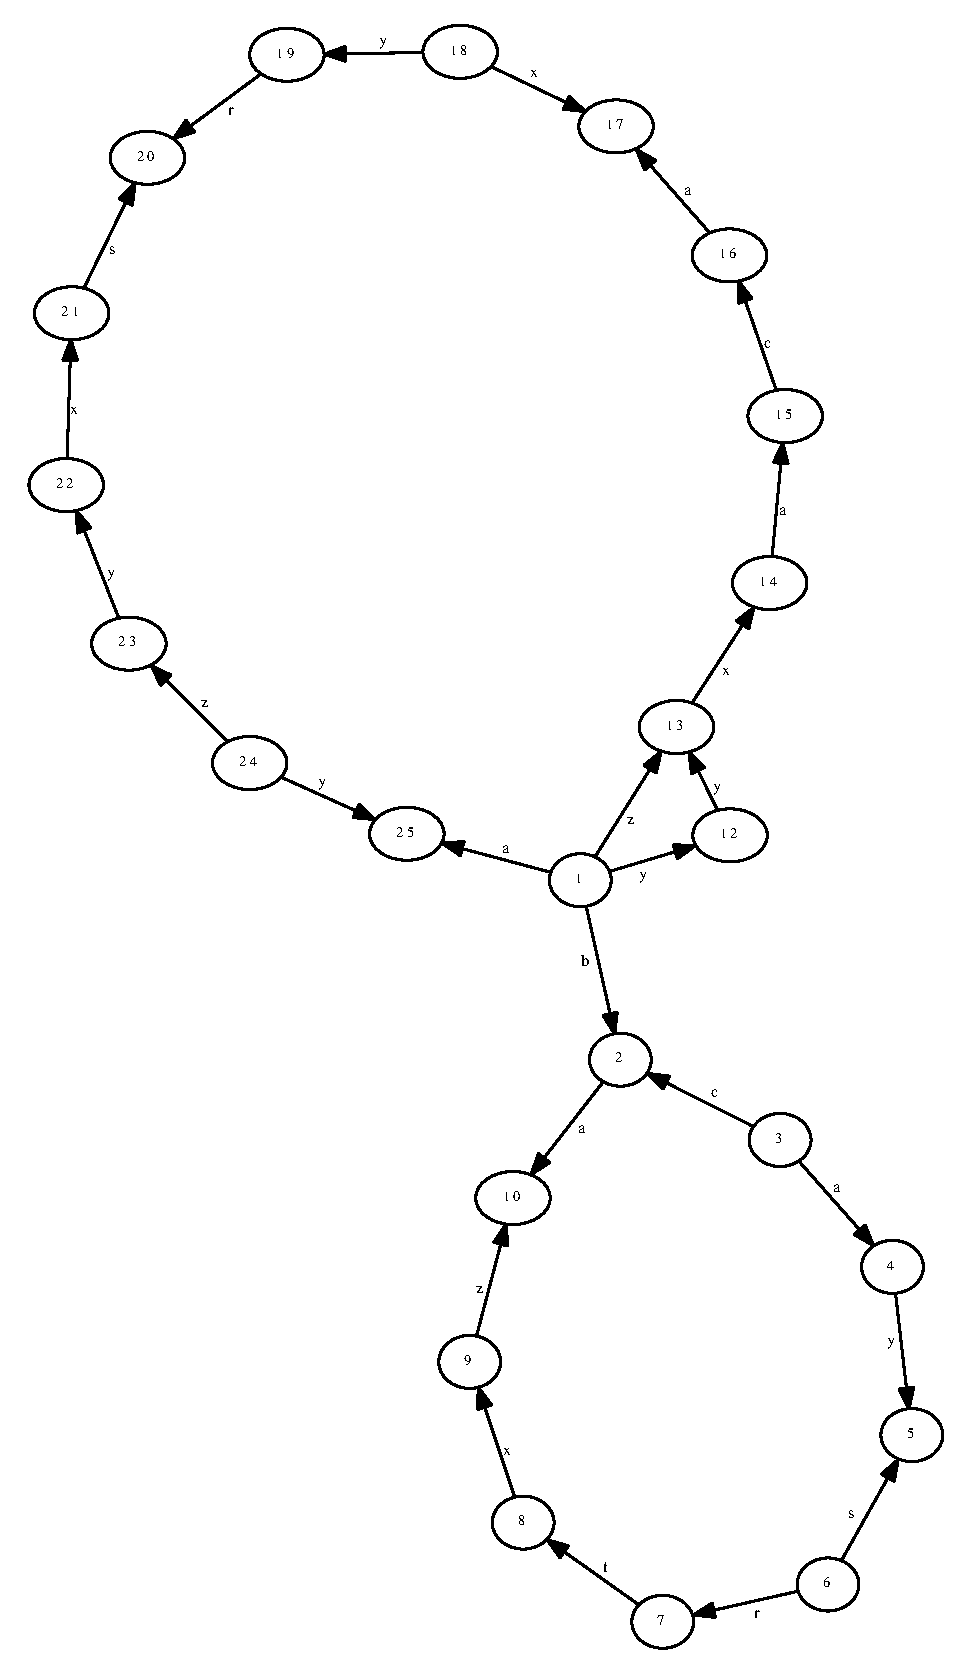
\includegraphics[scale=0.5,bb=0 0 820 720]{python/ex_K_folded.eps}
%\includegraphics[scale=0.4]{python/ex_K.eps}
\caption{The folded flower automaton of $K$}
\label{fig:Kflower}
\end{center}
\end{figure}

\begin{figure}
\begin{center}
\psfrag{a}{$x_1$}
\psfrag{b}{$x_2$}
\psfrag{c}{$x_3$}
\psfrag{r}{$y_1$}
\psfrag{s}{$y_2$}
\psfrag{t}{$y_3$}
\psfrag{x}{$z_1$}
\psfrag{y}{$z_2$}
\psfrag{z}{$z_3$}
\psfrag{u}{$y_4$}
\psfrag{0}{\hspace{-2pt}\raisebox{-2pt}{\scriptsize $0$}}
\psfrag{1}{\hspace{-2pt}\raisebox{-2pt}{\scriptsize $1$}}
\psfrag{2}{\hspace{-2pt}\raisebox{-2pt}{\scriptsize $2$}}
\psfrag{3}{\hspace{-2pt}\raisebox{-2pt}{\scriptsize $3$}}
\psfrag{4}{\hspace{-2pt}\raisebox{-2pt}{\scriptsize $4$}}
\psfrag{5}{\hspace{-2pt}\raisebox{-2pt}{\scriptsize $5$}}
\psfrag{6}{\hspace{-2pt}\raisebox{-2pt}{\scriptsize $6$}}
\psfrag{7}{\hspace{-2pt}\raisebox{-2pt}{\scriptsize $7$}}
\psfrag{8}{\hspace{-2pt}\raisebox{-2pt}{\scriptsize $8$}}
\psfrag{9}{\hspace{-2pt}\raisebox{-2pt}{\scriptsize $9$}}
\psfrag{10}{\hspace{-2pt}\raisebox{-2pt}{\scriptsize $10$}}
\psfrag{11}{\hspace{-2pt}\raisebox{-2pt}{\scriptsize $11$}}
\psfrag{12}{\hspace{-2pt}\raisebox{-2pt}{\scriptsize $12$}}
\psfrag{13}{\hspace{-2pt}\raisebox{-2pt}{\scriptsize $13$}}
\psfrag{14}{\hspace{-2pt}\raisebox{-2pt}{\scriptsize $14$}}
\psfrag{15}{\hspace{-2pt}\raisebox{-2pt}{\scriptsize $15$}}
\psfrag{16}{\hspace{-2pt}\raisebox{-2pt}{\scriptsize $16$}}
\psfrag{17}{\hspace{-2pt}\raisebox{-2pt}{\scriptsize $17$}}
\psfrag{18}{\hspace{-2pt}\raisebox{-2pt}{\scriptsize $18$}}
\psfrag{19}{\hspace{-2pt}\raisebox{-2pt}{\scriptsize $19$}}
\psfrag{20}{\hspace{-2pt}\raisebox{-2pt}{\scriptsize $20$}}
\psfrag{21}{\hspace{-2pt}\raisebox{-2pt}{\scriptsize $21$}}
\psfrag{22}{\hspace{-2pt}\raisebox{-2pt}{\scriptsize $22$}}
\psfrag{23}{\hspace{-2pt}\raisebox{-2pt}{\scriptsize $23$}}
\psfrag{24}{\hspace{-2pt}\raisebox{-2pt}{\scriptsize $24$}}
\psfrag{25}{\hspace{-2pt}\raisebox{-2pt}{\scriptsize $25$}}
\psfrag{26}{\hspace{-2pt}\raisebox{-2pt}{\scriptsize $26$}}
\psfrag{27}{\hspace{-2pt}\raisebox{-2pt}{\scriptsize $27$}}
\psfrag{28}{\hspace{-2pt}\raisebox{-2pt}{\scriptsize $28$}}
\psfrag{29}{\hspace{-2pt}\raisebox{-2pt}{\scriptsize $29$}}
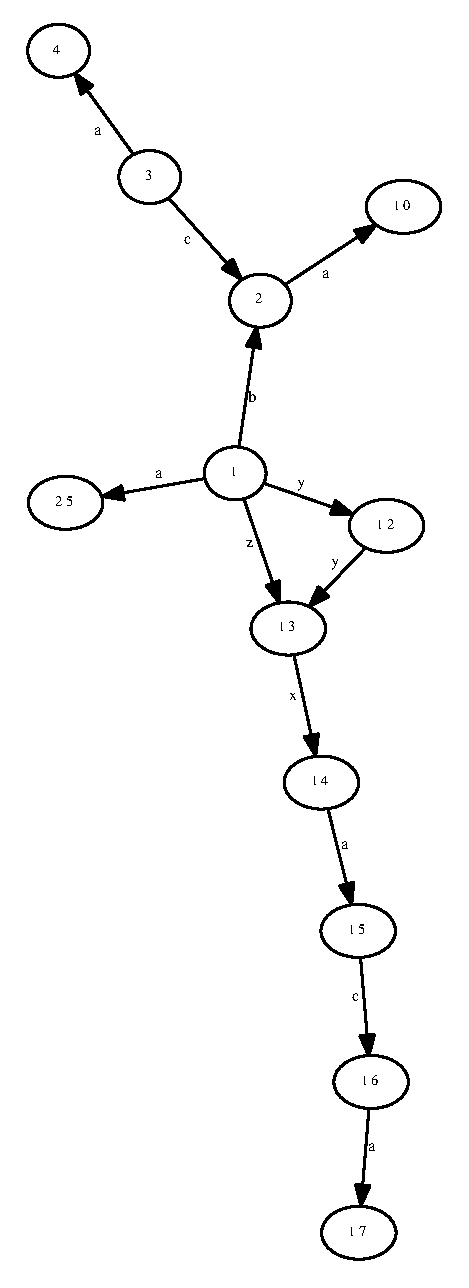
\includegraphics[scale=0.5, bb=0 0 300 600]{python/ex_K_X.eps}
\caption{$X_1$ component $\Theta$}
\label{fig:KX}
\end{center}
\end{figure}

\begin{figure}
\begin{center}
\psfrag{a}{$x_1$}
\psfrag{b}{$x_2$}
\psfrag{c}{$x_3$}
\psfrag{r}{$y_1$}
\psfrag{s}{$y_2$}
\psfrag{t}{$y_3$}
\psfrag{x}{$z_1$}
\psfrag{y}{$z_2$}
\psfrag{z}{$z_3$}
\psfrag{u}{$y_4$}
\psfrag{0}{\hspace{-2pt}\raisebox{-2pt}{\scriptsize $0$}}
\psfrag{1}{\hspace{-2pt}\raisebox{-2pt}{\scriptsize $1$}}
\psfrag{2}{\hspace{-2pt}\raisebox{-2pt}{\scriptsize $2$}}
\psfrag{3}{\hspace{-2pt}\raisebox{-2pt}{\scriptsize $3$}}
\psfrag{4}{\hspace{-2pt}\raisebox{-2pt}{\scriptsize $4$}}
\psfrag{5}{\hspace{-2pt}\raisebox{-2pt}{\scriptsize $5$}}
\psfrag{6}{\hspace{-2pt}\raisebox{-2pt}{\scriptsize $6$}}
\psfrag{7}{\hspace{-2pt}\raisebox{-2pt}{\scriptsize $7$}}
\psfrag{8}{\hspace{-2pt}\raisebox{-2pt}{\scriptsize $8$}}
\psfrag{9}{\hspace{-2pt}\raisebox{-2pt}{\scriptsize $9$}}
\psfrag{10}{\hspace{-2pt}\raisebox{-2pt}{\scriptsize $10$}}
\psfrag{11}{\hspace{-2pt}\raisebox{-2pt}{\scriptsize $11$}}
\psfrag{12}{\hspace{-2pt}\raisebox{-2pt}{\scriptsize $12$}}
\psfrag{13}{\hspace{-2pt}\raisebox{-2pt}{\scriptsize $13$}}
\psfrag{14}{\hspace{-2pt}\raisebox{-2pt}{\scriptsize $14$}}
\psfrag{15}{\hspace{-2pt}\raisebox{-2pt}{\scriptsize $15$}}
\psfrag{16}{\hspace{-2pt}\raisebox{-2pt}{\scriptsize $16$}}
\psfrag{17}{\hspace{-2pt}\raisebox{-2pt}{\scriptsize $17$}}
\psfrag{18}{\hspace{-2pt}\raisebox{-2pt}{\scriptsize $18$}}
\psfrag{19}{\hspace{-2pt}\raisebox{-2pt}{\scriptsize $19$}}
\psfrag{20}{\hspace{-2pt}\raisebox{-2pt}{\scriptsize $20$}}
\psfrag{21}{\hspace{-2pt}\raisebox{-2pt}{\scriptsize $21$}}
\psfrag{22}{\hspace{-2pt}\raisebox{-2pt}{\scriptsize $22$}}
\psfrag{23}{\hspace{-2pt}\raisebox{-2pt}{\scriptsize $23$}}
\psfrag{24}{\hspace{-2pt}\raisebox{-2pt}{\scriptsize $24$}}
\psfrag{25}{\hspace{-2pt}\raisebox{-2pt}{\scriptsize $25$}}
\psfrag{26}{\hspace{-2pt}\raisebox{-2pt}{\scriptsize $26$}}
\psfrag{27}{\hspace{-2pt}\raisebox{-2pt}{\scriptsize $27$}}
\psfrag{28}{\hspace{-2pt}\raisebox{-2pt}{\scriptsize $28$}}
\psfrag{29}{\hspace{-2pt}\raisebox{-2pt}{\scriptsize $29$}}
\begin{subfigure}[b]{.3\columnwidth}
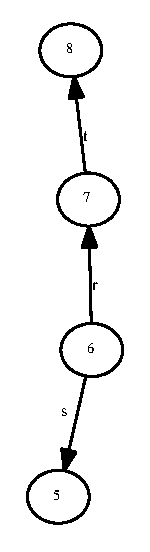
\includegraphics[scale=0.5, bb=0 0  82 280]{python/ex_K_Y1.eps}
\caption{$\Theta^\prime$}
\label{fig:KY1}
\end{subfigure}
\hspace*{2cm}
\begin{subfigure}[b]{.3\columnwidth}
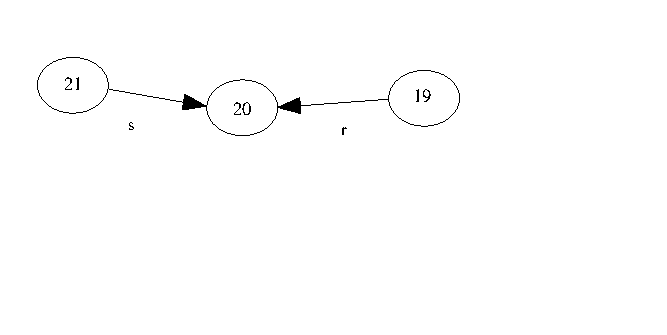
\includegraphics[scale=0.5, bb=0 0 82 210]{python/ex_K_Y2.eps}
\caption{$\Theta^{\prime\prime}$}
\label{fig:KY2}
\end{subfigure}
\end{center}
\caption{$X_2$ components}
\label{fig:KY}
\end{figure}

\begin{figure}
\begin{center}
\psfrag{a}{$x_1$}
\psfrag{b}{$x_2$}
\psfrag{c}{$x_3$}
\psfrag{r}{$y_1$}
\psfrag{s}{$y_2$}
\psfrag{t}{$y_3$}
\psfrag{x}{$z_1$}
\psfrag{y}{$z_2$}
\psfrag{z}{$z_3$}
\psfrag{u}{$y_4$}
\psfrag{0}{\hspace{-2pt}\raisebox{-2pt}{\scriptsize $0$}}
\psfrag{1}{\hspace{-2pt}\raisebox{-2pt}{\scriptsize $1$}}
\psfrag{2}{\hspace{-2pt}\raisebox{-2pt}{\scriptsize $2$}}
\psfrag{3}{\hspace{-2pt}\raisebox{-2pt}{\scriptsize $3$}}
\psfrag{4}{\hspace{-2pt}\raisebox{-2pt}{\scriptsize $4$}}
\psfrag{5}{\hspace{-2pt}\raisebox{-2pt}{\scriptsize $5$}}
\psfrag{6}{\hspace{-2pt}\raisebox{-2pt}{\scriptsize $6$}}
\psfrag{7}{\hspace{-2pt}\raisebox{-2pt}{\scriptsize $7$}}
\psfrag{8}{\hspace{-2pt}\raisebox{-2pt}{\scriptsize $8$}}
\psfrag{9}{\hspace{-2pt}\raisebox{-2pt}{\scriptsize $9$}}
\psfrag{10}{\hspace{-2pt}\raisebox{-2pt}{\scriptsize $10$}}
\psfrag{11}{\hspace{-2pt}\raisebox{-2pt}{\scriptsize $11$}}
\psfrag{12}{\hspace{-2pt}\raisebox{-2pt}{\scriptsize $12$}}
\psfrag{13}{\hspace{-2pt}\raisebox{-2pt}{\scriptsize $13$}}
\psfrag{14}{\hspace{-2pt}\raisebox{-2pt}{\scriptsize $14$}}
\psfrag{15}{\hspace{-2pt}\raisebox{-2pt}{\scriptsize $15$}}
\psfrag{16}{\hspace{-2pt}\raisebox{-2pt}{\scriptsize $16$}}
\psfrag{17}{\hspace{-2pt}\raisebox{-2pt}{\scriptsize $17$}}
\psfrag{18}{\hspace{-2pt}\raisebox{-2pt}{\scriptsize $18$}}
\psfrag{19}{\hspace{-2pt}\raisebox{-2pt}{\scriptsize $19$}}
\psfrag{20}{\hspace{-2pt}\raisebox{-2pt}{\scriptsize $20$}}
\psfrag{21}{\hspace{-2pt}\raisebox{-2pt}{\scriptsize $21$}}
\psfrag{22}{\hspace{-2pt}\raisebox{-2pt}{\scriptsize $22$}}
\psfrag{23}{\hspace{-2pt}\raisebox{-2pt}{\scriptsize $23$}}
\psfrag{24}{\hspace{-2pt}\raisebox{-2pt}{\scriptsize $24$}}
\psfrag{25}{\hspace{-2pt}\raisebox{-2pt}{\scriptsize $25$}}
\psfrag{26}{\hspace{-2pt}\raisebox{-2pt}{\scriptsize $26$}}
\psfrag{27}{\hspace{-2pt}\raisebox{-2pt}{\scriptsize $27$}}
\psfrag{28}{\hspace{-2pt}\raisebox{-2pt}{\scriptsize $28$}}
\psfrag{29}{\hspace{-2pt}\raisebox{-2pt}{\scriptsize $29$}}
\psfrag{30}{\hspace{-2pt}\raisebox{-2pt}{\scriptsize $30$}}
\psfrag{31}{\hspace{-2pt}\raisebox{-2pt}{\scriptsize $31$}}
\psfrag{32}{\hspace{-2pt}\raisebox{-2pt}{\scriptsize $32$}}
\psfrag{33}{\hspace{-2pt}\raisebox{-2pt}{\scriptsize $33$}}
\psfrag{34}{\hspace{-2pt}\raisebox{-2pt}{\scriptsize $34$}}
\psfrag{35}{\hspace{-2pt}\raisebox{-2pt}{\scriptsize $35$}}
\psfrag{36}{\hspace{-2pt}\raisebox{-2pt}{\scriptsize $36$}}
\psfrag{37}{\hspace{-2pt}\raisebox{-2pt}{\scriptsize $37$}}
\psfrag{38}{\hspace{-2pt}\raisebox{-2pt}{\scriptsize $38$}}
\psfrag{39}{\hspace{-2pt}\raisebox{-2pt}{\scriptsize $39$}}
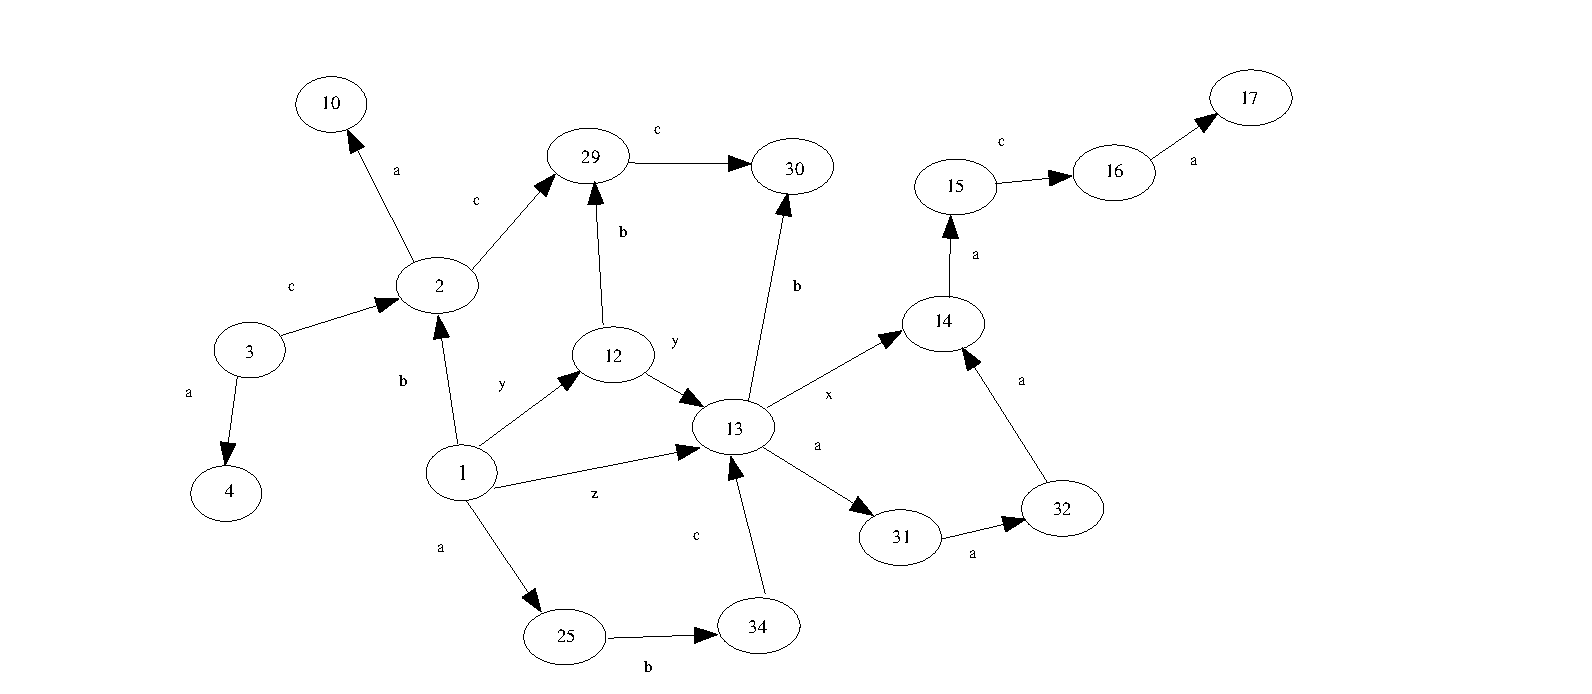
\includegraphics[scale=0.5, bb=0 0 680 480]{python/ex_K_f1.eps}
\caption{$X_1$ component $\Theta_1$}
\label{fig:K_f1}
\end{center}
\end{figure}

\begin{figure}
\begin{center}
\psfrag{1-1}{\hspace{-4pt}\raisebox{-2pt}{\scriptsize $1,1$}}
\psfrag{1-2}{\hspace{-4pt}\raisebox{-2pt}{\scriptsize $1,2$}}
\psfrag{1-3}{\hspace{-4pt}\raisebox{-2pt}{\scriptsize $1,3$}}
\psfrag{1-4}{\hspace{-4pt}\raisebox{-2pt}{\scriptsize $1,4$}}
\psfrag{1-5}{\hspace{-4pt}\raisebox{-2pt}{\scriptsize $1,5$}}
\psfrag{1-6}{\hspace{-4pt}\raisebox{-2pt}{\scriptsize $1,6$}}
\psfrag{1-7}{\hspace{-4pt}\raisebox{-2pt}{\scriptsize $1,7$}}
\psfrag{1-8}{\hspace{-4pt}\raisebox{-2pt}{\scriptsize $1,8$}}
\psfrag{1-9}{\hspace{-4pt}\raisebox{-2pt}{\scriptsize $1,9$}}
\psfrag{2-1}{\hspace{-4pt}\raisebox{-2pt}{\scriptsize $2,1$}}
\psfrag{2-2}{\hspace{-4pt}\raisebox{-2pt}{\scriptsize $2,2$}}
\psfrag{2-3}{\hspace{-4pt}\raisebox{-2pt}{\scriptsize $2,3$}}
\psfrag{2-4}{\hspace{-4pt}\raisebox{-2pt}{\scriptsize $2,4$}}
\psfrag{2-5}{\hspace{-4pt}\raisebox{-2pt}{\scriptsize $2,5$}}
\psfrag{2-6}{\hspace{-4pt}\raisebox{-2pt}{\scriptsize $2,6$}}
\psfrag{2-7}{\hspace{-4pt}\raisebox{-2pt}{\scriptsize $2,7$}}
\psfrag{2-8}{\hspace{-4pt}\raisebox{-2pt}{\scriptsize $2,8$}}
\psfrag{2-9}{\hspace{-4pt}\raisebox{-2pt}{\scriptsize $2,9$}}
\psfrag{3-1}{\hspace{-4pt}\raisebox{-2pt}{\scriptsize $3,1$}}
\psfrag{3-2}{\hspace{-4pt}\raisebox{-2pt}{\scriptsize $3,2$}}
\psfrag{3-3}{\hspace{-4pt}\raisebox{-2pt}{\scriptsize $3,3$}}
\psfrag{3-4}{\hspace{-4pt}\raisebox{-2pt}{\scriptsize $3,4$}}
\psfrag{3-5}{\hspace{-4pt}\raisebox{-2pt}{\scriptsize $3,5$}}
\psfrag{3-6}{\hspace{-4pt}\raisebox{-2pt}{\scriptsize $3,6$}}
\psfrag{3-7}{\hspace{-4pt}\raisebox{-2pt}{\scriptsize $3,7$}}
\psfrag{3-8}{\hspace{-4pt}\raisebox{-2pt}{\scriptsize $3,8$}}
\psfrag{3-9}{\hspace{-4pt}\raisebox{-2pt}{\scriptsize $3,9$}}
\psfrag{4-1}{\hspace{-4pt}\raisebox{-2pt}{\scriptsize $4,1$}}
\psfrag{4-2}{\hspace{-4pt}\raisebox{-2pt}{\scriptsize $4,2$}}
\psfrag{4-3}{\hspace{-4pt}\raisebox{-2pt}{\scriptsize $4,3$}}
\psfrag{4-4}{\hspace{-4pt}\raisebox{-2pt}{\scriptsize $4,4$}}
\psfrag{4-5}{\hspace{-4pt}\raisebox{-2pt}{\scriptsize $4,5$}}
\psfrag{4-6}{\hspace{-4pt}\raisebox{-2pt}{\scriptsize $4,6$}}
\psfrag{4-7}{\hspace{-4pt}\raisebox{-2pt}{\scriptsize $4,7$}}
\psfrag{4-8}{\hspace{-4pt}\raisebox{-2pt}{\scriptsize $4,8$}}
\psfrag{4-9}{\hspace{-4pt}\raisebox{-2pt}{\scriptsize $4,9$}}
\psfrag{5-1}{\hspace{-4pt}\raisebox{-2pt}{\scriptsize $5,1$}}
\psfrag{5-2}{\hspace{-4pt}\raisebox{-2pt}{\scriptsize $5,2$}}
\psfrag{5-3}{\hspace{-4pt}\raisebox{-2pt}{\scriptsize $5,3$}}
\psfrag{5-4}{\hspace{-4pt}\raisebox{-2pt}{\scriptsize $5,4$}}
\psfrag{5-5}{\hspace{-4pt}\raisebox{-2pt}{\scriptsize $5,5$}}
\psfrag{5-6}{\hspace{-4pt}\raisebox{-2pt}{\scriptsize $5,6$}}
\psfrag{5-7}{\hspace{-4pt}\raisebox{-2pt}{\scriptsize $5,7$}}
\psfrag{5-8}{\hspace{-4pt}\raisebox{-2pt}{\scriptsize $5,8$}}
\psfrag{5-9}{\hspace{-4pt}\raisebox{-2pt}{\scriptsize $5,9$}}
\psfrag{6-1}{\hspace{-4pt}\raisebox{-2pt}{\scriptsize $6,1$}}
\psfrag{6-2}{\hspace{-4pt}\raisebox{-2pt}{\scriptsize $6,2$}}
\psfrag{6-3}{\hspace{-4pt}\raisebox{-2pt}{\scriptsize $6,3$}}
\psfrag{6-4}{\hspace{-4pt}\raisebox{-2pt}{\scriptsize $6,4$}}
\psfrag{6-5}{\hspace{-4pt}\raisebox{-2pt}{\scriptsize $6,5$}}
\psfrag{6-6}{\hspace{-4pt}\raisebox{-2pt}{\scriptsize $6,6$}}
\psfrag{6-7}{\hspace{-4pt}\raisebox{-2pt}{\scriptsize $6,7$}}
\psfrag{6-8}{\hspace{-4pt}\raisebox{-2pt}{\scriptsize $6,8$}}
\psfrag{6-9}{\hspace{-4pt}\raisebox{-2pt}{\scriptsize $6,9$}}
\psfrag{7-1}{\hspace{-4pt}\raisebox{-2pt}{\scriptsize $7,1$}}
\psfrag{7-2}{\hspace{-4pt}\raisebox{-2pt}{\scriptsize $7,2$}}
\psfrag{7-3}{\hspace{-4pt}\raisebox{-2pt}{\scriptsize $7,3$}}
\psfrag{7-4}{\hspace{-4pt}\raisebox{-2pt}{\scriptsize $7,4$}}
\psfrag{7-5}{\hspace{-4pt}\raisebox{-2pt}{\scriptsize $7,5$}}
\psfrag{7-6}{\hspace{-4pt}\raisebox{-2pt}{\scriptsize $7,6$}}
\psfrag{7-7}{\hspace{-4pt}\raisebox{-2pt}{\scriptsize $7,7$}}
\psfrag{7-8}{\hspace{-4pt}\raisebox{-2pt}{\scriptsize $7,8$}}
\psfrag{7-9}{\hspace{-4pt}\raisebox{-2pt}{\scriptsize $7,9$}}
\psfrag{8-1}{\hspace{-4pt}\raisebox{-2pt}{\scriptsize $8,1$}}
\psfrag{8-2}{\hspace{-4pt}\raisebox{-2pt}{\scriptsize $8,2$}}
\psfrag{8-3}{\hspace{-4pt}\raisebox{-2pt}{\scriptsize $8,3$}}
\psfrag{8-4}{\hspace{-4pt}\raisebox{-2pt}{\scriptsize $8,4$}}
\psfrag{8-5}{\hspace{-4pt}\raisebox{-2pt}{\scriptsize $8,5$}}
\psfrag{8-6}{\hspace{-4pt}\raisebox{-2pt}{\scriptsize $8,6$}}
\psfrag{8-7}{\hspace{-4pt}\raisebox{-2pt}{\scriptsize $8,7$}}
\psfrag{8-8}{\hspace{-4pt}\raisebox{-2pt}{\scriptsize $8,8$}}
\psfrag{8-9}{\hspace{-4pt}\raisebox{-2pt}{\scriptsize $8,9$}}
\psfrag{9-1}{\hspace{-4pt}\raisebox{-2pt}{\scriptsize $9,1$}}
\psfrag{9-2}{\hspace{-4pt}\raisebox{-2pt}{\scriptsize $9,2$}}
\psfrag{9-3}{\hspace{-4pt}\raisebox{-2pt}{\scriptsize $9,3$}}
\psfrag{9-4}{\hspace{-4pt}\raisebox{-2pt}{\scriptsize $9,4$}}
\psfrag{9-5}{\hspace{-4pt}\raisebox{-2pt}{\scriptsize $9,5$}}
\psfrag{9-6}{\hspace{-4pt}\raisebox{-2pt}{\scriptsize $9,6$}}
\psfrag{9-7}{\hspace{-4pt}\raisebox{-2pt}{\scriptsize $9,7$}}
\psfrag{9-8}{\hspace{-4pt}\raisebox{-2pt}{\scriptsize $9,8$}}
\psfrag{9-9}{\hspace{-4pt}\raisebox{-2pt}{\scriptsize $9,9$}}
\psfrag{10-1}{\hspace{-4pt}\raisebox{-2pt}{\scriptsize $10,1$}}
\psfrag{10-2}{\hspace{-4pt}\raisebox{-2pt}{\scriptsize $10,2$}}
\psfrag{10-3}{\hspace{-4pt}\raisebox{-2pt}{\scriptsize $10,3$}}
\psfrag{10-4}{\hspace{-4pt}\raisebox{-2pt}{\scriptsize $10,4$}}
\psfrag{10-5}{\hspace{-4pt}\raisebox{-2pt}{\scriptsize $10,5$}}
\psfrag{10-6}{\hspace{-4pt}\raisebox{-2pt}{\scriptsize $10,6$}}
\psfrag{10-7}{\hspace{-4pt}\raisebox{-2pt}{\scriptsize $10,7$}}
\psfrag{10-8}{\hspace{-4pt}\raisebox{-2pt}{\scriptsize $10,8$}}
\psfrag{10-9}{\hspace{-4pt}\raisebox{-2pt}{\scriptsize $10,9$}}
\psfrag{11-1}{\hspace{-4pt}\raisebox{-2pt}{\scriptsize $11,1$}}
\psfrag{11-2}{\hspace{-4pt}\raisebox{-2pt}{\scriptsize $11,2$}}
\psfrag{11-3}{\hspace{-4pt}\raisebox{-2pt}{\scriptsize $11,3$}}
\psfrag{11-4}{\hspace{-4pt}\raisebox{-2pt}{\scriptsize $11,4$}}
\psfrag{11-5}{\hspace{-4pt}\raisebox{-2pt}{\scriptsize $11,5$}}
\psfrag{11-6}{\hspace{-4pt}\raisebox{-2pt}{\scriptsize $11,6$}}
\psfrag{11-7}{\hspace{-4pt}\raisebox{-2pt}{\scriptsize $11,7$}}
\psfrag{11-8}{\hspace{-4pt}\raisebox{-2pt}{\scriptsize $11,8$}}
\psfrag{11-9}{\hspace{-4pt}\raisebox{-2pt}{\scriptsize $11,9$}}
\psfrag{12-1}{\hspace{-4pt}\raisebox{-2pt}{\scriptsize $12,1$}}
\psfrag{12-2}{\hspace{-4pt}\raisebox{-2pt}{\scriptsize $12,2$}}
\psfrag{12-3}{\hspace{-4pt}\raisebox{-2pt}{\scriptsize $12,3$}}
\psfrag{12-4}{\hspace{-4pt}\raisebox{-2pt}{\scriptsize $12,4$}}
\psfrag{12-5}{\hspace{-4pt}\raisebox{-2pt}{\scriptsize $12,5$}}
\psfrag{12-6}{\hspace{-4pt}\raisebox{-2pt}{\scriptsize $12,6$}}
\psfrag{12-7}{\hspace{-4pt}\raisebox{-2pt}{\scriptsize $12,7$}}
\psfrag{12-8}{\hspace{-4pt}\raisebox{-2pt}{\scriptsize $12,8$}}
\psfrag{12-9}{\hspace{-4pt}\raisebox{-2pt}{\scriptsize $12,9$}}
\psfrag{13-1}{\hspace{-4pt}\raisebox{-2pt}{\scriptsize $13,1$}}
\psfrag{13-2}{\hspace{-4pt}\raisebox{-2pt}{\scriptsize $13,2$}}
\psfrag{13-3}{\hspace{-4pt}\raisebox{-2pt}{\scriptsize $13,3$}}
\psfrag{13-4}{\hspace{-4pt}\raisebox{-2pt}{\scriptsize $13,4$}}
\psfrag{13-5}{\hspace{-4pt}\raisebox{-2pt}{\scriptsize $13,5$}}
\psfrag{13-6}{\hspace{-4pt}\raisebox{-2pt}{\scriptsize $13,6$}}
\psfrag{13-7}{\hspace{-4pt}\raisebox{-2pt}{\scriptsize $13,7$}}
\psfrag{13-8}{\hspace{-4pt}\raisebox{-2pt}{\scriptsize $13,8$}}
\psfrag{13-9}{\hspace{-4pt}\raisebox{-2pt}{\scriptsize $13,9$}}
\psfrag{14-1}{\hspace{-4pt}\raisebox{-2pt}{\scriptsize $14,1$}}
\psfrag{14-2}{\hspace{-4pt}\raisebox{-2pt}{\scriptsize $14,2$}}
\psfrag{14-3}{\hspace{-4pt}\raisebox{-2pt}{\scriptsize $14,3$}}
\psfrag{14-4}{\hspace{-4pt}\raisebox{-2pt}{\scriptsize $14,4$}}
\psfrag{14-5}{\hspace{-4pt}\raisebox{-2pt}{\scriptsize $14,5$}}
\psfrag{14-6}{\hspace{-4pt}\raisebox{-2pt}{\scriptsize $14,6$}}
\psfrag{14-7}{\hspace{-4pt}\raisebox{-2pt}{\scriptsize $14,7$}}
\psfrag{14-8}{\hspace{-4pt}\raisebox{-2pt}{\scriptsize $14,8$}}
\psfrag{14-9}{\hspace{-4pt}\raisebox{-2pt}{\scriptsize $14,9$}}
\psfrag{15-1}{\hspace{-4pt}\raisebox{-2pt}{\scriptsize $15,1$}}
\psfrag{15-2}{\hspace{-4pt}\raisebox{-2pt}{\scriptsize $15,2$}}
\psfrag{15-3}{\hspace{-4pt}\raisebox{-2pt}{\scriptsize $15,3$}}
\psfrag{15-4}{\hspace{-4pt}\raisebox{-2pt}{\scriptsize $15,4$}}
\psfrag{15-5}{\hspace{-4pt}\raisebox{-2pt}{\scriptsize $15,5$}}
\psfrag{15-6}{\hspace{-4pt}\raisebox{-2pt}{\scriptsize $15,6$}}
\psfrag{15-7}{\hspace{-4pt}\raisebox{-2pt}{\scriptsize $15,7$}}
\psfrag{15-8}{\hspace{-4pt}\raisebox{-2pt}{\scriptsize $15,8$}}
\psfrag{15-9}{\hspace{-4pt}\raisebox{-2pt}{\scriptsize $15,9$}}
\psfrag{16-1}{\hspace{-4pt}\raisebox{-2pt}{\scriptsize $16,1$}}
\psfrag{16-2}{\hspace{-4pt}\raisebox{-2pt}{\scriptsize $16,2$}}
\psfrag{16-3}{\hspace{-4pt}\raisebox{-2pt}{\scriptsize $16,3$}}
\psfrag{16-4}{\hspace{-4pt}\raisebox{-2pt}{\scriptsize $16,4$}}
\psfrag{16-5}{\hspace{-4pt}\raisebox{-2pt}{\scriptsize $16,5$}}
\psfrag{16-6}{\hspace{-4pt}\raisebox{-2pt}{\scriptsize $16,6$}}
\psfrag{16-7}{\hspace{-4pt}\raisebox{-2pt}{\scriptsize $16,7$}}
\psfrag{16-8}{\hspace{-4pt}\raisebox{-2pt}{\scriptsize $16,8$}}
\psfrag{16-9}{\hspace{-4pt}\raisebox{-2pt}{\scriptsize $16,9$}}
\psfrag{17-1}{\hspace{-4pt}\raisebox{-2pt}{\scriptsize $17,1$}}
\psfrag{17-2}{\hspace{-4pt}\raisebox{-2pt}{\scriptsize $17,2$}}
\psfrag{17-3}{\hspace{-4pt}\raisebox{-2pt}{\scriptsize $17,3$}}
\psfrag{17-4}{\hspace{-4pt}\raisebox{-2pt}{\scriptsize $17,4$}}
\psfrag{17-5}{\hspace{-4pt}\raisebox{-2pt}{\scriptsize $17,5$}}
\psfrag{17-6}{\hspace{-4pt}\raisebox{-2pt}{\scriptsize $17,6$}}
\psfrag{17-7}{\hspace{-4pt}\raisebox{-2pt}{\scriptsize $17,7$}}
\psfrag{17-8}{\hspace{-4pt}\raisebox{-2pt}{\scriptsize $17,8$}}
\psfrag{17-9}{\hspace{-4pt}\raisebox{-2pt}{\scriptsize $17,9$}}
\psfrag{18-1}{\hspace{-4pt}\raisebox{-2pt}{\scriptsize $18,1$}}
\psfrag{18-2}{\hspace{-4pt}\raisebox{-2pt}{\scriptsize $18,2$}}
\psfrag{18-3}{\hspace{-4pt}\raisebox{-2pt}{\scriptsize $18,3$}}
\psfrag{18-4}{\hspace{-4pt}\raisebox{-2pt}{\scriptsize $18,4$}}
\psfrag{18-5}{\hspace{-4pt}\raisebox{-2pt}{\scriptsize $18,5$}}
\psfrag{18-6}{\hspace{-4pt}\raisebox{-2pt}{\scriptsize $18,6$}}
\psfrag{18-7}{\hspace{-4pt}\raisebox{-2pt}{\scriptsize $18,7$}}
\psfrag{18-8}{\hspace{-4pt}\raisebox{-2pt}{\scriptsize $18,8$}}
\psfrag{18-9}{\hspace{-4pt}\raisebox{-2pt}{\scriptsize $18,9$}}
\psfrag{19-1}{\hspace{-4pt}\raisebox{-2pt}{\scriptsize $19,1$}}
\psfrag{19-2}{\hspace{-4pt}\raisebox{-2pt}{\scriptsize $19,2$}}
\psfrag{19-3}{\hspace{-4pt}\raisebox{-2pt}{\scriptsize $19,3$}}
\psfrag{19-4}{\hspace{-4pt}\raisebox{-2pt}{\scriptsize $19,4$}}
\psfrag{19-5}{\hspace{-4pt}\raisebox{-2pt}{\scriptsize $19,5$}}
\psfrag{19-6}{\hspace{-4pt}\raisebox{-2pt}{\scriptsize $19,6$}}
\psfrag{19-7}{\hspace{-4pt}\raisebox{-2pt}{\scriptsize $19,7$}}
\psfrag{19-8}{\hspace{-4pt}\raisebox{-2pt}{\scriptsize $19,8$}}
\psfrag{19-9}{\hspace{-4pt}\raisebox{-2pt}{\scriptsize $19,9$}}
\psfrag{20-1}{\hspace{-4pt}\raisebox{-2pt}{\scriptsize $20,1$}}
\psfrag{20-2}{\hspace{-4pt}\raisebox{-2pt}{\scriptsize $20,2$}}
\psfrag{20-3}{\hspace{-4pt}\raisebox{-2pt}{\scriptsize $20,3$}}
\psfrag{20-4}{\hspace{-4pt}\raisebox{-2pt}{\scriptsize $20,4$}}
\psfrag{20-5}{\hspace{-4pt}\raisebox{-2pt}{\scriptsize $20,5$}}
\psfrag{20-6}{\hspace{-4pt}\raisebox{-2pt}{\scriptsize $20,6$}}
\psfrag{20-7}{\hspace{-4pt}\raisebox{-2pt}{\scriptsize $20,7$}}
\psfrag{20-8}{\hspace{-4pt}\raisebox{-2pt}{\scriptsize $20,8$}}
\psfrag{20-9}{\hspace{-4pt}\raisebox{-2pt}{\scriptsize $20,9$}}
\psfrag{21-1}{\hspace{-4pt}\raisebox{-2pt}{\scriptsize $21,1$}}
\psfrag{21-2}{\hspace{-4pt}\raisebox{-2pt}{\scriptsize $21,2$}}
\psfrag{21-3}{\hspace{-4pt}\raisebox{-2pt}{\scriptsize $21,3$}}
\psfrag{21-4}{\hspace{-4pt}\raisebox{-2pt}{\scriptsize $21,4$}}
\psfrag{21-5}{\hspace{-4pt}\raisebox{-2pt}{\scriptsize $21,5$}}
\psfrag{21-6}{\hspace{-4pt}\raisebox{-2pt}{\scriptsize $21,6$}}
\psfrag{21-7}{\hspace{-4pt}\raisebox{-2pt}{\scriptsize $21,7$}}
\psfrag{21-8}{\hspace{-4pt}\raisebox{-2pt}{\scriptsize $21,8$}}
\psfrag{21-9}{\hspace{-4pt}\raisebox{-2pt}{\scriptsize $21,9$}}
\psfrag{22-1}{\hspace{-4pt}\raisebox{-2pt}{\scriptsize $22,1$}}
\psfrag{22-2}{\hspace{-4pt}\raisebox{-2pt}{\scriptsize $22,2$}}
\psfrag{22-3}{\hspace{-4pt}\raisebox{-2pt}{\scriptsize $22,3$}}
\psfrag{22-4}{\hspace{-4pt}\raisebox{-2pt}{\small
 $22,4$}}
\psfrag{22-5}{\hspace{-4pt}\raisebox{-2pt}{\scriptsize $22,5$}}
\psfrag{22-6}{\hspace{-4pt}\raisebox{-2pt}{\scriptsize $22,6$}}
\psfrag{22-7}{\hspace{-4pt}\raisebox{-2pt}{\scriptsize $22,7$}}
\psfrag{22-8}{\hspace{-4pt}\raisebox{-2pt}{\scriptsize $22,8$}}
\psfrag{22-9}{\hspace{-4pt}\raisebox{-2pt}{\scriptsize $22,9$}}
\psfrag{23-1}{\hspace{-4pt}\raisebox{-2pt}{\scriptsize $23,1$}}
\psfrag{23-2}{\hspace{-4pt}\raisebox{-2pt}{\scriptsize $23,2$}}
\psfrag{23-3}{\hspace{-4pt}\raisebox{-2pt}{\scriptsize $23,3$}}
\psfrag{23-4}{\hspace{-4pt}\raisebox{-2pt}{\scriptsize $23,4$}}
\psfrag{23-5}{\hspace{-4pt}\raisebox{-2pt}{\scriptsize $23,5$}}
\psfrag{23-6}{\hspace{-4pt}\raisebox{-2pt}{\small
 $23,6$}}
\psfrag{23-7}{\hspace{-4pt}\raisebox{-2pt}{\scriptsize $23,7$}}
\psfrag{23-8}{\hspace{-4pt}\raisebox{-2pt}{\scriptsize $23,8$}}
\psfrag{23-9}{\hspace{-4pt}\raisebox{-2pt}{\scriptsize $23,9$}}
\psfrag{24-1}{\hspace{-4pt}\raisebox{-2pt}{\scriptsize $24,1$}}
\psfrag{24-2}{\hspace{-4pt}\raisebox{-2pt}{\scriptsize $24,2$}}
\psfrag{24-3}{\hspace{-4pt}\raisebox{-2pt}{\scriptsize $24,3$}}
\psfrag{24-4}{\hspace{-4pt}\raisebox{-2pt}{\scriptsize $24,4$}}
\psfrag{24-5}{\hspace{-4pt}\raisebox{-2pt}{\scriptsize $24,5$}}
\psfrag{24-6}{\hspace{-4pt}\raisebox{-2pt}{\scriptsize $24,6$}}
\psfrag{24-7}{\hspace{-4pt}\raisebox{-2pt}{\scriptsize $24,7$}}
\psfrag{24-8}{\hspace{-4pt}\raisebox{-2pt}{\scriptsize $24,8$}}
\psfrag{24-9}{\hspace{-4pt}\raisebox{-2pt}{\scriptsize $24,9$}}
\psfrag{25-1}{\hspace{-4pt}\raisebox{-2pt}{\scriptsize $25,1$}}
\psfrag{25-2}{\hspace{-4pt}\raisebox{-2pt}{\scriptsize $25,2$}}
\psfrag{25-3}{\hspace{-4pt}\raisebox{-2pt}{\scriptsize $25,3$}}
\psfrag{25-4}{\hspace{-4pt}\raisebox{-2pt}{\scriptsize $25,4$}}
\psfrag{25-5}{\hspace{-4pt}\raisebox{-2pt}{\scriptsize $25,5$}}
\psfrag{25-6}{\hspace{-4pt}\raisebox{-2pt}{\scriptsize $25,6$}}
\psfrag{25-7}{\hspace{-4pt}\raisebox{-2pt}{\scriptsize $25,7$}}
\psfrag{25-8}{\hspace{-4pt}\raisebox{-2pt}{\scriptsize $25,8$}}
\psfrag{25-9}{\hspace{-4pt}\raisebox{-2pt}{\scriptsize $25,9$}}
\psfrag{26-1}{\hspace{-4pt}\raisebox{-2pt}{\scriptsize $26,1$}}
\psfrag{26-2}{\hspace{-4pt}\raisebox{-2pt}{\scriptsize $26,2$}}
\psfrag{26-3}{\hspace{-4pt}\raisebox{-2pt}{\scriptsize $26,3$}}
\psfrag{26-4}{\hspace{-4pt}\raisebox{-2pt}{\scriptsize $26,4$}}
\psfrag{26-5}{\hspace{-4pt}\raisebox{-2pt}{\scriptsize $26,5$}}
\psfrag{26-6}{\hspace{-4pt}\raisebox{-2pt}{\scriptsize $26,6$}}
\psfrag{26-7}{\hspace{-4pt}\raisebox{-2pt}{\scriptsize $26,7$}}
\psfrag{26-8}{\hspace{-4pt}\raisebox{-2pt}{\scriptsize $26,8$}}
\psfrag{26-9}{\hspace{-4pt}\raisebox{-2pt}{\scriptsize $26,9$}}
\psfrag{27-1}{\hspace{-4pt}\raisebox{-2pt}{\scriptsize $27,1$}}
\psfrag{27-2}{\hspace{-4pt}\raisebox{-2pt}{\scriptsize $27,2$}}
\psfrag{27-3}{\hspace{-4pt}\raisebox{-2pt}{\scriptsize $27,3$}}
\psfrag{27-4}{\hspace{-4pt}\raisebox{-2pt}{\scriptsize $27,4$}}
\psfrag{27-5}{\hspace{-4pt}\raisebox{-2pt}{\scriptsize $27,5$}}
\psfrag{27-6}{\hspace{-4pt}\raisebox{-2pt}{\scriptsize $27,6$}}
\psfrag{27-7}{\hspace{-4pt}\raisebox{-2pt}{\scriptsize $27,7$}}
\psfrag{27-8}{\hspace{-4pt}\raisebox{-2pt}{\scriptsize $27,8$}}
\psfrag{27-9}{\hspace{-4pt}\raisebox{-2pt}{\scriptsize $27,9$}}
\psfrag{28-1}{\hspace{-4pt}\raisebox{-2pt}{\scriptsize $28,1$}}
\psfrag{28-2}{\hspace{-4pt}\raisebox{-2pt}{\scriptsize $28,2$}}
\psfrag{28-3}{\hspace{-4pt}\raisebox{-2pt}{\scriptsize $28,3$}}
\psfrag{28-4}{\hspace{-4pt}\raisebox{-2pt}{\scriptsize $28,4$}}
\psfrag{28-5}{\hspace{-4pt}\raisebox{-2pt}{\scriptsize $28,5$}}
\psfrag{28-6}{\hspace{-4pt}\raisebox{-2pt}{\scriptsize $28,6$}}
\psfrag{28-7}{\hspace{-4pt}\raisebox{-2pt}{\scriptsize $28,7$}}
\psfrag{28-8}{\hspace{-4pt}\raisebox{-2pt}{\scriptsize $28,8$}}
\psfrag{28-9}{\hspace{-4pt}\raisebox{-2pt}{\scriptsize $28,9$}}
\psfrag{29-1}{\hspace{-4pt}\raisebox{-2pt}{\scriptsize $29,1$}}
\psfrag{29-2}{\hspace{-4pt}\raisebox{-2pt}{\scriptsize $29,2$}}
\psfrag{29-3}{\hspace{-4pt}\raisebox{-2pt}{\scriptsize $29,3$}}
\psfrag{29-4}{\hspace{-4pt}\raisebox{-2pt}{\scriptsize $29,4$}}
\psfrag{29-5}{\hspace{-4pt}\raisebox{-2pt}{\scriptsize $29,5$}}
\psfrag{29-6}{\hspace{-4pt}\raisebox{-2pt}{\scriptsize $29,6$}}
\psfrag{29-7}{\hspace{-4pt}\raisebox{-2pt}{\scriptsize $29,7$}}
\psfrag{29-8}{\hspace{-4pt}\raisebox{-2pt}{\scriptsize $29,8$}}
\psfrag{29-9}{\hspace{-4pt}\raisebox{-2pt}{\scriptsize $29,9$}}
\psfrag{30-1}{\hspace{-4pt}\raisebox{-2pt}{\scriptsize $30,1$}}
\psfrag{30-2}{\hspace{-4pt}\raisebox{-2pt}{\scriptsize $30,2$}}
\psfrag{30-3}{\hspace{-4pt}\raisebox{-2pt}{\scriptsize $30,3$}}
\psfrag{30-4}{\hspace{-4pt}\raisebox{-2pt}{\scriptsize $30,4$}}
\psfrag{30-5}{\hspace{-4pt}\raisebox{-2pt}{\scriptsize $30,5$}}
\psfrag{30-6}{\hspace{-4pt}\raisebox{-2pt}{\scriptsize $30,6$}}
\psfrag{30-7}{\hspace{-4pt}\raisebox{-2pt}{\scriptsize $30,7$}}
\psfrag{30-8}{\hspace{-4pt}\raisebox{-2pt}{\scriptsize $30,8$}}
\psfrag{30-9}{\hspace{-4pt}\raisebox{-2pt}{\scriptsize $30,9$}}
\psfrag{31-1}{\hspace{-4pt}\raisebox{-2pt}{\scriptsize $31,1$}}
\psfrag{31-2}{\hspace{-4pt}\raisebox{-2pt}{\scriptsize $31,2$}}
\psfrag{31-3}{\hspace{-4pt}\raisebox{-2pt}{\scriptsize $31,3$}}
\psfrag{31-4}{\hspace{-4pt}\raisebox{-2pt}{\scriptsize $31,4$}}
\psfrag{31-5}{\hspace{-4pt}\raisebox{-2pt}{\scriptsize $31,5$}}
\psfrag{31-6}{\hspace{-4pt}\raisebox{-2pt}{\scriptsize $31,6$}}
\psfrag{31-7}{\hspace{-4pt}\raisebox{-2pt}{\scriptsize $31,7$}}
\psfrag{31-8}{\hspace{-4pt}\raisebox{-2pt}{\scriptsize $31,8$}}
\psfrag{31-9}{\hspace{-4pt}\raisebox{-2pt}{\scriptsize $31,9$}}
\psfrag{32-1}{\hspace{-4pt}\raisebox{-2pt}{\scriptsize $32,1$}}
\psfrag{32-2}{\hspace{-4pt}\raisebox{-2pt}{\scriptsize $32,2$}}
\psfrag{32-3}{\hspace{-4pt}\raisebox{-2pt}{\scriptsize $32,3$}}
\psfrag{32-4}{\hspace{-4pt}\raisebox{-2pt}{\scriptsize $32,4$}}
\psfrag{32-5}{\hspace{-4pt}\raisebox{-2pt}{\scriptsize $32,5$}}
\psfrag{32-6}{\hspace{-4pt}\raisebox{-2pt}{\scriptsize $32,6$}}
\psfrag{32-7}{\hspace{-4pt}\raisebox{-2pt}{\scriptsize $32,7$}}
\psfrag{32-8}{\hspace{-4pt}\raisebox{-2pt}{\scriptsize $32,8$}}
\psfrag{32-9}{\hspace{-4pt}\raisebox{-2pt}{\scriptsize $32,9$}}
\psfrag{33-1}{\hspace{-4pt}\raisebox{-2pt}{\scriptsize $33,1$}}
\psfrag{33-2}{\hspace{-4pt}\raisebox{-2pt}{\scriptsize $33,2$}}
\psfrag{33-3}{\hspace{-4pt}\raisebox{-2pt}{\scriptsize $33,3$}}
\psfrag{33-4}{\hspace{-4pt}\raisebox{-2pt}{\scriptsize $33,4$}}
\psfrag{33-5}{\hspace{-4pt}\raisebox{-2pt}{\scriptsize $33,5$}}
\psfrag{33-6}{\hspace{-4pt}\raisebox{-2pt}{\scriptsize $33,6$}}
\psfrag{33-7}{\hspace{-4pt}\raisebox{-2pt}{\scriptsize $33,7$}}
\psfrag{33-8}{\hspace{-4pt}\raisebox{-2pt}{\scriptsize $33,8$}}
\psfrag{33-9}{\hspace{-4pt}\raisebox{-2pt}{\scriptsize $33,9$}}
\psfrag{34-1}{\hspace{-4pt}\raisebox{-2pt}{\scriptsize $34,1$}}
\psfrag{34-2}{\hspace{-4pt}\raisebox{-2pt}{\scriptsize $34,2$}}
\psfrag{34-3}{\hspace{-4pt}\raisebox{-2pt}{\scriptsize $34,3$}}
\psfrag{34-4}{\hspace{-4pt}\raisebox{-2pt}{\scriptsize $34,4$}}
\psfrag{34-5}{\hspace{-4pt}\raisebox{-2pt}{\scriptsize $34,5$}}
\psfrag{34-6}{\hspace{-4pt}\raisebox{-2pt}{\scriptsize $34,6$}}
\psfrag{34-7}{\hspace{-4pt}\raisebox{-2pt}{\scriptsize $34,7$}}
\psfrag{34-8}{\hspace{-4pt}\raisebox{-2pt}{\scriptsize $34,8$}}
\psfrag{34-9}{\hspace{-4pt}\raisebox{-2pt}{\scriptsize $34,9$}}
\psfrag{35-1}{\hspace{-4pt}\raisebox{-2pt}{\scriptsize $35,1$}}
\psfrag{35-2}{\hspace{-4pt}\raisebox{-2pt}{\scriptsize $35,2$}}
\psfrag{35-3}{\hspace{-4pt}\raisebox{-2pt}{\scriptsize $35,3$}}
\psfrag{35-4}{\hspace{-4pt}\raisebox{-2pt}{\scriptsize $35,4$}}
\psfrag{35-5}{\hspace{-4pt}\raisebox{-2pt}{\scriptsize $35,5$}}
\psfrag{35-6}{\hspace{-4pt}\raisebox{-2pt}{\scriptsize $35,6$}}
\psfrag{35-7}{\hspace{-4pt}\raisebox{-2pt}{\scriptsize $35,7$}}
\psfrag{35-8}{\hspace{-4pt}\raisebox{-2pt}{\scriptsize $35,8$}}
\psfrag{35-9}{\hspace{-4pt}\raisebox{-2pt}{\scriptsize $35,9$}}
\psfrag{36-1}{\hspace{-4pt}\raisebox{-2pt}{\scriptsize $36,1$}}
\psfrag{36-2}{\hspace{-4pt}\raisebox{-2pt}{\scriptsize $36,2$}}
\psfrag{36-3}{\hspace{-4pt}\raisebox{-2pt}{\scriptsize $36,3$}}
\psfrag{36-4}{\hspace{-4pt}\raisebox{-2pt}{\scriptsize $36,4$}}
\psfrag{36-5}{\hspace{-4pt}\raisebox{-2pt}{\scriptsize $36,5$}}
\psfrag{36-6}{\hspace{-4pt}\raisebox{-2pt}{\scriptsize $36,6$}}
\psfrag{36-7}{\hspace{-4pt}\raisebox{-2pt}{\scriptsize $36,7$}}
\psfrag{36-8}{\hspace{-4pt}\raisebox{-2pt}{\scriptsize $36,8$}}
\psfrag{36-9}{\hspace{-4pt}\raisebox{-2pt}{\scriptsize $36,9$}}
\psfrag{37-1}{\hspace{-4pt}\raisebox{-2pt}{\scriptsize $37,1$}}
\psfrag{37-2}{\hspace{-4pt}\raisebox{-2pt}{\scriptsize $37,2$}}
\psfrag{37-3}{\hspace{-4pt}\raisebox{-2pt}{\scriptsize $37,3$}}
\psfrag{37-4}{\hspace{-4pt}\raisebox{-2pt}{\scriptsize $37,4$}}
\psfrag{37-5}{\hspace{-4pt}\raisebox{-2pt}{\scriptsize $37,5$}}
\psfrag{37-6}{\hspace{-4pt}\raisebox{-2pt}{\scriptsize $37,6$}}
\psfrag{37-7}{\hspace{-4pt}\raisebox{-2pt}{\scriptsize $37,7$}}
\psfrag{37-8}{\hspace{-4pt}\raisebox{-2pt}{\scriptsize $37,8$}}
\psfrag{37-9}{\hspace{-4pt}\raisebox{-2pt}{\scriptsize $37,9$}}
\psfrag{38-1}{\hspace{-4pt}\raisebox{-2pt}{\scriptsize $38,1$}}
\psfrag{38-2}{\hspace{-4pt}\raisebox{-2pt}{\scriptsize $38,2$}}
\psfrag{38-3}{\hspace{-4pt}\raisebox{-2pt}{\scriptsize $38,3$}}
\psfrag{38-4}{\hspace{-4pt}\raisebox{-2pt}{\scriptsize $38,4$}}
\psfrag{38-5}{\hspace{-4pt}\raisebox{-2pt}{\scriptsize $38,5$}}
\psfrag{38-6}{\hspace{-4pt}\raisebox{-2pt}{\scriptsize $38,6$}}
\psfrag{38-7}{\hspace{-4pt}\raisebox{-2pt}{\scriptsize $38,7$}}
\psfrag{38-8}{\hspace{-4pt}\raisebox{-2pt}{\scriptsize $38,8$}}
\psfrag{38-9}{\hspace{-4pt}\raisebox{-2pt}{\scriptsize $38,9$}}
\psfrag{39-1}{\hspace{-4pt}\raisebox{-2pt}{\scriptsize $39,1$}}
\psfrag{39-2}{\hspace{-4pt}\raisebox{-2pt}{\scriptsize $39,2$}}
\psfrag{39-3}{\hspace{-4pt}\raisebox{-2pt}{\scriptsize $39,3$}}
\psfrag{39-4}{\hspace{-4pt}\raisebox{-2pt}{\scriptsize $39,4$}}
\psfrag{39-5}{\hspace{-4pt}\raisebox{-2pt}{\scriptsize $39,5$}}
\psfrag{39-6}{\hspace{-4pt}\raisebox{-2pt}{\scriptsize $39,6$}}
\psfrag{39-7}{\hspace{-4pt}\raisebox{-2pt}{\scriptsize $39,7$}}
\psfrag{39-8}{\hspace{-4pt}\raisebox{-2pt}{\scriptsize $39,8$}}
\psfrag{39-9}{\hspace{-4pt}\raisebox{-2pt}{\scriptsize $39,9$}}
\psfrag{40-1}{\hspace{-4pt}\raisebox{-2pt}{\scriptsize $40,1$}}
\psfrag{40-2}{\hspace{-4pt}\raisebox{-2pt}{\scriptsize $40,2$}}
\psfrag{40-3}{\hspace{-4pt}\raisebox{-2pt}{\scriptsize $40,3$}}
\psfrag{40-4}{\hspace{-4pt}\raisebox{-2pt}{\scriptsize $40,4$}}
\psfrag{40-5}{\hspace{-4pt}\raisebox{-2pt}{\scriptsize $40,5$}}
\psfrag{40-6}{\hspace{-4pt}\raisebox{-2pt}{\scriptsize $40,6$}}
\psfrag{40-7}{\hspace{-4pt}\raisebox{-2pt}{\scriptsize $40,7$}}
\psfrag{40-8}{\hspace{-4pt}\raisebox{-2pt}{\scriptsize $40,8$}}
\psfrag{40-9}{\hspace{-4pt}\raisebox{-2pt}{\scriptsize $40,9$}}
\psfrag{41-1}{\hspace{-4pt}\raisebox{-2pt}{\scriptsize $41,1$}}
\psfrag{41-2}{\hspace{-4pt}\raisebox{-2pt}{\scriptsize $41,2$}}
\psfrag{41-3}{\hspace{-4pt}\raisebox{-2pt}{\scriptsize $41,3$}}
\psfrag{41-4}{\hspace{-4pt}\raisebox{-2pt}{\scriptsize $41,4$}}
\psfrag{41-5}{\hspace{-4pt}\raisebox{-2pt}{\scriptsize $41,5$}}
\psfrag{41-6}{\hspace{-4pt}\raisebox{-2pt}{\scriptsize $41,6$}}
\psfrag{41-7}{\hspace{-4pt}\raisebox{-2pt}{\scriptsize $41,7$}}
\psfrag{41-8}{\hspace{-4pt}\raisebox{-2pt}{\scriptsize $41,8$}}
\psfrag{41-9}{\hspace{-4pt}\raisebox{-2pt}{\scriptsize $41,9$}}
\psfrag{42-1}{\hspace{-4pt}\raisebox{-2pt}{\scriptsize $42,1$}}
\psfrag{42-2}{\hspace{-4pt}\raisebox{-2pt}{\scriptsize $42,2$}}
\psfrag{42-3}{\hspace{-4pt}\raisebox{-2pt}{\scriptsize $42,3$}}
\psfrag{42-4}{\hspace{-4pt}\raisebox{-2pt}{\scriptsize $42,4$}}
\psfrag{42-5}{\hspace{-4pt}\raisebox{-2pt}{\scriptsize $42,5$}}
\psfrag{42-6}{\hspace{-4pt}\raisebox{-2pt}{\scriptsize $42,6$}}
\psfrag{42-7}{\hspace{-4pt}\raisebox{-2pt}{\scriptsize $42,7$}}
\psfrag{42-8}{\hspace{-4pt}\raisebox{-2pt}{\scriptsize $42,8$}}
\psfrag{42-9}{\hspace{-4pt}\raisebox{-2pt}{\scriptsize $42,9$}}
\psfrag{43-1}{\hspace{-4pt}\raisebox{-2pt}{\scriptsize $43,1$}}
\psfrag{43-2}{\hspace{-4pt}\raisebox{-2pt}{\scriptsize $43,2$}}
\psfrag{43-3}{\hspace{-4pt}\raisebox{-2pt}{\scriptsize $43,3$}}
\psfrag{43-4}{\hspace{-4pt}\raisebox{-2pt}{\scriptsize $43,4$}}
\psfrag{43-5}{\hspace{-4pt}\raisebox{-2pt}{\scriptsize $43,5$}}
\psfrag{43-6}{\hspace{-4pt}\raisebox{-2pt}{\scriptsize $43,6$}}
\psfrag{43-7}{\hspace{-4pt}\raisebox{-2pt}{\scriptsize $43,7$}}
\psfrag{43-8}{\hspace{-4pt}\raisebox{-2pt}{\scriptsize $43,8$}}
\psfrag{43-9}{\hspace{-4pt}\raisebox{-2pt}{\scriptsize $43,9$}}
\psfrag{44-1}{\hspace{-4pt}\raisebox{-2pt}{\scriptsize $44,1$}}
\psfrag{44-2}{\hspace{-4pt}\raisebox{-2pt}{\scriptsize $44,2$}}
\psfrag{44-3}{\hspace{-4pt}\raisebox{-2pt}{\scriptsize $44,3$}}
\psfrag{44-4}{\hspace{-4pt}\raisebox{-2pt}{\scriptsize $44,4$}}
\psfrag{44-5}{\hspace{-4pt}\raisebox{-2pt}{\scriptsize $44,5$}}
\psfrag{44-6}{\hspace{-4pt}\raisebox{-2pt}{\scriptsize $44,6$}}
\psfrag{44-7}{\hspace{-4pt}\raisebox{-2pt}{\scriptsize $44,7$}}
\psfrag{44-8}{\hspace{-4pt}\raisebox{-2pt}{\scriptsize $44,8$}}
\psfrag{44-9}{\hspace{-4pt}\raisebox{-2pt}{\scriptsize $44,9$}}
\psfrag{45-1}{\hspace{-4pt}\raisebox{-2pt}{\scriptsize $45,1$}}
\psfrag{45-2}{\hspace{-4pt}\raisebox{-2pt}{\scriptsize $45,2$}}
\psfrag{45-3}{\hspace{-4pt}\raisebox{-2pt}{\scriptsize $45,3$}}
\psfrag{45-4}{\hspace{-4pt}\raisebox{-2pt}{\scriptsize $45,4$}}
\psfrag{45-5}{\hspace{-4pt}\raisebox{-2pt}{\scriptsize $45,5$}}
\psfrag{45-6}{\hspace{-4pt}\raisebox{-2pt}{\scriptsize $45,6$}}
\psfrag{45-7}{\hspace{-4pt}\raisebox{-2pt}{\scriptsize $45,7$}}
\psfrag{45-8}{\hspace{-4pt}\raisebox{-2pt}{\scriptsize $45,8$}}
\psfrag{45-9}{\hspace{-4pt}\raisebox{-2pt}{\scriptsize $45,9$}}
\psfrag{46-1}{\hspace{-4pt}\raisebox{-2pt}{\scriptsize $46,1$}}
\psfrag{46-2}{\hspace{-4pt}\raisebox{-2pt}{\scriptsize $46,2$}}
\psfrag{46-3}{\hspace{-4pt}\raisebox{-2pt}{\scriptsize $46,3$}}
\psfrag{46-4}{\hspace{-4pt}\raisebox{-2pt}{\scriptsize $46,4$}}
\psfrag{46-5}{\hspace{-4pt}\raisebox{-2pt}{\scriptsize $46,5$}}
\psfrag{46-6}{\hspace{-4pt}\raisebox{-2pt}{\scriptsize $46,6$}}
\psfrag{46-7}{\hspace{-4pt}\raisebox{-2pt}{\scriptsize $46,7$}}
\psfrag{46-8}{\hspace{-4pt}\raisebox{-2pt}{\scriptsize $46,8$}}
\psfrag{46-9}{\hspace{-4pt}\raisebox{-2pt}{\scriptsize $46,9$}}
\psfrag{47-1}{\hspace{-4pt}\raisebox{-2pt}{\scriptsize $47,1$}}
\psfrag{47-2}{\hspace{-4pt}\raisebox{-2pt}{\scriptsize $47,2$}}
\psfrag{47-3}{\hspace{-4pt}\raisebox{-2pt}{\scriptsize $47,3$}}
\psfrag{47-4}{\hspace{-4pt}\raisebox{-2pt}{\scriptsize $47,4$}}
\psfrag{47-5}{\hspace{-4pt}\raisebox{-2pt}{\scriptsize $47,5$}}
\psfrag{47-6}{\hspace{-4pt}\raisebox{-2pt}{\scriptsize $47,6$}}
\psfrag{47-7}{\hspace{-4pt}\raisebox{-2pt}{\scriptsize $47,7$}}
\psfrag{47-8}{\hspace{-4pt}\raisebox{-2pt}{\scriptsize $47,8$}}
\psfrag{47-9}{\hspace{-4pt}\raisebox{-2pt}{\scriptsize $47,9$}}
\psfrag{48-1}{\hspace{-4pt}\raisebox{-2pt}{\scriptsize $48,1$}}
\psfrag{48-2}{\hspace{-4pt}\raisebox{-2pt}{\scriptsize $48,2$}}
\psfrag{48-3}{\hspace{-4pt}\raisebox{-2pt}{\scriptsize $48,3$}}
\psfrag{48-4}{\hspace{-4pt}\raisebox{-2pt}{\scriptsize $48,4$}}
\psfrag{48-5}{\hspace{-4pt}\raisebox{-2pt}{\scriptsize $48,5$}}
\psfrag{48-6}{\hspace{-4pt}\raisebox{-2pt}{\scriptsize $48,6$}}
\psfrag{48-7}{\hspace{-4pt}\raisebox{-2pt}{\scriptsize $48,7$}}
\psfrag{48-8}{\hspace{-4pt}\raisebox{-2pt}{\scriptsize $48,8$}}
\psfrag{48-9}{\hspace{-4pt}\raisebox{-2pt}{\scriptsize $48,9$}}
\psfrag{49-1}{\hspace{-4pt}\raisebox{-2pt}{\scriptsize $49,1$}}
\psfrag{49-2}{\hspace{-4pt}\raisebox{-2pt}{\scriptsize $49,2$}}
\psfrag{49-3}{\hspace{-4pt}\raisebox{-2pt}{\scriptsize $49,3$}}
\psfrag{49-4}{\hspace{-4pt}\raisebox{-2pt}{\scriptsize $49,4$}}
\psfrag{49-5}{\hspace{-4pt}\raisebox{-2pt}{\scriptsize $49,5$}}
\psfrag{49-6}{\hspace{-4pt}\raisebox{-2pt}{\scriptsize $49,6$}}
\psfrag{49-7}{\hspace{-4pt}\raisebox{-2pt}{\scriptsize $49,7$}}
\psfrag{49-8}{\hspace{-4pt}\raisebox{-2pt}{\scriptsize $49,8$}}
\psfrag{49-9}{\hspace{-4pt}\raisebox{-2pt}{\scriptsize $49,9$}}
\psfrag{a}{$x_1$}
\psfrag{b}{$x_2$}
\psfrag{c}{$x_3$}
\psfrag{r}{$y_1$}
\psfrag{s}{$y_2$}
\psfrag{t}{$y_3$}
\psfrag{x}{$z_1$}
\psfrag{y}{$z_2$}
\psfrag{z}{$z_3$}
\psfrag{u}{$y_4$}
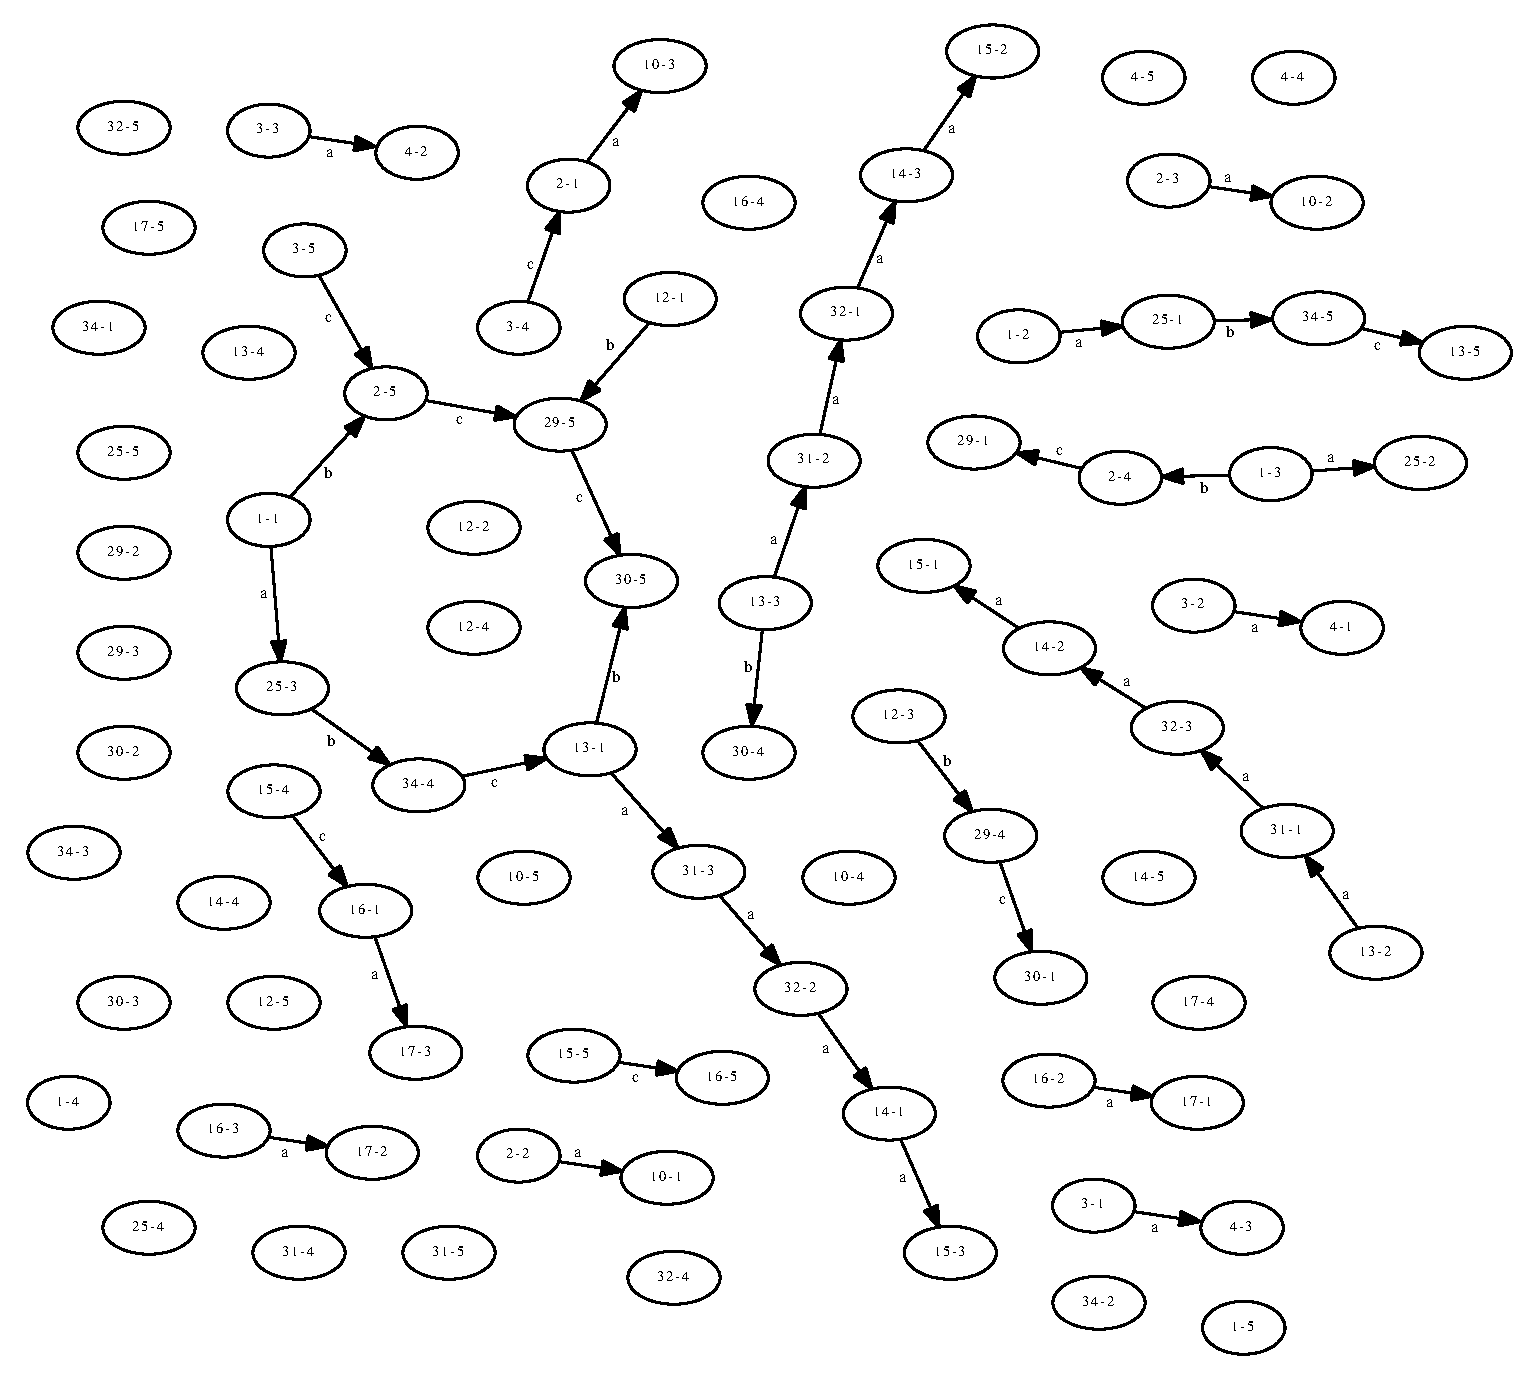
\includegraphics[scale=0.5, bb=0 0 790 700]{python/ex_K_f1-x-g.eps}
\caption{$\cP_1=\Theta_1\times \G_{A_1}$}
\label{fig:K_f1-x-g}
\end{center}
\end{figure}


\begin{figure}
\begin{center}
\psfrag{a}{$x_1$}
\psfrag{b}{$x_2$}
\psfrag{c}{$x_3$}
\psfrag{r}{$y_1$}
\psfrag{s}{$y_2$}
\psfrag{t}{$y_3$}
\psfrag{x}{$z_1$}
\psfrag{y}{$z_2$}
\psfrag{z}{$z_3$}
\psfrag{u}{$y_4$}
%\psfrag{1}{$1$}
\psfrag{0}{\hspace{-2pt}\raisebox{-2pt}{\scriptsize $0$}}
\psfrag{1}{\hspace{-2pt}\raisebox{-2pt}{\scriptsize $1$}}
\psfrag{2}{\hspace{-2pt}\raisebox{-2pt}{\scriptsize $2$}}
\psfrag{3}{\hspace{-2pt}\raisebox{-2pt}{\scriptsize $3$}}
\psfrag{4}{\hspace{-2pt}\raisebox{-2pt}{\scriptsize $4$}}
\psfrag{5}{\hspace{-2pt}\raisebox{-2pt}{\scriptsize $5$}}
\psfrag{6}{\hspace{-2pt}\raisebox{-2pt}{\scriptsize $6$}}
\psfrag{7}{\hspace{-2pt}\raisebox{-2pt}{\scriptsize $7$}}
\psfrag{8}{\hspace{-2pt}\raisebox{-2pt}{\scriptsize $8$}}
\psfrag{9}{\hspace{-2pt}\raisebox{-2pt}{\scriptsize $9$}}
\psfrag{10}{\hspace{-2pt}\raisebox{-2pt}{\scriptsize $10$}}
\psfrag{11}{\hspace{-2pt}\raisebox{-2pt}{\scriptsize $11$}}
\psfrag{12}{\hspace{-2pt}\raisebox{-2pt}{\scriptsize $12$}}
\psfrag{13}{\hspace{-2pt}\raisebox{-2pt}{\scriptsize $13$}}
\psfrag{14}{\hspace{-2pt}\raisebox{-2pt}{\scriptsize $14$}}
\psfrag{15}{\hspace{-2pt}\raisebox{-2pt}{\scriptsize $15$}}
\psfrag{16}{\hspace{-2pt}\raisebox{-2pt}{\scriptsize $16$}}
\psfrag{17}{\hspace{-2pt}\raisebox{-2pt}{\scriptsize $17$}}
\psfrag{18}{\hspace{-2pt}\raisebox{-2pt}{\scriptsize $18$}}
\psfrag{19}{\hspace{-2pt}\raisebox{-2pt}{\scriptsize $19$}}
\psfrag{20}{\hspace{-2pt}\raisebox{-2pt}{\scriptsize $20$}}
\psfrag{21}{\hspace{-2pt}\raisebox{-2pt}{\scriptsize $21$}}
\psfrag{22}{\hspace{-2pt}\raisebox{-2pt}{\scriptsize $22$}}
\psfrag{23}{\hspace{-2pt}\raisebox{-2pt}{\scriptsize $23$}}
\psfrag{24}{\hspace{-2pt}\raisebox{-2pt}{\scriptsize $24$}}
\psfrag{25}{\hspace{-2pt}\raisebox{-2pt}{\scriptsize $25$}}
\psfrag{26}{\hspace{-2pt}\raisebox{-2pt}{\scriptsize $26$}}
\psfrag{27}{\hspace{-2pt}\raisebox{-2pt}{\scriptsize $27$}}
\psfrag{28}{\hspace{-2pt}\raisebox{-2pt}{\scriptsize $28$}}
\psfrag{29}{\hspace{-2pt}\raisebox{-2pt}{\scriptsize $29$}}
\psfrag{30}{\hspace{-2pt}\raisebox{-2pt}{\scriptsize $30$}}
\psfrag{31}{\hspace{-2pt}\raisebox{-2pt}{\scriptsize $31$}}
\psfrag{32}{\hspace{-2pt}\raisebox{-2pt}{\scriptsize $32$}}
\psfrag{33}{\hspace{-2pt}\raisebox{-2pt}{\scriptsize $33$}}
\psfrag{34}{\hspace{-2pt}\raisebox{-2pt}{\scriptsize $34$}}
\psfrag{35}{\hspace{-2pt}\raisebox{-2pt}{\scriptsize $35$}}
\psfrag{36}{\hspace{-2pt}\raisebox{-2pt}{\scriptsize $36$}}
\psfrag{37}{\hspace{-2pt}\raisebox{-2pt}{\scriptsize $37$}}
\psfrag{38}{\hspace{-2pt}\raisebox{-2pt}{\scriptsize $38$}}
\psfrag{39}{\hspace{-2pt}\raisebox{-2pt}{\scriptsize $39$}}
%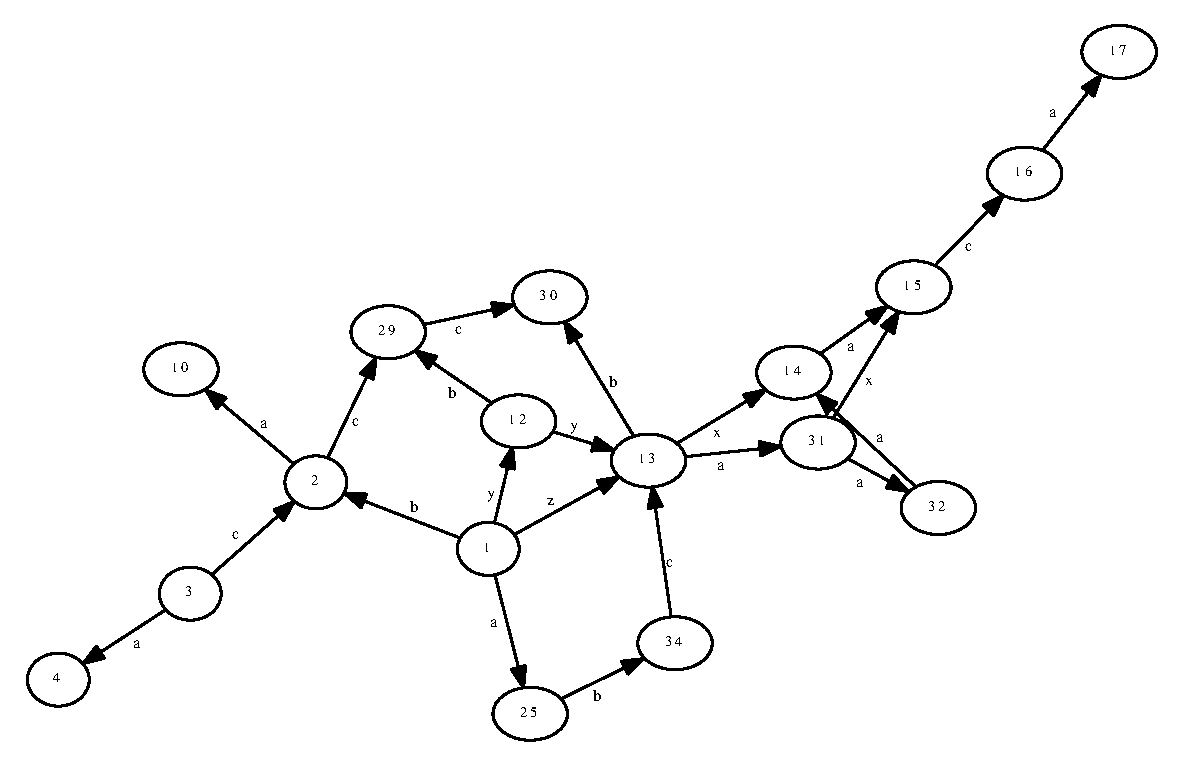
\includegraphics[scale=0.5, bb=50 200 580 580]{python/ex_K_f2.eps}
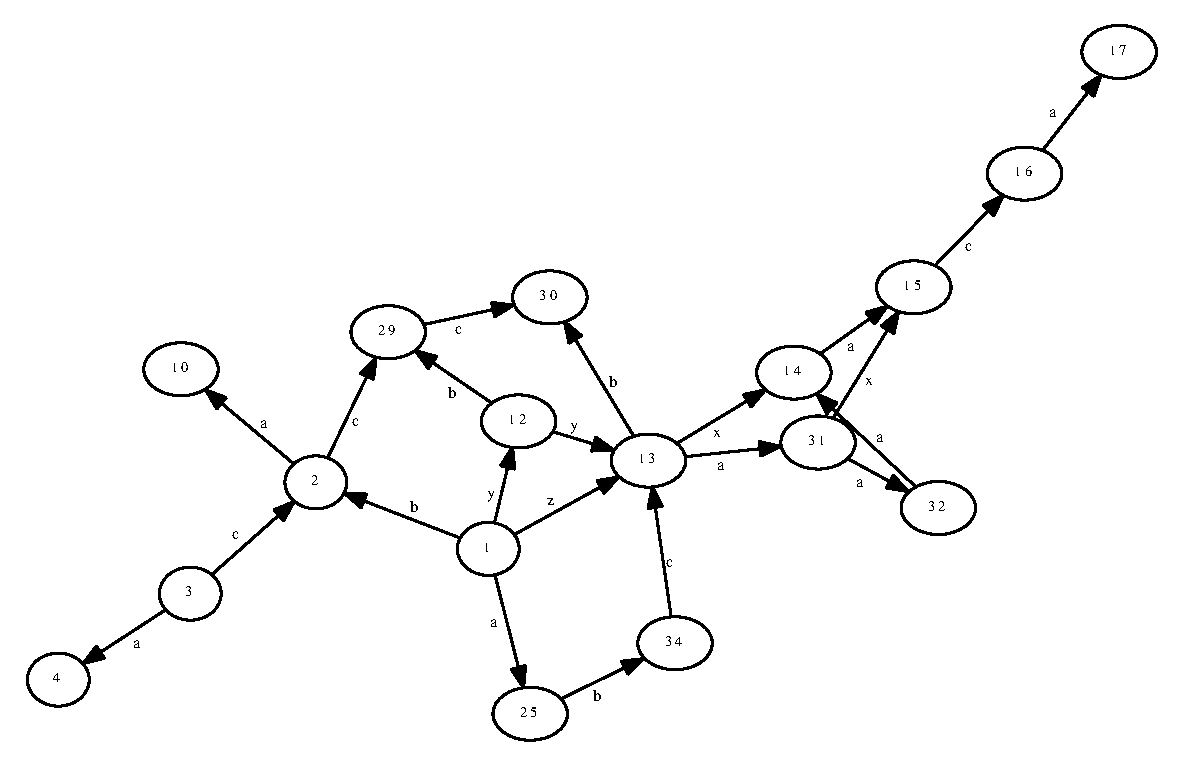
\includegraphics[scale=0.5, bb=0 0 630 410]{python/ex_K_f2.eps}
\caption{$X_1$ component $\Theta_2$}
\label{fig:K_f2}
\end{center}
\end{figure}


\begin{figure}
\begin{center}
\psfrag{a}{$x_1$}
\psfrag{b}{$x_2$}
\psfrag{c}{$x_3$}
\psfrag{r}{$y_1$}
\psfrag{s}{$y_2$}
\psfrag{t}{$y_3$}
\psfrag{x}{$z_1$}
\psfrag{y}{$z_2$}
\psfrag{z}{$z_3$}
\psfrag{u}{$y_4$}
\psfrag{0}{\hspace{-2pt}\raisebox{-2pt}{\scriptsize $0$}}
\psfrag{1}{\hspace{-2pt}\raisebox{-2pt}{\scriptsize $1$}}
\psfrag{2}{\hspace{-2pt}\raisebox{-2pt}{\scriptsize $2$}}
\psfrag{3}{\hspace{-2pt}\raisebox{-2pt}{\scriptsize $3$}}
\psfrag{4}{\hspace{-2pt}\raisebox{-2pt}{\scriptsize $4$}}
\psfrag{5}{\hspace{-2pt}\raisebox{-2pt}{\scriptsize $5$}}
\psfrag{6}{\hspace{-2pt}\raisebox{-2pt}{\scriptsize $6$}}
\psfrag{7}{\hspace{-2pt}\raisebox{-2pt}{\scriptsize $7$}}
\psfrag{8}{\hspace{-2pt}\raisebox{-2pt}{\scriptsize $8$}}
\psfrag{9}{\hspace{-2pt}\raisebox{-2pt}{\scriptsize $9$}}
\psfrag{10}{\hspace{-2pt}\raisebox{-2pt}{\scriptsize $10$}}
\psfrag{11}{\hspace{-2pt}\raisebox{-2pt}{\scriptsize $11$}}
\psfrag{12}{\hspace{-2pt}\raisebox{-2pt}{\scriptsize $12$}}
\psfrag{13}{\hspace{-2pt}\raisebox{-2pt}{\scriptsize $13$}}
\psfrag{14}{\hspace{-2pt}\raisebox{-2pt}{\scriptsize $14$}}
\psfrag{15}{\hspace{-2pt}\raisebox{-2pt}{\scriptsize $15$}}
\psfrag{16}{\hspace{-2pt}\raisebox{-2pt}{\scriptsize $16$}}
\psfrag{17}{\hspace{-2pt}\raisebox{-2pt}{\scriptsize $17$}}
\psfrag{18}{\hspace{-2pt}\raisebox{-2pt}{\scriptsize $18$}}
\psfrag{19}{\hspace{-2pt}\raisebox{-2pt}{\scriptsize $19$}}
\psfrag{20}{\hspace{-2pt}\raisebox{-2pt}{\scriptsize $20$}}
\psfrag{21}{\hspace{-2pt}\raisebox{-2pt}{\scriptsize $21$}}
\psfrag{22}{\hspace{-2pt}\raisebox{-2pt}{\scriptsize $22$}}
\psfrag{23}{\hspace{-2pt}\raisebox{-2pt}{\scriptsize $23$}}
\psfrag{24}{\hspace{-2pt}\raisebox{-2pt}{\scriptsize $24$}}
\psfrag{25}{\hspace{-2pt}\raisebox{-2pt}{\scriptsize $25$}}
\psfrag{26}{\hspace{-2pt}\raisebox{-2pt}{\scriptsize $26$}}
\psfrag{27}{\hspace{-2pt}\raisebox{-2pt}{\scriptsize $27$}}
\psfrag{28}{\hspace{-2pt}\raisebox{-2pt}{\scriptsize $28$}}
\psfrag{29}{\hspace{-2pt}\raisebox{-2pt}{\scriptsize $29$}}
\psfrag{30}{\hspace{-2pt}\raisebox{-2pt}{\scriptsize $30$}}
\psfrag{31}{\hspace{-2pt}\raisebox{-2pt}{\scriptsize $31$}}
\psfrag{32}{\hspace{-2pt}\raisebox{-2pt}{\scriptsize $32$}}
\psfrag{33}{\hspace{-2pt}\raisebox{-2pt}{\scriptsize $33$}}
\psfrag{34}{\hspace{-2pt}\raisebox{-2pt}{\scriptsize $34$}}
\psfrag{35}{\hspace{-2pt}\raisebox{-2pt}{\scriptsize $35$}}
\psfrag{36}{\hspace{-2pt}\raisebox{-2pt}{\scriptsize $36$}}
\psfrag{37}{\hspace{-2pt}\raisebox{-2pt}{\scriptsize $37$}}
\psfrag{38}{\hspace{-2pt}\raisebox{-2pt}{\scriptsize $38$}}
\psfrag{39}{\hspace{-2pt}\raisebox{-2pt}{\scriptsize $39$}}
\psfrag{40}{\hspace{-2pt}\raisebox{-2pt}{\scriptsize $40$}}
\psfrag{41}{\hspace{-2pt}\raisebox{-2pt}{\scriptsize $41$}}
\psfrag{42}{\hspace{-2pt}\raisebox{-2pt}{\scriptsize $42$}}
\psfrag{43}{\hspace{-2pt}\raisebox{-2pt}{\scriptsize $43$}}
\psfrag{44}{\hspace{-2pt}\raisebox{-2pt}{\scriptsize $44$}}
\psfrag{45}{\hspace{-2pt}\raisebox{-2pt}{\scriptsize $45$}}
\psfrag{46}{\hspace{-2pt}\raisebox{-2pt}{\scriptsize $46$}}
\psfrag{47}{\hspace{-2pt}\raisebox{-2pt}{\scriptsize $47$}}
\psfrag{48}{\hspace{-2pt}\raisebox{-2pt}{\scriptsize $48$}}
\psfrag{49}{\hspace{-2pt}\raisebox{-2pt}{\scriptsize $49$}}
%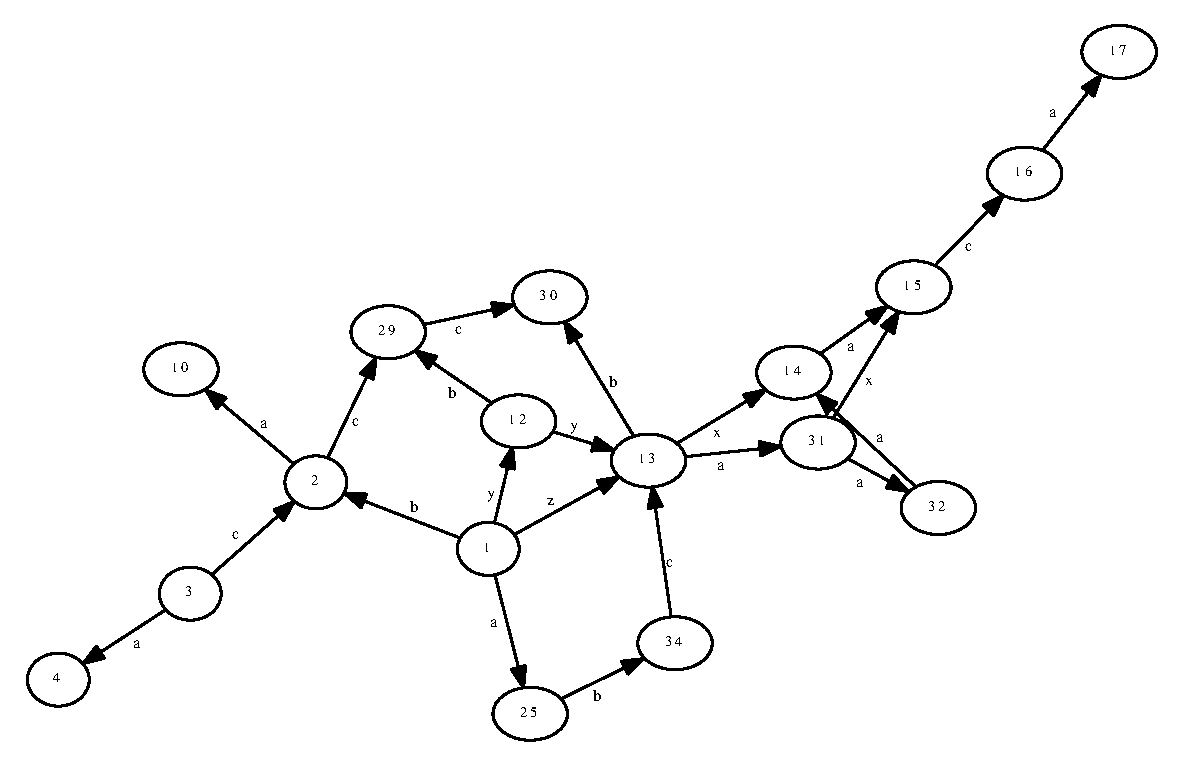
\includegraphics[scale=0.5, bb=50 200 580 580]{python/ex_K_f2.eps}
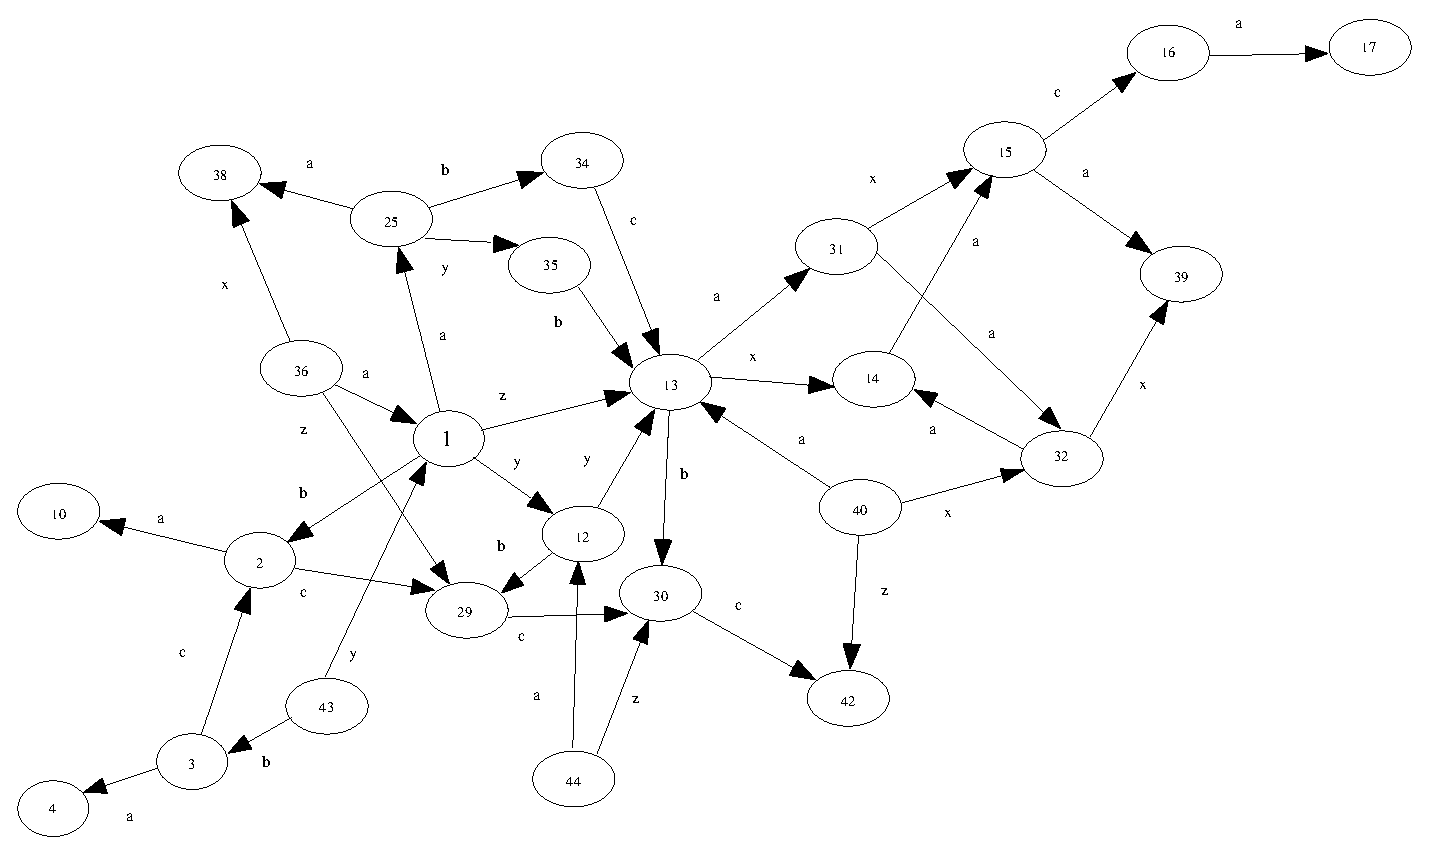
\includegraphics[scale=0.55, bb=0 0 710 420]{python/ex_K_f4.eps}
\caption{$X_1$ component $\Theta_4$}
\label{fig:K_f4}
\end{center}
\end{figure}


\begin{figure}
\begin{center}
\psfrag{1-1}{\hspace{-4pt}\raisebox{-2pt}{\scriptsize $1,1$}}
\psfrag{1-2}{\hspace{-4pt}\raisebox{-2pt}{\scriptsize $1,2$}}
\psfrag{1-3}{\hspace{-4pt}\raisebox{-2pt}{\scriptsize $1,3$}}
\psfrag{1-4}{\hspace{-4pt}\raisebox{-2pt}{\scriptsize $1,4$}}
\psfrag{1-5}{\hspace{-4pt}\raisebox{-2pt}{\scriptsize $1,5$}}
\psfrag{1-6}{\hspace{-4pt}\raisebox{-2pt}{\scriptsize $1,6$}}
\psfrag{1-7}{\hspace{-4pt}\raisebox{-2pt}{\scriptsize $1,7$}}
\psfrag{1-8}{\hspace{-4pt}\raisebox{-2pt}{\scriptsize $1,8$}}
\psfrag{1-9}{\hspace{-4pt}\raisebox{-2pt}{\scriptsize $1,9$}}
\psfrag{2-1}{\hspace{-4pt}\raisebox{-2pt}{\scriptsize $2,1$}}
\psfrag{2-2}{\hspace{-4pt}\raisebox{-2pt}{\scriptsize $2,2$}}
\psfrag{2-3}{\hspace{-4pt}\raisebox{-2pt}{\scriptsize $2,3$}}
\psfrag{2-4}{\hspace{-4pt}\raisebox{-2pt}{\scriptsize $2,4$}}
\psfrag{2-5}{\hspace{-4pt}\raisebox{-2pt}{\scriptsize $2,5$}}
\psfrag{2-6}{\hspace{-4pt}\raisebox{-2pt}{\scriptsize $2,6$}}
\psfrag{2-7}{\hspace{-4pt}\raisebox{-2pt}{\scriptsize $2,7$}}
\psfrag{2-8}{\hspace{-4pt}\raisebox{-2pt}{\scriptsize $2,8$}}
\psfrag{2-9}{\hspace{-4pt}\raisebox{-2pt}{\scriptsize $2,9$}}
\psfrag{3-1}{\hspace{-4pt}\raisebox{-2pt}{\scriptsize $3,1$}}
\psfrag{3-2}{\hspace{-4pt}\raisebox{-2pt}{\scriptsize $3,2$}}
\psfrag{3-3}{\hspace{-4pt}\raisebox{-2pt}{\scriptsize $3,3$}}
\psfrag{3-4}{\hspace{-4pt}\raisebox{-2pt}{\scriptsize $3,4$}}
\psfrag{3-5}{\hspace{-4pt}\raisebox{-2pt}{\scriptsize $3,5$}}
\psfrag{3-6}{\hspace{-4pt}\raisebox{-2pt}{\scriptsize $3,6$}}
\psfrag{3-7}{\hspace{-4pt}\raisebox{-2pt}{\scriptsize $3,7$}}
\psfrag{3-8}{\hspace{-4pt}\raisebox{-2pt}{\scriptsize $3,8$}}
\psfrag{3-9}{\hspace{-4pt}\raisebox{-2pt}{\scriptsize $3,9$}}
\psfrag{4-1}{\hspace{-4pt}\raisebox{-2pt}{\scriptsize $4,1$}}
\psfrag{4-2}{\hspace{-4pt}\raisebox{-2pt}{\scriptsize $4,2$}}
\psfrag{4-3}{\hspace{-4pt}\raisebox{-2pt}{\scriptsize $4,3$}}
\psfrag{4-4}{\hspace{-4pt}\raisebox{-2pt}{\scriptsize $4,4$}}
\psfrag{4-5}{\hspace{-4pt}\raisebox{-2pt}{\scriptsize $4,5$}}
\psfrag{4-6}{\hspace{-4pt}\raisebox{-2pt}{\scriptsize $4,6$}}
\psfrag{4-7}{\hspace{-4pt}\raisebox{-2pt}{\scriptsize $4,7$}}
\psfrag{4-8}{\hspace{-4pt}\raisebox{-2pt}{\scriptsize $4,8$}}
\psfrag{4-9}{\hspace{-4pt}\raisebox{-2pt}{\scriptsize $4,9$}}
\psfrag{5-1}{\hspace{-4pt}\raisebox{-2pt}{\scriptsize $5,1$}}
\psfrag{5-2}{\hspace{-4pt}\raisebox{-2pt}{\scriptsize $5,2$}}
\psfrag{5-3}{\hspace{-4pt}\raisebox{-2pt}{\scriptsize $5,3$}}
\psfrag{5-4}{\hspace{-4pt}\raisebox{-2pt}{\scriptsize $5,4$}}
\psfrag{5-5}{\hspace{-4pt}\raisebox{-2pt}{\scriptsize $5,5$}}
\psfrag{5-6}{\hspace{-4pt}\raisebox{-2pt}{\scriptsize $5,6$}}
\psfrag{5-7}{\hspace{-4pt}\raisebox{-2pt}{\scriptsize $5,7$}}
\psfrag{5-8}{\hspace{-4pt}\raisebox{-2pt}{\scriptsize $5,8$}}
\psfrag{5-9}{\hspace{-4pt}\raisebox{-2pt}{\scriptsize $5,9$}}
\psfrag{6-1}{\hspace{-4pt}\raisebox{-2pt}{\scriptsize $6,1$}}
\psfrag{6-2}{\hspace{-4pt}\raisebox{-2pt}{\scriptsize $6,2$}}
\psfrag{6-3}{\hspace{-4pt}\raisebox{-2pt}{\scriptsize $6,3$}}
\psfrag{6-4}{\hspace{-4pt}\raisebox{-2pt}{\scriptsize $6,4$}}
\psfrag{6-5}{\hspace{-4pt}\raisebox{-2pt}{\scriptsize $6,5$}}
\psfrag{6-6}{\hspace{-4pt}\raisebox{-2pt}{\scriptsize $6,6$}}
\psfrag{6-7}{\hspace{-4pt}\raisebox{-2pt}{\scriptsize $6,7$}}
\psfrag{6-8}{\hspace{-4pt}\raisebox{-2pt}{\scriptsize $6,8$}}
\psfrag{6-9}{\hspace{-4pt}\raisebox{-2pt}{\scriptsize $6,9$}}
\psfrag{7-1}{\hspace{-4pt}\raisebox{-2pt}{\scriptsize $7,1$}}
\psfrag{7-2}{\hspace{-4pt}\raisebox{-2pt}{\scriptsize $7,2$}}
\psfrag{7-3}{\hspace{-4pt}\raisebox{-2pt}{\scriptsize $7,3$}}
\psfrag{7-4}{\hspace{-4pt}\raisebox{-2pt}{\scriptsize $7,4$}}
\psfrag{7-5}{\hspace{-4pt}\raisebox{-2pt}{\scriptsize $7,5$}}
\psfrag{7-6}{\hspace{-4pt}\raisebox{-2pt}{\scriptsize $7,6$}}
\psfrag{7-7}{\hspace{-4pt}\raisebox{-2pt}{\scriptsize $7,7$}}
\psfrag{7-8}{\hspace{-4pt}\raisebox{-2pt}{\scriptsize $7,8$}}
\psfrag{7-9}{\hspace{-4pt}\raisebox{-2pt}{\scriptsize $7,9$}}
\psfrag{8-1}{\hspace{-4pt}\raisebox{-2pt}{\scriptsize $8,1$}}
\psfrag{8-2}{\hspace{-4pt}\raisebox{-2pt}{\scriptsize $8,2$}}
\psfrag{8-3}{\hspace{-4pt}\raisebox{-2pt}{\scriptsize $8,3$}}
\psfrag{8-4}{\hspace{-4pt}\raisebox{-2pt}{\scriptsize $8,4$}}
\psfrag{8-5}{\hspace{-4pt}\raisebox{-2pt}{\scriptsize $8,5$}}
\psfrag{8-6}{\hspace{-4pt}\raisebox{-2pt}{\scriptsize $8,6$}}
\psfrag{8-7}{\hspace{-4pt}\raisebox{-2pt}{\scriptsize $8,7$}}
\psfrag{8-8}{\hspace{-4pt}\raisebox{-2pt}{\scriptsize $8,8$}}
\psfrag{8-9}{\hspace{-4pt}\raisebox{-2pt}{\scriptsize $8,9$}}
\psfrag{9-1}{\hspace{-4pt}\raisebox{-2pt}{\scriptsize $9,1$}}
\psfrag{9-2}{\hspace{-4pt}\raisebox{-2pt}{\scriptsize $9,2$}}
\psfrag{9-3}{\hspace{-4pt}\raisebox{-2pt}{\scriptsize $9,3$}}
\psfrag{9-4}{\hspace{-4pt}\raisebox{-2pt}{\scriptsize $9,4$}}
\psfrag{9-5}{\hspace{-4pt}\raisebox{-2pt}{\scriptsize $9,5$}}
\psfrag{9-6}{\hspace{-4pt}\raisebox{-2pt}{\scriptsize $9,6$}}
\psfrag{9-7}{\hspace{-4pt}\raisebox{-2pt}{\scriptsize $9,7$}}
\psfrag{9-8}{\hspace{-4pt}\raisebox{-2pt}{\scriptsize $9,8$}}
\psfrag{9-9}{\hspace{-4pt}\raisebox{-2pt}{\scriptsize $9,9$}}
\psfrag{10-1}{\hspace{-4pt}\raisebox{-2pt}{\scriptsize $10,1$}}
\psfrag{10-2}{\hspace{-4pt}\raisebox{-2pt}{\scriptsize $10,2$}}
\psfrag{10-3}{\hspace{-4pt}\raisebox{-2pt}{\scriptsize $10,3$}}
\psfrag{10-4}{\hspace{-4pt}\raisebox{-2pt}{\scriptsize $10,4$}}
\psfrag{10-5}{\hspace{-4pt}\raisebox{-2pt}{\scriptsize $10,5$}}
\psfrag{10-6}{\hspace{-4pt}\raisebox{-2pt}{\scriptsize $10,6$}}
\psfrag{10-7}{\hspace{-4pt}\raisebox{-2pt}{\scriptsize $10,7$}}
\psfrag{10-8}{\hspace{-4pt}\raisebox{-2pt}{\scriptsize $10,8$}}
\psfrag{10-9}{\hspace{-4pt}\raisebox{-2pt}{\scriptsize $10,9$}}
\psfrag{11-1}{\hspace{-4pt}\raisebox{-2pt}{\scriptsize $11,1$}}
\psfrag{11-2}{\hspace{-4pt}\raisebox{-2pt}{\scriptsize $11,2$}}
\psfrag{11-3}{\hspace{-4pt}\raisebox{-2pt}{\scriptsize $11,3$}}
\psfrag{11-4}{\hspace{-4pt}\raisebox{-2pt}{\scriptsize $11,4$}}
\psfrag{11-5}{\hspace{-4pt}\raisebox{-2pt}{\scriptsize $11,5$}}
\psfrag{11-6}{\hspace{-4pt}\raisebox{-2pt}{\scriptsize $11,6$}}
\psfrag{11-7}{\hspace{-4pt}\raisebox{-2pt}{\scriptsize $11,7$}}
\psfrag{11-8}{\hspace{-4pt}\raisebox{-2pt}{\scriptsize $11,8$}}
\psfrag{11-9}{\hspace{-4pt}\raisebox{-2pt}{\scriptsize $11,9$}}
\psfrag{12-1}{\hspace{-4pt}\raisebox{-2pt}{\scriptsize $12,1$}}
\psfrag{12-2}{\hspace{-4pt}\raisebox{-2pt}{\scriptsize $12,2$}}
\psfrag{12-3}{\hspace{-4pt}\raisebox{-2pt}{\scriptsize $12,3$}}
\psfrag{12-4}{\hspace{-4pt}\raisebox{-2pt}{\scriptsize $12,4$}}
\psfrag{12-5}{\hspace{-4pt}\raisebox{-2pt}{\scriptsize $12,5$}}
\psfrag{12-6}{\hspace{-4pt}\raisebox{-2pt}{\scriptsize $12,6$}}
\psfrag{12-7}{\hspace{-4pt}\raisebox{-2pt}{\scriptsize $12,7$}}
\psfrag{12-8}{\hspace{-4pt}\raisebox{-2pt}{\scriptsize $12,8$}}
\psfrag{12-9}{\hspace{-4pt}\raisebox{-2pt}{\scriptsize $12,9$}}
\psfrag{13-1}{\hspace{-4pt}\raisebox{-2pt}{\scriptsize $13,1$}}
\psfrag{13-2}{\hspace{-4pt}\raisebox{-2pt}{\scriptsize $13,2$}}
\psfrag{13-3}{\hspace{-4pt}\raisebox{-2pt}{\scriptsize $13,3$}}
\psfrag{13-4}{\hspace{-4pt}\raisebox{-2pt}{\scriptsize $13,4$}}
\psfrag{13-5}{\hspace{-4pt}\raisebox{-2pt}{\scriptsize $13,5$}}
\psfrag{13-6}{\hspace{-4pt}\raisebox{-2pt}{\scriptsize $13,6$}}
\psfrag{13-7}{\hspace{-4pt}\raisebox{-2pt}{\scriptsize $13,7$}}
\psfrag{13-8}{\hspace{-4pt}\raisebox{-2pt}{\scriptsize $13,8$}}
\psfrag{13-9}{\hspace{-4pt}\raisebox{-2pt}{\scriptsize $13,9$}}
\psfrag{14-1}{\hspace{-4pt}\raisebox{-2pt}{\scriptsize $14,1$}}
\psfrag{14-2}{\hspace{-4pt}\raisebox{-2pt}{\scriptsize $14,2$}}
\psfrag{14-3}{\hspace{-4pt}\raisebox{-2pt}{\scriptsize $14,3$}}
\psfrag{14-4}{\hspace{-4pt}\raisebox{-2pt}{\scriptsize $14,4$}}
\psfrag{14-5}{\hspace{-4pt}\raisebox{-2pt}{\scriptsize $14,5$}}
\psfrag{14-6}{\hspace{-4pt}\raisebox{-2pt}{\scriptsize $14,6$}}
\psfrag{14-7}{\hspace{-4pt}\raisebox{-2pt}{\scriptsize $14,7$}}
\psfrag{14-8}{\hspace{-4pt}\raisebox{-2pt}{\scriptsize $14,8$}}
\psfrag{14-9}{\hspace{-4pt}\raisebox{-2pt}{\scriptsize $14,9$}}
\psfrag{15-1}{\hspace{-4pt}\raisebox{-2pt}{\scriptsize $15,1$}}
\psfrag{15-2}{\hspace{-4pt}\raisebox{-2pt}{\scriptsize $15,2$}}
\psfrag{15-3}{\hspace{-4pt}\raisebox{-2pt}{\scriptsize $15,3$}}
\psfrag{15-4}{\hspace{-4pt}\raisebox{-2pt}{\scriptsize $15,4$}}
\psfrag{15-5}{\hspace{-4pt}\raisebox{-2pt}{\scriptsize $15,5$}}
\psfrag{15-6}{\hspace{-4pt}\raisebox{-2pt}{\scriptsize $15,6$}}
\psfrag{15-7}{\hspace{-4pt}\raisebox{-2pt}{\scriptsize $15,7$}}
\psfrag{15-8}{\hspace{-4pt}\raisebox{-2pt}{\scriptsize $15,8$}}
\psfrag{15-9}{\hspace{-4pt}\raisebox{-2pt}{\scriptsize $15,9$}}
\psfrag{16-1}{\hspace{-4pt}\raisebox{-2pt}{\scriptsize $16,1$}}
\psfrag{16-2}{\hspace{-4pt}\raisebox{-2pt}{\scriptsize $16,2$}}
\psfrag{16-3}{\hspace{-4pt}\raisebox{-2pt}{\scriptsize $16,3$}}
\psfrag{16-4}{\hspace{-4pt}\raisebox{-2pt}{\scriptsize $16,4$}}
\psfrag{16-5}{\hspace{-4pt}\raisebox{-2pt}{\scriptsize $16,5$}}
\psfrag{16-6}{\hspace{-4pt}\raisebox{-2pt}{\scriptsize $16,6$}}
\psfrag{16-7}{\hspace{-4pt}\raisebox{-2pt}{\scriptsize $16,7$}}
\psfrag{16-8}{\hspace{-4pt}\raisebox{-2pt}{\scriptsize $16,8$}}
\psfrag{16-9}{\hspace{-4pt}\raisebox{-2pt}{\scriptsize $16,9$}}
\psfrag{17-1}{\hspace{-4pt}\raisebox{-2pt}{\scriptsize $17,1$}}
\psfrag{17-2}{\hspace{-4pt}\raisebox{-2pt}{\scriptsize $17,2$}}
\psfrag{17-3}{\hspace{-4pt}\raisebox{-2pt}{\scriptsize $17,3$}}
\psfrag{17-4}{\hspace{-4pt}\raisebox{-2pt}{\scriptsize $17,4$}}
\psfrag{17-5}{\hspace{-4pt}\raisebox{-2pt}{\scriptsize $17,5$}}
\psfrag{17-6}{\hspace{-4pt}\raisebox{-2pt}{\scriptsize $17,6$}}
\psfrag{17-7}{\hspace{-4pt}\raisebox{-2pt}{\scriptsize $17,7$}}
\psfrag{17-8}{\hspace{-4pt}\raisebox{-2pt}{\scriptsize $17,8$}}
\psfrag{17-9}{\hspace{-4pt}\raisebox{-2pt}{\scriptsize $17,9$}}
\psfrag{18-1}{\hspace{-4pt}\raisebox{-2pt}{\scriptsize $18,1$}}
\psfrag{18-2}{\hspace{-4pt}\raisebox{-2pt}{\scriptsize $18,2$}}
\psfrag{18-3}{\hspace{-4pt}\raisebox{-2pt}{\scriptsize $18,3$}}
\psfrag{18-4}{\hspace{-4pt}\raisebox{-2pt}{\scriptsize $18,4$}}
\psfrag{18-5}{\hspace{-4pt}\raisebox{-2pt}{\scriptsize $18,5$}}
\psfrag{18-6}{\hspace{-4pt}\raisebox{-2pt}{\scriptsize $18,6$}}
\psfrag{18-7}{\hspace{-4pt}\raisebox{-2pt}{\scriptsize $18,7$}}
\psfrag{18-8}{\hspace{-4pt}\raisebox{-2pt}{\scriptsize $18,8$}}
\psfrag{18-9}{\hspace{-4pt}\raisebox{-2pt}{\scriptsize $18,9$}}
\psfrag{19-1}{\hspace{-4pt}\raisebox{-2pt}{\scriptsize $19,1$}}
\psfrag{19-2}{\hspace{-4pt}\raisebox{-2pt}{\scriptsize $19,2$}}
\psfrag{19-3}{\hspace{-4pt}\raisebox{-2pt}{\scriptsize $19,3$}}
\psfrag{19-4}{\hspace{-4pt}\raisebox{-2pt}{\scriptsize $19,4$}}
\psfrag{19-5}{\hspace{-4pt}\raisebox{-2pt}{\scriptsize $19,5$}}
\psfrag{19-6}{\hspace{-4pt}\raisebox{-2pt}{\scriptsize $19,6$}}
\psfrag{19-7}{\hspace{-4pt}\raisebox{-2pt}{\scriptsize $19,7$}}
\psfrag{19-8}{\hspace{-4pt}\raisebox{-2pt}{\scriptsize $19,8$}}
\psfrag{19-9}{\hspace{-4pt}\raisebox{-2pt}{\scriptsize $19,9$}}
\psfrag{20-1}{\hspace{-4pt}\raisebox{-2pt}{\scriptsize $20,1$}}
\psfrag{20-2}{\hspace{-4pt}\raisebox{-2pt}{\scriptsize $20,2$}}
\psfrag{20-3}{\hspace{-4pt}\raisebox{-2pt}{\scriptsize $20,3$}}
\psfrag{20-4}{\hspace{-4pt}\raisebox{-2pt}{\scriptsize $20,4$}}
\psfrag{20-5}{\hspace{-4pt}\raisebox{-2pt}{\scriptsize $20,5$}}
\psfrag{20-6}{\hspace{-4pt}\raisebox{-2pt}{\scriptsize $20,6$}}
\psfrag{20-7}{\hspace{-4pt}\raisebox{-2pt}{\scriptsize $20,7$}}
\psfrag{20-8}{\hspace{-4pt}\raisebox{-2pt}{\scriptsize $20,8$}}
\psfrag{20-9}{\hspace{-4pt}\raisebox{-2pt}{\scriptsize $20,9$}}
\psfrag{21-1}{\hspace{-4pt}\raisebox{-2pt}{\scriptsize $21,1$}}
\psfrag{21-2}{\hspace{-4pt}\raisebox{-2pt}{\scriptsize $21,2$}}
\psfrag{21-3}{\hspace{-4pt}\raisebox{-2pt}{\scriptsize $21,3$}}
\psfrag{21-4}{\hspace{-4pt}\raisebox{-2pt}{\scriptsize $21,4$}}
\psfrag{21-5}{\hspace{-4pt}\raisebox{-2pt}{\scriptsize $21,5$}}
\psfrag{21-6}{\hspace{-4pt}\raisebox{-2pt}{\scriptsize $21,6$}}
\psfrag{21-7}{\hspace{-4pt}\raisebox{-2pt}{\scriptsize $21,7$}}
\psfrag{21-8}{\hspace{-4pt}\raisebox{-2pt}{\scriptsize $21,8$}}
\psfrag{21-9}{\hspace{-4pt}\raisebox{-2pt}{\scriptsize $21,9$}}
\psfrag{22-1}{\hspace{-4pt}\raisebox{-2pt}{\scriptsize $22,1$}}
\psfrag{22-2}{\hspace{-4pt}\raisebox{-2pt}{\scriptsize $22,2$}}
\psfrag{22-3}{\hspace{-4pt}\raisebox{-2pt}{\scriptsize $22,3$}}
\psfrag{22-4}{\hspace{-4pt}\raisebox{-2pt}{\small
 $22,4$}}
\psfrag{22-5}{\hspace{-4pt}\raisebox{-2pt}{\scriptsize $22,5$}}
\psfrag{22-6}{\hspace{-4pt}\raisebox{-2pt}{\scriptsize $22,6$}}
\psfrag{22-7}{\hspace{-4pt}\raisebox{-2pt}{\scriptsize $22,7$}}
\psfrag{22-8}{\hspace{-4pt}\raisebox{-2pt}{\scriptsize $22,8$}}
\psfrag{22-9}{\hspace{-4pt}\raisebox{-2pt}{\scriptsize $22,9$}}
\psfrag{23-1}{\hspace{-4pt}\raisebox{-2pt}{\scriptsize $23,1$}}
\psfrag{23-2}{\hspace{-4pt}\raisebox{-2pt}{\scriptsize $23,2$}}
\psfrag{23-3}{\hspace{-4pt}\raisebox{-2pt}{\scriptsize $23,3$}}
\psfrag{23-4}{\hspace{-4pt}\raisebox{-2pt}{\scriptsize $23,4$}}
\psfrag{23-5}{\hspace{-4pt}\raisebox{-2pt}{\scriptsize $23,5$}}
\psfrag{23-6}{\hspace{-4pt}\raisebox{-2pt}{\small
 $23,6$}}
\psfrag{23-7}{\hspace{-4pt}\raisebox{-2pt}{\scriptsize $23,7$}}
\psfrag{23-8}{\hspace{-4pt}\raisebox{-2pt}{\scriptsize $23,8$}}
\psfrag{23-9}{\hspace{-4pt}\raisebox{-2pt}{\scriptsize $23,9$}}
\psfrag{24-1}{\hspace{-4pt}\raisebox{-2pt}{\scriptsize $24,1$}}
\psfrag{24-2}{\hspace{-4pt}\raisebox{-2pt}{\scriptsize $24,2$}}
\psfrag{24-3}{\hspace{-4pt}\raisebox{-2pt}{\scriptsize $24,3$}}
\psfrag{24-4}{\hspace{-4pt}\raisebox{-2pt}{\scriptsize $24,4$}}
\psfrag{24-5}{\hspace{-4pt}\raisebox{-2pt}{\scriptsize $24,5$}}
\psfrag{24-6}{\hspace{-4pt}\raisebox{-2pt}{\scriptsize $24,6$}}
\psfrag{24-7}{\hspace{-4pt}\raisebox{-2pt}{\scriptsize $24,7$}}
\psfrag{24-8}{\hspace{-4pt}\raisebox{-2pt}{\scriptsize $24,8$}}
\psfrag{24-9}{\hspace{-4pt}\raisebox{-2pt}{\scriptsize $24,9$}}
\psfrag{25-1}{\hspace{-4pt}\raisebox{-2pt}{\scriptsize $25,1$}}
\psfrag{25-2}{\hspace{-4pt}\raisebox{-2pt}{\scriptsize $25,2$}}
\psfrag{25-3}{\hspace{-4pt}\raisebox{-2pt}{\scriptsize $25,3$}}
\psfrag{25-4}{\hspace{-4pt}\raisebox{-2pt}{\scriptsize $25,4$}}
\psfrag{25-5}{\hspace{-4pt}\raisebox{-2pt}{\scriptsize $25,5$}}
\psfrag{25-6}{\hspace{-4pt}\raisebox{-2pt}{\scriptsize $25,6$}}
\psfrag{25-7}{\hspace{-4pt}\raisebox{-2pt}{\scriptsize $25,7$}}
\psfrag{25-8}{\hspace{-4pt}\raisebox{-2pt}{\scriptsize $25,8$}}
\psfrag{25-9}{\hspace{-4pt}\raisebox{-2pt}{\scriptsize $25,9$}}
\psfrag{26-1}{\hspace{-4pt}\raisebox{-2pt}{\scriptsize $26,1$}}
\psfrag{26-2}{\hspace{-4pt}\raisebox{-2pt}{\scriptsize $26,2$}}
\psfrag{26-3}{\hspace{-4pt}\raisebox{-2pt}{\scriptsize $26,3$}}
\psfrag{26-4}{\hspace{-4pt}\raisebox{-2pt}{\scriptsize $26,4$}}
\psfrag{26-5}{\hspace{-4pt}\raisebox{-2pt}{\scriptsize $26,5$}}
\psfrag{26-6}{\hspace{-4pt}\raisebox{-2pt}{\scriptsize $26,6$}}
\psfrag{26-7}{\hspace{-4pt}\raisebox{-2pt}{\scriptsize $26,7$}}
\psfrag{26-8}{\hspace{-4pt}\raisebox{-2pt}{\scriptsize $26,8$}}
\psfrag{26-9}{\hspace{-4pt}\raisebox{-2pt}{\scriptsize $26,9$}}
\psfrag{27-1}{\hspace{-4pt}\raisebox{-2pt}{\scriptsize $27,1$}}
\psfrag{27-2}{\hspace{-4pt}\raisebox{-2pt}{\scriptsize $27,2$}}
\psfrag{27-3}{\hspace{-4pt}\raisebox{-2pt}{\scriptsize $27,3$}}
\psfrag{27-4}{\hspace{-4pt}\raisebox{-2pt}{\scriptsize $27,4$}}
\psfrag{27-5}{\hspace{-4pt}\raisebox{-2pt}{\scriptsize $27,5$}}
\psfrag{27-6}{\hspace{-4pt}\raisebox{-2pt}{\scriptsize $27,6$}}
\psfrag{27-7}{\hspace{-4pt}\raisebox{-2pt}{\scriptsize $27,7$}}
\psfrag{27-8}{\hspace{-4pt}\raisebox{-2pt}{\scriptsize $27,8$}}
\psfrag{27-9}{\hspace{-4pt}\raisebox{-2pt}{\scriptsize $27,9$}}
\psfrag{28-1}{\hspace{-4pt}\raisebox{-2pt}{\scriptsize $28,1$}}
\psfrag{28-2}{\hspace{-4pt}\raisebox{-2pt}{\scriptsize $28,2$}}
\psfrag{28-3}{\hspace{-4pt}\raisebox{-2pt}{\scriptsize $28,3$}}
\psfrag{28-4}{\hspace{-4pt}\raisebox{-2pt}{\scriptsize $28,4$}}
\psfrag{28-5}{\hspace{-4pt}\raisebox{-2pt}{\scriptsize $28,5$}}
\psfrag{28-6}{\hspace{-4pt}\raisebox{-2pt}{\scriptsize $28,6$}}
\psfrag{28-7}{\hspace{-4pt}\raisebox{-2pt}{\scriptsize $28,7$}}
\psfrag{28-8}{\hspace{-4pt}\raisebox{-2pt}{\scriptsize $28,8$}}
\psfrag{28-9}{\hspace{-4pt}\raisebox{-2pt}{\scriptsize $28,9$}}
\psfrag{29-1}{\hspace{-4pt}\raisebox{-2pt}{\scriptsize $29,1$}}
\psfrag{29-2}{\hspace{-4pt}\raisebox{-2pt}{\scriptsize $29,2$}}
\psfrag{29-3}{\hspace{-4pt}\raisebox{-2pt}{\scriptsize $29,3$}}
\psfrag{29-4}{\hspace{-4pt}\raisebox{-2pt}{\scriptsize $29,4$}}
\psfrag{29-5}{\hspace{-4pt}\raisebox{-2pt}{\scriptsize $29,5$}}
\psfrag{29-6}{\hspace{-4pt}\raisebox{-2pt}{\scriptsize $29,6$}}
\psfrag{29-7}{\hspace{-4pt}\raisebox{-2pt}{\scriptsize $29,7$}}
\psfrag{29-8}{\hspace{-4pt}\raisebox{-2pt}{\scriptsize $29,8$}}
\psfrag{29-9}{\hspace{-4pt}\raisebox{-2pt}{\scriptsize $29,9$}}
\psfrag{30-1}{\hspace{-4pt}\raisebox{-2pt}{\scriptsize $30,1$}}
\psfrag{30-2}{\hspace{-4pt}\raisebox{-2pt}{\scriptsize $30,2$}}
\psfrag{30-3}{\hspace{-4pt}\raisebox{-2pt}{\scriptsize $30,3$}}
\psfrag{30-4}{\hspace{-4pt}\raisebox{-2pt}{\scriptsize $30,4$}}
\psfrag{30-5}{\hspace{-4pt}\raisebox{-2pt}{\scriptsize $30,5$}}
\psfrag{30-6}{\hspace{-4pt}\raisebox{-2pt}{\scriptsize $30,6$}}
\psfrag{30-7}{\hspace{-4pt}\raisebox{-2pt}{\scriptsize $30,7$}}
\psfrag{30-8}{\hspace{-4pt}\raisebox{-2pt}{\scriptsize $30,8$}}
\psfrag{30-9}{\hspace{-4pt}\raisebox{-2pt}{\scriptsize $30,9$}}
\psfrag{31-1}{\hspace{-4pt}\raisebox{-2pt}{\scriptsize $31,1$}}
\psfrag{31-2}{\hspace{-4pt}\raisebox{-2pt}{\scriptsize $31,2$}}
\psfrag{31-3}{\hspace{-4pt}\raisebox{-2pt}{\scriptsize $31,3$}}
\psfrag{31-4}{\hspace{-4pt}\raisebox{-2pt}{\scriptsize $31,4$}}
\psfrag{31-5}{\hspace{-4pt}\raisebox{-2pt}{\scriptsize $31,5$}}
\psfrag{31-6}{\hspace{-4pt}\raisebox{-2pt}{\scriptsize $31,6$}}
\psfrag{31-7}{\hspace{-4pt}\raisebox{-2pt}{\scriptsize $31,7$}}
\psfrag{31-8}{\hspace{-4pt}\raisebox{-2pt}{\scriptsize $31,8$}}
\psfrag{31-9}{\hspace{-4pt}\raisebox{-2pt}{\scriptsize $31,9$}}
\psfrag{32-1}{\hspace{-4pt}\raisebox{-2pt}{\scriptsize $32,1$}}
\psfrag{32-2}{\hspace{-4pt}\raisebox{-2pt}{\scriptsize $32,2$}}
\psfrag{32-3}{\hspace{-4pt}\raisebox{-2pt}{\scriptsize $32,3$}}
\psfrag{32-4}{\hspace{-4pt}\raisebox{-2pt}{\scriptsize $32,4$}}
\psfrag{32-5}{\hspace{-4pt}\raisebox{-2pt}{\scriptsize $32,5$}}
\psfrag{32-6}{\hspace{-4pt}\raisebox{-2pt}{\scriptsize $32,6$}}
\psfrag{32-7}{\hspace{-4pt}\raisebox{-2pt}{\scriptsize $32,7$}}
\psfrag{32-8}{\hspace{-4pt}\raisebox{-2pt}{\scriptsize $32,8$}}
\psfrag{32-9}{\hspace{-4pt}\raisebox{-2pt}{\scriptsize $32,9$}}
\psfrag{33-1}{\hspace{-4pt}\raisebox{-2pt}{\scriptsize $33,1$}}
\psfrag{33-2}{\hspace{-4pt}\raisebox{-2pt}{\scriptsize $33,2$}}
\psfrag{33-3}{\hspace{-4pt}\raisebox{-2pt}{\scriptsize $33,3$}}
\psfrag{33-4}{\hspace{-4pt}\raisebox{-2pt}{\scriptsize $33,4$}}
\psfrag{33-5}{\hspace{-4pt}\raisebox{-2pt}{\scriptsize $33,5$}}
\psfrag{33-6}{\hspace{-4pt}\raisebox{-2pt}{\scriptsize $33,6$}}
\psfrag{33-7}{\hspace{-4pt}\raisebox{-2pt}{\scriptsize $33,7$}}
\psfrag{33-8}{\hspace{-4pt}\raisebox{-2pt}{\scriptsize $33,8$}}
\psfrag{33-9}{\hspace{-4pt}\raisebox{-2pt}{\scriptsize $33,9$}}
\psfrag{34-1}{\hspace{-4pt}\raisebox{-2pt}{\scriptsize $34,1$}}
\psfrag{34-2}{\hspace{-4pt}\raisebox{-2pt}{\scriptsize $34,2$}}
\psfrag{34-3}{\hspace{-4pt}\raisebox{-2pt}{\scriptsize $34,3$}}
\psfrag{34-4}{\hspace{-4pt}\raisebox{-2pt}{\scriptsize $34,4$}}
\psfrag{34-5}{\hspace{-4pt}\raisebox{-2pt}{\scriptsize $34,5$}}
\psfrag{34-6}{\hspace{-4pt}\raisebox{-2pt}{\scriptsize $34,6$}}
\psfrag{34-7}{\hspace{-4pt}\raisebox{-2pt}{\scriptsize $34,7$}}
\psfrag{34-8}{\hspace{-4pt}\raisebox{-2pt}{\scriptsize $34,8$}}
\psfrag{34-9}{\hspace{-4pt}\raisebox{-2pt}{\scriptsize $34,9$}}
\psfrag{35-1}{\hspace{-4pt}\raisebox{-2pt}{\scriptsize $35,1$}}
\psfrag{35-2}{\hspace{-4pt}\raisebox{-2pt}{\scriptsize $35,2$}}
\psfrag{35-3}{\hspace{-4pt}\raisebox{-2pt}{\scriptsize $35,3$}}
\psfrag{35-4}{\hspace{-4pt}\raisebox{-2pt}{\scriptsize $35,4$}}
\psfrag{35-5}{\hspace{-4pt}\raisebox{-2pt}{\scriptsize $35,5$}}
\psfrag{35-6}{\hspace{-4pt}\raisebox{-2pt}{\scriptsize $35,6$}}
\psfrag{35-7}{\hspace{-4pt}\raisebox{-2pt}{\scriptsize $35,7$}}
\psfrag{35-8}{\hspace{-4pt}\raisebox{-2pt}{\scriptsize $35,8$}}
\psfrag{35-9}{\hspace{-4pt}\raisebox{-2pt}{\scriptsize $35,9$}}
\psfrag{36-1}{\hspace{-4pt}\raisebox{-2pt}{\scriptsize $36,1$}}
\psfrag{36-2}{\hspace{-4pt}\raisebox{-2pt}{\scriptsize $36,2$}}
\psfrag{36-3}{\hspace{-4pt}\raisebox{-2pt}{\scriptsize $36,3$}}
\psfrag{36-4}{\hspace{-4pt}\raisebox{-2pt}{\scriptsize $36,4$}}
\psfrag{36-5}{\hspace{-4pt}\raisebox{-2pt}{\scriptsize $36,5$}}
\psfrag{36-6}{\hspace{-4pt}\raisebox{-2pt}{\scriptsize $36,6$}}
\psfrag{36-7}{\hspace{-4pt}\raisebox{-2pt}{\scriptsize $36,7$}}
\psfrag{36-8}{\hspace{-4pt}\raisebox{-2pt}{\scriptsize $36,8$}}
\psfrag{36-9}{\hspace{-4pt}\raisebox{-2pt}{\scriptsize $36,9$}}
\psfrag{37-1}{\hspace{-4pt}\raisebox{-2pt}{\scriptsize $37,1$}}
\psfrag{37-2}{\hspace{-4pt}\raisebox{-2pt}{\scriptsize $37,2$}}
\psfrag{37-3}{\hspace{-4pt}\raisebox{-2pt}{\scriptsize $37,3$}}
\psfrag{37-4}{\hspace{-4pt}\raisebox{-2pt}{\scriptsize $37,4$}}
\psfrag{37-5}{\hspace{-4pt}\raisebox{-2pt}{\scriptsize $37,5$}}
\psfrag{37-6}{\hspace{-4pt}\raisebox{-2pt}{\scriptsize $37,6$}}
\psfrag{37-7}{\hspace{-4pt}\raisebox{-2pt}{\scriptsize $37,7$}}
\psfrag{37-8}{\hspace{-4pt}\raisebox{-2pt}{\scriptsize $37,8$}}
\psfrag{37-9}{\hspace{-4pt}\raisebox{-2pt}{\scriptsize $37,9$}}
\psfrag{38-1}{\hspace{-4pt}\raisebox{-2pt}{\scriptsize $38,1$}}
\psfrag{38-2}{\hspace{-4pt}\raisebox{-2pt}{\scriptsize $38,2$}}
\psfrag{38-3}{\hspace{-4pt}\raisebox{-2pt}{\scriptsize $38,3$}}
\psfrag{38-4}{\hspace{-4pt}\raisebox{-2pt}{\scriptsize $38,4$}}
\psfrag{38-5}{\hspace{-4pt}\raisebox{-2pt}{\scriptsize $38,5$}}
\psfrag{38-6}{\hspace{-4pt}\raisebox{-2pt}{\scriptsize $38,6$}}
\psfrag{38-7}{\hspace{-4pt}\raisebox{-2pt}{\scriptsize $38,7$}}
\psfrag{38-8}{\hspace{-4pt}\raisebox{-2pt}{\scriptsize $38,8$}}
\psfrag{38-9}{\hspace{-4pt}\raisebox{-2pt}{\scriptsize $38,9$}}
\psfrag{39-1}{\hspace{-4pt}\raisebox{-2pt}{\scriptsize $39,1$}}
\psfrag{39-2}{\hspace{-4pt}\raisebox{-2pt}{\scriptsize $39,2$}}
\psfrag{39-3}{\hspace{-4pt}\raisebox{-2pt}{\scriptsize $39,3$}}
\psfrag{39-4}{\hspace{-4pt}\raisebox{-2pt}{\scriptsize $39,4$}}
\psfrag{39-5}{\hspace{-4pt}\raisebox{-2pt}{\scriptsize $39,5$}}
\psfrag{39-6}{\hspace{-4pt}\raisebox{-2pt}{\scriptsize $39,6$}}
\psfrag{39-7}{\hspace{-4pt}\raisebox{-2pt}{\scriptsize $39,7$}}
\psfrag{39-8}{\hspace{-4pt}\raisebox{-2pt}{\scriptsize $39,8$}}
\psfrag{39-9}{\hspace{-4pt}\raisebox{-2pt}{\scriptsize $39,9$}}
\psfrag{40-1}{\hspace{-4pt}\raisebox{-2pt}{\scriptsize $40,1$}}
\psfrag{40-2}{\hspace{-4pt}\raisebox{-2pt}{\scriptsize $40,2$}}
\psfrag{40-3}{\hspace{-4pt}\raisebox{-2pt}{\scriptsize $40,3$}}
\psfrag{40-4}{\hspace{-4pt}\raisebox{-2pt}{\scriptsize $40,4$}}
\psfrag{40-5}{\hspace{-4pt}\raisebox{-2pt}{\scriptsize $40,5$}}
\psfrag{40-6}{\hspace{-4pt}\raisebox{-2pt}{\scriptsize $40,6$}}
\psfrag{40-7}{\hspace{-4pt}\raisebox{-2pt}{\scriptsize $40,7$}}
\psfrag{40-8}{\hspace{-4pt}\raisebox{-2pt}{\scriptsize $40,8$}}
\psfrag{40-9}{\hspace{-4pt}\raisebox{-2pt}{\scriptsize $40,9$}}
\psfrag{41-1}{\hspace{-4pt}\raisebox{-2pt}{\scriptsize $41,1$}}
\psfrag{41-2}{\hspace{-4pt}\raisebox{-2pt}{\scriptsize $41,2$}}
\psfrag{41-3}{\hspace{-4pt}\raisebox{-2pt}{\scriptsize $41,3$}}
\psfrag{41-4}{\hspace{-4pt}\raisebox{-2pt}{\scriptsize $41,4$}}
\psfrag{41-5}{\hspace{-4pt}\raisebox{-2pt}{\scriptsize $41,5$}}
\psfrag{41-6}{\hspace{-4pt}\raisebox{-2pt}{\scriptsize $41,6$}}
\psfrag{41-7}{\hspace{-4pt}\raisebox{-2pt}{\scriptsize $41,7$}}
\psfrag{41-8}{\hspace{-4pt}\raisebox{-2pt}{\scriptsize $41,8$}}
\psfrag{41-9}{\hspace{-4pt}\raisebox{-2pt}{\scriptsize $41,9$}}
\psfrag{42-1}{\hspace{-4pt}\raisebox{-2pt}{\scriptsize $42,1$}}
\psfrag{42-2}{\hspace{-4pt}\raisebox{-2pt}{\scriptsize $42,2$}}
\psfrag{42-3}{\hspace{-4pt}\raisebox{-2pt}{\scriptsize $42,3$}}
\psfrag{42-4}{\hspace{-4pt}\raisebox{-2pt}{\scriptsize $42,4$}}
\psfrag{42-5}{\hspace{-4pt}\raisebox{-2pt}{\scriptsize $42,5$}}
\psfrag{42-6}{\hspace{-4pt}\raisebox{-2pt}{\scriptsize $42,6$}}
\psfrag{42-7}{\hspace{-4pt}\raisebox{-2pt}{\scriptsize $42,7$}}
\psfrag{42-8}{\hspace{-4pt}\raisebox{-2pt}{\scriptsize $42,8$}}
\psfrag{42-9}{\hspace{-4pt}\raisebox{-2pt}{\scriptsize $42,9$}}
\psfrag{43-1}{\hspace{-4pt}\raisebox{-2pt}{\scriptsize $43,1$}}
\psfrag{43-2}{\hspace{-4pt}\raisebox{-2pt}{\scriptsize $43,2$}}
\psfrag{43-3}{\hspace{-4pt}\raisebox{-2pt}{\scriptsize $43,3$}}
\psfrag{43-4}{\hspace{-4pt}\raisebox{-2pt}{\scriptsize $43,4$}}
\psfrag{43-5}{\hspace{-4pt}\raisebox{-2pt}{\scriptsize $43,5$}}
\psfrag{43-6}{\hspace{-4pt}\raisebox{-2pt}{\scriptsize $43,6$}}
\psfrag{43-7}{\hspace{-4pt}\raisebox{-2pt}{\scriptsize $43,7$}}
\psfrag{43-8}{\hspace{-4pt}\raisebox{-2pt}{\scriptsize $43,8$}}
\psfrag{43-9}{\hspace{-4pt}\raisebox{-2pt}{\scriptsize $43,9$}}
\psfrag{44-1}{\hspace{-4pt}\raisebox{-2pt}{\scriptsize $44,1$}}
\psfrag{44-2}{\hspace{-4pt}\raisebox{-2pt}{\scriptsize $44,2$}}
\psfrag{44-3}{\hspace{-4pt}\raisebox{-2pt}{\scriptsize $44,3$}}
\psfrag{44-4}{\hspace{-4pt}\raisebox{-2pt}{\scriptsize $44,4$}}
\psfrag{44-5}{\hspace{-4pt}\raisebox{-2pt}{\scriptsize $44,5$}}
\psfrag{44-6}{\hspace{-4pt}\raisebox{-2pt}{\scriptsize $44,6$}}
\psfrag{44-7}{\hspace{-4pt}\raisebox{-2pt}{\scriptsize $44,7$}}
\psfrag{44-8}{\hspace{-4pt}\raisebox{-2pt}{\scriptsize $44,8$}}
\psfrag{44-9}{\hspace{-4pt}\raisebox{-2pt}{\scriptsize $44,9$}}
\psfrag{45-1}{\hspace{-4pt}\raisebox{-2pt}{\scriptsize $45,1$}}
\psfrag{45-2}{\hspace{-4pt}\raisebox{-2pt}{\scriptsize $45,2$}}
\psfrag{45-3}{\hspace{-4pt}\raisebox{-2pt}{\scriptsize $45,3$}}
\psfrag{45-4}{\hspace{-4pt}\raisebox{-2pt}{\scriptsize $45,4$}}
\psfrag{45-5}{\hspace{-4pt}\raisebox{-2pt}{\scriptsize $45,5$}}
\psfrag{45-6}{\hspace{-4pt}\raisebox{-2pt}{\scriptsize $45,6$}}
\psfrag{45-7}{\hspace{-4pt}\raisebox{-2pt}{\scriptsize $45,7$}}
\psfrag{45-8}{\hspace{-4pt}\raisebox{-2pt}{\scriptsize $45,8$}}
\psfrag{45-9}{\hspace{-4pt}\raisebox{-2pt}{\scriptsize $45,9$}}
\psfrag{46-1}{\hspace{-4pt}\raisebox{-2pt}{\scriptsize $46,1$}}
\psfrag{46-2}{\hspace{-4pt}\raisebox{-2pt}{\scriptsize $46,2$}}
\psfrag{46-3}{\hspace{-4pt}\raisebox{-2pt}{\scriptsize $46,3$}}
\psfrag{46-4}{\hspace{-4pt}\raisebox{-2pt}{\scriptsize $46,4$}}
\psfrag{46-5}{\hspace{-4pt}\raisebox{-2pt}{\scriptsize $46,5$}}
\psfrag{46-6}{\hspace{-4pt}\raisebox{-2pt}{\scriptsize $46,6$}}
\psfrag{46-7}{\hspace{-4pt}\raisebox{-2pt}{\scriptsize $46,7$}}
\psfrag{46-8}{\hspace{-4pt}\raisebox{-2pt}{\scriptsize $46,8$}}
\psfrag{46-9}{\hspace{-4pt}\raisebox{-2pt}{\scriptsize $46,9$}}
\psfrag{47-1}{\hspace{-4pt}\raisebox{-2pt}{\scriptsize $47,1$}}
\psfrag{47-2}{\hspace{-4pt}\raisebox{-2pt}{\scriptsize $47,2$}}
\psfrag{47-3}{\hspace{-4pt}\raisebox{-2pt}{\scriptsize $47,3$}}
\psfrag{47-4}{\hspace{-4pt}\raisebox{-2pt}{\scriptsize $47,4$}}
\psfrag{47-5}{\hspace{-4pt}\raisebox{-2pt}{\scriptsize $47,5$}}
\psfrag{47-6}{\hspace{-4pt}\raisebox{-2pt}{\scriptsize $47,6$}}
\psfrag{47-7}{\hspace{-4pt}\raisebox{-2pt}{\scriptsize $47,7$}}
\psfrag{47-8}{\hspace{-4pt}\raisebox{-2pt}{\scriptsize $47,8$}}
\psfrag{47-9}{\hspace{-4pt}\raisebox{-2pt}{\scriptsize $47,9$}}
\psfrag{48-1}{\hspace{-4pt}\raisebox{-2pt}{\scriptsize $48,1$}}
\psfrag{48-2}{\hspace{-4pt}\raisebox{-2pt}{\scriptsize $48,2$}}
\psfrag{48-3}{\hspace{-4pt}\raisebox{-2pt}{\scriptsize $48,3$}}
\psfrag{48-4}{\hspace{-4pt}\raisebox{-2pt}{\scriptsize $48,4$}}
\psfrag{48-5}{\hspace{-4pt}\raisebox{-2pt}{\scriptsize $48,5$}}
\psfrag{48-6}{\hspace{-4pt}\raisebox{-2pt}{\scriptsize $48,6$}}
\psfrag{48-7}{\hspace{-4pt}\raisebox{-2pt}{\scriptsize $48,7$}}
\psfrag{48-8}{\hspace{-4pt}\raisebox{-2pt}{\scriptsize $48,8$}}
\psfrag{48-9}{\hspace{-4pt}\raisebox{-2pt}{\scriptsize $48,9$}}
\psfrag{49-1}{\hspace{-4pt}\raisebox{-2pt}{\scriptsize $49,1$}}
\psfrag{49-2}{\hspace{-4pt}\raisebox{-2pt}{\scriptsize $49,2$}}
\psfrag{49-3}{\hspace{-4pt}\raisebox{-2pt}{\scriptsize $49,3$}}
\psfrag{49-4}{\hspace{-4pt}\raisebox{-2pt}{\scriptsize $49,4$}}
\psfrag{49-5}{\hspace{-4pt}\raisebox{-2pt}{\scriptsize $49,5$}}
\psfrag{49-6}{\hspace{-4pt}\raisebox{-2pt}{\scriptsize $49,6$}}
\psfrag{49-7}{\hspace{-4pt}\raisebox{-2pt}{\scriptsize $49,7$}}
\psfrag{49-8}{\hspace{-4pt}\raisebox{-2pt}{\scriptsize $49,8$}}
\psfrag{49-9}{\hspace{-4pt}\raisebox{-2pt}{\scriptsize $49,9$}}
\psfrag{a}{$x_1$}
\psfrag{b}{$x_2$}
\psfrag{c}{$x_3$}
\psfrag{r}{$y_1$}
\psfrag{s}{$y_2$}
\psfrag{t}{$y_3$}
\psfrag{x}{$z_1$}
\psfrag{y}{$z_2$}
\psfrag{z}{$z_3$}
\psfrag{u}{$y_4$}
\psfrag{1}{$1$}
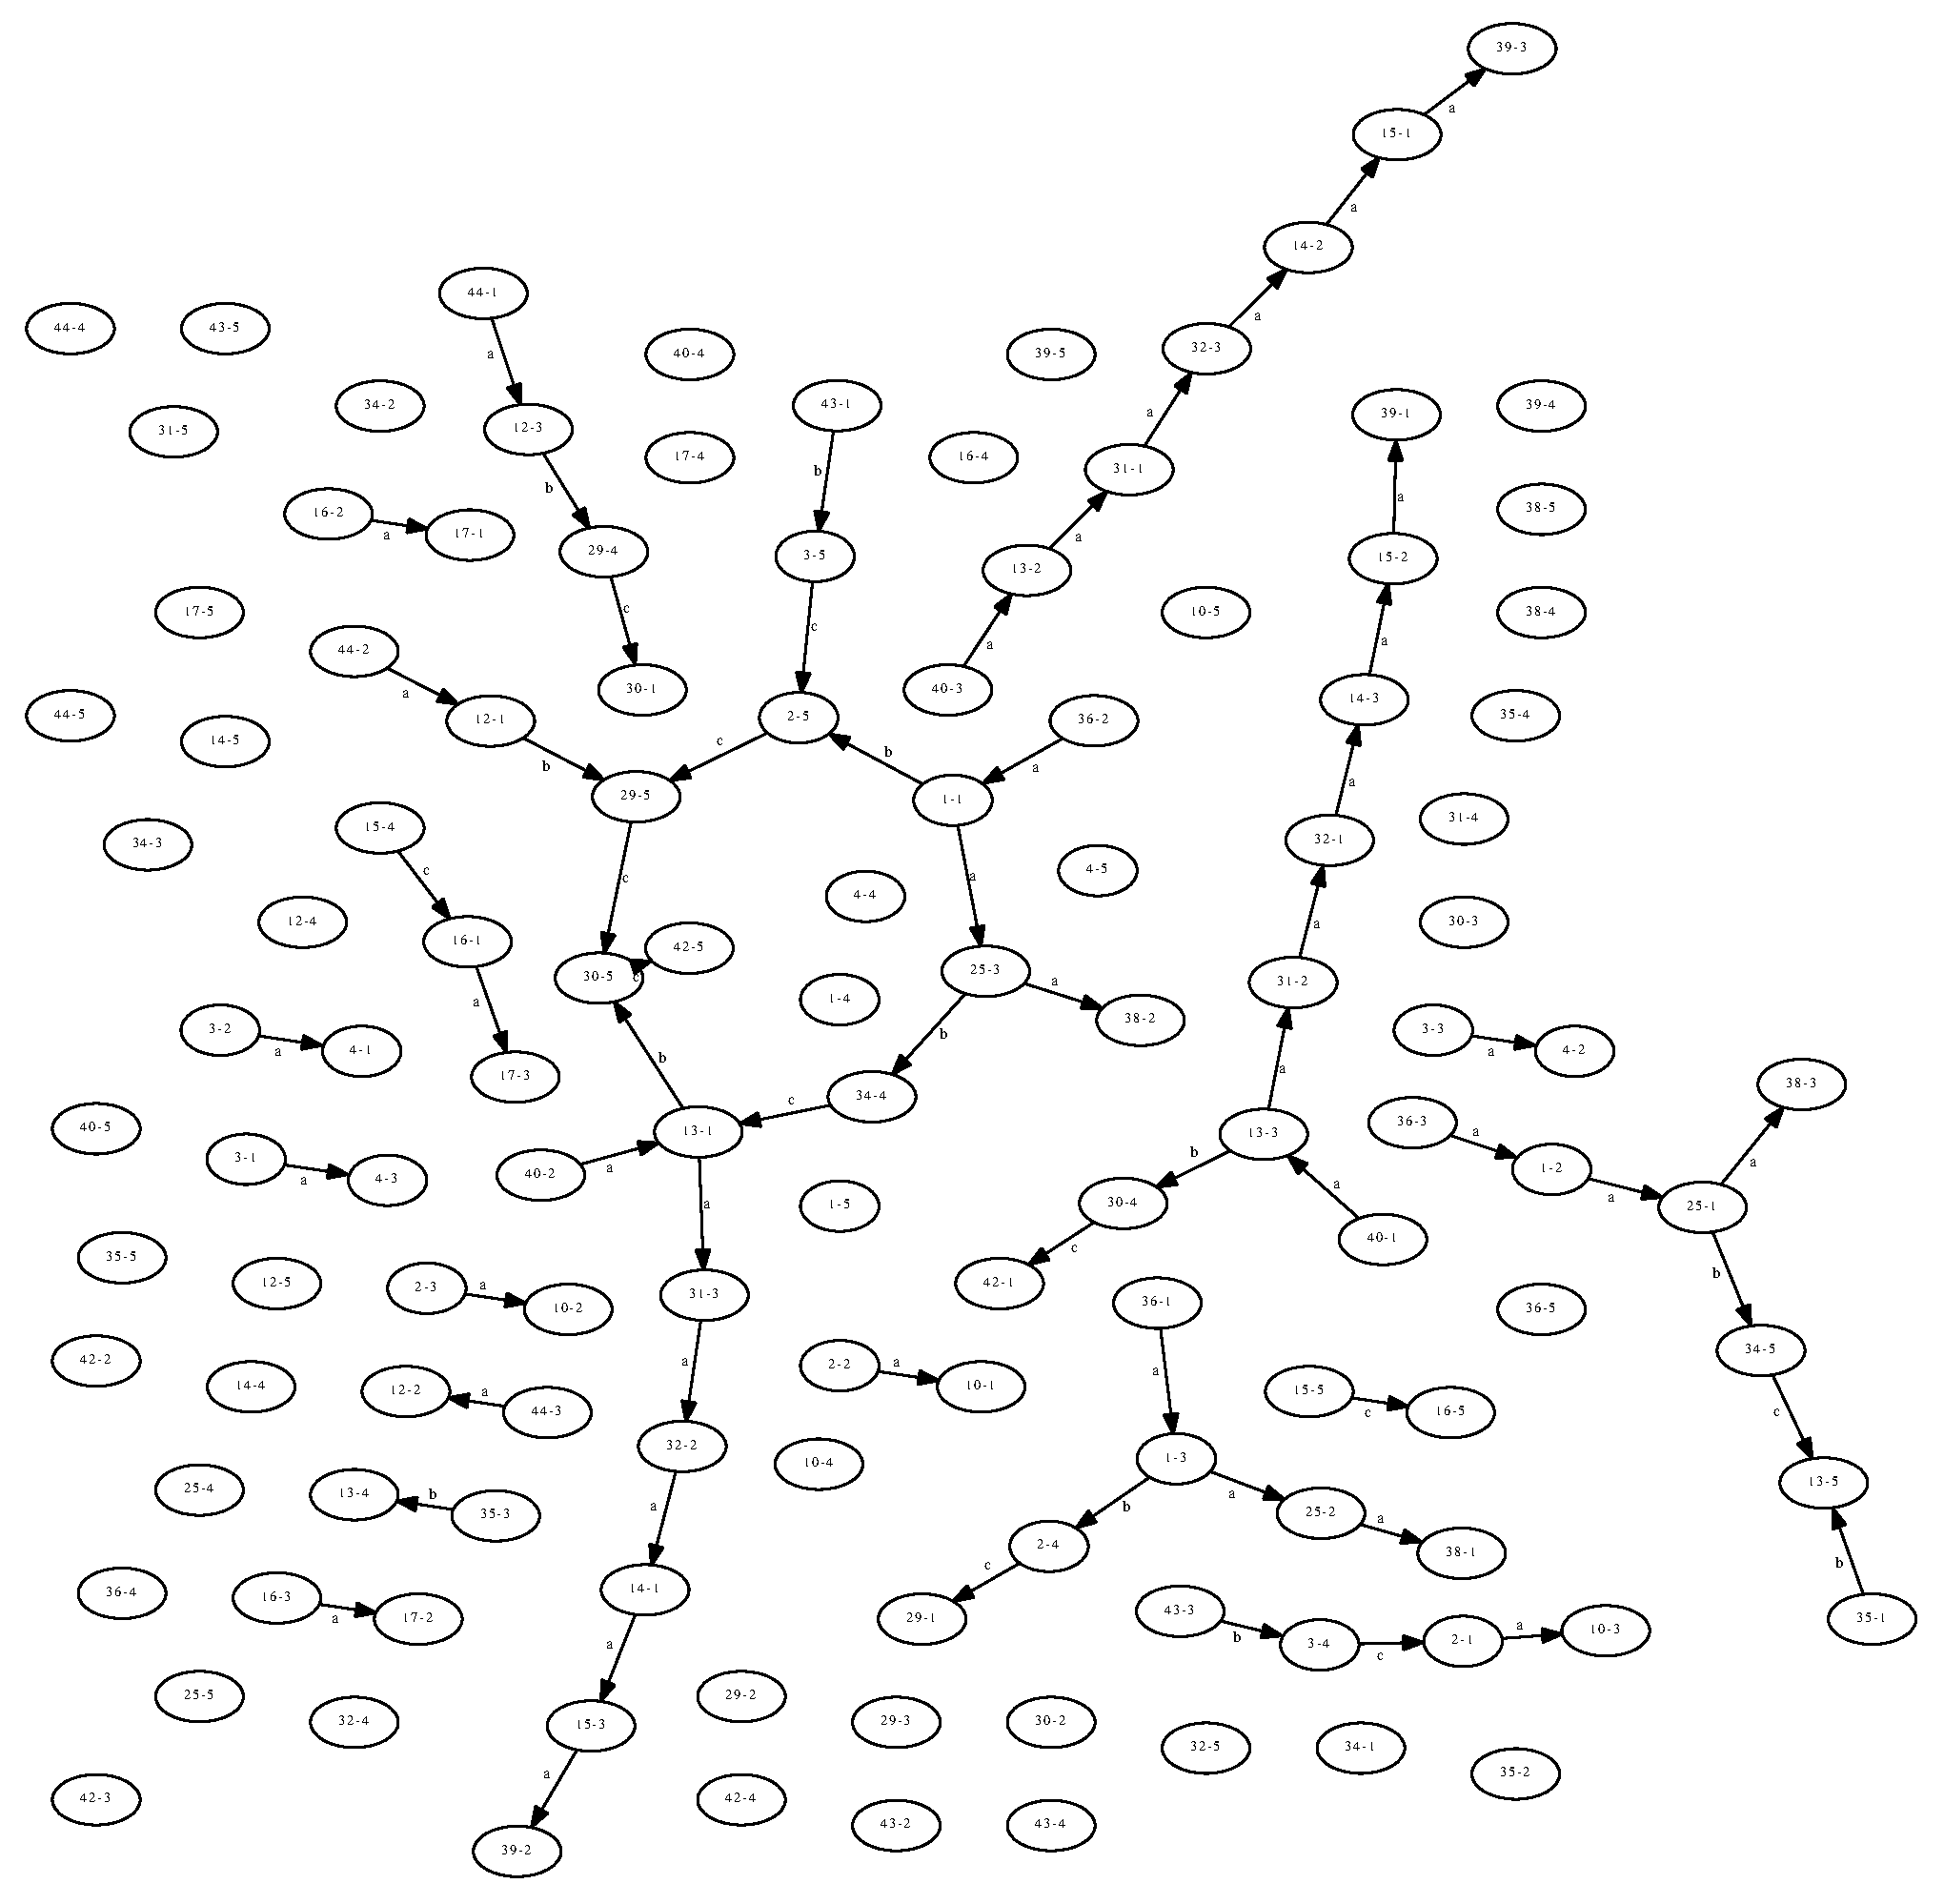
\includegraphics[scale=0.47, bb=0 0 1050 1030]{python/ex_K_f4-x-g.eps}
\caption{$\cP_4=\Theta_4\times \G_{A_1}$}
\label{fig:K_f4-x-g}
\end{center}
\end{figure}

\begin{comment}
\begin{figure}
\begin{center}
\psfrag{a}{\hspace{2pt}\small$x_1$}
\psfrag{a1}{\hspace*{-18pt}\small$x_1$}
\psfrag{a2}{\hspace*{-24pt}\raisebox{2pt}{\small$x_1$}}
\psfrag{a3}{\hspace*{2pt}\raisebox{-4pt}{\small$x_1$}}
\psfrag{b}{\hspace{2pt}\small$x_2$}
\psfrag{b1}{\hspace{2pt}\raisebox{-2pt}{\small$x_2$}}
\psfrag{b2}{\hspace{-12pt}\small$x_2$}
\psfrag{b3}{\hspace{-8pt}\raisebox{-8pt}{\small$x_2$}}
\psfrag{b4}{\hspace{-12pt}\raisebox{6pt}{\small$x_2$}}
\psfrag{c}{\hspace{2pt}\small$x_3$}
\psfrag{c1}{\hspace{-14pt}\raisebox{-2pt}{\small$x_3$}}
\psfrag{c2}{\hspace{6pt}\raisebox{-6pt}{\small$x_3$}}
\psfrag{c3}{\hspace{2pt}\raisebox{-4pt}{\small$x_3$}}
\psfrag{r}{\hspace{2pt}\small$y_1$}
\psfrag{r1}{\hspace{8pt}\small$y_1$}
\psfrag{s}{\hspace{2pt}\small$y_2$}
\psfrag{s1}{\hspace{-12pt}\raisebox{4pt}{\small$y_2$}}
\psfrag{t}{\hspace{2pt}\small$y_3$}
\psfrag{t1}{\hspace{8pt}\small$y_3$}
\psfrag{x}{\hspace{2pt}\small$z_1$}
\psfrag{x1}{\hspace{-15pt}\small$z_1$}
\psfrag{x2}{\hspace{-20pt}\raisebox{0pt}{\small$z_1$}}
\psfrag{x3}{\hspace{2pt}\raisebox{6pt}{\small$z_1$}}
\psfrag{y}{\hspace{2pt}\small$z_2$}
\psfrag{y1}{\hspace{-18pt}\small$z_2$}
\psfrag{y2}{\hspace{2pt}\raisebox{6pt}{\small$z_2$}}
 \psfrag{z}{\hspace{2pt}\small$z_3$}
\psfrag{z1}{\hspace{-16pt}\small$z_3$}
\psfrag{z2}{\hspace{-8pt}\raisebox{-6pt}{\small$z_3$}}
\psfrag{z3}{\hspace{-30pt}\small$z_3$}
\psfrag{u}{\hspace{2pt}\small $y_4$}
\psfrag{1}{\hspace{-1pt}\raisebox{-2pt}{\scriptsize $1$}}
\psfrag{2}{\hspace{-1pt}\raisebox{-2pt}{\scriptsize $2$}}
\psfrag{3}{\hspace{-1pt}\raisebox{-2pt}{\scriptsize $3$}}
\psfrag{4}{\hspace{-1pt}\raisebox{-2pt}{\scriptsize $4$}}
\psfrag{5}{\hspace{-1pt}\raisebox{-2pt}{\scriptsize $5$}}
\psfrag{6}{\hspace{-1pt}\raisebox{-2pt}{\scriptsize $6$}}
\psfrag{7}{\hspace{-1pt}\raisebox{-2pt}{\scriptsize $7$}}
\psfrag{8}{\hspace{-1pt}\raisebox{-2pt}{\scriptsize $8$}}
\psfrag{9}{\hspace{-1pt}\raisebox{-2pt}{\scriptsize $9$}}
\psfrag{10}{\hspace{-2pt}\raisebox{-2pt}{\scriptsize $10$}}
\psfrag{11}{\hspace{-2pt}\raisebox{-2pt}{\scriptsize $11$}}
\psfrag{12}{\hspace{-2pt}\raisebox{-2pt}{\scriptsize $12$}}
\psfrag{13}{\hspace{-2pt}\raisebox{-2pt}{\scriptsize $13$}}
\psfrag{14}{\hspace{-2pt}\raisebox{-2pt}{\scriptsize $14$}}
\psfrag{15}{\hspace{-2pt}\raisebox{-2pt}{\scriptsize $15$}}
\psfrag{16}{\hspace{-2pt}\raisebox{-2pt}{\scriptsize $16$}}
\psfrag{17}{\hspace{-2pt}\raisebox{-2pt}{\scriptsize $17$}}
\psfrag{18}{\hspace{-2pt}\raisebox{-2pt}{\scriptsize $18$}}
\psfrag{19}{\hspace{-2pt}\raisebox{-2pt}{\scriptsize $19$}}
\psfrag{20}{\hspace{-2pt}\raisebox{-2pt}{\scriptsize $20$}}
\psfrag{21}{\hspace{-2pt}\raisebox{-2pt}{\scriptsize $21$}}
\psfrag{22}{\hspace{-2pt}\raisebox{-2pt}{\scriptsize $22$}}
\psfrag{23}{\hspace{-2pt}\raisebox{-2pt}{\scriptsize $23$}}
\psfrag{24}{\hspace{-2pt}\raisebox{-2pt}{\scriptsize $24$}}
\psfrag{25}{\hspace{-2pt}\raisebox{-2pt}{\scriptsize $25$}}
\psfrag{26}{\hspace{-2pt}\raisebox{-2pt}{\scriptsize $26$}}
\psfrag{27}{\hspace{-2pt}\raisebox{-2pt}{\scriptsize $27$}}
\psfrag{28}{\hspace{-2pt}\raisebox{-2pt}{\scriptsize $28$}}
\psfrag{29}{\hspace{-2pt}\raisebox{-2pt}{\scriptsize $29$}}
\psfrag{30}{\hspace{-2pt}\raisebox{-2pt}{\scriptsize $30$}}
\psfrag{31}{\hspace{-2pt}\raisebox{-2pt}{\scriptsize $31$}}
\psfrag{32}{\hspace{-2pt}\raisebox{-2pt}{\scriptsize $32$}}
\psfrag{33}{\hspace{-2pt}\raisebox{-2pt}{\scriptsize $33$}}
\psfrag{34}{\hspace{-2pt}\raisebox{-2pt}{\scriptsize $34$}}
\psfrag{35}{\hspace{-2pt}\raisebox{-2pt}{\scriptsize $35$}}
\psfrag{36}{\hspace{-2pt}\raisebox{-2pt}{\scriptsize $36$}}
\psfrag{37}{\hspace{-2pt}\raisebox{-2pt}{\scriptsize $37$}}
\psfrag{38}{\hspace{-2pt}\raisebox{-2pt}{\scriptsize $38$}}
\psfrag{39}{\hspace{-2pt}\raisebox{-2pt}{\scriptsize $39$}}
\psfrag{40}{\hspace{-2pt}\raisebox{-2pt}{\scriptsize $40$}}
\psfrag{41}{\hspace{-2pt}\raisebox{-2pt}{\scriptsize $41$}}
\psfrag{42}{\hspace{-2pt}\raisebox{-2pt}{\scriptsize $42$}}
\psfrag{43}{\hspace{-2pt}\raisebox{-2pt}{\scriptsize $43$}}
\psfrag{44}{\hspace{-2pt}\raisebox{-2pt}{\scriptsize $44$}}
\psfrag{45}{\hspace{-2pt}\raisebox{-2pt}{\scriptsize $45$}}
\psfrag{46}{\hspace{-2pt}\raisebox{-2pt}{\scriptsize $46$}}
\psfrag{47}{\hspace{-2pt}\raisebox{-2pt}{\scriptsize $47$}}
\psfrag{48}{\hspace{-2pt}\raisebox{-2pt}{\scriptsize $48$}}
\psfrag{49}{\hspace{-2pt}\raisebox{-2pt}{\scriptsize $49$}}
%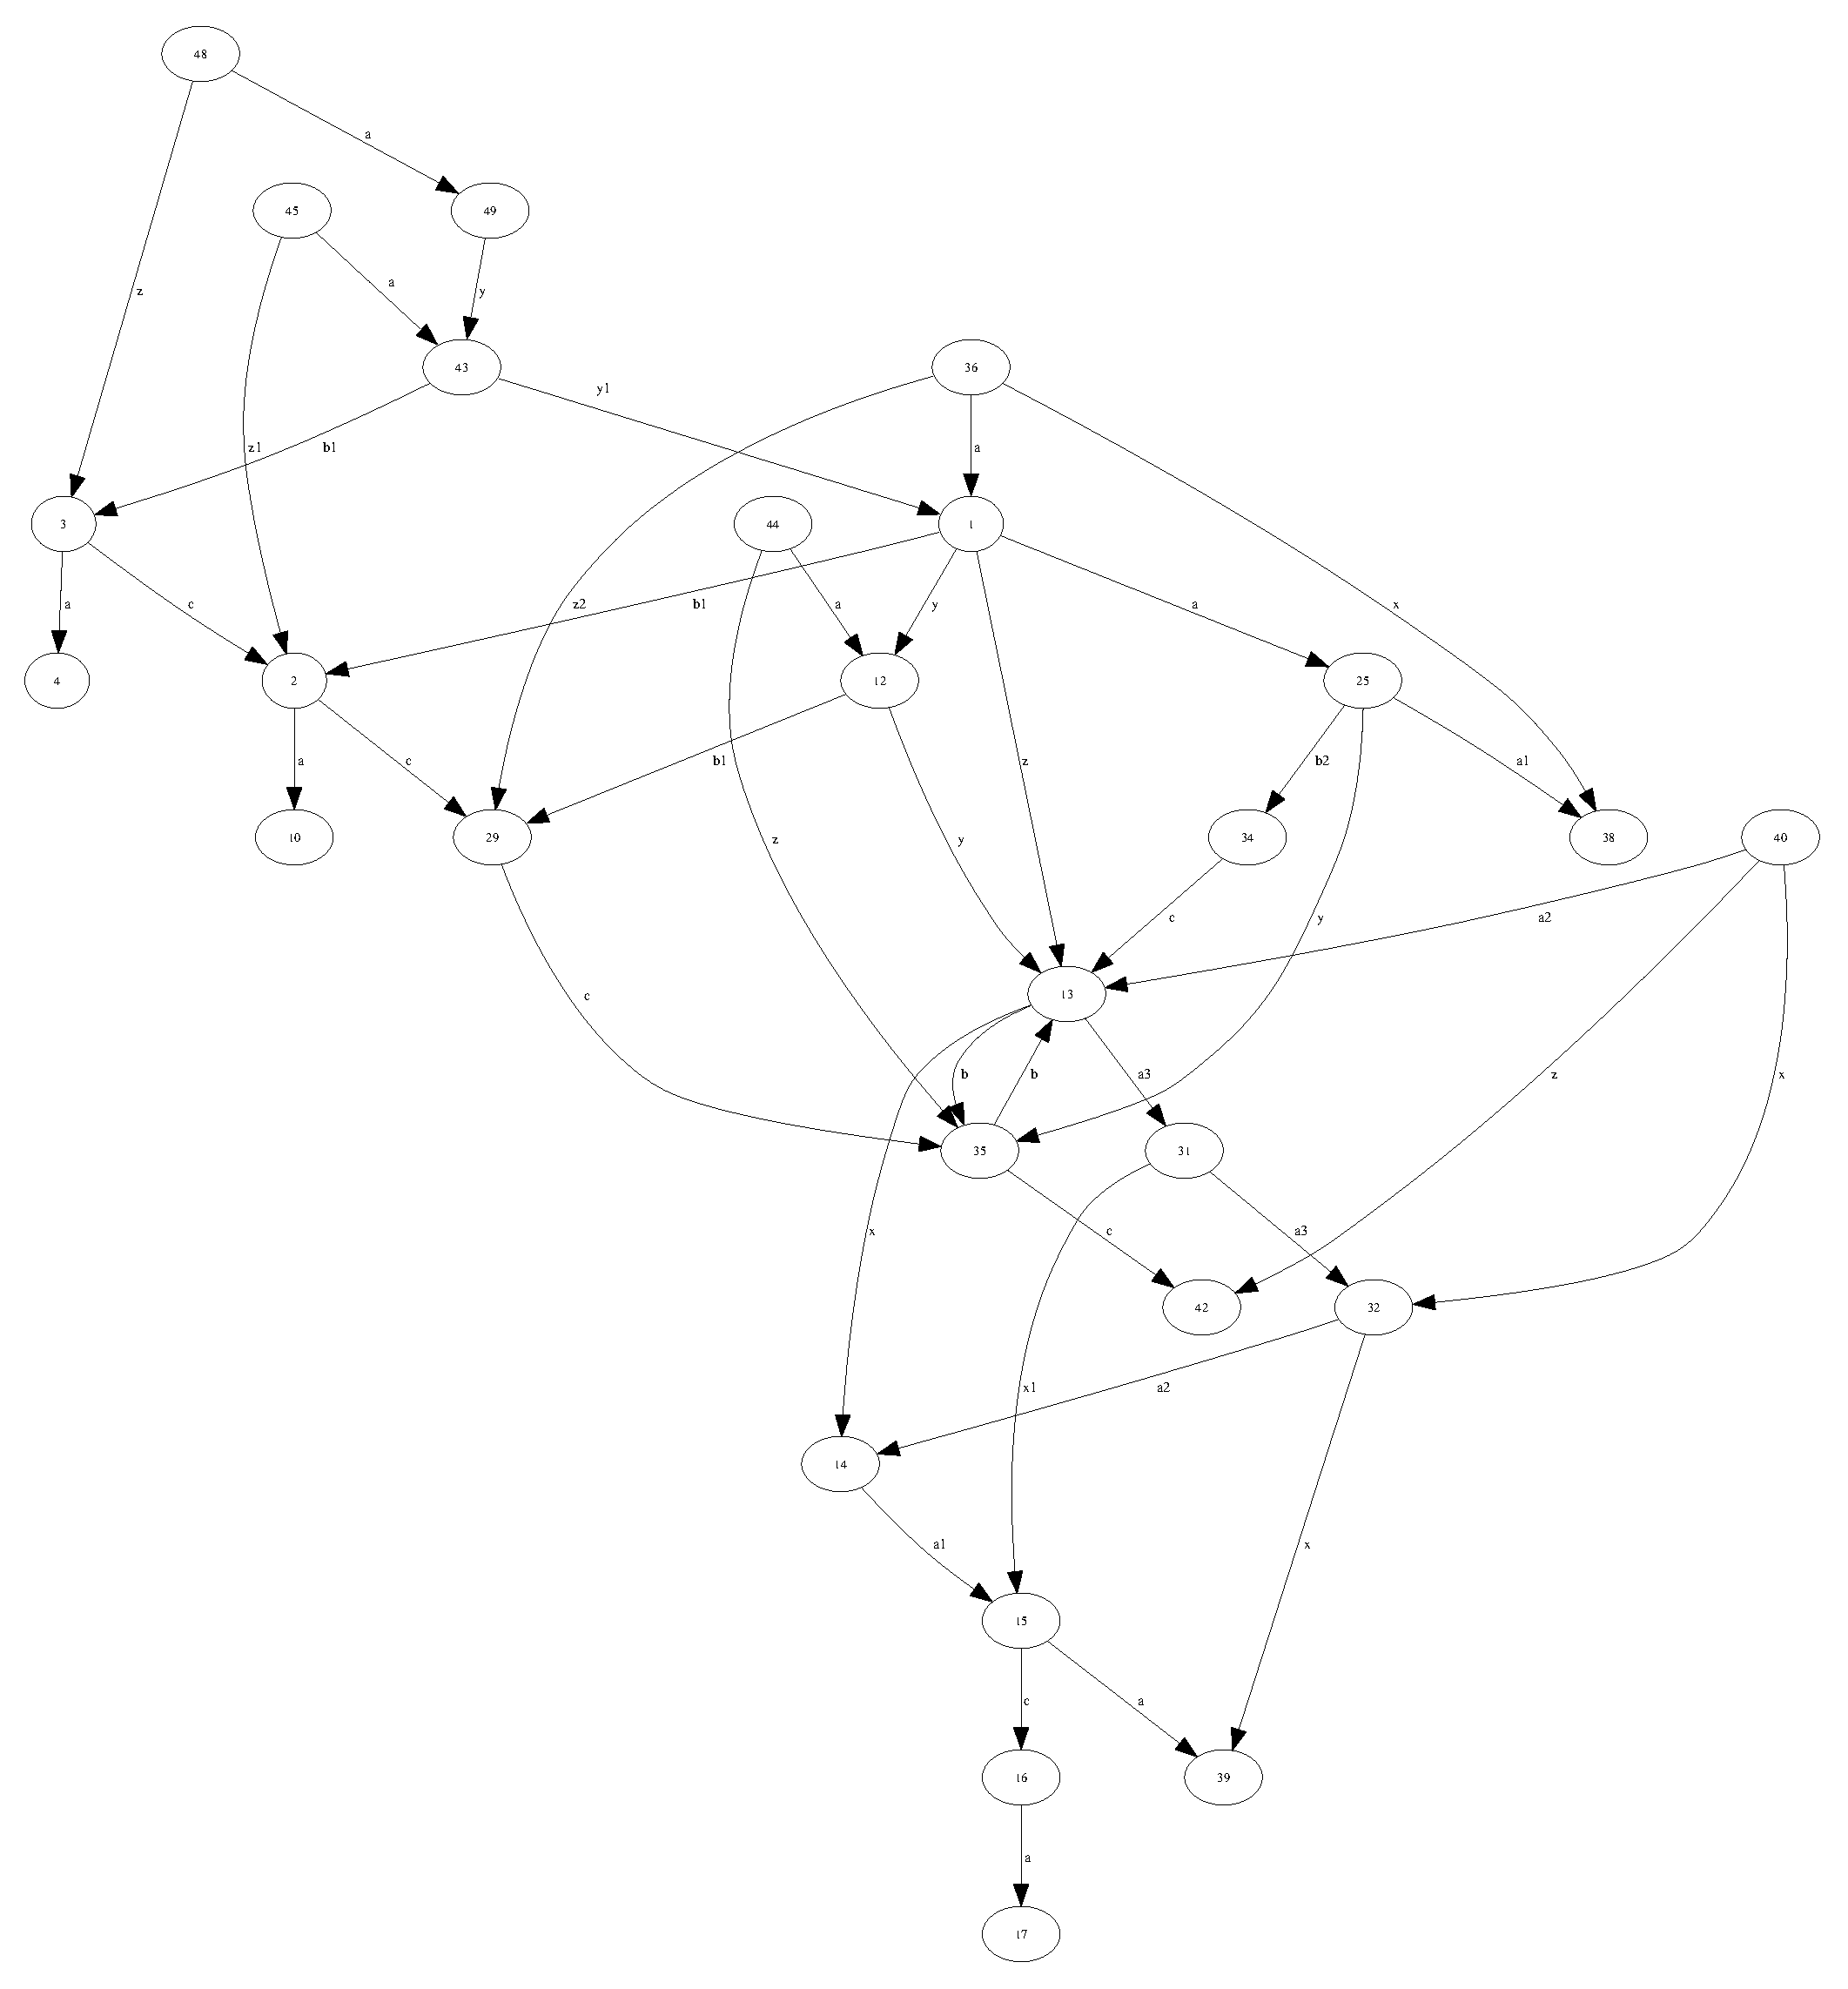
\includegraphics[scale=0.5]{python/ex_K_f5.eps}
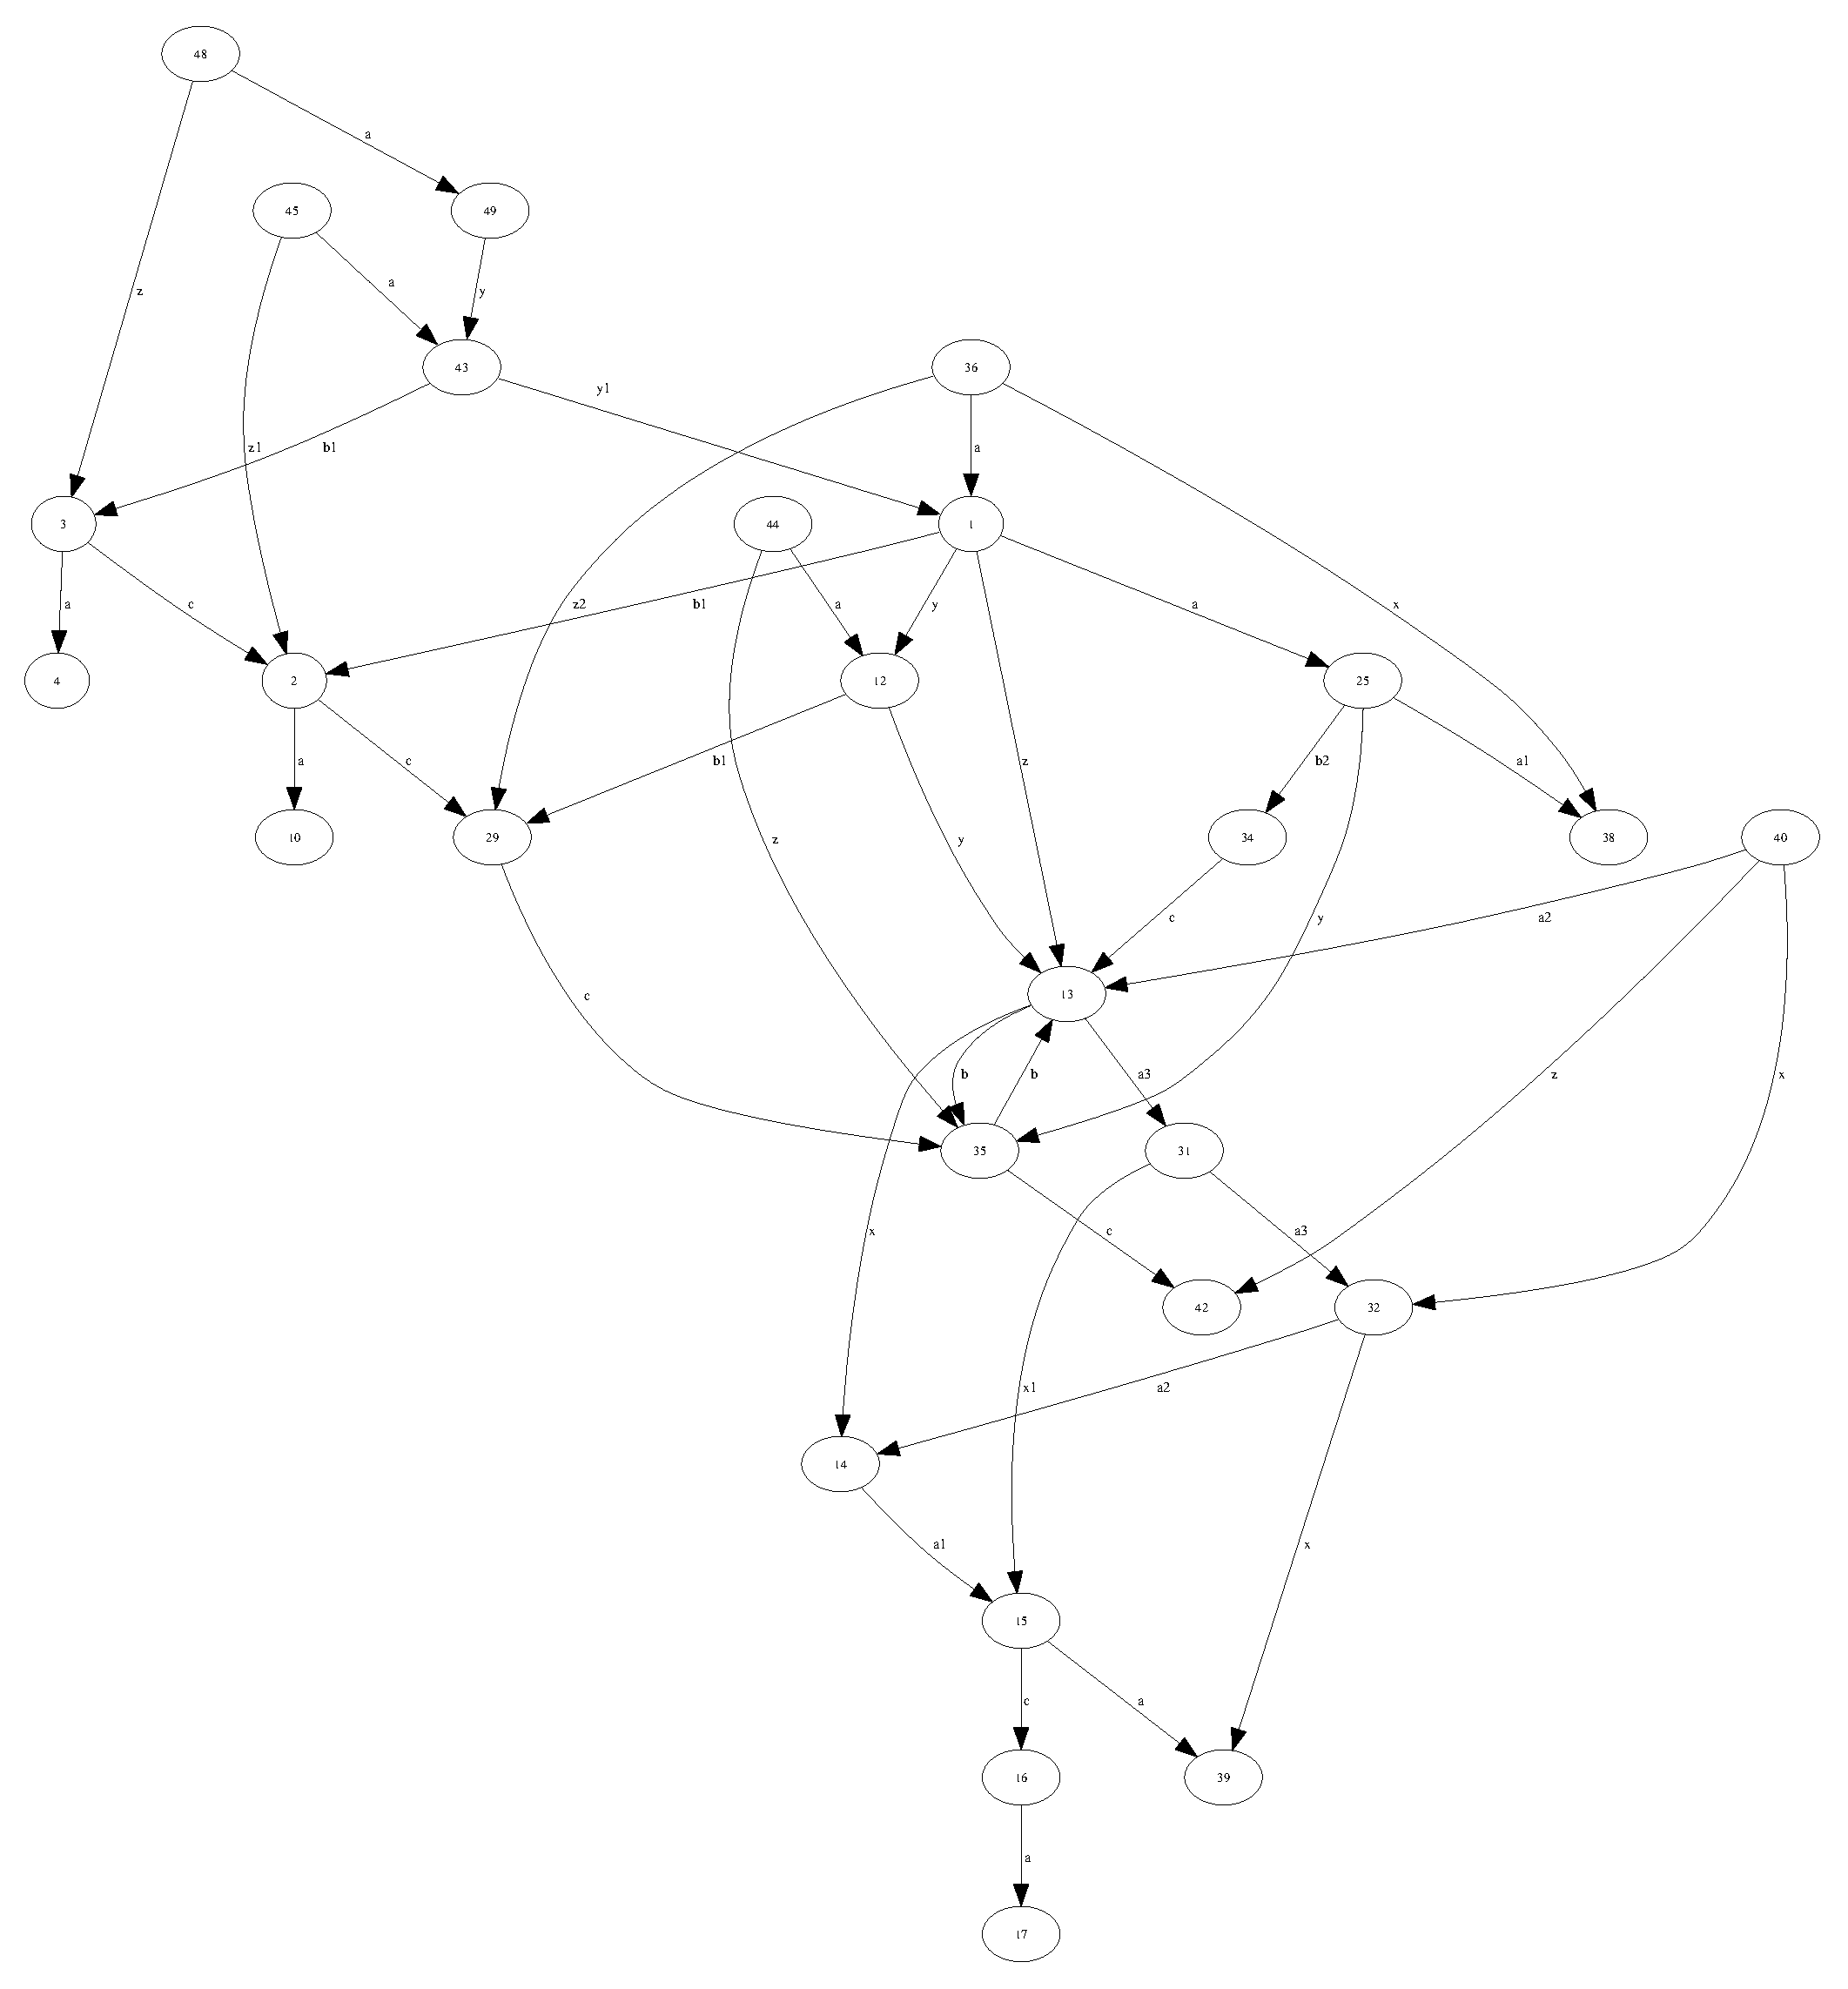
\includegraphics[scale=0.5, bb=36 36 892 854]{python/ex_K_f5.eps}
\caption{$\Theta_5$}
\label{fig:K_f5}
\end{center}
\end{figure}
\end{comment}

\begin{figure}
\begin{center}
\psfrag{a}{\hspace{2pt}\small$x_1$}
\psfrag{a1}{\hspace*{-20pt}\small$x_1$}
\psfrag{a2}{\hspace*{0pt}\raisebox{-6pt}{\small$x_1$}}
\psfrag{a3}{\hspace*{-4pt}\raisebox{6pt}{\small$x_1$}}
\psfrag{b}{\hspace{2pt}\small$x_2$}
\psfrag{b1}{\hspace{-8pt}\raisebox{-6pt}{\small$x_2$}}
\psfrag{b2}{\hspace{-16pt}\small$x_2$}
\psfrag{b3}{\hspace{-8pt}\raisebox{-8pt}{\small$x_2$}}
\psfrag{b4}{\hspace{-12pt}\raisebox{6pt}{\small$x_2$}}
\psfrag{c}{\hspace{2pt}\small$x_3$}
\psfrag{c1}{\hspace{-14pt}\raisebox{-2pt}{\small$x_3$}}
\psfrag{c2}{\hspace{6pt}\raisebox{-6pt}{\small$x_3$}}
\psfrag{c3}{\hspace{2pt}\raisebox{-4pt}{\small$x_3$}}
\psfrag{r}{\hspace{2pt}\small$y_1$}
\psfrag{r1}{\hspace{8pt}\small$y_1$}
\psfrag{s}{\hspace{2pt}\small$y_2$}
\psfrag{s1}{\hspace{-12pt}\raisebox{4pt}{\small$y_2$}}
\psfrag{t}{\hspace{2pt}\small$y_3$}
\psfrag{t1}{\hspace{8pt}\small$y_3$}
\psfrag{x}{\hspace{2pt}\small$z_1$}
\psfrag{x1}{\hspace{-10pt}\raisebox{10pt}{\small$z_1$}}
\psfrag{x2}{\hspace{-20pt}\raisebox{0pt}{\small$z_1$}}
\psfrag{x3}{\hspace{2pt}\raisebox{6pt}{\small$z_1$}}
\psfrag{y}{\hspace{2pt}\small$z_2$}
\psfrag{y1}{\hspace{-28pt}\raisebox{12pt}{\small$z_2$}}
\psfrag{y2}{\hspace{2pt}\raisebox{6pt}{\small$z_2$}}
 \psfrag{z}{\hspace{2pt}\small$z_3$}
\psfrag{z1}{\hspace{5pt}\raisebox{16pt}{\small$z_3$}}
\psfrag{z2}{\hspace{-5pt}\raisebox{16pt}{\small$z_3$}}
\psfrag{z3}{\hspace{-30pt}\small$z_3$}
\psfrag{u}{\hspace{2pt}\small $y_4$}
\psfrag{1}{\hspace{-1pt}\raisebox{-2pt}{\scriptsize $1$}}
\psfrag{2}{\hspace{-1pt}\raisebox{-2pt}{\scriptsize $2$}}
\psfrag{3}{\hspace{-1pt}\raisebox{-2pt}{\scriptsize $3$}}
\psfrag{4}{\hspace{-1pt}\raisebox{-2pt}{\scriptsize $4$}}
\psfrag{5}{\hspace{-1pt}\raisebox{-2pt}{\scriptsize $5$}}
\psfrag{6}{\hspace{-1pt}\raisebox{-2pt}{\scriptsize $6$}}
\psfrag{7}{\hspace{-1pt}\raisebox{-2pt}{\scriptsize $7$}}
\psfrag{8}{\hspace{-1pt}\raisebox{-2pt}{\scriptsize $8$}}
\psfrag{9}{\hspace{-1pt}\raisebox{-2pt}{\scriptsize $9$}}
\psfrag{10}{\hspace{-2pt}\raisebox{-2pt}{\scriptsize $10$}}
\psfrag{11}{\hspace{-2pt}\raisebox{-2pt}{\scriptsize $11$}}
\psfrag{12}{\hspace{-2pt}\raisebox{-2pt}{\scriptsize $12$}}
\psfrag{13}{\hspace{-2pt}\raisebox{-2pt}{\scriptsize $13$}}
\psfrag{14}{\hspace{-2pt}\raisebox{-2pt}{\scriptsize $14$}}
\psfrag{15}{\hspace{-2pt}\raisebox{-2pt}{\scriptsize $15$}}
\psfrag{16}{\hspace{-2pt}\raisebox{-2pt}{\scriptsize $16$}}
\psfrag{17}{\hspace{-2pt}\raisebox{-2pt}{\scriptsize $17$}}
\psfrag{18}{\hspace{-2pt}\raisebox{-2pt}{\scriptsize $18$}}
\psfrag{19}{\hspace{-2pt}\raisebox{-2pt}{\scriptsize $19$}}
\psfrag{20}{\hspace{-2pt}\raisebox{-2pt}{\scriptsize $20$}}
\psfrag{21}{\hspace{-2pt}\raisebox{-2pt}{\scriptsize $21$}}
\psfrag{22}{\hspace{-2pt}\raisebox{-2pt}{\scriptsize $22$}}
\psfrag{23}{\hspace{-2pt}\raisebox{-2pt}{\scriptsize $23$}}
\psfrag{24}{\hspace{-2pt}\raisebox{-2pt}{\scriptsize $24$}}
\psfrag{25}{\hspace{-2pt}\raisebox{-2pt}{\scriptsize $25$}}
\psfrag{26}{\hspace{-2pt}\raisebox{-2pt}{\scriptsize $26$}}
\psfrag{27}{\hspace{-2pt}\raisebox{-2pt}{\scriptsize $27$}}
\psfrag{28}{\hspace{-2pt}\raisebox{-2pt}{\scriptsize $28$}}
\psfrag{29}{\hspace{-2pt}\raisebox{-2pt}{\scriptsize $29$}}
\psfrag{30}{\hspace{-2pt}\raisebox{-2pt}{\scriptsize $30$}}
\psfrag{31}{\hspace{-2pt}\raisebox{-2pt}{\scriptsize $31$}}
\psfrag{32}{\hspace{-2pt}\raisebox{-2pt}{\scriptsize $32$}}
\psfrag{33}{\hspace{-2pt}\raisebox{-2pt}{\scriptsize $33$}}
\psfrag{34}{\hspace{-2pt}\raisebox{-2pt}{\scriptsize $34$}}
\psfrag{35}{\hspace{-2pt}\raisebox{-2pt}{\scriptsize $35$}}
\psfrag{36}{\hspace{-2pt}\raisebox{-2pt}{\scriptsize $36$}}
\psfrag{37}{\hspace{-2pt}\raisebox{-2pt}{\scriptsize $37$}}
\psfrag{38}{\hspace{-2pt}\raisebox{-2pt}{\scriptsize $38$}}
\psfrag{39}{\hspace{-2pt}\raisebox{-2pt}{\scriptsize $39$}}
\psfrag{40}{\hspace{-2pt}\raisebox{-2pt}{\scriptsize $40$}}
\psfrag{41}{\hspace{-2pt}\raisebox{-2pt}{\scriptsize $41$}}
\psfrag{42}{\hspace{-2pt}\raisebox{-2pt}{\scriptsize $42$}}
\psfrag{43}{\hspace{-2pt}\raisebox{-2pt}{\scriptsize $43$}}
\psfrag{44}{\hspace{-2pt}\raisebox{-2pt}{\scriptsize $44$}}
\psfrag{45}{\hspace{-2pt}\raisebox{-2pt}{\scriptsize $45$}}
\psfrag{46}{\hspace{-2pt}\raisebox{-2pt}{\scriptsize $46$}}
\psfrag{47}{\hspace{-2pt}\raisebox{-2pt}{\scriptsize $47$}}
\psfrag{48}{\hspace{-2pt}\raisebox{-2pt}{\scriptsize $48$}}
\psfrag{49}{\hspace{-2pt}\raisebox{-2pt}{\scriptsize $49$}}
%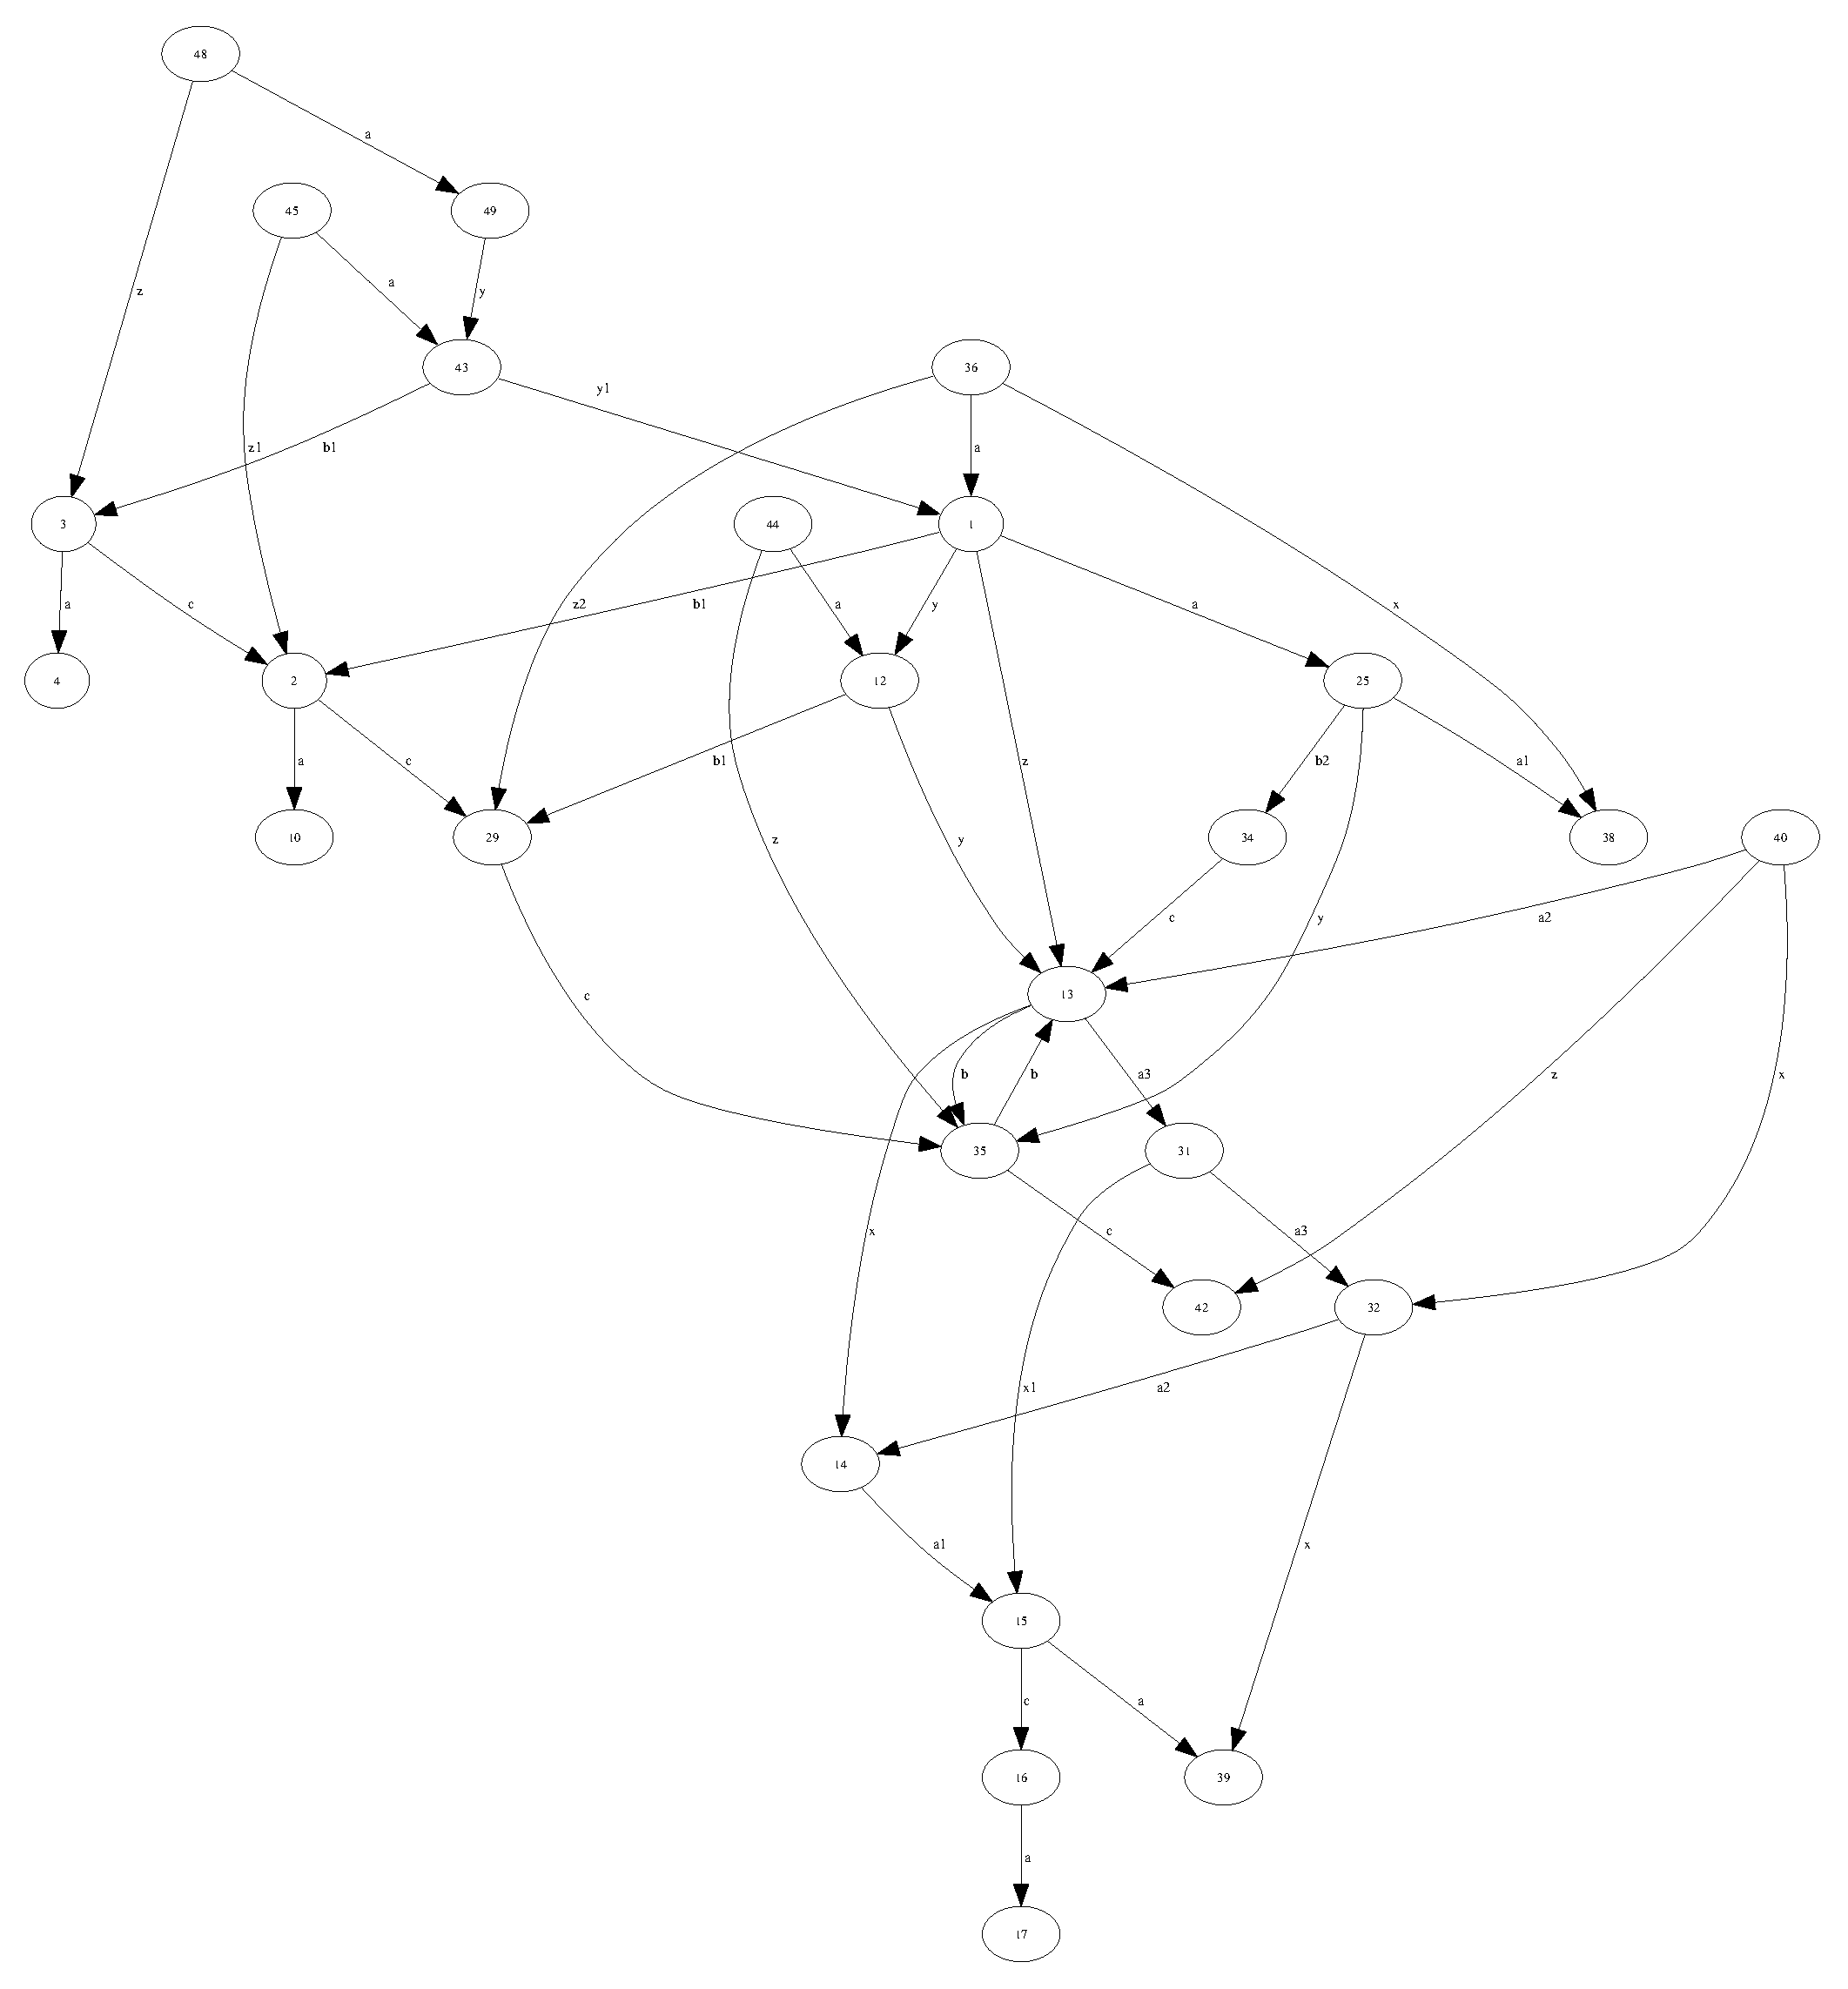
\includegraphics[scale=0.5]{python/ex_K_f5.eps}
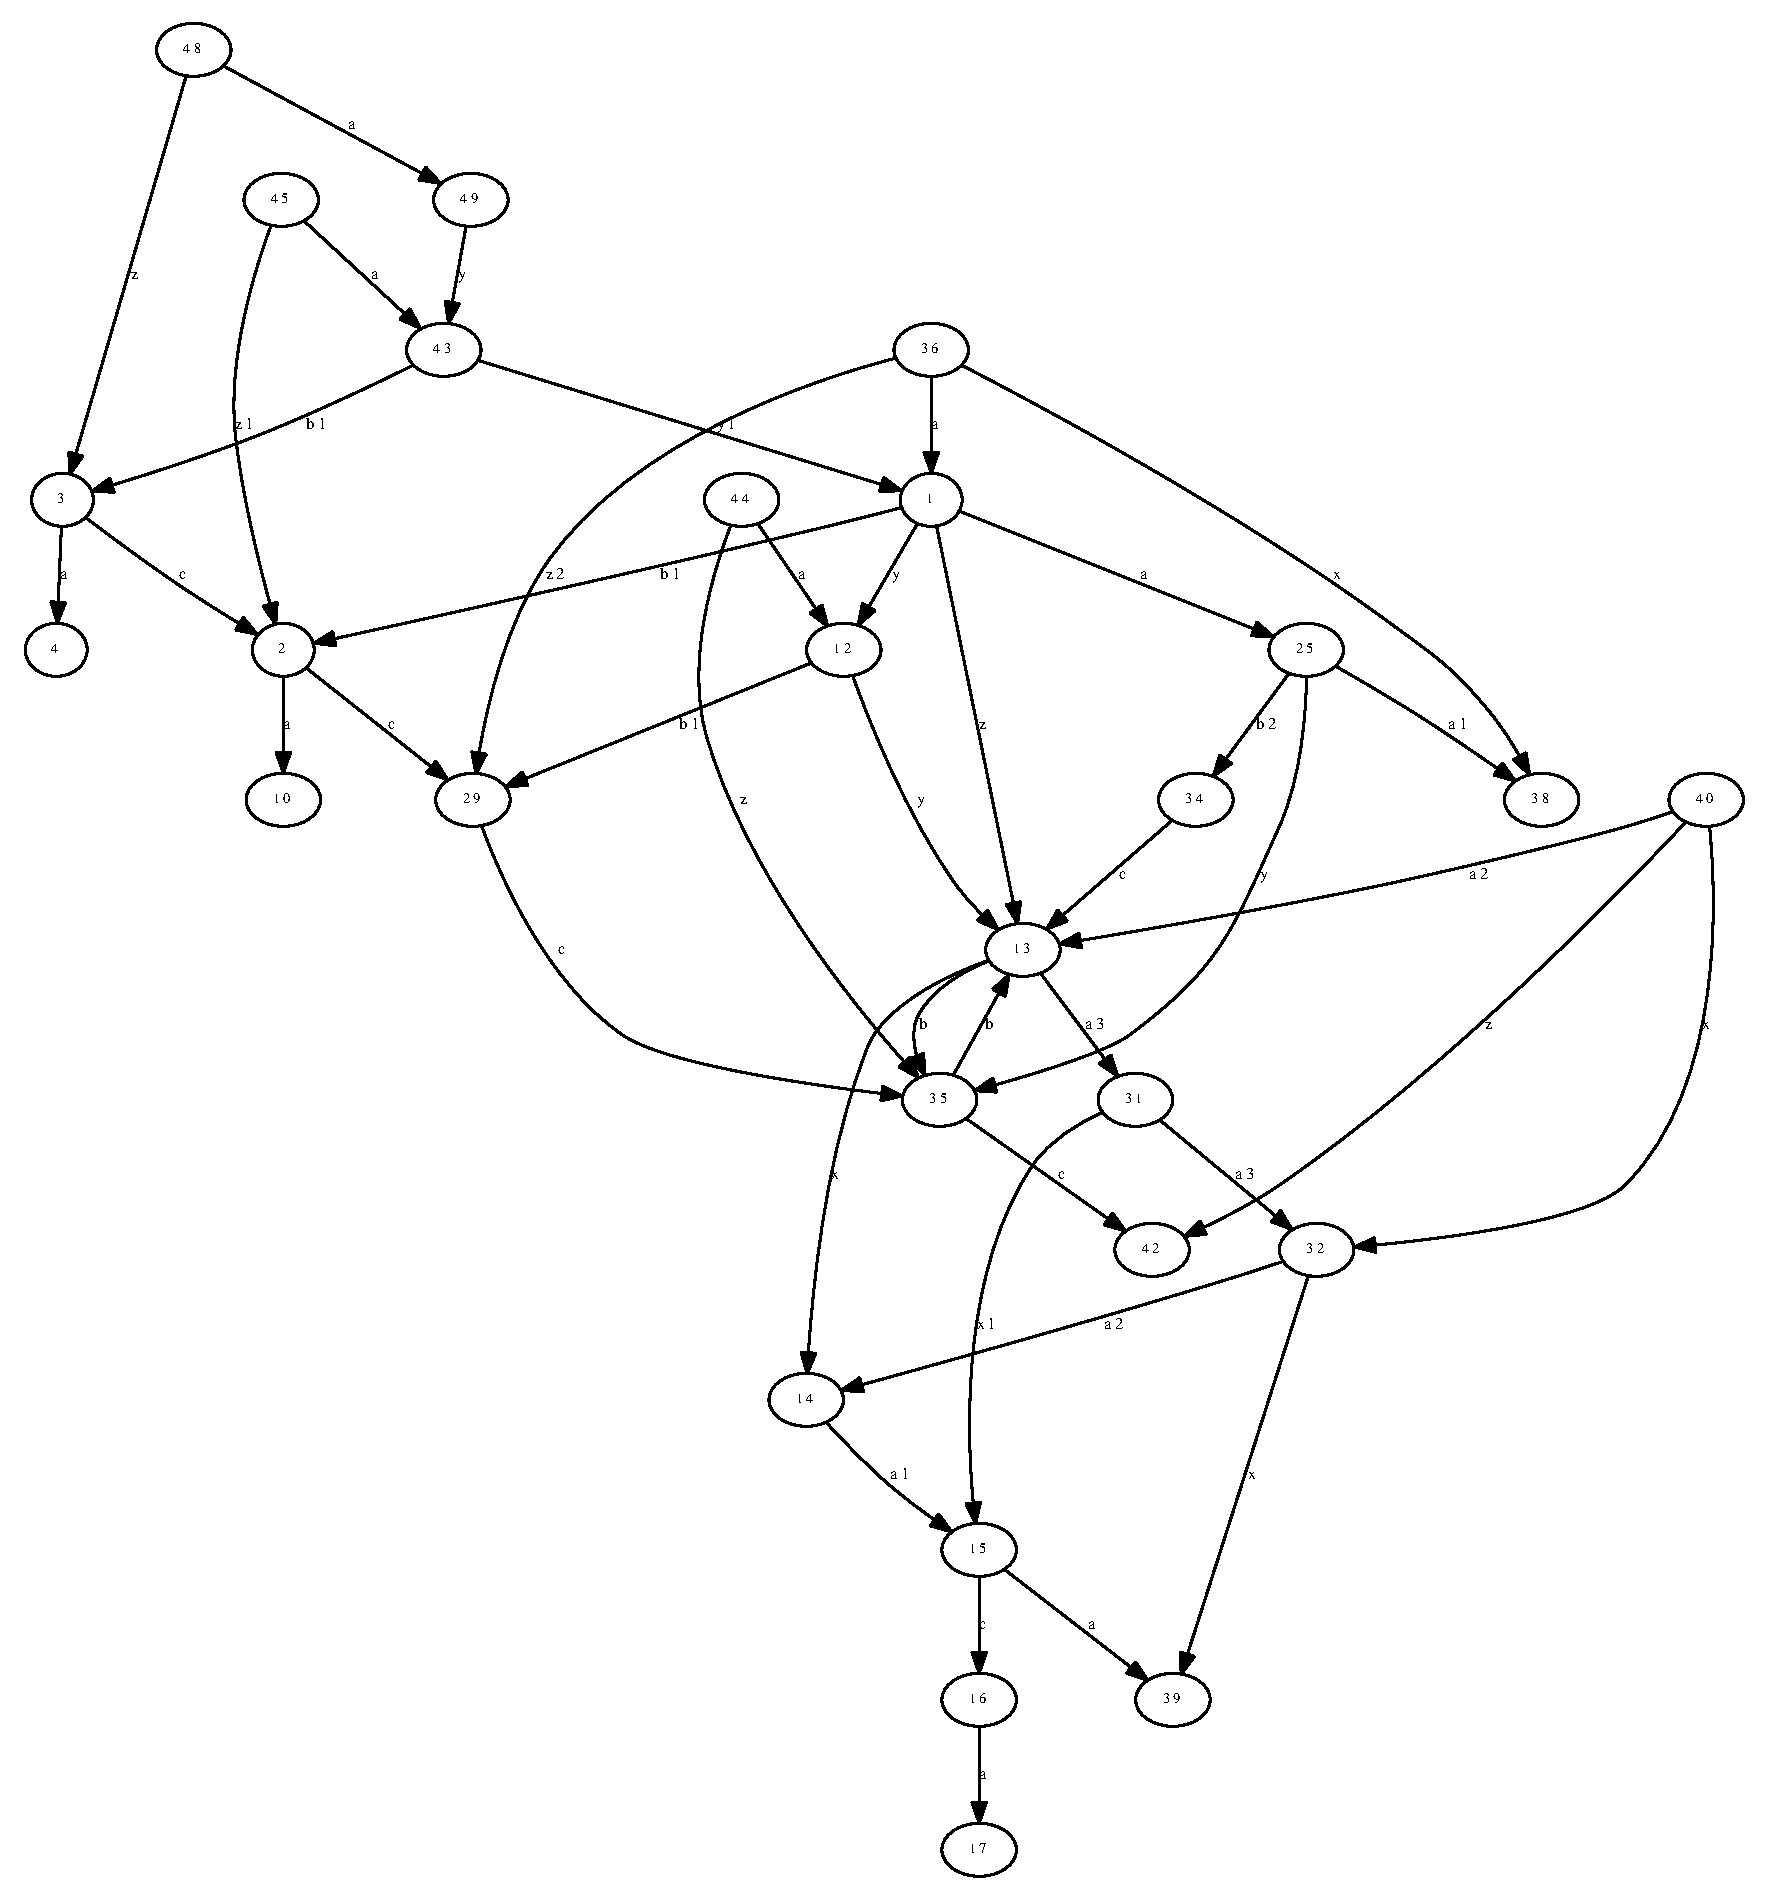
\includegraphics[scale=0.5, bb=36 36 892 854]{python/ex_K_f5_new.eps}
\caption{$\Theta_5$}
\label{fig:K_f5}
\end{center}
\end{figure}

\begin{figure}
\begin{center}
\psfrag{1-1}{\hspace{-4pt}\raisebox{-2pt}{\scriptsize $1,1$}}
\psfrag{1-2}{\hspace{-4pt}\raisebox{-2pt}{\scriptsize $1,2$}}
\psfrag{1-3}{\hspace{-4pt}\raisebox{-2pt}{\scriptsize $1,3$}}
\psfrag{1-4}{\hspace{-4pt}\raisebox{-2pt}{\scriptsize $1,4$}}
\psfrag{1-5}{\hspace{-4pt}\raisebox{-2pt}{\scriptsize $1,5$}}
\psfrag{1-6}{\hspace{-4pt}\raisebox{-2pt}{\scriptsize $1,6$}}
\psfrag{1-7}{\hspace{-4pt}\raisebox{-2pt}{\scriptsize $1,7$}}
\psfrag{1-8}{\hspace{-4pt}\raisebox{-2pt}{\scriptsize $1,8$}}
\psfrag{1-9}{\hspace{-4pt}\raisebox{-2pt}{\scriptsize $1,9$}}
\psfrag{2-1}{\hspace{-4pt}\raisebox{-2pt}{\scriptsize $2,1$}}
\psfrag{2-2}{\hspace{-4pt}\raisebox{-2pt}{\scriptsize $2,2$}}
\psfrag{2-3}{\hspace{-4pt}\raisebox{-2pt}{\scriptsize $2,3$}}
\psfrag{2-4}{\hspace{-4pt}\raisebox{-2pt}{\scriptsize $2,4$}}
\psfrag{2-5}{\hspace{-4pt}\raisebox{-2pt}{\scriptsize $2,5$}}
\psfrag{2-6}{\hspace{-4pt}\raisebox{-2pt}{\scriptsize $2,6$}}
\psfrag{2-7}{\hspace{-4pt}\raisebox{-2pt}{\scriptsize $2,7$}}
\psfrag{2-8}{\hspace{-4pt}\raisebox{-2pt}{\scriptsize $2,8$}}
\psfrag{2-9}{\hspace{-4pt}\raisebox{-2pt}{\scriptsize $2,9$}}
\psfrag{3-1}{\hspace{-4pt}\raisebox{-2pt}{\scriptsize $3,1$}}
\psfrag{3-2}{\hspace{-4pt}\raisebox{-2pt}{\scriptsize $3,2$}}
\psfrag{3-3}{\hspace{-4pt}\raisebox{-2pt}{\scriptsize $3,3$}}
\psfrag{3-4}{\hspace{-4pt}\raisebox{-2pt}{\scriptsize $3,4$}}
\psfrag{3-5}{\hspace{-4pt}\raisebox{-2pt}{\scriptsize $3,5$}}
\psfrag{3-6}{\hspace{-4pt}\raisebox{-2pt}{\scriptsize $3,6$}}
\psfrag{3-7}{\hspace{-4pt}\raisebox{-2pt}{\scriptsize $3,7$}}
\psfrag{3-8}{\hspace{-4pt}\raisebox{-2pt}{\scriptsize $3,8$}}
\psfrag{3-9}{\hspace{-4pt}\raisebox{-2pt}{\scriptsize $3,9$}}
\psfrag{4-1}{\hspace{-4pt}\raisebox{-2pt}{\scriptsize $4,1$}}
\psfrag{4-2}{\hspace{-4pt}\raisebox{-2pt}{\scriptsize $4,2$}}
\psfrag{4-3}{\hspace{-4pt}\raisebox{-2pt}{\scriptsize $4,3$}}
\psfrag{4-4}{\hspace{-4pt}\raisebox{-2pt}{\scriptsize $4,4$}}
\psfrag{4-5}{\hspace{-4pt}\raisebox{-2pt}{\scriptsize $4,5$}}
\psfrag{4-6}{\hspace{-4pt}\raisebox{-2pt}{\scriptsize $4,6$}}
\psfrag{4-7}{\hspace{-4pt}\raisebox{-2pt}{\scriptsize $4,7$}}
\psfrag{4-8}{\hspace{-4pt}\raisebox{-2pt}{\scriptsize $4,8$}}
\psfrag{4-9}{\hspace{-4pt}\raisebox{-2pt}{\scriptsize $4,9$}}
\psfrag{5-1}{\hspace{-4pt}\raisebox{-2pt}{\scriptsize $5,1$}}
\psfrag{5-2}{\hspace{-4pt}\raisebox{-2pt}{\scriptsize $5,2$}}
\psfrag{5-3}{\hspace{-4pt}\raisebox{-2pt}{\scriptsize $5,3$}}
\psfrag{5-4}{\hspace{-4pt}\raisebox{-2pt}{\scriptsize $5,4$}}
\psfrag{5-5}{\hspace{-4pt}\raisebox{-2pt}{\scriptsize $5,5$}}
\psfrag{5-6}{\hspace{-4pt}\raisebox{-2pt}{\scriptsize $5,6$}}
\psfrag{5-7}{\hspace{-4pt}\raisebox{-2pt}{\scriptsize $5,7$}}
\psfrag{5-8}{\hspace{-4pt}\raisebox{-2pt}{\scriptsize $5,8$}}
\psfrag{5-9}{\hspace{-4pt}\raisebox{-2pt}{\scriptsize $5,9$}}
\psfrag{6-1}{\hspace{-4pt}\raisebox{-2pt}{\scriptsize $6,1$}}
\psfrag{6-2}{\hspace{-4pt}\raisebox{-2pt}{\scriptsize $6,2$}}
\psfrag{6-3}{\hspace{-4pt}\raisebox{-2pt}{\scriptsize $6,3$}}
\psfrag{6-4}{\hspace{-4pt}\raisebox{-2pt}{\scriptsize $6,4$}}
\psfrag{6-5}{\hspace{-4pt}\raisebox{-2pt}{\scriptsize $6,5$}}
\psfrag{6-6}{\hspace{-4pt}\raisebox{-2pt}{\scriptsize $6,6$}}
\psfrag{6-7}{\hspace{-4pt}\raisebox{-2pt}{\scriptsize $6,7$}}
\psfrag{6-8}{\hspace{-4pt}\raisebox{-2pt}{\scriptsize $6,8$}}
\psfrag{6-9}{\hspace{-4pt}\raisebox{-2pt}{\scriptsize $6,9$}}
\psfrag{7-1}{\hspace{-4pt}\raisebox{-2pt}{\scriptsize $7,1$}}
\psfrag{7-2}{\hspace{-4pt}\raisebox{-2pt}{\scriptsize $7,2$}}
\psfrag{7-3}{\hspace{-4pt}\raisebox{-2pt}{\scriptsize $7,3$}}
\psfrag{7-4}{\hspace{-4pt}\raisebox{-2pt}{\scriptsize $7,4$}}
\psfrag{7-5}{\hspace{-4pt}\raisebox{-2pt}{\scriptsize $7,5$}}
\psfrag{7-6}{\hspace{-4pt}\raisebox{-2pt}{\scriptsize $7,6$}}
\psfrag{7-7}{\hspace{-4pt}\raisebox{-2pt}{\scriptsize $7,7$}}
\psfrag{7-8}{\hspace{-4pt}\raisebox{-2pt}{\scriptsize $7,8$}}
\psfrag{7-9}{\hspace{-4pt}\raisebox{-2pt}{\scriptsize $7,9$}}
\psfrag{8-1}{\hspace{-4pt}\raisebox{-2pt}{\scriptsize $8,1$}}
\psfrag{8-2}{\hspace{-4pt}\raisebox{-2pt}{\scriptsize $8,2$}}
\psfrag{8-3}{\hspace{-4pt}\raisebox{-2pt}{\scriptsize $8,3$}}
\psfrag{8-4}{\hspace{-4pt}\raisebox{-2pt}{\scriptsize $8,4$}}
\psfrag{8-5}{\hspace{-4pt}\raisebox{-2pt}{\scriptsize $8,5$}}
\psfrag{8-6}{\hspace{-4pt}\raisebox{-2pt}{\scriptsize $8,6$}}
\psfrag{8-7}{\hspace{-4pt}\raisebox{-2pt}{\scriptsize $8,7$}}
\psfrag{8-8}{\hspace{-4pt}\raisebox{-2pt}{\scriptsize $8,8$}}
\psfrag{8-9}{\hspace{-4pt}\raisebox{-2pt}{\scriptsize $8,9$}}
\psfrag{9-1}{\hspace{-4pt}\raisebox{-2pt}{\scriptsize $9,1$}}
\psfrag{9-2}{\hspace{-4pt}\raisebox{-2pt}{\scriptsize $9,2$}}
\psfrag{9-3}{\hspace{-4pt}\raisebox{-2pt}{\scriptsize $9,3$}}
\psfrag{9-4}{\hspace{-4pt}\raisebox{-2pt}{\scriptsize $9,4$}}
\psfrag{9-5}{\hspace{-4pt}\raisebox{-2pt}{\scriptsize $9,5$}}
\psfrag{9-6}{\hspace{-4pt}\raisebox{-2pt}{\scriptsize $9,6$}}
\psfrag{9-7}{\hspace{-4pt}\raisebox{-2pt}{\scriptsize $9,7$}}
\psfrag{9-8}{\hspace{-4pt}\raisebox{-2pt}{\scriptsize $9,8$}}
\psfrag{9-9}{\hspace{-4pt}\raisebox{-2pt}{\scriptsize $9,9$}}

\psfrag{a}{$x_1$}
\psfrag{b}{$x_2$}
\psfrag{c}{$x_3$}
\psfrag{r}{$y_1$}
\psfrag{s}{$y_2$}
\psfrag{t}{$y_3$}
\psfrag{x}{$z_1$}
\psfrag{y}{$z_2$}
\psfrag{z}{$z_3$}
\psfrag{u}{$y_4$}
\psfrag{1}{$1$}
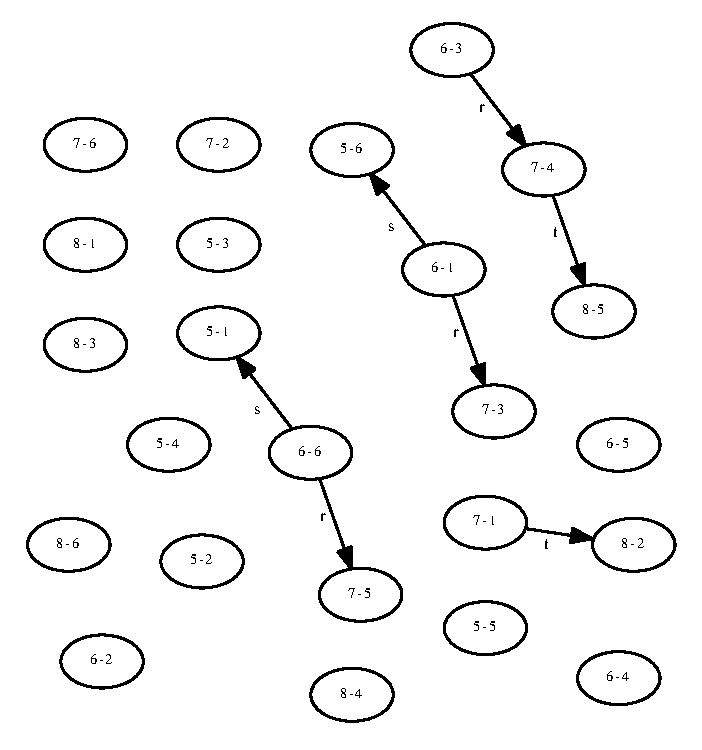
\includegraphics[scale=0.45, bb=0 0 400 410]{python/ex_K_i1-x-g.eps}
\caption{$\cP_1^\prime=\Theta_1^\prime\times \G_{A_2}$}
\label{fig:K_i1-x-g}
\end{center}
\end{figure}


\begin{figure}
\begin{center}
\psfrag{a}{$x_1$}
\psfrag{b}{$x_2$}
\psfrag{c}{$x_3$}
\psfrag{r}{$y_1$}
\psfrag{s}{$y_2$}
\psfrag{t}{$y_3$}
\psfrag{x}{$z_1$}
\psfrag{y}{$z_2$}
\psfrag{z}{$z_3$}
\psfrag{u}{$y_4$}
\psfrag{1}{\hspace{-1pt}\raisebox{-2pt}{\scriptsize $1$}}
\psfrag{2}{\hspace{-1pt}\raisebox{-2pt}{\scriptsize $2$}}
\psfrag{3}{\hspace{-1pt}\raisebox{-2pt}{\scriptsize $3$}}
\psfrag{4}{\hspace{-1pt}\raisebox{-2pt}{\scriptsize $4$}}
\psfrag{5}{\hspace{-1pt}\raisebox{-2pt}{\scriptsize $5$}}
\psfrag{6}{\hspace{-1pt}\raisebox{-2pt}{\scriptsize $6$}}
\psfrag{7}{\hspace{-1pt}\raisebox{-2pt}{\scriptsize $7$}}
\psfrag{8}{\hspace{-1pt}\raisebox{-2pt}{\scriptsize $8$}}
\psfrag{9}{\hspace{-1pt}\raisebox{-2pt}{\scriptsize $9$}}
\psfrag{10}{\hspace{-2pt}\raisebox{-2pt}{\scriptsize $10$}}
\psfrag{11}{\hspace{-2pt}\raisebox{-2pt}{\scriptsize $11$}}
\psfrag{12}{\hspace{-2pt}\raisebox{-2pt}{\scriptsize $12$}}
\psfrag{13}{\hspace{-2pt}\raisebox{-2pt}{\scriptsize $13$}}
\psfrag{14}{\hspace{-2pt}\raisebox{-2pt}{\scriptsize $14$}}
\psfrag{15}{\hspace{-2pt}\raisebox{-2pt}{\scriptsize $15$}}
\psfrag{16}{\hspace{-2pt}\raisebox{-2pt}{\scriptsize $16$}}
\psfrag{17}{\hspace{-2pt}\raisebox{-2pt}{\scriptsize $17$}}
\psfrag{18}{\hspace{-2pt}\raisebox{-2pt}{\scriptsize $18$}}
\psfrag{19}{\hspace{-2pt}\raisebox{-2pt}{\scriptsize $19$}}
\psfrag{20}{\hspace{-2pt}\raisebox{-2pt}{\scriptsize $20$}}
\psfrag{21}{\hspace{-2pt}\raisebox{-2pt}{\scriptsize $21$}}
\psfrag{22}{\hspace{-2pt}\raisebox{-2pt}{\scriptsize $22$}}
\psfrag{23}{\hspace{-2pt}\raisebox{-2pt}{\scriptsize $23$}}
\psfrag{24}{\hspace{-2pt}\raisebox{-2pt}{\scriptsize $24$}}
\psfrag{25}{\hspace{-2pt}\raisebox{-2pt}{\scriptsize $25$}}
\psfrag{26}{\hspace{-2pt}\raisebox{-2pt}{\scriptsize $26$}}
\psfrag{27}{\hspace{-2pt}\raisebox{-2pt}{\scriptsize $27$}}
\psfrag{28}{\hspace{-2pt}\raisebox{-2pt}{\scriptsize $28$}}
\psfrag{29}{\hspace{-2pt}\raisebox{-2pt}{\scriptsize $29$}}
\psfrag{30}{\hspace{-2pt}\raisebox{-2pt}{\scriptsize $30$}}
\psfrag{31}{\hspace{-2pt}\raisebox{-2pt}{\scriptsize $31$}}
\psfrag{32}{\hspace{-2pt}\raisebox{-2pt}{\scriptsize $32$}}
\psfrag{33}{\hspace{-2pt}\raisebox{-2pt}{\scriptsize $33$}}
\psfrag{34}{\hspace{-2pt}\raisebox{-2pt}{\scriptsize $34$}}
\psfrag{35}{\hspace{-2pt}\raisebox{-2pt}{\scriptsize $35$}}
\psfrag{36}{\hspace{-2pt}\raisebox{-2pt}{\scriptsize $36$}}
\psfrag{37}{\hspace{-2pt}\raisebox{-2pt}{\scriptsize $37$}}
\psfrag{38}{\hspace{-2pt}\raisebox{-2pt}{\scriptsize $38$}}
\psfrag{39}{\hspace{-2pt}\raisebox{-2pt}{\scriptsize $39$}}
\psfrag{40}{\hspace{-2pt}\raisebox{-2pt}{\scriptsize $40$}}
\psfrag{41}{\hspace{-2pt}\raisebox{-2pt}{\scriptsize $41$}}
\psfrag{42}{\hspace{-2pt}\raisebox{-2pt}{\scriptsize $42$}}
\psfrag{43}{\hspace{-2pt}\raisebox{-2pt}{\scriptsize $43$}}
\psfrag{44}{\hspace{-2pt}\raisebox{-2pt}{\scriptsize $44$}}
\psfrag{45}{\hspace{-2pt}\raisebox{-2pt}{\scriptsize $45$}}
\psfrag{46}{\hspace{-2pt}\raisebox{-2pt}{\scriptsize $46$}}
\psfrag{47}{\hspace{-2pt}\raisebox{-2pt}{\scriptsize $47$}}
\psfrag{48}{\hspace{-2pt}\raisebox{-2pt}{\scriptsize $48$}}
\psfrag{49}{\hspace{-2pt}\raisebox{-2pt}{\scriptsize $49$}}
\begin{subfigure}[b]{.3\columnwidth}
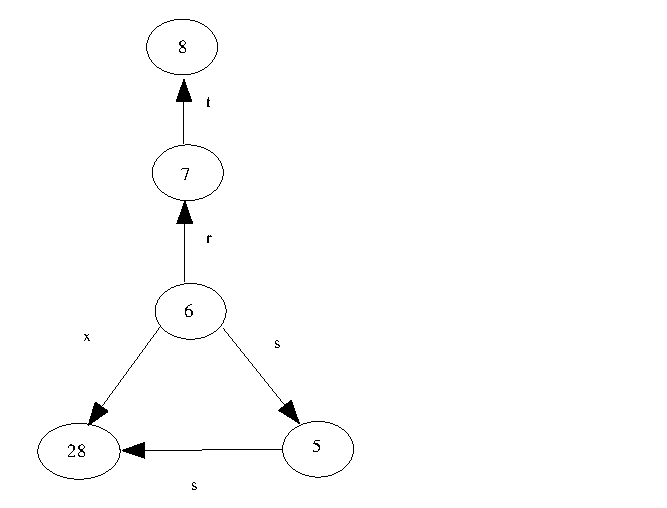
\includegraphics[scale=0.45, bb=0 0  82 280]{python/ex_K_i4.eps}
\caption{$\Theta_5^\prime$}
\label{fig:K_i4}
\end{subfigure}
\hspace*{2cm}
\begin{subfigure}[b]{.3\columnwidth}
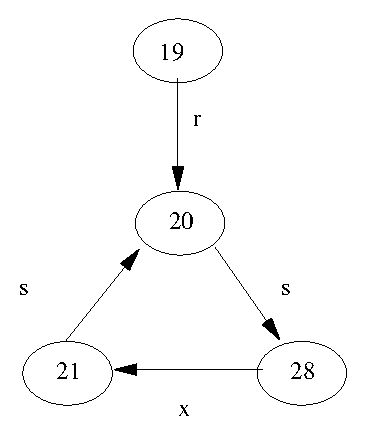
\includegraphics[scale=0.45, bb=0 0 82 210]{python/ex_K_j4.eps}
\caption{$\Theta_5^{\prime\prime}$}
\label{fig:K_j4}
\end{subfigure}
\end{center}
\caption{$X_2$ components}
\label{fig:KY5}
\end{figure}


\begin{figure}
\begin{center}
\psfrag{1-1}{\hspace{-4pt}\raisebox{-2pt}{\scriptsize $1,1$}}
\psfrag{1-2}{\hspace{-4pt}\raisebox{-2pt}{\scriptsize $1,2$}}
\psfrag{1-3}{\hspace{-4pt}\raisebox{-2pt}{\scriptsize $1,3$}}
\psfrag{1-4}{\hspace{-4pt}\raisebox{-2pt}{\scriptsize $1,4$}}
\psfrag{1-5}{\hspace{-4pt}\raisebox{-2pt}{\scriptsize $1,5$}}
\psfrag{1-6}{\hspace{-4pt}\raisebox{-2pt}{\scriptsize $1,6$}}
\psfrag{1-7}{\hspace{-4pt}\raisebox{-2pt}{\scriptsize $1,7$}}
\psfrag{1-8}{\hspace{-4pt}\raisebox{-2pt}{\scriptsize $1,8$}}
\psfrag{1-9}{\hspace{-4pt}\raisebox{-2pt}{\scriptsize $1,9$}}
\psfrag{2-1}{\hspace{-4pt}\raisebox{-2pt}{\scriptsize $2,1$}}
\psfrag{2-2}{\hspace{-4pt}\raisebox{-2pt}{\scriptsize $2,2$}}
\psfrag{2-3}{\hspace{-4pt}\raisebox{-2pt}{\scriptsize $2,3$}}
\psfrag{2-4}{\hspace{-4pt}\raisebox{-2pt}{\scriptsize $2,4$}}
\psfrag{2-5}{\hspace{-4pt}\raisebox{-2pt}{\scriptsize $2,5$}}
\psfrag{2-6}{\hspace{-4pt}\raisebox{-2pt}{\scriptsize $2,6$}}
\psfrag{2-7}{\hspace{-4pt}\raisebox{-2pt}{\scriptsize $2,7$}}
\psfrag{2-8}{\hspace{-4pt}\raisebox{-2pt}{\scriptsize $2,8$}}
\psfrag{2-9}{\hspace{-4pt}\raisebox{-2pt}{\scriptsize $2,9$}}
\psfrag{3-1}{\hspace{-4pt}\raisebox{-2pt}{\scriptsize $3,1$}}
\psfrag{3-2}{\hspace{-4pt}\raisebox{-2pt}{\scriptsize $3,2$}}
\psfrag{3-3}{\hspace{-4pt}\raisebox{-2pt}{\scriptsize $3,3$}}
\psfrag{3-4}{\hspace{-4pt}\raisebox{-2pt}{\scriptsize $3,4$}}
\psfrag{3-5}{\hspace{-4pt}\raisebox{-2pt}{\scriptsize $3,5$}}
\psfrag{3-6}{\hspace{-4pt}\raisebox{-2pt}{\scriptsize $3,6$}}
\psfrag{3-7}{\hspace{-4pt}\raisebox{-2pt}{\scriptsize $3,7$}}
\psfrag{3-8}{\hspace{-4pt}\raisebox{-2pt}{\scriptsize $3,8$}}
\psfrag{3-9}{\hspace{-4pt}\raisebox{-2pt}{\scriptsize $3,9$}}
\psfrag{4-1}{\hspace{-4pt}\raisebox{-2pt}{\scriptsize $4,1$}}
\psfrag{4-2}{\hspace{-4pt}\raisebox{-2pt}{\scriptsize $4,2$}}
\psfrag{4-3}{\hspace{-4pt}\raisebox{-2pt}{\scriptsize $4,3$}}
\psfrag{4-4}{\hspace{-4pt}\raisebox{-2pt}{\scriptsize $4,4$}}
\psfrag{4-5}{\hspace{-4pt}\raisebox{-2pt}{\scriptsize $4,5$}}
\psfrag{4-6}{\hspace{-4pt}\raisebox{-2pt}{\scriptsize $4,6$}}
\psfrag{4-7}{\hspace{-4pt}\raisebox{-2pt}{\scriptsize $4,7$}}
\psfrag{4-8}{\hspace{-4pt}\raisebox{-2pt}{\scriptsize $4,8$}}
\psfrag{4-9}{\hspace{-4pt}\raisebox{-2pt}{\scriptsize $4,9$}}
\psfrag{5-1}{\hspace{-4pt}\raisebox{-2pt}{\scriptsize $5,1$}}
\psfrag{5-2}{\hspace{-4pt}\raisebox{-2pt}{\scriptsize $5,2$}}
\psfrag{5-3}{\hspace{-4pt}\raisebox{-2pt}{\scriptsize $5,3$}}
\psfrag{5-4}{\hspace{-4pt}\raisebox{-2pt}{\scriptsize $5,4$}}
\psfrag{5-5}{\hspace{-4pt}\raisebox{-2pt}{\scriptsize $5,5$}}
\psfrag{5-6}{\hspace{-4pt}\raisebox{-2pt}{\scriptsize $5,6$}}
\psfrag{5-7}{\hspace{-4pt}\raisebox{-2pt}{\scriptsize $5,7$}}
\psfrag{5-8}{\hspace{-4pt}\raisebox{-2pt}{\scriptsize $5,8$}}
\psfrag{5-9}{\hspace{-4pt}\raisebox{-2pt}{\scriptsize $5,9$}}
\psfrag{6-1}{\hspace{-4pt}\raisebox{-2pt}{\scriptsize $6,1$}}
\psfrag{6-2}{\hspace{-4pt}\raisebox{-2pt}{\scriptsize $6,2$}}
\psfrag{6-3}{\hspace{-4pt}\raisebox{-2pt}{\scriptsize $6,3$}}
\psfrag{6-4}{\hspace{-4pt}\raisebox{-2pt}{\scriptsize $6,4$}}
\psfrag{6-5}{\hspace{-4pt}\raisebox{-2pt}{\scriptsize $6,5$}}
\psfrag{6-6}{\hspace{-4pt}\raisebox{-2pt}{\scriptsize $6,6$}}
\psfrag{6-7}{\hspace{-4pt}\raisebox{-2pt}{\scriptsize $6,7$}}
\psfrag{6-8}{\hspace{-4pt}\raisebox{-2pt}{\scriptsize $6,8$}}
\psfrag{6-9}{\hspace{-4pt}\raisebox{-2pt}{\scriptsize $6,9$}}
\psfrag{7-1}{\hspace{-4pt}\raisebox{-2pt}{\scriptsize $7,1$}}
\psfrag{7-2}{\hspace{-4pt}\raisebox{-2pt}{\scriptsize $7,2$}}
\psfrag{7-3}{\hspace{-4pt}\raisebox{-2pt}{\scriptsize $7,3$}}
\psfrag{7-4}{\hspace{-4pt}\raisebox{-2pt}{\scriptsize $7,4$}}
\psfrag{7-5}{\hspace{-4pt}\raisebox{-2pt}{\scriptsize $7,5$}}
\psfrag{7-6}{\hspace{-4pt}\raisebox{-2pt}{\scriptsize $7,6$}}
\psfrag{7-7}{\hspace{-4pt}\raisebox{-2pt}{\scriptsize $7,7$}}
\psfrag{7-8}{\hspace{-4pt}\raisebox{-2pt}{\scriptsize $7,8$}}
\psfrag{7-9}{\hspace{-4pt}\raisebox{-2pt}{\scriptsize $7,9$}}
\psfrag{8-1}{\hspace{-4pt}\raisebox{-2pt}{\scriptsize $8,1$}}
\psfrag{8-2}{\hspace{-4pt}\raisebox{-2pt}{\scriptsize $8,2$}}
\psfrag{8-3}{\hspace{-4pt}\raisebox{-2pt}{\scriptsize $8,3$}}
\psfrag{8-4}{\hspace{-4pt}\raisebox{-2pt}{\scriptsize $8,4$}}
\psfrag{8-5}{\hspace{-4pt}\raisebox{-2pt}{\scriptsize $8,5$}}
\psfrag{8-6}{\hspace{-4pt}\raisebox{-2pt}{\scriptsize $8,6$}}
\psfrag{8-7}{\hspace{-4pt}\raisebox{-2pt}{\scriptsize $8,7$}}
\psfrag{8-8}{\hspace{-4pt}\raisebox{-2pt}{\scriptsize $8,8$}}
\psfrag{8-9}{\hspace{-4pt}\raisebox{-2pt}{\scriptsize $8,9$}}
\psfrag{9-1}{\hspace{-4pt}\raisebox{-2pt}{\scriptsize $9,1$}}
\psfrag{9-2}{\hspace{-4pt}\raisebox{-2pt}{\scriptsize $9,2$}}
\psfrag{9-3}{\hspace{-4pt}\raisebox{-2pt}{\scriptsize $9,3$}}
\psfrag{9-4}{\hspace{-4pt}\raisebox{-2pt}{\scriptsize $9,4$}}
\psfrag{9-5}{\hspace{-4pt}\raisebox{-2pt}{\scriptsize $9,5$}}
\psfrag{9-6}{\hspace{-4pt}\raisebox{-2pt}{\scriptsize $9,6$}}
\psfrag{9-7}{\hspace{-4pt}\raisebox{-2pt}{\scriptsize $9,7$}}
\psfrag{9-8}{\hspace{-4pt}\raisebox{-2pt}{\scriptsize $9,8$}}
\psfrag{9-9}{\hspace{-4pt}\raisebox{-2pt}{\scriptsize $9,9$}}
\psfrag{10-1}{\hspace{-4pt}\raisebox{-2pt}{\scriptsize $10,1$}}
\psfrag{10-2}{\hspace{-4pt}\raisebox{-2pt}{\scriptsize $10,2$}}
\psfrag{10-3}{\hspace{-4pt}\raisebox{-2pt}{\scriptsize $10,3$}}
\psfrag{10-4}{\hspace{-4pt}\raisebox{-2pt}{\scriptsize $10,4$}}
\psfrag{10-5}{\hspace{-4pt}\raisebox{-2pt}{\scriptsize $10,5$}}
\psfrag{10-6}{\hspace{-4pt}\raisebox{-2pt}{\scriptsize $10,6$}}
\psfrag{10-7}{\hspace{-4pt}\raisebox{-2pt}{\scriptsize $10,7$}}
\psfrag{10-8}{\hspace{-4pt}\raisebox{-2pt}{\scriptsize $10,8$}}
\psfrag{10-9}{\hspace{-4pt}\raisebox{-2pt}{\scriptsize $10,9$}}
\psfrag{11-1}{\hspace{-4pt}\raisebox{-2pt}{\scriptsize $11,1$}}
\psfrag{11-2}{\hspace{-4pt}\raisebox{-2pt}{\scriptsize $11,2$}}
\psfrag{11-3}{\hspace{-4pt}\raisebox{-2pt}{\scriptsize $11,3$}}
\psfrag{11-4}{\hspace{-4pt}\raisebox{-2pt}{\scriptsize $11,4$}}
\psfrag{11-5}{\hspace{-4pt}\raisebox{-2pt}{\scriptsize $11,5$}}
\psfrag{11-6}{\hspace{-4pt}\raisebox{-2pt}{\scriptsize $11,6$}}
\psfrag{11-7}{\hspace{-4pt}\raisebox{-2pt}{\scriptsize $11,7$}}
\psfrag{11-8}{\hspace{-4pt}\raisebox{-2pt}{\scriptsize $11,8$}}
\psfrag{11-9}{\hspace{-4pt}\raisebox{-2pt}{\scriptsize $11,9$}}
\psfrag{12-1}{\hspace{-4pt}\raisebox{-2pt}{\scriptsize $12,1$}}
\psfrag{12-2}{\hspace{-4pt}\raisebox{-2pt}{\scriptsize $12,2$}}
\psfrag{12-3}{\hspace{-4pt}\raisebox{-2pt}{\scriptsize $12,3$}}
\psfrag{12-4}{\hspace{-4pt}\raisebox{-2pt}{\scriptsize $12,4$}}
\psfrag{12-5}{\hspace{-4pt}\raisebox{-2pt}{\scriptsize $12,5$}}
\psfrag{12-6}{\hspace{-4pt}\raisebox{-2pt}{\scriptsize $12,6$}}
\psfrag{12-7}{\hspace{-4pt}\raisebox{-2pt}{\scriptsize $12,7$}}
\psfrag{12-8}{\hspace{-4pt}\raisebox{-2pt}{\scriptsize $12,8$}}
\psfrag{12-9}{\hspace{-4pt}\raisebox{-2pt}{\scriptsize $12,9$}}
\psfrag{13-1}{\hspace{-4pt}\raisebox{-2pt}{\scriptsize $13,1$}}
\psfrag{13-2}{\hspace{-4pt}\raisebox{-2pt}{\scriptsize $13,2$}}
\psfrag{13-3}{\hspace{-4pt}\raisebox{-2pt}{\scriptsize $13,3$}}
\psfrag{13-4}{\hspace{-4pt}\raisebox{-2pt}{\scriptsize $13,4$}}
\psfrag{13-5}{\hspace{-4pt}\raisebox{-2pt}{\scriptsize $13,5$}}
\psfrag{13-6}{\hspace{-4pt}\raisebox{-2pt}{\scriptsize $13,6$}}
\psfrag{13-7}{\hspace{-4pt}\raisebox{-2pt}{\scriptsize $13,7$}}
\psfrag{13-8}{\hspace{-4pt}\raisebox{-2pt}{\scriptsize $13,8$}}
\psfrag{13-9}{\hspace{-4pt}\raisebox{-2pt}{\scriptsize $13,9$}}
\psfrag{14-1}{\hspace{-4pt}\raisebox{-2pt}{\scriptsize $14,1$}}
\psfrag{14-2}{\hspace{-4pt}\raisebox{-2pt}{\scriptsize $14,2$}}
\psfrag{14-3}{\hspace{-4pt}\raisebox{-2pt}{\scriptsize $14,3$}}
\psfrag{14-4}{\hspace{-4pt}\raisebox{-2pt}{\scriptsize $14,4$}}
\psfrag{14-5}{\hspace{-4pt}\raisebox{-2pt}{\scriptsize $14,5$}}
\psfrag{14-6}{\hspace{-4pt}\raisebox{-2pt}{\scriptsize $14,6$}}
\psfrag{14-7}{\hspace{-4pt}\raisebox{-2pt}{\scriptsize $14,7$}}
\psfrag{14-8}{\hspace{-4pt}\raisebox{-2pt}{\scriptsize $14,8$}}
\psfrag{14-9}{\hspace{-4pt}\raisebox{-2pt}{\scriptsize $14,9$}}
\psfrag{15-1}{\hspace{-4pt}\raisebox{-2pt}{\scriptsize $15,1$}}
\psfrag{15-2}{\hspace{-4pt}\raisebox{-2pt}{\scriptsize $15,2$}}
\psfrag{15-3}{\hspace{-4pt}\raisebox{-2pt}{\scriptsize $15,3$}}
\psfrag{15-4}{\hspace{-4pt}\raisebox{-2pt}{\scriptsize $15,4$}}
\psfrag{15-5}{\hspace{-4pt}\raisebox{-2pt}{\scriptsize $15,5$}}
\psfrag{15-6}{\hspace{-4pt}\raisebox{-2pt}{\scriptsize $15,6$}}
\psfrag{15-7}{\hspace{-4pt}\raisebox{-2pt}{\scriptsize $15,7$}}
\psfrag{15-8}{\hspace{-4pt}\raisebox{-2pt}{\scriptsize $15,8$}}
\psfrag{15-9}{\hspace{-4pt}\raisebox{-2pt}{\scriptsize $15,9$}}
\psfrag{16-1}{\hspace{-4pt}\raisebox{-2pt}{\scriptsize $16,1$}}
\psfrag{16-2}{\hspace{-4pt}\raisebox{-2pt}{\scriptsize $16,2$}}
\psfrag{16-3}{\hspace{-4pt}\raisebox{-2pt}{\scriptsize $16,3$}}
\psfrag{16-4}{\hspace{-4pt}\raisebox{-2pt}{\scriptsize $16,4$}}
\psfrag{16-5}{\hspace{-4pt}\raisebox{-2pt}{\scriptsize $16,5$}}
\psfrag{16-6}{\hspace{-4pt}\raisebox{-2pt}{\scriptsize $16,6$}}
\psfrag{16-7}{\hspace{-4pt}\raisebox{-2pt}{\scriptsize $16,7$}}
\psfrag{16-8}{\hspace{-4pt}\raisebox{-2pt}{\scriptsize $16,8$}}
\psfrag{16-9}{\hspace{-4pt}\raisebox{-2pt}{\scriptsize $16,9$}}
\psfrag{17-1}{\hspace{-4pt}\raisebox{-2pt}{\scriptsize $17,1$}}
\psfrag{17-2}{\hspace{-4pt}\raisebox{-2pt}{\scriptsize $17,2$}}
\psfrag{17-3}{\hspace{-4pt}\raisebox{-2pt}{\scriptsize $17,3$}}
\psfrag{17-4}{\hspace{-4pt}\raisebox{-2pt}{\scriptsize $17,4$}}
\psfrag{17-5}{\hspace{-4pt}\raisebox{-2pt}{\scriptsize $17,5$}}
\psfrag{17-6}{\hspace{-4pt}\raisebox{-2pt}{\scriptsize $17,6$}}
\psfrag{17-7}{\hspace{-4pt}\raisebox{-2pt}{\scriptsize $17,7$}}
\psfrag{17-8}{\hspace{-4pt}\raisebox{-2pt}{\scriptsize $17,8$}}
\psfrag{17-9}{\hspace{-4pt}\raisebox{-2pt}{\scriptsize $17,9$}}
\psfrag{18-1}{\hspace{-4pt}\raisebox{-2pt}{\scriptsize $18,1$}}
\psfrag{18-2}{\hspace{-4pt}\raisebox{-2pt}{\scriptsize $18,2$}}
\psfrag{18-3}{\hspace{-4pt}\raisebox{-2pt}{\scriptsize $18,3$}}
\psfrag{18-4}{\hspace{-4pt}\raisebox{-2pt}{\scriptsize $18,4$}}
\psfrag{18-5}{\hspace{-4pt}\raisebox{-2pt}{\scriptsize $18,5$}}
\psfrag{18-6}{\hspace{-4pt}\raisebox{-2pt}{\scriptsize $18,6$}}
\psfrag{18-7}{\hspace{-4pt}\raisebox{-2pt}{\scriptsize $18,7$}}
\psfrag{18-8}{\hspace{-4pt}\raisebox{-2pt}{\scriptsize $18,8$}}
\psfrag{18-9}{\hspace{-4pt}\raisebox{-2pt}{\scriptsize $18,9$}}
\psfrag{19-1}{\hspace{-4pt}\raisebox{-2pt}{\scriptsize $19,1$}}
\psfrag{19-2}{\hspace{-4pt}\raisebox{-2pt}{\scriptsize $19,2$}}
\psfrag{19-3}{\hspace{-4pt}\raisebox{-2pt}{\scriptsize $19,3$}}
\psfrag{19-4}{\hspace{-4pt}\raisebox{-2pt}{\scriptsize $19,4$}}
\psfrag{19-5}{\hspace{-4pt}\raisebox{-2pt}{\scriptsize $19,5$}}
\psfrag{19-6}{\hspace{-4pt}\raisebox{-2pt}{\scriptsize $19,6$}}
\psfrag{19-7}{\hspace{-4pt}\raisebox{-2pt}{\scriptsize $19,7$}}
\psfrag{19-8}{\hspace{-4pt}\raisebox{-2pt}{\scriptsize $19,8$}}
\psfrag{19-9}{\hspace{-4pt}\raisebox{-2pt}{\scriptsize $19,9$}}
\psfrag{20-1}{\hspace{-4pt}\raisebox{-2pt}{\scriptsize $20,1$}}
\psfrag{20-2}{\hspace{-4pt}\raisebox{-2pt}{\scriptsize $20,2$}}
\psfrag{20-3}{\hspace{-4pt}\raisebox{-2pt}{\scriptsize $20,3$}}
\psfrag{20-4}{\hspace{-4pt}\raisebox{-2pt}{\scriptsize $20,4$}}
\psfrag{20-5}{\hspace{-4pt}\raisebox{-2pt}{\scriptsize $20,5$}}
\psfrag{20-6}{\hspace{-4pt}\raisebox{-2pt}{\scriptsize $20,6$}}
\psfrag{20-7}{\hspace{-4pt}\raisebox{-2pt}{\scriptsize $20,7$}}
\psfrag{20-8}{\hspace{-4pt}\raisebox{-2pt}{\scriptsize $20,8$}}
\psfrag{20-9}{\hspace{-4pt}\raisebox{-2pt}{\scriptsize $20,9$}}
\psfrag{21-1}{\hspace{-4pt}\raisebox{-2pt}{\scriptsize $21,1$}}
\psfrag{21-2}{\hspace{-4pt}\raisebox{-2pt}{\scriptsize $21,2$}}
\psfrag{21-3}{\hspace{-4pt}\raisebox{-2pt}{\scriptsize $21,3$}}
\psfrag{21-4}{\hspace{-4pt}\raisebox{-2pt}{\scriptsize $21,4$}}
\psfrag{21-5}{\hspace{-4pt}\raisebox{-2pt}{\scriptsize $21,5$}}
\psfrag{21-6}{\hspace{-4pt}\raisebox{-2pt}{\scriptsize $21,6$}}
\psfrag{21-7}{\hspace{-4pt}\raisebox{-2pt}{\scriptsize $21,7$}}
\psfrag{21-8}{\hspace{-4pt}\raisebox{-2pt}{\scriptsize $21,8$}}
\psfrag{21-9}{\hspace{-4pt}\raisebox{-2pt}{\scriptsize $21,9$}}
\psfrag{22-1}{\hspace{-4pt}\raisebox{-2pt}{\scriptsize $22,1$}}
\psfrag{22-2}{\hspace{-4pt}\raisebox{-2pt}{\scriptsize $22,2$}}
\psfrag{22-3}{\hspace{-4pt}\raisebox{-2pt}{\scriptsize $22,3$}}
\psfrag{22-4}{\hspace{-4pt}\raisebox{-2pt}{\scriptsize $22,4$}}
\psfrag{22-5}{\hspace{-4pt}\raisebox{-2pt}{\scriptsize $22,5$}}
\psfrag{22-6}{\hspace{-4pt}\raisebox{-2pt}{\scriptsize $22,6$}}
\psfrag{22-7}{\hspace{-4pt}\raisebox{-2pt}{\scriptsize $22,7$}}
\psfrag{22-8}{\hspace{-4pt}\raisebox{-2pt}{\scriptsize $22,8$}}
\psfrag{22-9}{\hspace{-4pt}\raisebox{-2pt}{\scriptsize $22,9$}}
\psfrag{23-1}{\hspace{-4pt}\raisebox{-2pt}{\scriptsize $23,1$}}
\psfrag{23-2}{\hspace{-4pt}\raisebox{-2pt}{\scriptsize $23,2$}}
\psfrag{23-3}{\hspace{-4pt}\raisebox{-2pt}{\scriptsize $23,3$}}
\psfrag{23-4}{\hspace{-4pt}\raisebox{-2pt}{\scriptsize $23,4$}}
\psfrag{23-5}{\hspace{-4pt}\raisebox{-2pt}{\scriptsize $23,5$}}
\psfrag{23-6}{\hspace{-4pt}\raisebox{-2pt}{\scriptsize $23,6$}}
\psfrag{23-7}{\hspace{-4pt}\raisebox{-2pt}{\scriptsize $23,7$}}
\psfrag{23-8}{\hspace{-4pt}\raisebox{-2pt}{\scriptsize $23,8$}}
\psfrag{23-9}{\hspace{-4pt}\raisebox{-2pt}{\scriptsize $23,9$}}
\psfrag{24-1}{\hspace{-4pt}\raisebox{-2pt}{\scriptsize $24,1$}}
\psfrag{24-2}{\hspace{-4pt}\raisebox{-2pt}{\scriptsize $24,2$}}
\psfrag{24-3}{\hspace{-4pt}\raisebox{-2pt}{\scriptsize $24,3$}}
\psfrag{24-4}{\hspace{-4pt}\raisebox{-2pt}{\scriptsize $24,4$}}
\psfrag{24-5}{\hspace{-4pt}\raisebox{-2pt}{\scriptsize $24,5$}}
\psfrag{24-6}{\hspace{-4pt}\raisebox{-2pt}{\scriptsize $24,6$}}
\psfrag{24-7}{\hspace{-4pt}\raisebox{-2pt}{\scriptsize $24,7$}}
\psfrag{24-8}{\hspace{-4pt}\raisebox{-2pt}{\scriptsize $24,8$}}
\psfrag{24-9}{\hspace{-4pt}\raisebox{-2pt}{\scriptsize $24,9$}}
\psfrag{25-1}{\hspace{-4pt}\raisebox{-2pt}{\scriptsize $25,1$}}
\psfrag{25-2}{\hspace{-4pt}\raisebox{-2pt}{\scriptsize $25,2$}}
\psfrag{25-3}{\hspace{-4pt}\raisebox{-2pt}{\scriptsize $25,3$}}
\psfrag{25-4}{\hspace{-4pt}\raisebox{-2pt}{\scriptsize $25,4$}}
\psfrag{25-5}{\hspace{-4pt}\raisebox{-2pt}{\scriptsize $25,5$}}
\psfrag{25-6}{\hspace{-4pt}\raisebox{-2pt}{\scriptsize $25,6$}}
\psfrag{25-7}{\hspace{-4pt}\raisebox{-2pt}{\scriptsize $25,7$}}
\psfrag{25-8}{\hspace{-4pt}\raisebox{-2pt}{\scriptsize $25,8$}}
\psfrag{25-9}{\hspace{-4pt}\raisebox{-2pt}{\scriptsize $25,9$}}
\psfrag{26-1}{\hspace{-4pt}\raisebox{-2pt}{\scriptsize $26,1$}}
\psfrag{26-2}{\hspace{-4pt}\raisebox{-2pt}{\scriptsize $26,2$}}
\psfrag{26-3}{\hspace{-4pt}\raisebox{-2pt}{\scriptsize $26,3$}}
\psfrag{26-4}{\hspace{-4pt}\raisebox{-2pt}{\scriptsize $26,4$}}
\psfrag{26-5}{\hspace{-4pt}\raisebox{-2pt}{\scriptsize $26,5$}}
\psfrag{26-6}{\hspace{-4pt}\raisebox{-2pt}{\scriptsize $26,6$}}
\psfrag{26-7}{\hspace{-4pt}\raisebox{-2pt}{\scriptsize $26,7$}}
\psfrag{26-8}{\hspace{-4pt}\raisebox{-2pt}{\scriptsize $26,8$}}
\psfrag{26-9}{\hspace{-4pt}\raisebox{-2pt}{\scriptsize $26,9$}}
\psfrag{27-1}{\hspace{-4pt}\raisebox{-2pt}{\scriptsize $27,1$}}
\psfrag{27-2}{\hspace{-4pt}\raisebox{-2pt}{\scriptsize $27,2$}}
\psfrag{27-3}{\hspace{-4pt}\raisebox{-2pt}{\scriptsize $27,3$}}
\psfrag{27-4}{\hspace{-4pt}\raisebox{-2pt}{\scriptsize $27,4$}}
\psfrag{27-5}{\hspace{-4pt}\raisebox{-2pt}{\scriptsize $27,5$}}
\psfrag{27-6}{\hspace{-4pt}\raisebox{-2pt}{\scriptsize $27,6$}}
\psfrag{27-7}{\hspace{-4pt}\raisebox{-2pt}{\scriptsize $27,7$}}
\psfrag{27-8}{\hspace{-4pt}\raisebox{-2pt}{\scriptsize $27,8$}}
\psfrag{27-9}{\hspace{-4pt}\raisebox{-2pt}{\scriptsize $27,9$}}
\psfrag{28-1}{\hspace{-4pt}\raisebox{-2pt}{\scriptsize $28,1$}}
\psfrag{28-2}{\hspace{-4pt}\raisebox{-2pt}{\scriptsize $28,2$}}
\psfrag{28-3}{\hspace{-4pt}\raisebox{-2pt}{\scriptsize $28,3$}}
\psfrag{28-4}{\hspace{-4pt}\raisebox{-2pt}{\scriptsize $28,4$}}
\psfrag{28-5}{\hspace{-4pt}\raisebox{-2pt}{\scriptsize $28,5$}}
\psfrag{28-6}{\hspace{-4pt}\raisebox{-2pt}{\scriptsize $28,6$}}
\psfrag{28-7}{\hspace{-4pt}\raisebox{-2pt}{\scriptsize $28,7$}}
\psfrag{28-8}{\hspace{-4pt}\raisebox{-2pt}{\scriptsize $28,8$}}
\psfrag{28-9}{\hspace{-4pt}\raisebox{-2pt}{\scriptsize $28,9$}}
\psfrag{29-1}{\hspace{-4pt}\raisebox{-2pt}{\scriptsize $29,1$}}
\psfrag{29-2}{\hspace{-4pt}\raisebox{-2pt}{\scriptsize $29,2$}}
\psfrag{29-3}{\hspace{-4pt}\raisebox{-2pt}{\scriptsize $29,3$}}
\psfrag{29-4}{\hspace{-4pt}\raisebox{-2pt}{\scriptsize $29,4$}}
\psfrag{29-5}{\hspace{-4pt}\raisebox{-2pt}{\scriptsize $29,5$}}
\psfrag{29-6}{\hspace{-4pt}\raisebox{-2pt}{\scriptsize $29,6$}}
\psfrag{29-7}{\hspace{-4pt}\raisebox{-2pt}{\scriptsize $29,7$}}
\psfrag{29-8}{\hspace{-4pt}\raisebox{-2pt}{\scriptsize $29,8$}}
\psfrag{29-9}{\hspace{-4pt}\raisebox{-2pt}{\scriptsize $29,9$}}
\psfrag{30-1}{\hspace{-4pt}\raisebox{-2pt}{\scriptsize $30,1$}}
\psfrag{30-2}{\hspace{-4pt}\raisebox{-2pt}{\scriptsize $30,2$}}
\psfrag{30-3}{\hspace{-4pt}\raisebox{-2pt}{\scriptsize $30,3$}}
\psfrag{30-4}{\hspace{-4pt}\raisebox{-2pt}{\scriptsize $30,4$}}
\psfrag{30-5}{\hspace{-4pt}\raisebox{-2pt}{\scriptsize $30,5$}}
\psfrag{30-6}{\hspace{-4pt}\raisebox{-2pt}{\scriptsize $30,6$}}
\psfrag{30-7}{\hspace{-4pt}\raisebox{-2pt}{\scriptsize $30,7$}}
\psfrag{30-8}{\hspace{-4pt}\raisebox{-2pt}{\scriptsize $30,8$}}
\psfrag{30-9}{\hspace{-4pt}\raisebox{-2pt}{\scriptsize $30,9$}}
\psfrag{31-1}{\hspace{-4pt}\raisebox{-2pt}{\scriptsize $31,1$}}
\psfrag{31-2}{\hspace{-4pt}\raisebox{-2pt}{\scriptsize $31,2$}}
\psfrag{31-3}{\hspace{-4pt}\raisebox{-2pt}{\scriptsize $31,3$}}
\psfrag{31-4}{\hspace{-4pt}\raisebox{-2pt}{\scriptsize $31,4$}}
\psfrag{31-5}{\hspace{-4pt}\raisebox{-2pt}{\scriptsize $31,5$}}
\psfrag{31-6}{\hspace{-4pt}\raisebox{-2pt}{\scriptsize $31,6$}}
\psfrag{31-7}{\hspace{-4pt}\raisebox{-2pt}{\scriptsize $31,7$}}
\psfrag{31-8}{\hspace{-4pt}\raisebox{-2pt}{\scriptsize $31,8$}}
\psfrag{31-9}{\hspace{-4pt}\raisebox{-2pt}{\scriptsize $31,9$}}
\psfrag{32-1}{\hspace{-4pt}\raisebox{-2pt}{\scriptsize $32,1$}}
\psfrag{32-2}{\hspace{-4pt}\raisebox{-2pt}{\scriptsize $32,2$}}
\psfrag{32-3}{\hspace{-4pt}\raisebox{-2pt}{\scriptsize $32,3$}}
\psfrag{32-4}{\hspace{-4pt}\raisebox{-2pt}{\scriptsize $32,4$}}
\psfrag{32-5}{\hspace{-4pt}\raisebox{-2pt}{\scriptsize $32,5$}}
\psfrag{32-6}{\hspace{-4pt}\raisebox{-2pt}{\scriptsize $32,6$}}
\psfrag{32-7}{\hspace{-4pt}\raisebox{-2pt}{\scriptsize $32,7$}}
\psfrag{32-8}{\hspace{-4pt}\raisebox{-2pt}{\scriptsize $32,8$}}
\psfrag{32-9}{\hspace{-4pt}\raisebox{-2pt}{\scriptsize $32,9$}}
\psfrag{33-1}{\hspace{-4pt}\raisebox{-2pt}{\scriptsize $33,1$}}
\psfrag{33-2}{\hspace{-4pt}\raisebox{-2pt}{\scriptsize $33,2$}}
\psfrag{33-3}{\hspace{-4pt}\raisebox{-2pt}{\scriptsize $33,3$}}
\psfrag{33-4}{\hspace{-4pt}\raisebox{-2pt}{\scriptsize $33,4$}}
\psfrag{33-5}{\hspace{-4pt}\raisebox{-2pt}{\scriptsize $33,5$}}
\psfrag{33-6}{\hspace{-4pt}\raisebox{-2pt}{\scriptsize $33,6$}}
\psfrag{33-7}{\hspace{-4pt}\raisebox{-2pt}{\scriptsize $33,7$}}
\psfrag{33-8}{\hspace{-4pt}\raisebox{-2pt}{\scriptsize $33,8$}}
\psfrag{33-9}{\hspace{-4pt}\raisebox{-2pt}{\scriptsize $33,9$}}
\psfrag{34-1}{\hspace{-4pt}\raisebox{-2pt}{\scriptsize $34,1$}}
\psfrag{34-2}{\hspace{-4pt}\raisebox{-2pt}{\scriptsize $34,2$}}
\psfrag{34-3}{\hspace{-4pt}\raisebox{-2pt}{\scriptsize $34,3$}}
\psfrag{34-4}{\hspace{-4pt}\raisebox{-2pt}{\scriptsize $34,4$}}
\psfrag{34-5}{\hspace{-4pt}\raisebox{-2pt}{\scriptsize $34,5$}}
\psfrag{34-6}{\hspace{-4pt}\raisebox{-2pt}{\scriptsize $34,6$}}
\psfrag{34-7}{\hspace{-4pt}\raisebox{-2pt}{\scriptsize $34,7$}}
\psfrag{34-8}{\hspace{-4pt}\raisebox{-2pt}{\scriptsize $34,8$}}
\psfrag{34-9}{\hspace{-4pt}\raisebox{-2pt}{\scriptsize $34,9$}}
\psfrag{35-1}{\hspace{-4pt}\raisebox{-2pt}{\scriptsize $35,1$}}
\psfrag{35-2}{\hspace{-4pt}\raisebox{-2pt}{\scriptsize $35,2$}}
\psfrag{35-3}{\hspace{-4pt}\raisebox{-2pt}{\scriptsize $35,3$}}
\psfrag{35-4}{\hspace{-4pt}\raisebox{-2pt}{\scriptsize $35,4$}}
\psfrag{35-5}{\hspace{-4pt}\raisebox{-2pt}{\scriptsize $35,5$}}
\psfrag{35-6}{\hspace{-4pt}\raisebox{-2pt}{\scriptsize $35,6$}}
\psfrag{35-7}{\hspace{-4pt}\raisebox{-2pt}{\scriptsize $35,7$}}
\psfrag{35-8}{\hspace{-4pt}\raisebox{-2pt}{\scriptsize $35,8$}}
\psfrag{35-9}{\hspace{-4pt}\raisebox{-2pt}{\scriptsize $35,9$}}
\psfrag{36-1}{\hspace{-4pt}\raisebox{-2pt}{\scriptsize $36,1$}}
\psfrag{36-2}{\hspace{-4pt}\raisebox{-2pt}{\scriptsize $36,2$}}
\psfrag{36-3}{\hspace{-4pt}\raisebox{-2pt}{\scriptsize $36,3$}}
\psfrag{36-4}{\hspace{-4pt}\raisebox{-2pt}{\scriptsize $36,4$}}
\psfrag{36-5}{\hspace{-4pt}\raisebox{-2pt}{\scriptsize $36,5$}}
\psfrag{36-6}{\hspace{-4pt}\raisebox{-2pt}{\scriptsize $36,6$}}
\psfrag{36-7}{\hspace{-4pt}\raisebox{-2pt}{\scriptsize $36,7$}}
\psfrag{36-8}{\hspace{-4pt}\raisebox{-2pt}{\scriptsize $36,8$}}
\psfrag{36-9}{\hspace{-4pt}\raisebox{-2pt}{\scriptsize $36,9$}}
\psfrag{37-1}{\hspace{-4pt}\raisebox{-2pt}{\scriptsize $37,1$}}
\psfrag{37-2}{\hspace{-4pt}\raisebox{-2pt}{\scriptsize $37,2$}}
\psfrag{37-3}{\hspace{-4pt}\raisebox{-2pt}{\scriptsize $37,3$}}
\psfrag{37-4}{\hspace{-4pt}\raisebox{-2pt}{\scriptsize $37,4$}}
\psfrag{37-5}{\hspace{-4pt}\raisebox{-2pt}{\scriptsize $37,5$}}
\psfrag{37-6}{\hspace{-4pt}\raisebox{-2pt}{\scriptsize $37,6$}}
\psfrag{37-7}{\hspace{-4pt}\raisebox{-2pt}{\scriptsize $37,7$}}
\psfrag{37-8}{\hspace{-4pt}\raisebox{-2pt}{\scriptsize $37,8$}}
\psfrag{37-9}{\hspace{-4pt}\raisebox{-2pt}{\scriptsize $37,9$}}
\psfrag{38-1}{\hspace{-4pt}\raisebox{-2pt}{\scriptsize $38,1$}}
\psfrag{38-2}{\hspace{-4pt}\raisebox{-2pt}{\scriptsize $38,2$}}
\psfrag{38-3}{\hspace{-4pt}\raisebox{-2pt}{\scriptsize $38,3$}}
\psfrag{38-4}{\hspace{-4pt}\raisebox{-2pt}{\scriptsize $38,4$}}
\psfrag{38-5}{\hspace{-4pt}\raisebox{-2pt}{\scriptsize $38,5$}}
\psfrag{38-6}{\hspace{-4pt}\raisebox{-2pt}{\scriptsize $38,6$}}
\psfrag{38-7}{\hspace{-4pt}\raisebox{-2pt}{\scriptsize $38,7$}}
\psfrag{38-8}{\hspace{-4pt}\raisebox{-2pt}{\scriptsize $38,8$}}
\psfrag{38-9}{\hspace{-4pt}\raisebox{-2pt}{\scriptsize $38,9$}}
\psfrag{39-1}{\hspace{-4pt}\raisebox{-2pt}{\scriptsize $39,1$}}
\psfrag{39-2}{\hspace{-4pt}\raisebox{-2pt}{\scriptsize $39,2$}}
\psfrag{39-3}{\hspace{-4pt}\raisebox{-2pt}{\scriptsize $39,3$}}
\psfrag{39-4}{\hspace{-4pt}\raisebox{-2pt}{\scriptsize $39,4$}}
\psfrag{39-5}{\hspace{-4pt}\raisebox{-2pt}{\scriptsize $39,5$}}
\psfrag{39-6}{\hspace{-4pt}\raisebox{-2pt}{\scriptsize $39,6$}}
\psfrag{39-7}{\hspace{-4pt}\raisebox{-2pt}{\scriptsize $39,7$}}
\psfrag{39-8}{\hspace{-4pt}\raisebox{-2pt}{\scriptsize $39,8$}}
\psfrag{39-9}{\hspace{-4pt}\raisebox{-2pt}{\scriptsize $39,9$}}
\psfrag{40-1}{\hspace{-4pt}\raisebox{-2pt}{\scriptsize $40,1$}}
\psfrag{40-2}{\hspace{-4pt}\raisebox{-2pt}{\scriptsize $40,2$}}
\psfrag{40-3}{\hspace{-4pt}\raisebox{-2pt}{\scriptsize $40,3$}}
\psfrag{40-4}{\hspace{-4pt}\raisebox{-2pt}{\scriptsize $40,4$}}
\psfrag{40-5}{\hspace{-4pt}\raisebox{-2pt}{\scriptsize $40,5$}}
\psfrag{40-6}{\hspace{-4pt}\raisebox{-2pt}{\scriptsize $40,6$}}
\psfrag{40-7}{\hspace{-4pt}\raisebox{-2pt}{\scriptsize $40,7$}}
\psfrag{40-8}{\hspace{-4pt}\raisebox{-2pt}{\scriptsize $40,8$}}
\psfrag{40-9}{\hspace{-4pt}\raisebox{-2pt}{\scriptsize $40,9$}}
\psfrag{41-1}{\hspace{-4pt}\raisebox{-2pt}{\scriptsize $41,1$}}
\psfrag{41-2}{\hspace{-4pt}\raisebox{-2pt}{\scriptsize $41,2$}}
\psfrag{41-3}{\hspace{-4pt}\raisebox{-2pt}{\scriptsize $41,3$}}
\psfrag{41-4}{\hspace{-4pt}\raisebox{-2pt}{\scriptsize $41,4$}}
\psfrag{41-5}{\hspace{-4pt}\raisebox{-2pt}{\scriptsize $41,5$}}
\psfrag{41-6}{\hspace{-4pt}\raisebox{-2pt}{\scriptsize $41,6$}}
\psfrag{41-7}{\hspace{-4pt}\raisebox{-2pt}{\scriptsize $41,7$}}
\psfrag{41-8}{\hspace{-4pt}\raisebox{-2pt}{\scriptsize $41,8$}}
\psfrag{41-9}{\hspace{-4pt}\raisebox{-2pt}{\scriptsize $41,9$}}
\psfrag{42-1}{\hspace{-4pt}\raisebox{-2pt}{\scriptsize $42,1$}}
\psfrag{42-2}{\hspace{-4pt}\raisebox{-2pt}{\scriptsize $42,2$}}
\psfrag{42-3}{\hspace{-4pt}\raisebox{-2pt}{\scriptsize $42,3$}}
\psfrag{42-4}{\hspace{-4pt}\raisebox{-2pt}{\scriptsize $42,4$}}
\psfrag{42-5}{\hspace{-4pt}\raisebox{-2pt}{\scriptsize $42,5$}}
\psfrag{42-6}{\hspace{-4pt}\raisebox{-2pt}{\scriptsize $42,6$}}
\psfrag{42-7}{\hspace{-4pt}\raisebox{-2pt}{\scriptsize $42,7$}}
\psfrag{42-8}{\hspace{-4pt}\raisebox{-2pt}{\scriptsize $42,8$}}
\psfrag{42-9}{\hspace{-4pt}\raisebox{-2pt}{\scriptsize $42,9$}}
\psfrag{43-1}{\hspace{-4pt}\raisebox{-2pt}{\scriptsize $43,1$}}
\psfrag{43-2}{\hspace{-4pt}\raisebox{-2pt}{\scriptsize $43,2$}}
\psfrag{43-3}{\hspace{-4pt}\raisebox{-2pt}{\scriptsize $43,3$}}
\psfrag{43-4}{\hspace{-4pt}\raisebox{-2pt}{\scriptsize $43,4$}}
\psfrag{43-5}{\hspace{-4pt}\raisebox{-2pt}{\scriptsize $43,5$}}
\psfrag{43-6}{\hspace{-4pt}\raisebox{-2pt}{\scriptsize $43,6$}}
\psfrag{43-7}{\hspace{-4pt}\raisebox{-2pt}{\scriptsize $43,7$}}
\psfrag{43-8}{\hspace{-4pt}\raisebox{-2pt}{\scriptsize $43,8$}}
\psfrag{43-9}{\hspace{-4pt}\raisebox{-2pt}{\scriptsize $43,9$}}
\psfrag{44-1}{\hspace{-4pt}\raisebox{-2pt}{\scriptsize $44,1$}}
\psfrag{44-2}{\hspace{-4pt}\raisebox{-2pt}{\scriptsize $44,2$}}
\psfrag{44-3}{\hspace{-4pt}\raisebox{-2pt}{\scriptsize $44,3$}}
\psfrag{44-4}{\hspace{-4pt}\raisebox{-2pt}{\scriptsize $44,4$}}
\psfrag{44-5}{\hspace{-4pt}\raisebox{-2pt}{\scriptsize $44,5$}}
\psfrag{44-6}{\hspace{-4pt}\raisebox{-2pt}{\scriptsize $44,6$}}
\psfrag{44-7}{\hspace{-4pt}\raisebox{-2pt}{\scriptsize $44,7$}}
\psfrag{44-8}{\hspace{-4pt}\raisebox{-2pt}{\scriptsize $44,8$}}
\psfrag{44-9}{\hspace{-4pt}\raisebox{-2pt}{\scriptsize $44,9$}}
\psfrag{45-1}{\hspace{-4pt}\raisebox{-2pt}{\scriptsize $45,1$}}
\psfrag{45-2}{\hspace{-4pt}\raisebox{-2pt}{\scriptsize $45,2$}}
\psfrag{45-3}{\hspace{-4pt}\raisebox{-2pt}{\scriptsize $45,3$}}
\psfrag{45-4}{\hspace{-4pt}\raisebox{-2pt}{\scriptsize $45,4$}}
\psfrag{45-5}{\hspace{-4pt}\raisebox{-2pt}{\scriptsize $45,5$}}
\psfrag{45-6}{\hspace{-4pt}\raisebox{-2pt}{\scriptsize $45,6$}}
\psfrag{45-7}{\hspace{-4pt}\raisebox{-2pt}{\scriptsize $45,7$}}
\psfrag{45-8}{\hspace{-4pt}\raisebox{-2pt}{\scriptsize $45,8$}}
\psfrag{45-9}{\hspace{-4pt}\raisebox{-2pt}{\scriptsize $45,9$}}
\psfrag{46-1}{\hspace{-4pt}\raisebox{-2pt}{\scriptsize $46,1$}}
\psfrag{46-2}{\hspace{-4pt}\raisebox{-2pt}{\scriptsize $46,2$}}
\psfrag{46-3}{\hspace{-4pt}\raisebox{-2pt}{\scriptsize $46,3$}}
\psfrag{46-4}{\hspace{-4pt}\raisebox{-2pt}{\scriptsize $46,4$}}
\psfrag{46-5}{\hspace{-4pt}\raisebox{-2pt}{\scriptsize $46,5$}}
\psfrag{46-6}{\hspace{-4pt}\raisebox{-2pt}{\scriptsize $46,6$}}
\psfrag{46-7}{\hspace{-4pt}\raisebox{-2pt}{\scriptsize $46,7$}}
\psfrag{46-8}{\hspace{-4pt}\raisebox{-2pt}{\scriptsize $46,8$}}
\psfrag{46-9}{\hspace{-4pt}\raisebox{-2pt}{\scriptsize $46,9$}}
\psfrag{47-1}{\hspace{-4pt}\raisebox{-2pt}{\scriptsize $47,1$}}
\psfrag{47-2}{\hspace{-4pt}\raisebox{-2pt}{\scriptsize $47,2$}}
\psfrag{47-3}{\hspace{-4pt}\raisebox{-2pt}{\scriptsize $47,3$}}
\psfrag{47-4}{\hspace{-4pt}\raisebox{-2pt}{\scriptsize $47,4$}}
\psfrag{47-5}{\hspace{-4pt}\raisebox{-2pt}{\scriptsize $47,5$}}
\psfrag{47-6}{\hspace{-4pt}\raisebox{-2pt}{\scriptsize $47,6$}}
\psfrag{47-7}{\hspace{-4pt}\raisebox{-2pt}{\scriptsize $47,7$}}
\psfrag{47-8}{\hspace{-4pt}\raisebox{-2pt}{\scriptsize $47,8$}}
\psfrag{47-9}{\hspace{-4pt}\raisebox{-2pt}{\scriptsize $47,9$}}
\psfrag{48-1}{\hspace{-4pt}\raisebox{-2pt}{\scriptsize $48,1$}}
\psfrag{48-2}{\hspace{-4pt}\raisebox{-2pt}{\scriptsize $48,2$}}
\psfrag{48-3}{\hspace{-4pt}\raisebox{-2pt}{\scriptsize $48,3$}}
\psfrag{48-4}{\hspace{-4pt}\raisebox{-2pt}{\scriptsize $48,4$}}
\psfrag{48-5}{\hspace{-4pt}\raisebox{-2pt}{\scriptsize $48,5$}}
\psfrag{48-6}{\hspace{-4pt}\raisebox{-2pt}{\scriptsize $48,6$}}
\psfrag{48-7}{\hspace{-4pt}\raisebox{-2pt}{\scriptsize $48,7$}}
\psfrag{48-8}{\hspace{-4pt}\raisebox{-2pt}{\scriptsize $48,8$}}
\psfrag{48-9}{\hspace{-4pt}\raisebox{-2pt}{\scriptsize $48,9$}}
\psfrag{49-1}{\hspace{-4pt}\raisebox{-2pt}{\scriptsize $49,1$}}
\psfrag{49-2}{\hspace{-4pt}\raisebox{-2pt}{\scriptsize $49,2$}}
\psfrag{49-3}{\hspace{-4pt}\raisebox{-2pt}{\scriptsize $49,3$}}
\psfrag{49-4}{\hspace{-4pt}\raisebox{-2pt}{\scriptsize $49,4$}}
\psfrag{49-5}{\hspace{-4pt}\raisebox{-2pt}{\scriptsize $49,5$}}
\psfrag{49-6}{\hspace{-4pt}\raisebox{-2pt}{\scriptsize $49,6$}}
\psfrag{49-7}{\hspace{-4pt}\raisebox{-2pt}{\scriptsize $49,7$}}
\psfrag{49-8}{\hspace{-4pt}\raisebox{-2pt}{\scriptsize $49,8$}}
\psfrag{49-9}{\hspace{-4pt}\raisebox{-2pt}{\scriptsize $49,9$}}

\psfrag{a}{$x_1$}
\psfrag{b}{$x_2$}
\psfrag{c}{$x_3$}
\psfrag{r}{$y_1$}
\psfrag{s}{$y_2$}
\psfrag{t}{$y_3$}
\psfrag{x}{$z_1$}
\psfrag{y}{$z_2$}
\psfrag{z}{$z_3$}
\psfrag{u}{$y_4$}
\psfrag{1}{$1$}
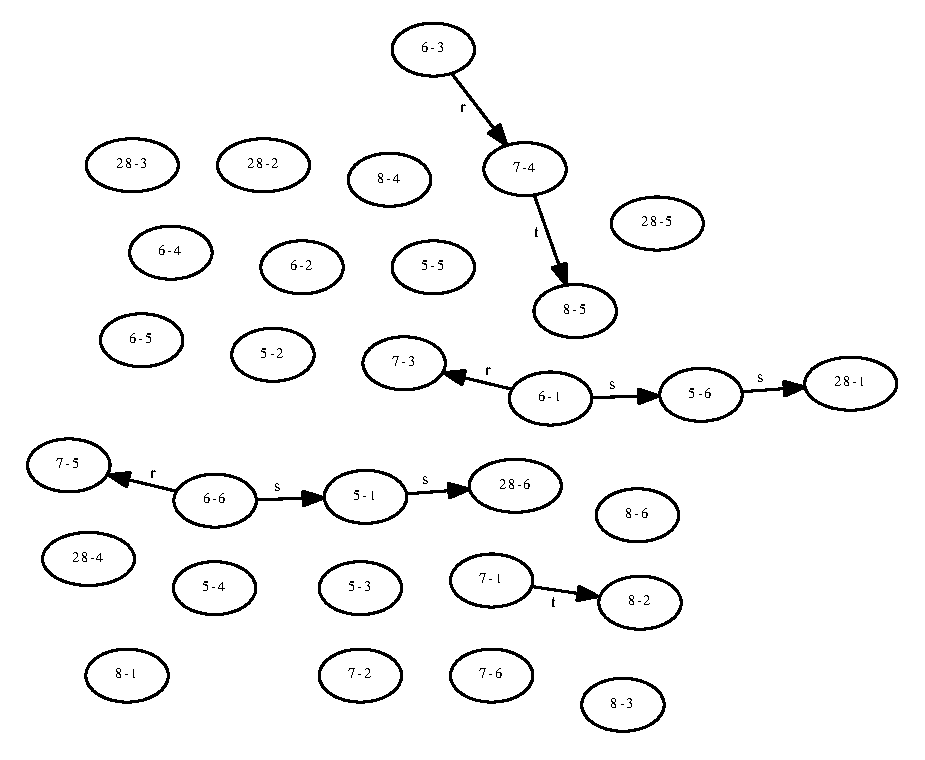
\includegraphics[scale=0.5, bb=0 0 400 410]{python/ex_K_i4-x-g.eps}
%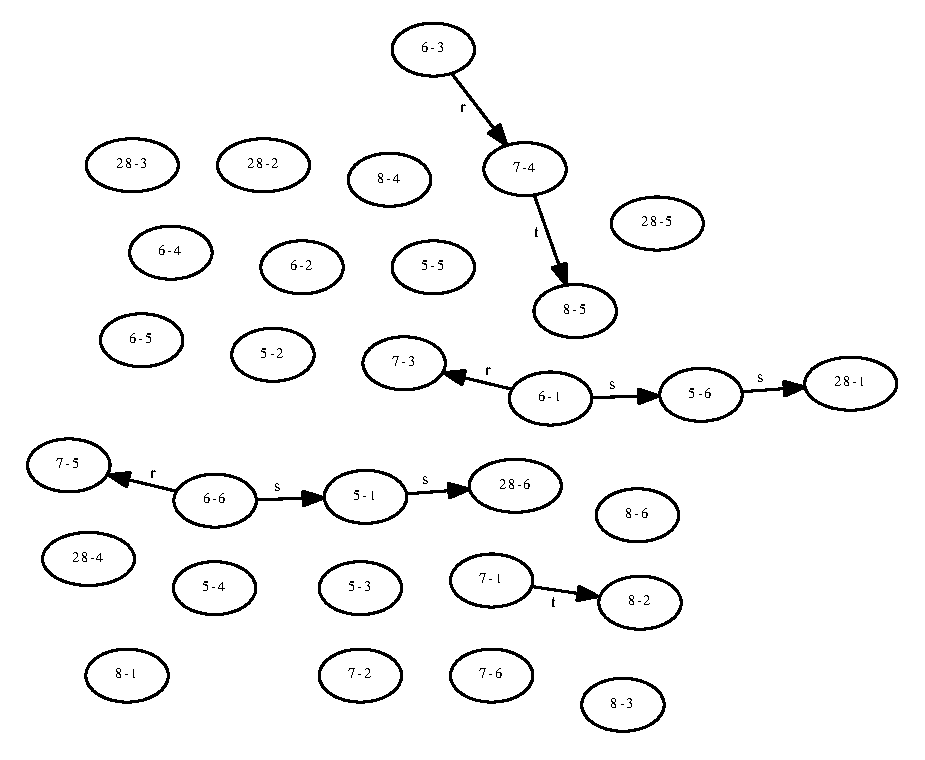
\includegraphics[scale=0.45]{python/ex_K_i4-x-g.eps}
\caption{$\cP_4^\prime=\Theta_4^\prime\times \G_{A_2}$}
\label{fig:K_i4-x-g}
\end{center}
\end{figure}

\begin{comment}
\begin{figure}
\begin{center}
\psfrag{a}{$x_1$}
\psfrag{b}{$x_2$}
\psfrag{c}{$x_3$}
\psfrag{r}{$y_1$}
\psfrag{s}{$y_2$}
\psfrag{t}{$y_3$}
\psfrag{x}{$z_1$}
\psfrag{y}{$z_2$}
\psfrag{z}{$z_3$}
\psfrag{u}{$y_4$}
\psfrag{1}{$1$}
%\begin{subfigure}[b]{.3\columnwidth}
%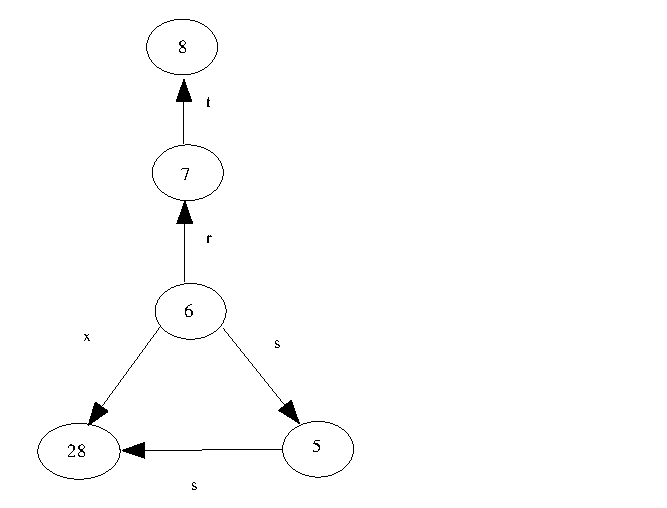
\includegraphics[scale=0.5, angle=90, bb=0 0  82 280]{python/ex_K_i4.eps}
%\caption{$\Theta_5^\prime$}
%\label{fig:KY15}
%\end{subfigure}
%\hspace*{2cm}
%\begin{subfigure}[b]{.3\columnwidth}
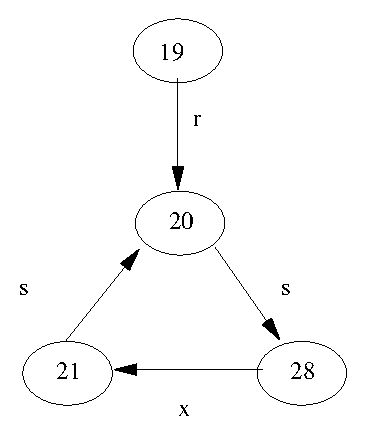
\includegraphics[scale=0.5, angle=90, bb=0 0 82 210]{python/ex_K_j4.eps}
\caption{$\Theta_5^{\prime\prime}$}
\label{fig:K_j4}
%\end{subfigure}
\end{center}
%\caption{Modified $X_2$ components}
%\label{fig:KY5}
\end{figure}
\end{comment}

\begin{figure}
\begin{center}
\psfrag{a}{\hspace{2pt}\small$x_1$}
\psfrag{a1}{\hspace*{-18pt}\small$x_1$}
\psfrag{a2}{\hspace*{-24pt}\raisebox{2pt}{\small$x_1$}}
\psfrag{a3}{\hspace*{2pt}\raisebox{-4pt}{\small$x_1$}}
\psfrag{a4}{\hspace*{10pt}\raisebox{0pt}{\small$x_1$}}
\psfrag{a5}{\hspace*{-4pt}\raisebox{-6pt}{\small$x_1$}}
\psfrag{a6}{\hspace*{-6pt}\raisebox{-10pt}{\small$x_1$}}
\psfrag{a7}{\hspace*{8pt}\raisebox{8pt}{\small$x_1$}}
\psfrag{a8}{\hspace*{-9pt}\raisebox{9pt}{\small$x_1$}}
\psfrag{a9}{\hspace*{-7pt}\raisebox{5pt}{\small$x_1$}}
\psfrag{a10}{\hspace*{0pt}\raisebox{-2pt}{\small$x_1$}}
\psfrag{a11}{\hspace*{-8pt}\raisebox{-8pt}{\small$x_1$}}
\psfrag{a12}{\hspace*{18pt}\raisebox{8pt}{\small$x_1$}}
\psfrag{b}{\hspace{2pt}\small$x_2$}
\psfrag{b1}{\hspace{2pt}\raisebox{-2pt}{\small$x_2$}}
\psfrag{b2}{\hspace{-12pt}\small$x_2$}
\psfrag{b3}{\hspace{-8pt}\raisebox{-8pt}{\small$x_2$}}
\psfrag{b4}{\hspace{-10pt}\raisebox{4pt}{\small$x_2$}}
\psfrag{b5}{\hspace{14pt}\raisebox{0pt}{\small$x_2$}}
\psfrag{b6}{\hspace{6pt}\raisebox{4pt}{\small$x_2$}}
\psfrag{b7}{\hspace{-12pt}\raisebox{-8pt}{\small$x_2$}}
\psfrag{b8}{\hspace{-2pt}\raisebox{8pt}{\small$x_2$}}
\psfrag{c}{\hspace{2pt}\small$x_3$}
\psfrag{c1}{\hspace{-14pt}\raisebox{-2pt}{\small$x_3$}}
\psfrag{c2}{\hspace{6pt}\raisebox{-6pt}{\small$x_3$}}
\psfrag{c3}{\hspace{2pt}\raisebox{-10pt}{\small$x_3$}}
\psfrag{c4}{\hspace{-8pt}\raisebox{0pt}{\small$x_3$}}
\psfrag{c5}{\hspace{-2pt}\raisebox{-4pt}{\small$x_3$}}
\psfrag{r}{\hspace{2pt}\small$y_1$}
\psfrag{r1}{\hspace{8pt}\small$y_1$}
\psfrag{s}{\hspace{2pt}\small$y_2$}
\psfrag{s1}{\hspace{-10pt}\raisebox{2pt}{\small$y_2$}}
\psfrag{t}{\hspace{2pt}\small$y_3$}
\psfrag{t1}{\hspace{8pt}\small$y_3$}
\psfrag{x}{\hspace{2pt}\small$z_1$}
\psfrag{x1}{\hspace{-15pt}\small$z_1$}
\psfrag{x2}{\hspace{-20pt}\raisebox{0pt}{\small$z_1$}}
\psfrag{x3}{\hspace{2pt}\raisebox{6pt}{\small$z_1$}}
\psfrag{x4}{\hspace{8pt}\raisebox{0pt}{\small$z_1$}}
\psfrag{x5}{\hspace{-8pt}\raisebox{8pt}{\small$z_1$}}
\psfrag{x6}{\hspace*{-7pt}\raisebox{0pt}{\small$z_1$}}
\psfrag{x7}{\hspace*{2pt}\raisebox{0pt}{\small$z_1$}}
\psfrag{x8}{\hspace*{4pt}\raisebox{-8pt}{\small$z_1$}}
\psfrag{x9}{\hspace*{-12pt}\raisebox{6pt}{\small$z_1$}}
\psfrag{x10}{\hspace*{-8pt}\raisebox{4pt}{\small$z_1$}}
\psfrag{y}{\hspace{2pt}\small$z_2$}
\psfrag{y1}{\hspace{-18pt}\small$z_2$}
\psfrag{y2}{\hspace{2pt}\raisebox{6pt}{\small$z_2$}}
\psfrag{y3}{\hspace{8pt}\raisebox{0pt}{\small$z_2$}}
\psfrag{y4}{\hspace{2pt}\raisebox{-10pt}{\small$z_2$}}
\psfrag{y5}{\hspace{-10pt}\raisebox{0pt}{\small$z_2$}}
\psfrag{y6}{\hspace{-6pt}\raisebox{0pt}{\small$z_2$}}
\psfrag{y7}{\hspace{-4pt}\raisebox{6pt}{\small$z_2$}}
\psfrag{y8}{\hspace{-18pt}\raisebox{8pt}{\small$z_2$}}
\psfrag{z}{\hspace{2pt}\small$z_3$}
\psfrag{z1}{\hspace{-16pt}\small$z_3$}
\psfrag{z2}{\hspace{-8pt}\raisebox{-6pt}{\small$z_3$}}
\psfrag{z3}{\hspace{-30pt}\small$z_3$}
\psfrag{z4}{\hspace{8pt}\small$z_3$}
\psfrag{z5}{\hspace{-8pt}\raisebox{3pt}{\small$z_3$}}
\psfrag{z6}{\hspace{6pt}\raisebox{-9pt}{\small$z_3$}}
\psfrag{u}{\hspace{2pt}\small $y_4$}
\psfrag{u1}{\hspace{-6pt}\raisebox{4pt}{\small $y_4$}}
\psfrag{u2}{\hspace{2pt}\raisebox{-10pt}{\small $y_4$}}
\psfrag{1}{\hspace{-1pt}\raisebox{-2pt}{\scriptsize $1$}}
\psfrag{2}{\hspace{-1pt}\raisebox{-2pt}{\scriptsize $2$}}
\psfrag{3}{\hspace{-1pt}\raisebox{-2pt}{\scriptsize $3$}}
\psfrag{4}{\hspace{-1pt}\raisebox{-2pt}{\scriptsize $4$}}
\psfrag{5}{\hspace{-1pt}\raisebox{-2pt}{\scriptsize $5$}}
\psfrag{6}{\hspace{-1pt}\raisebox{-2pt}{\scriptsize $6$}}
\psfrag{7}{\hspace{-1pt}\raisebox{-2pt}{\scriptsize $7$}}
\psfrag{8}{\hspace{-1pt}\raisebox{-2pt}{\scriptsize $8$}}
\psfrag{9}{\hspace{-1pt}\raisebox{-2pt}{\scriptsize $9$}}
\psfrag{10}{\hspace{-2pt}\raisebox{-2pt}{\scriptsize $10$}}
\psfrag{11}{\hspace{-2pt}\raisebox{-2pt}{\scriptsize $11$}}
\psfrag{12}{\hspace{-2pt}\raisebox{-2pt}{\scriptsize $12$}}
\psfrag{13}{\hspace{-2pt}\raisebox{-2pt}{\scriptsize $13$}}
\psfrag{14}{\hspace{-2pt}\raisebox{-2pt}{\scriptsize $14$}}
\psfrag{15}{\hspace{-2pt}\raisebox{-2pt}{\scriptsize $15$}}
\psfrag{16}{\hspace{-2pt}\raisebox{-2pt}{\scriptsize $16$}}
\psfrag{17}{\hspace{-2pt}\raisebox{-2pt}{\scriptsize $17$}}
\psfrag{18}{\hspace{-2pt}\raisebox{-2pt}{\scriptsize $18$}}
\psfrag{19}{\hspace{-2pt}\raisebox{-2pt}{\scriptsize $19$}}
\psfrag{20}{\hspace{-2pt}\raisebox{-2pt}{\scriptsize $20$}}
\psfrag{21}{\hspace{-2pt}\raisebox{-2pt}{\scriptsize $21$}}
\psfrag{22}{\hspace{-2pt}\raisebox{-2pt}{\scriptsize $22$}}
\psfrag{23}{\hspace{-2pt}\raisebox{-2pt}{\scriptsize $23$}}
\psfrag{24}{\hspace{-2pt}\raisebox{-2pt}{\scriptsize $24$}}
\psfrag{25}{\hspace{-2pt}\raisebox{-2pt}{\scriptsize $25$}}
\psfrag{26}{\hspace{-2pt}\raisebox{-2pt}{\scriptsize $26$}}
\psfrag{27}{\hspace{-2pt}\raisebox{-2pt}{\scriptsize $27$}}
\psfrag{28}{\hspace{-2pt}\raisebox{-2pt}{\scriptsize $28$}}
\psfrag{29}{\hspace{-2pt}\raisebox{-2pt}{\scriptsize $29$}}
\psfrag{30}{\hspace{-2pt}\raisebox{-2pt}{\scriptsize $30$}}
\psfrag{31}{\hspace{-2pt}\raisebox{-2pt}{\scriptsize $31$}}
\psfrag{32}{\hspace{-2pt}\raisebox{-2pt}{\scriptsize $32$}}
\psfrag{33}{\hspace{-2pt}\raisebox{-2pt}{\scriptsize $33$}}
\psfrag{34}{\hspace{-2pt}\raisebox{-2pt}{\scriptsize $34$}}
\psfrag{35}{\hspace{-2pt}\raisebox{-2pt}{\scriptsize $35$}}
\psfrag{36}{\hspace{-2pt}\raisebox{-2pt}{\scriptsize $36$}}
\psfrag{37}{\hspace{-2pt}\raisebox{-2pt}{\scriptsize $37$}}
\psfrag{38}{\hspace{-2pt}\raisebox{-2pt}{\scriptsize $38$}}
\psfrag{39}{\hspace{-2pt}\raisebox{-2pt}{\scriptsize $39$}}
\psfrag{40}{\hspace{-2pt}\raisebox{-2pt}{\scriptsize $40$}}
\psfrag{41}{\hspace{-2pt}\raisebox{-2pt}{\scriptsize $41$}}
\psfrag{42}{\hspace{-2pt}\raisebox{-2pt}{\scriptsize $42$}}
\psfrag{43}{\hspace{-2pt}\raisebox{-2pt}{\scriptsize $43$}}
\psfrag{44}{\hspace{-2pt}\raisebox{-2pt}{\scriptsize $44$}}
\psfrag{45}{\hspace{-2pt}\raisebox{-2pt}{\scriptsize $45$}}
\psfrag{46}{\hspace{-2pt}\raisebox{-2pt}{\scriptsize $46$}}
\psfrag{47}{\hspace{-2pt}\raisebox{-2pt}{\scriptsize $47$}}
\psfrag{48}{\hspace{-2pt}\raisebox{-2pt}{\scriptsize $48$}}
\psfrag{49}{\hspace{-2pt}\raisebox{-2pt}{\scriptsize $49$}}
\psfrag{50}{\hspace{-2pt}\raisebox{-2pt}{\scriptsize $50$}}
\psfrag{51}{\hspace{-2pt}\raisebox{-2pt}{\scriptsize $51$}}
\psfrag{52}{\hspace{-2pt}\raisebox{-2pt}{\scriptsize $52$}}
\psfrag{53}{\hspace{-2pt}\raisebox{-2pt}{\scriptsize $53$}}
\psfrag{54}{\hspace{-2pt}\raisebox{-2pt}{\scriptsize $54$}}
\psfrag{55}{\hspace{-2pt}\raisebox{-2pt}{\scriptsize $55$}}
\psfrag{56}{\hspace{-2pt}\raisebox{-2pt}{\scriptsize $56$}}
\psfrag{57}{\hspace{-2pt}\raisebox{-2pt}{\scriptsize $57$}}
\psfrag{58}{\hspace{-2pt}\raisebox{-2pt}{\scriptsize $58$}}
\psfrag{59}{\hspace{-2pt}\raisebox{-2pt}{\scriptsize $59$}}
%\hspace*{-3em}
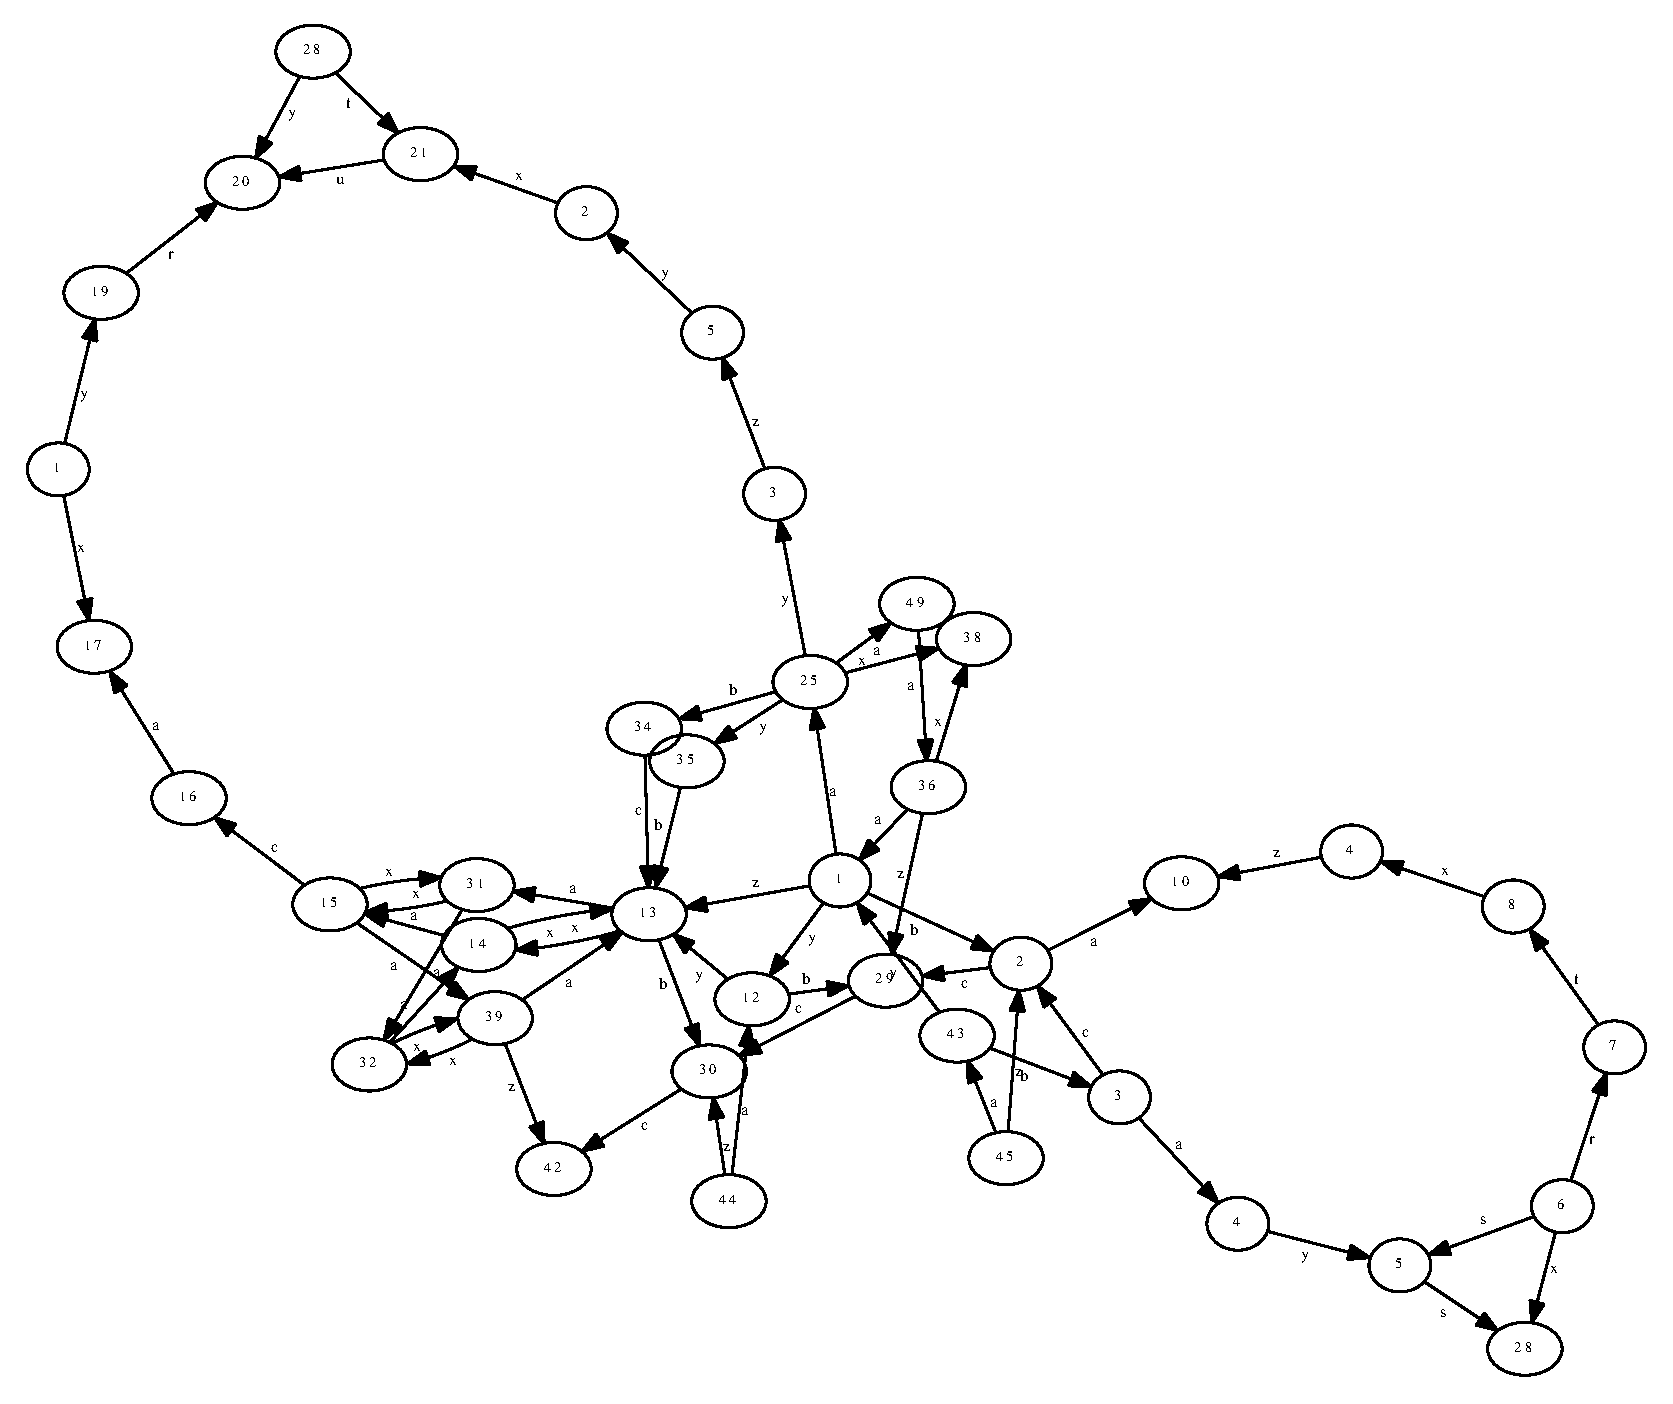
\includegraphics[width=\textwidth, height=.9\textheight, keepaspectratio=false]{python/ex_K_reassembly.eps}
%\hspace*{-3em}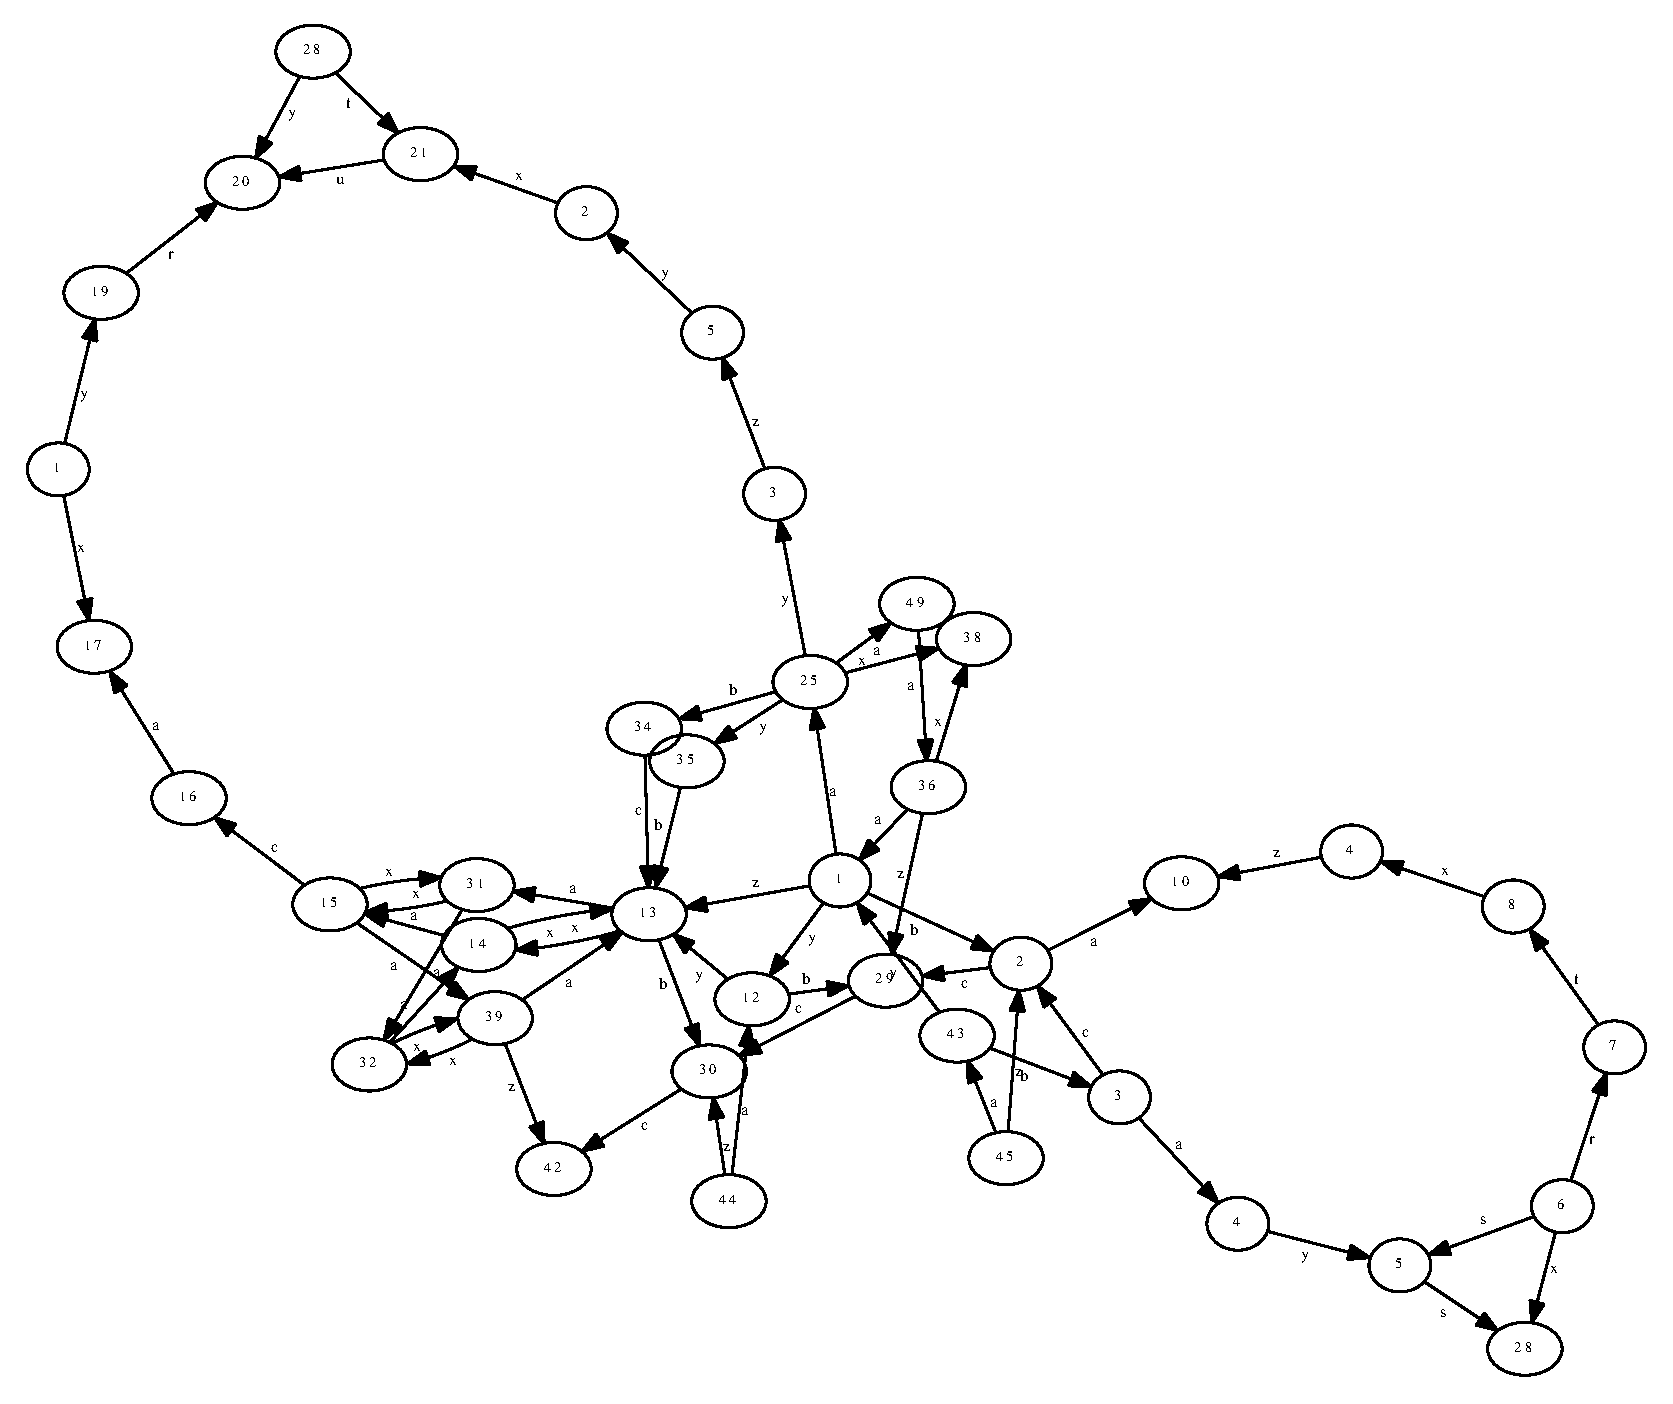
\includegraphics[scale=.5]{python/ex_K_reassembly.eps}
%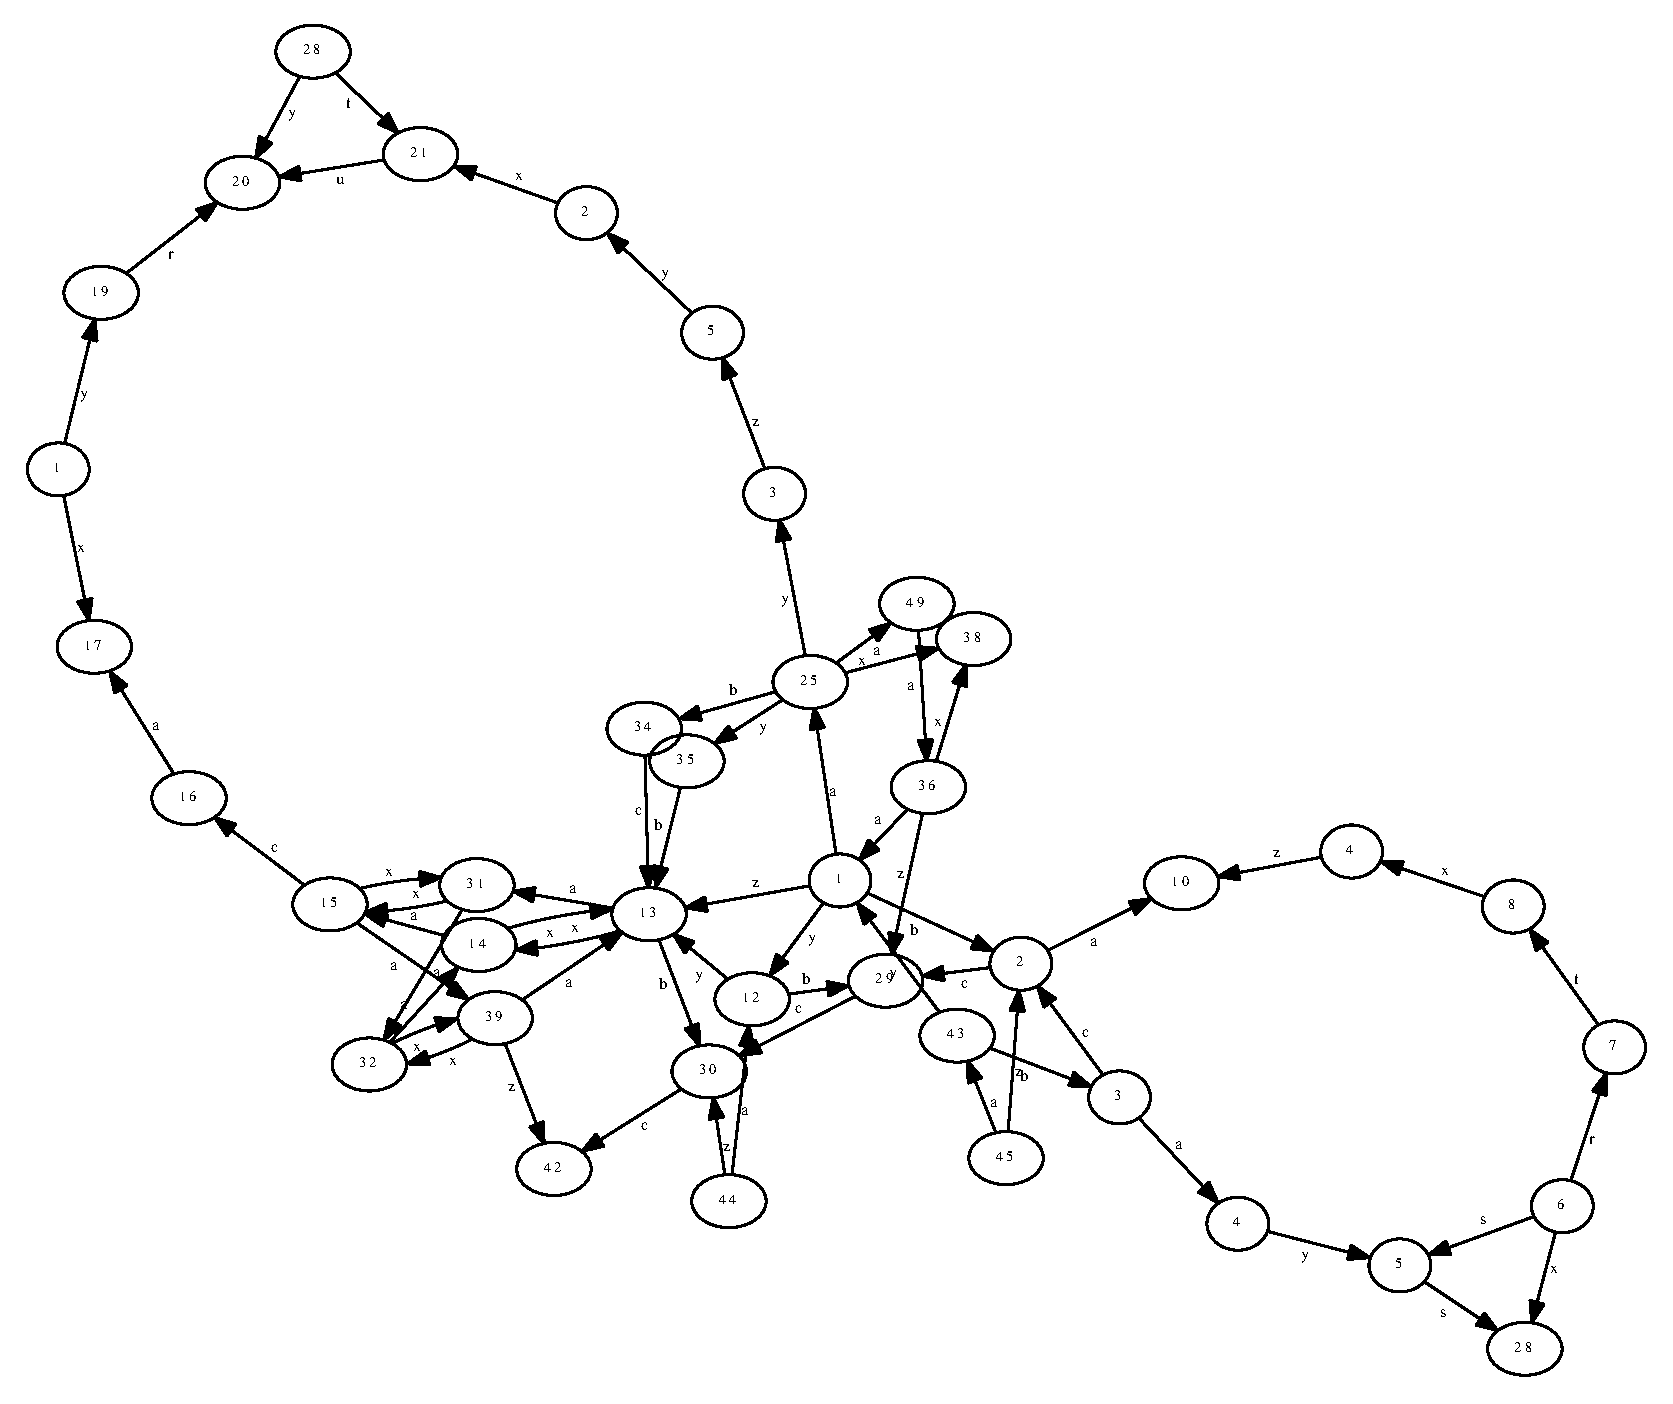
\includegraphics[scale=1.2,bb=36 36 432 370]{python/ex_K_reassembly.eps}
\caption{$\Psi$}
\label{fig:out}
\end{center}
\end{figure}
\section{Proofs of main results}
\begin{lemma}\label{lem:nfcomp}
Let $\a$ and $\b$ be boundary vertices of  an $X_k$ component $\T$ of
an inverse automaton $\D$, with alphabet $\S$. Then   the following hold.
\be
\item\label{it:nfcomp1}
  $\pi(L(\T,\a,\b))=\pi(L(\T_5,\theta(\a),\theta(\b)))$.
\item\label{it:nfcomp2} Let $w$ be a word
 which is accepted by the automaton $(\T, \a, \b)$. Then the
normal form of $w$ is accepted by $(\T_5, \theta(\a), \theta(\b))$.
\ee
\end{lemma}
\begin{proof} ~
\ref{it:nfcomp1}.
At each stage of the modification process of Algorithm
II the image under $\pi$ of the language accepted by $(\T_i,\a,\b)$  was
preserved.

\ref{it:nfcomp2}.
We may assume that $w\in \FF(X_k)$ (given the construction of $\T_1$).
Let $w$ have normal form $h_1s h_2^{-1}$, where $s\in S_k$ and $h_i\in \FF(Z)$.
There are two cases to consider, depending on whether $s$ is a
representative of type $1$ or type $2$.
 First consider the case where $s$ is of type $1$, say
 $s= a_1 e a_2^{-1}$, where
$a_1$ is a maximal $L_{Q_k}$-prefix and an $L_{T_k}$-prefix of $s$ and
 $a_2$  is a maximal $L_{Q_k}$-prefix and an $L_{T_k}$-prefix of $a_2\circ e^{-1}$.
 Then, as the normal form is the result of applying $\phi_k$ to the
output of Algorithm I,
 there are words
$g_1, g_2, b_1$ and $b_2\in \FF(X_k)$ such that
$w=g_1\circ b_1\circ e \circ b_2^{-1}\circ g_2^{-1}$,
$g_i\in H_k$, $b_1$ is a maximal $L_Q$-prefix of
$b_1\circ e \circ b_2^{-1}\circ g_2^{-1}$,
$b_2$ is a maximal $L_Q$-prefix of $b_2\circ e^{-1}$, $e\neq 1$,
$a_i=w(\t(b_i))$ and $\phi_k(h_i)=g_ib_ia_i^{-1}$, $i=1,2$.

Recall that we refer to the images of vertices of $\T$ in $\T_i$ as
 ``vertices of $\T$'', for $i=1,\ldots ,5$.
Since $g_i\in H_k$ and $w$ is accepted by $\T_1$ there is a path
labelled $g_1$ from $\a$ to a vertex $\a_1$ of $\T$ and a path
labelled $g_2$ from $\b$ to a vertex $\b_1$ of $\T$. Therefore, in $\cP$,
there are paths $p_1$ from $(\a,1)$ to $(\a_1,1)$ labelled $g_1$, and
$p_2$
from $(\b,1)$ to $(\b_1,1)$ labelled $g_2$.
(See Figure \ref{fig:nf-1}.)
\begin{figure}
\begin{center}
\psfrag{a}{$\a$}
\psfrag{b}{$\b$}
\psfrag{a1}{$\a_1$}
\psfrag{a2}{$\a_2$}
\psfrag{b1}{$\b_1$}
\psfrag{b2}{$\b_2$}
\psfrag{b_1}{$b_1$}
\psfrag{b_2}{$b_2$}
\psfrag{h1}{$h_1$}
\psfrag{c}{$e$}
\psfrag{w'1}{$w_1^\prime$}
\psfrag{w'2}{$w_2^\prime$}
\psfrag{s}{$s$}
\psfrag{h2}{$h_2$}
\psfrag{g1}{$\phi_k^{-1}(g_1)$}
\psfrag{g2}{$\phi_k^{-1}(g_2)$}
\psfrag{h'2a2}{$h_2^\prime a_2$}
\psfrag{h'1a1}{$h_1^\prime a_1$}
\psfrag{Th5}{$\T_4$}
\psfrag{cP}{$\cP_3$}
\psfrag{G_A}{$\G_{A_k}$}
\psfrag{(a,1)}{$(\a,1)$}
\psfrag{(a1,1)}{$(\a_1,1)$}
\psfrag{(a2,e1)}{$(\a_2,\e_1)$}
\psfrag{(b,1)}{$(\b,1)$}
\psfrag{(b1,1)}{$(\b_1,1)$}
\psfrag{(b2,e2)}{$(\b_2,\e_2)$}
\psfrag{g-1}{$g_1$}
\psfrag{g-2}{$g_2$}
\psfrag{b'_1}{$b_1^\prime$}
\psfrag{b'_2}{$b_2^\prime$}
\psfrag{a_1}{$a_1$}
\psfrag{a_2}{$a_2$}
\psfrag{e1}{$\e_1$}
\psfrag{e2}{$\e_2$}
\psfrag{r1}{$g_1$}
\psfrag{r2}{$g_2$}
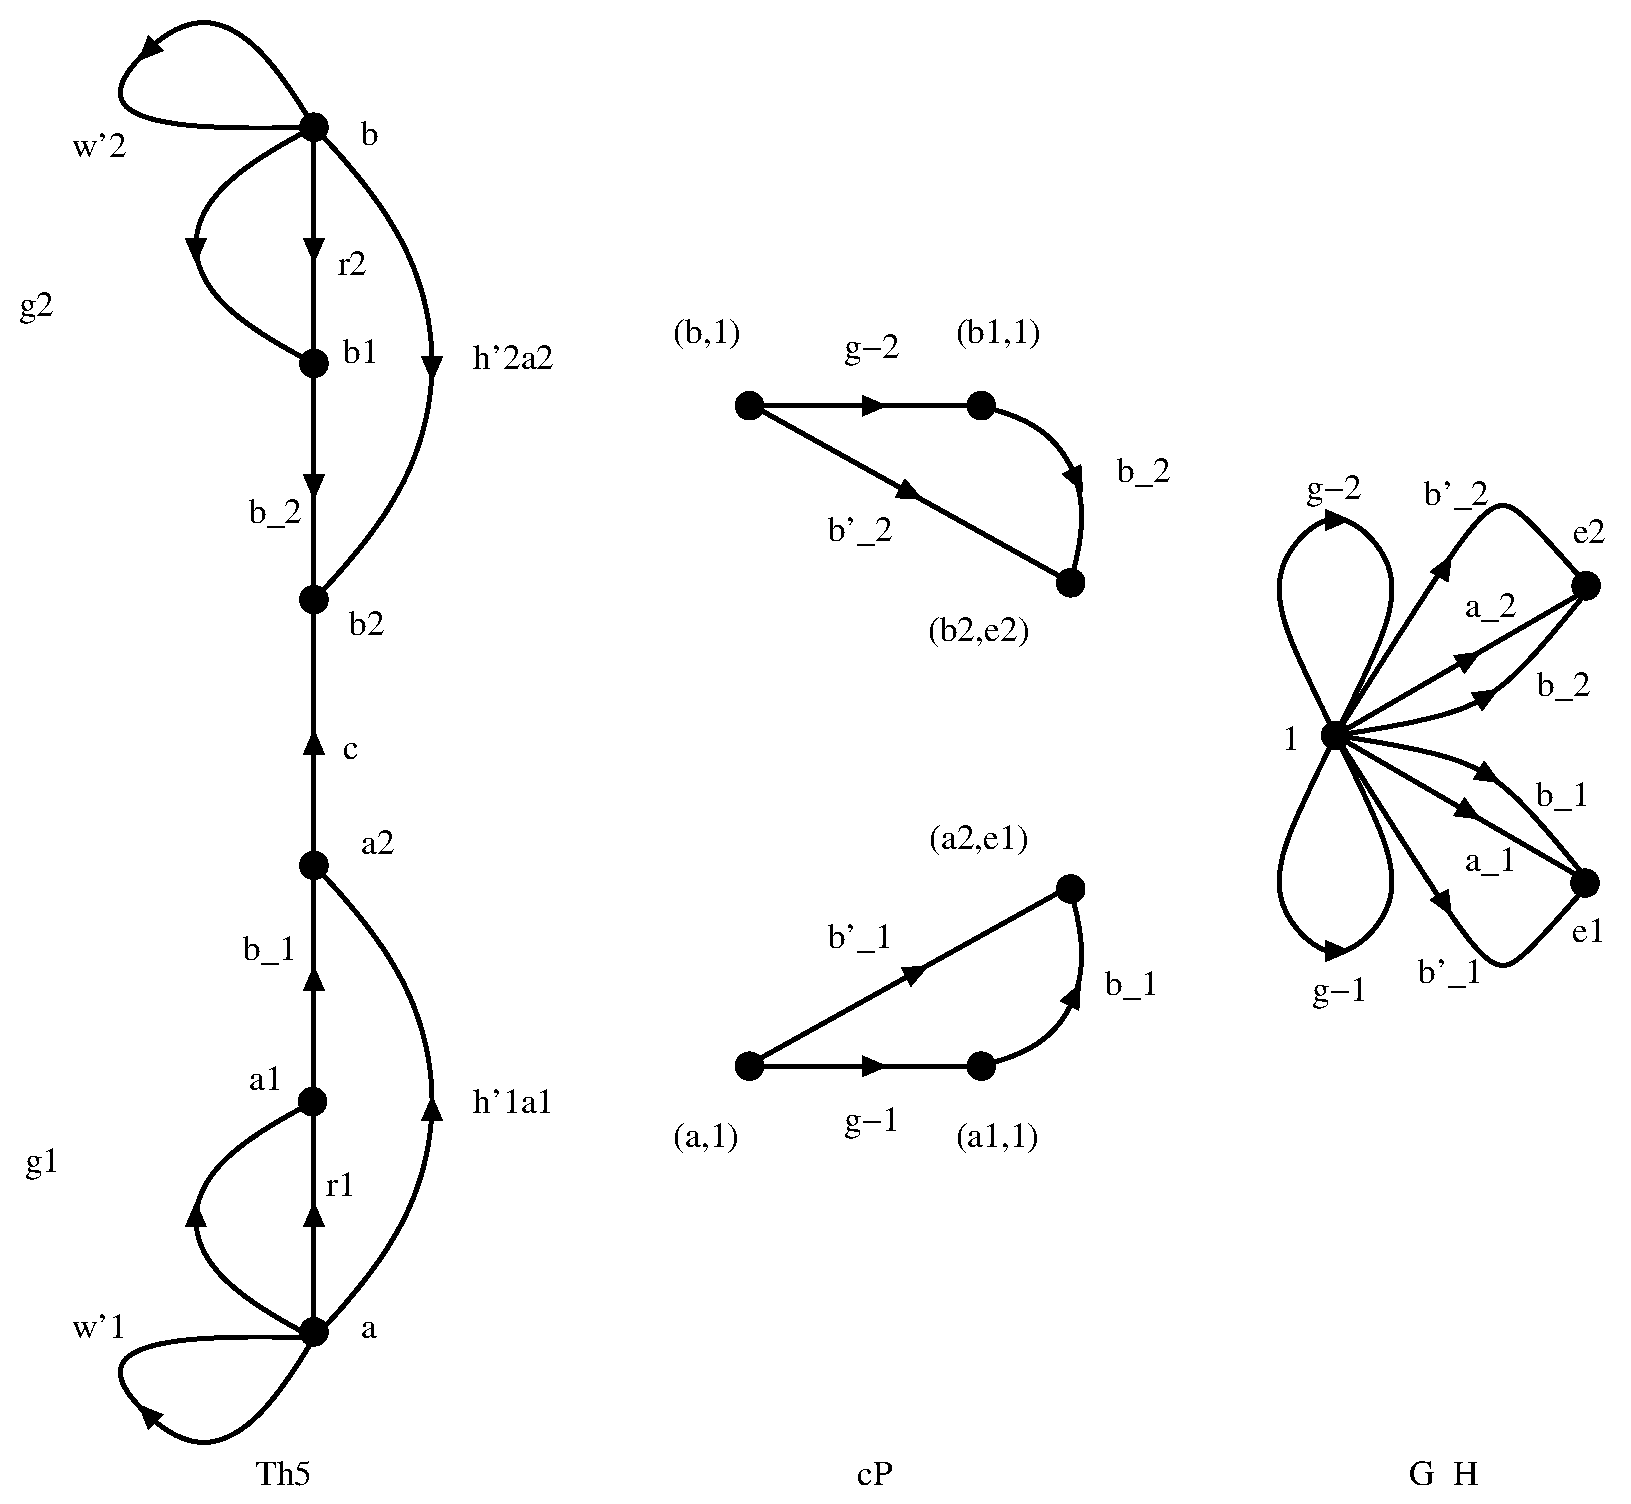
\includegraphics[scale=.5]{nf-1.eps}
\end{center}
\caption{Normal form: type 1.}
\label{fig:nf-1}
\end{figure}
Now $p_1$ may
be written as a concatenation of paths $p_1=o_0e_1\cdots e_l o_{l}$,
where $o_i$ is a simple path in $\U$ and $e_i$ is an edge of $\cP$ which does
not belong to $\U$.  Let $e_i$ have initial and terminal vertices
$\g_i$ and $\d_i$, and let $L_i$ and $R_i$ be the simple paths in $\U$ from
$(\a,1)$ to $\g_i$ and from $\d_i$ to $(\a,1)$, respectively.
In addition let $L_{l+1}$ be the path in $\U$ from $(\a,1)$ to
$(\a_1,1)$.
Then $L_1=o_0$ and, for $i=1,\ldots ,l$, $L_{i+1}=R_i^{-1}o_{i}$.
(See Figure \ref{fig:LeR}.)
\begin{figure}
\begin{center}
\psfrag{R1}{$R_1$}
\psfrag{L1}{$L_1$}
\psfrag{e1}{$e_1$}
\psfrag{o1}{$o_1$}
\psfrag{R2}{$R_2$}
\psfrag{L2}{$L_2$}
\psfrag{e2}{$e_2$}
\psfrag{o2}{$o_2$}
\psfrag{Rl}{$R_l$}
\psfrag{Ll}{$L_l$}
\psfrag{el}{$e_l$}
\psfrag{ol}{$o_l$}
\psfrag{o0}{$o_0$}
\psfrag{ol-}{$o_{l-1}$}
\psfrag{(a,1)}{$(\a,1)$}
\psfrag{(a1,1)}{$(\a_1,1)$}
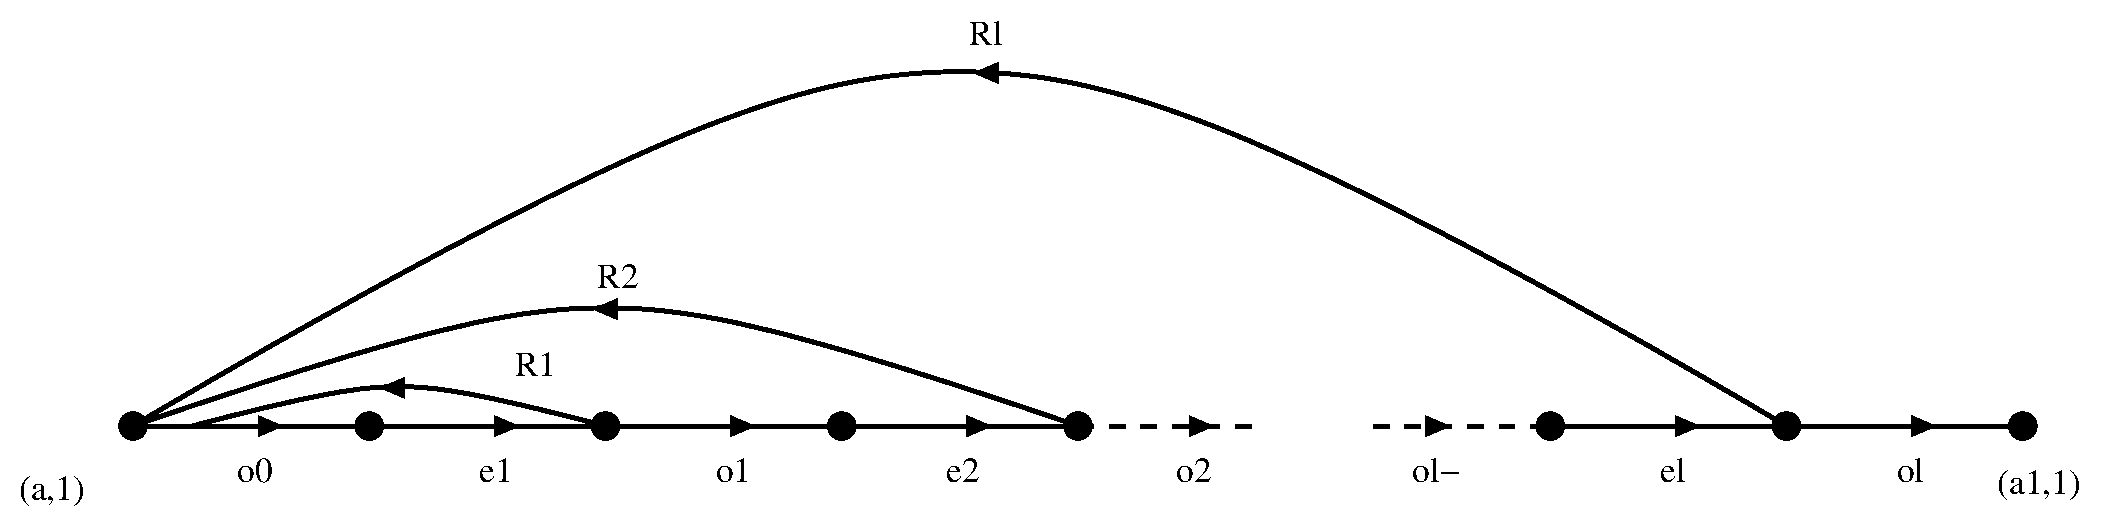
\includegraphics[scale=.4]{LeR.eps}
\end{center}
\caption{The path $p_1$.}
\label{fig:LeR}
\end{figure}
Moreover, for $i=1,\ldots ,l$,
the path $L_i e_i R_i$ is a closed path in $\cP$, based
at $(\a,1)$, containing exactly one edge, $e_i$, which is not in $\U$.
Thus the label of  $L_i e_i R_i$ is $v_i\in H_k$ and $\phi_k^{-1}(v_i)$ is the
label of a closed path in $\T_3$, based at  $\a$. (All such paths
were added in the construction of $\T_3$ from $\T_2$.)
Also, the path $L_{l+1}$, from $(\a,1)$ to $(\a_1,1)$, has
label $v_{l+1}\in H$,
and by construction of $\T_2$ there is a path from $\a$ to
$\a_1$ in $\T_2$ with label $\phi_k^{-1}(v_{l+1})$.
The path
$p_1$ is the result of reducing (deleting adjacent edges $e,e^{-1}$) the path
$o_0 e_1 (R_1 R_1^{-1}) o_1 \cdots e_{l}(R_l R_l^{-1}) o_{l}$, which
is equal to the path $L_1 e_1 R_1 \cdots L_l e_l R_l L_{l+1}$. Hence the label $g_1$
of $p_1$ is the result of
reducing the word $v_1\cdots v_l v_{l+1}$
 and $\phi_k^{-1}(g_1)$ is the result of
reducing $\phi_k^{-1}(v_1) \cdots \phi_k^{-1}(v_{l+1})$. As each $\phi_k^{-1}(v_i)$ is readable
in $\T_3$ and $\T_3$ is folded this means  that $\phi_k^{-1}(g_1)$ is the
label of a path, from $\a$ to   $\a_1$, in $\T_3$. Similarly,
$\phi_k^{-1}(g_2)$
is the label of a path from $\b$ to $\b_1$ in $\T_3$.

The word $b_1$ is readable by $\G_{A_k}$ and there
is a path with label $b_1$ in $\T_1$ from $\a_1$ to some vertex $\a_2$
of $\T$.
Hence $b_1$ is the label of a path in $\cP$ from $(\a_1,1)$ to
$(\a_2,\e_1)$, for some vertex $\e_1$ of $\G_{A_k}$.
By definition $a_1=w(\t(b_1))$ is the label of a path in $T_k$ from $1$ to $\e_1$.
Let $b_1^\prime$
 be the label of the simple path $p_1^\prime$ in $\U$ from
$(\a_1,1)$ to $(\a_2,\e_1)$ (see Figure \ref{fig:nf-1}). By construction $\T_4$ contains a path
from $\a_1$ to $\a_2$ with label $h_1^\prime a_1$, where
$h_1^\prime =\phi_k^{-1}(b_1^\prime a_1^{-1})\in \FF(Z)$.
(If $\cP$ covers the pair $(\a_1,1)$, $(\a_2,\e_1)$ then
$b_1^\prime=a_1$ and $h_1^\prime$ is the empty word, while there
exists a path with label $a_1$ from $\a_1$ to $\a_2$ in $\T_3$.)
%Furthermore we have
%$\pi(\phi_k(h_1^\prime)b_1^{\prime\prime})=\pi(b_1^\prime)$.
Now $b_1(b_1^\prime)^{-1}\in H_k$ and is the label of a closed
path  in $\cP$ based at $(\a_1,1)$; so by the
previous part of proof, $\T_3$ contains a closed path, based at $\a_1$,
 with label
$w_1^\prime=\phi_k^{-1}(b_1(b_1^\prime)^{-1})$. Hence, as it is folded,
$\T_4$ contains a path, from $\a$ to $\a_2$,
with label the reduced word obtained from the product
$\phi_k^{-1}(g_1)w_1^{\prime} h_1^\prime a_1$, that is
 $\phi_k^{-1}(g_1b_1a_1^{-1}) a_1=h_1a_1$.
 Similarly, $\T_1$ contains a path labelled $b_2$ from $\b_1$ to
some vertex $\b_2$ of $\T$, and $\T_4$ contains a path from
$\b$ to $\b_2$ with label $h_2a_2$.

As $w$ is the label of a path in $\T_1$ there is a path from $\a_2$ to
$\b_2$ in $\T_4$ with label $e$. Therefore, in this case, $\T_4$ contains
a path from $\a$ to $\b$ which has label the normal form of $w$.



In the second case,
let $w$ have normal form $h_1 a_1 a_2^{-1} h_2^{-1} $, where
$h_1$ and $h_2$ are in $\FF(Z)$,  $a_1$ and $a_2$ are labels
of simple paths in the subtree $T_k$ and $s=a_1a_2^{-1}$ is a double coset
representative of type $2$. Then there are words
$g_1, g_2, b_1, b_2, c$  in $\FF(X_k)$,  such that
$w=g_1\circ b_1 \circ b_2^{-1}\circ g_2^{-1}$,
$g_i\in H_k$, $b_1$ is a maximal $L_Q$-prefix of
$b_1 \circ b_2^{-1}\circ g_2^{-1}$, $b_2$ in
$L_Q$, $c=c(\t(b_1),\t(b_2))$, $a_i=w(v_i)$, where
$(v_1,v_2)$ is the $\sim$ representative of $(\t(b_1),\t(b_2))$, 
and $h_i=\phi_k^{-1}(g_ib_ica_i^{-1})$.

Then $\T$ contains vertices $\g_1=\a,\g_2=\b, \a_1, \a_2$ and $\g$ and there are paths
in $\T_1$ 
labelled $g_i$, from $\g_i$ to $\a_i$, and labelled $b_i$ from $\a_i$ to $\g$,
$i=1,2$. Moreover, as in the first case there are paths in $\T_3$ labelled
$\phi_k^{-1}(g_i)$
from $\g_i$ to $\a_i$, $i=1,2$.
(See Figure \ref{fig:nf-2}.)
\begin{figure}
\begin{center}
\psfrag{a}{$\a=\g_1$}
\psfrag{b}{$\b=\g_2$}
\psfrag{a1}{$\a_1$}
\psfrag{a2}{$\a_2$}
\psfrag{b1}{$\a_2$}
\psfrag{b2}{$\b_2$}
\psfrag{g1}{$\phi_k^{-1}(g_1)$}
\psfrag{g2}{$\phi_k^{-1}(g_2)$}
\psfrag{Th5}{$\T_5$}
\psfrag{b_1}{$b_1$}
\psfrag{b_2}{$b_2$}
\psfrag{w}{$r$}
\psfrag{r1}{$g_1$}
\psfrag{r2}{$g_2$}
\psfrag{m}{$\g$}
\psfrag{bt1}{$\phi_k^{-1}(b_1 t_1^{-1})$}
\psfrag{bt2}{$\phi_k^{-1}(b_2 t_2^{-1})$}
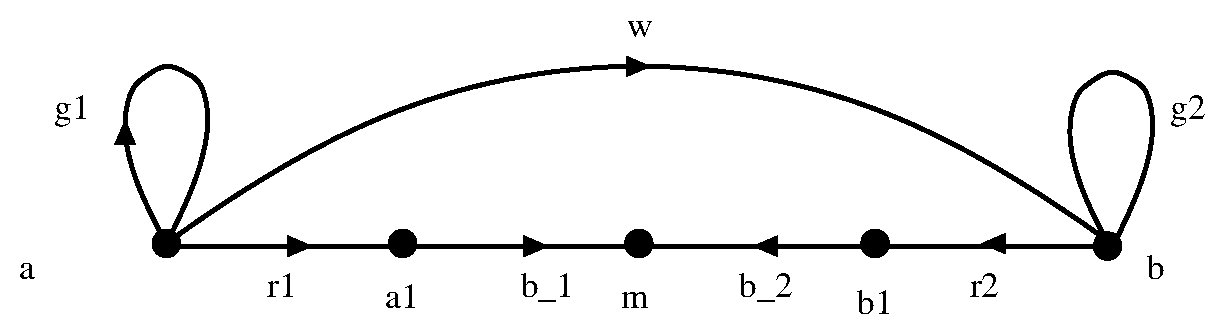
\includegraphics[scale=.5]{nf-2.eps}
\end{center}
\caption{Normal form: type 2, $r=\phi_k^{-1}(t_1ca_1^{-1})a_1a_2^{-1}\phi_k^{-1}(a_2c^{-1}t_2^{-1})$.}
\label{fig:nf-2}
\end{figure}
Let $\e_i=\t(b_i)$, $i=1,2$; so $(\e_1,\e_2)\in P$. 
As $w$ is readable in $\T_1$ there is a path labelled 
$b_i$ from $(\a_i,1)$ to $(\g,\e_i)$ in $\cP_{k,4}$, so there
exists a simple path, labelled $t_i$, from $(\a_i,1)$ to $(\g,\e_i)$ in 
$\U_{k,4}$. Then $\T_3$ contains a path from $\a_i$ to $\a_i$ with 
label $\phi_k^{-1}(b_it_i^{-1})$. 
By construction of $\T_5$ there is also a path labelled
$r=\phi_k^{-1}(t_1ca_1^{-1})a_1a_2^{-1}\phi_k^{-1}(a_2c^{-1}t_2^{-1})$
from $\a_1$ to $\a_2$.
 As $\T_5$ is folded
$
\phi_k^{-1}(g_1 b_1ca_1^{-1})a_1a_2^{-1}\phi_k^{-1}(a_2c^{-1}b_2^{-1}g_2)$
 is readable in
$\T_5$, as required.

\end{proof}

\begin{lemma}\label{lem:idverts}
Let $\theta$ be the map from $\D'$ to $\D'_5$ defined in the reassembly
phase of Algorithm II, in Section \ref{sec:dca}, and 
let $\approx$ be the equivalence relation on $V(\D^\prime_5)$, defined 
in \ref{it:R1}, above. For $v\in V(\D^\prime_5)$, 
let $[v]$ denote the equivalence class of $v$ under $\approx$. 
\be
\item
The graph $\D''$ defined in Section \ref{sec:dca} is isomorphic
to the graph output by  Step \ref{it:C19} of Algorithm II as described in
Section \ref{sub:summaryII}. 
\item
If $x$ and $y$ are vertices of $\D^\prime$, such that
$[\theta(x)]= [\theta(y)]$ in $\D^{\prime\prime}$, then
there exists a path in $\D$, from $\nu(x)$ to $\nu(y)$, with label $w$,
such that $\pi(w)=1$.
\ee
\end{lemma}
\begin{proof}
\be
\item
The Steps of Algorithm II in Section \ref{sub:summaryII}, as far as 
Step \ref{it:C16.5} carry out Modifications 1 to 5, as described in
Section \ref{sec:dca}. Thus the 
two versions of the graph $\D'$,
the first defined in Section \ref{sec:dca} and the second in
Section \ref{sub:summaryII}, are the same. 
We need then to  show that the quotient $\D''$ of 
 $\D'$ constructed in Section \ref{sec:dca} is isomorphic to
the graph output by Step \ref{it:C19} of the algorithm in 
Section \ref{sub:summaryII}. 
To avoid ambiguity the graph output by Step \ref{it:C19} will be
called $\hat\D''$ here. In the process of constructing $\hat\D''$
from $\D'$, two vertices $u$ and $v$ of $\D'$ are identified
if and only if there is a sequence $u=u_0,\ldots ,u_n=v$, such 
that $\vim(u_{i-1})\cap \vim(u_ i)\neq \emptyset$,  $i=1,\ldots , n$. 
Moreover, if the vertex $w$ of $\hat\D''$ is the result of identifying 
exactly $n$ vertices $v_1,\ldots ,v_n$ of $\D'$, then 
$\vim(w)=\cup_{i=1}^n\vim(v_i)$ and also, if $w$ and $w'$ are distinct
vertices of $\hat \D''$ then $\vim(w)\cap \vim(w')=\emptyset$. 
This being the case we  
 let  $\bowtie$ denote the equivalence relation on vertices of $\D'$ 
generated  by setting $\a\bowtie \b$ if and only if  $\vim(\a)\cap 
\vim(\b)\neq \nul$.  Now, from the above, we may identify vertices
of $\hat\D''$ with equivalence classes $[\cdot]_{\bowtie}$ of $\bowtie$. 
  With this notation, if 
$u$ and $v$ are vertices of $\hat\D''$ then there is an edge from
$u$ to  
$v$, labelled $x$, if and only if there are vertices
$u'$ and $v'$ of $\D'$ and an edge  from $u'$ to $v'$, labelled $x$,
in $\D'$, such that  $u=[u']_{\bowtie}$  and $v=[v']_{\bowtie}$.
Therefore $\hat\D''$ is the quotient of $\D'$ by $\bowtie$. 

Thus, to see  that $\D''$  and $\hat\D''$ are isomorphic  
we must check that $\bowtie=\approx$. As $\bowtie$ is generated by
relating elements of $\vim(u)$, for $u\in V(\D')$ and $\approx$ is 
generated by relating elements of the sets  $\nu(\theta^{-1}(u))$, for
$u\in \D'$,  it 
suffices to show that $\vim(u)=\nu(\theta^{-1}(u))$, for all $u\in \D'$. 
However, this follows directly from the definitions of the maps $\nu$ and
$\theta$. 
\item
Let $\a=\theta(x)$ and $\b=\theta(y)$. As $[\a]=[\b]$ there exists a
sequence of vertices $\g_0,\ldots ,\g_m$ of $\D^\prime_5$ such that
$\a=\g_0$, $\b=\g_m$ and
\[\nu(\theta^{-1}(\g_i))\cap \nu(\theta^{-1}(\g_{i+1}))\neq \nul,\]
for $i=0,\ldots, m-1$. Suppose first that $m=0$. Then $\theta(x)=
\a=\b=\theta(y)$, so $x$ and $y$ both belong to some $X_k$ component
$\Theta$ of $\D^\prime$. As $\pi(L(\Theta,x,y))=\pi(L(\Theta_5, \a,\b)
=\pi(L(\Theta_5,\a,\a))$, there is a path in $\Theta$, from $x$ to 
$y$,
with label $w$, such that $\pi(w)=1$. $\Theta$ is embedded in $\D$ by the
map $\nu$, so the same holds for $\nu(x)$ and $\nu(y)$ in $\D$.

Now assume that $m>0$ and that the result holds in all cases where the
sequence of $\g_i$'s above has length at most  $m$. Let
$a\in  \nu(\theta^{-1}(\g_{m-1}))\cap \nu(\theta^{-1}(\g_{m}))$, and let 
$b_{m-1},b_m$ be vertices of $\D^\prime$ such that $\nu(b_{m-1})=\nu(b_m)=a$, 
$b_{m-1}\in \theta^{-1}(\g_{m-1})$ and  $b_{m}\in \theta^{-1}(\g_{m})$. 
As $[\g_0]=\cdots
=[\g_{m-1}]$, $\theta(x)=\g_0$ and $\theta(b_{m-1})=\g_{m-1}$, 
it follows from the inductive hypothesis that
there is a path in  $\D$, from $\nu(x)$ to $a=\nu(b_{m-1})$, with label $w_1$, such
 that $\pi(w_1)=1$. Moreover, $\theta(b_m)=\theta(y)$, so it follows from
 the case $m=0$, that there exists a path in $\D$, from $a=\nu(b_m)$ to $\nu(y)$,
 with label $w_2$, such that $\pi(w_2)=1$. Concatenating these paths we
 obtain the required result.
\ee
\end{proof}


\begin{lemma}\label{lem:dcfold}
Let $\D$ be  an inverse automaton, with alphabet $\S$ and start
state $s$, let $\D^{\prime\prime}$  and $\Psi$ be the
dc-resolution and dc-folding of $\D$, respectively, and
let $\hat\rho:\D\maps \Psi$ be the dc-folding morphism.

 Then the following hold.
\be
\item
\label{it:dcfold1} $\Psi$ is an inverse automaton, with unique
start and  final state $\s=\hat\rho(s)$, and has no more $X_1$ and
$X_2$ components than $\D$.
\item \label{it:dcfold2}
$\pi(L(\Psi,\s))=\pi(L(\D,s))$.
\ee
\end{lemma}
\begin{proof} ~
%\be
\ref{it:dcfold1}.
%\item
The automaton $\Psi$ is involutive and folded by definition.
 Its root is the image of the root $\rho(s)$ of $\D^{\prime\prime}$ under
 the folding morphism: that is $\hat\rho(s)$.
 As
$\D$ is connected  so is $\D^{\prime\prime}$ and therefore also
$\Psi$. Hence $\Psi$ is inverse. The graph 
$\D^{\prime\prime}$  has  no more $X_k$ components than $\D$, and 
folding to form $\Psi$ cannot increase this number, so the final
statement of \ref{it:dcfold1} follows.
%\item
 \\[1em]
\ref{it:dcfold2}. Let $w$ be a word accepted by $\Psi=(\Psi,\s)$. Since
$\Psi$ is formed by a sequence of foldings of $\D^{\prime\prime}$,
there is a word $v$ such that $v$ is accepted by
$\D^{\prime\prime}$ (with root $\rho(s)$) and $\pi(v)=\pi(w)$.
Thus $v$ is the label of a path $q_i$ in $\D^{\prime\prime}$, from  $\rho(s)$
to $\rho(s)$, and
 $v=v_1\cdots v_n$,
where each factor $v_i$ is accepted by a connected component $\Xi_i$ of
$\D^\prime_5$;  and no two consecutive factors are accepted by the
same component. From Lemma \ref{lem:nfcomp}.\ref{it:nfcomp1} and the 
fact that $\D_Z$ embeds in $\D$,  it
follows that there are paths $p_1,\ldots, p_n$, in $\D^\prime$,
with labels
 $u_1,\ldots , u_n$, such that
$\pi(u_i)=\pi(v_i)$ and
$p_i$ is a path in the component
$C_i=\theta^{-1}(\Xi_i)$ of $\D^\prime$.
Let the initial and terminal vertices of $p_i$ be $x_i$ and  $y_i$.
As $\nu$ restricted to $C_i$ is an embedding, there is a path in $\D$,  from
$\nu(x_i)$ to $\nu(y_i)$ with label $u_i$, for $i=1,\ldots, n$.

 Moreover, as $v$ is a path in $\D^{\prime\prime}$, based at $\rho(s)$,
we have
\[[\theta(x_1)]=[\theta(y_n)]=\rho(s)\textrm{ and }[\theta(y_i)]=[\theta(x_{i+1})],\]
for $i=1,\ldots ,n-1$. From Lemma \ref{lem:idverts}, there exist paths in
$\D$,
\begin{itemize}
\item
from $s$ to $\nu(x_1)$, with label $w_0$;
\item  from $\nu(y_n)$ to $s$, with label $w_n$ and
\item from $\nu(y_i)$ to $\nu(x_{i+1})$, with label $w_i$, for $i=1,\ldots,
n-1$,
\end{itemize}
such that $\pi(w_i)=1$, for $i=1,\ldots ,n$. Thus $l=w_0u_1\cdots w_{n-1}u_n
w_n$ is the label of a path in $\D$, based at $s$, such that
$\pi(l)=\pi(u_0\cdots u_n)=\pi(v)=\pi(w)$.
 Therefore
$\pi(L(\Psi,\s))\subseteq \pi(L(\D,s))$. The reverse inclusion follows
from the existence of the morphism $\hat\rho$ from $\D$ to $\Psi$.
\begin{comment}
Let $\Phi=\L_0,\L_1,\ldots, \L_n$ be a sequence of graphs such that
$\L_{i+1}$ is obtained from $\L_i$ by and elementary folding.
Suppose that all these foldings except possibly the last involve only edges
of type $Z$. Assume $\L_n$ is formed from $\L_{n-1}$ by folding edges
$(\a,x,\b_1)$ and $(\a,x,\b_2)$ with label $x\in X_k$. Since the
first $n-1$ foldings involve only edges of type $Z$ it follows that
if $\g_1$ and $\g_2$ are vertices of $\Phi$ which map via these foldings 
to $\b_1$ and $\b_2$, then there is a path $q$ in $\Phi$ from $\g_1$ to $\g_2$
which has label in $(Z^{\pm 1}\cup \{x^{\pm 1}\})^\ast$. Hence $\g_1$ and $\g_2$ both belong to
 the same $X_k$ component of $\Phi$, which also contains the path $q$.
Therefore all $n$ foldings can be carried out in this $X_k$
component. However the $X_k$ components of $\Phi$ are folded, since they
correspond to the graphs $\T_5$ constructed from $X_k$ components of $\D$.
Therefore no folding involving an edge of type $X_1$ or $X_2$ can occur
in such a sequence, and the result follows.
\end{comment}
%\ee
\end{proof}
If $w$ is a word in $\FF(X_1\cup X_2\cup Z)$ and $w=w_1\cdots w_n$,
where $w_i\in \FF(X_{k_i}\cup Z)$, with $k_i\neq k_{i+1}$ and $n$
minimal, then  say that each $w_i$ is a \emph{maximal} $X_{k_i}$
\emph{factor}
of $w$ (or, when the meaning is clear, a \emph{syllable} of $w$).
\begin{lemma}\label{lem:loopstop}
Let $\D_{(0)}$ be an inverse automaton with alphabet $\S$.
\be
\item\label{it:loopstop1}
If $\D_{(0)}$ is input  to  the Generalised Folding Loop then the loop halts after
finitely many iterations and outputs an inverse automaton  $\D_{(n)}$.
\item\label{it:loopstop2} Let $\D_{(n)}$ be the output from the Generalised 
Folding Loop and let $w$ be a word
accepted by $\D_{(0)}$. If $w=a\circ b \circ c$,
where $b$ is a maximal $X_k$ factor of $w$ then $\D_{(n)}$ accepts
the word $avc$, where $v$ is the normal form of $b$.
\ee
\end{lemma}
\begin{proof}
~
\ref{it:loopstop1}. The number of $X_k$ components is not
increased by Steps 1 and 2, so at some point the Generalised Folding 
Loop must halt.
\noindent \ref{it:loopstop2}. The word $b$ is accepted by an $X_k$
component of $\D_{(0)}$. By Lemma \ref{lem:nfcomp}.\ref{it:nfcomp2}, 
 the word $v$ is accepted by
$\D_{(1)}$, and hence $avc$ is accepted by $\D_{(1)}$. It follows,
by induction, that $\D_{(n)}$ accepts $avc$.
\end{proof}
\begin{lemma}\label{lem:nfacc}
Let $\D_{(0)}$ be an inverse automaton with alphabet $\S$ and let
$\D_{(n)}$ be the output from the Generalised Folding Loop, with input $\D_{(0)}$. If $w$ is
accepted by $\D_{(0)}$ then the normal form of $w$ is accepted by $\D_{(n)}$.
\end{lemma}
\begin{proof}
Let $w$ be a word accepted by $\D_{(0)}$. Then $w$ factorises as  $w$
as $w=w_1\cdots w_n$, where $w_i$ is accepted by an $X_k$
component of $\D_{(0)}$. Thus $w_i\in \FF(X_{k_i}\cup Z)$, with $k_i\neq
k_{i+1}$. If $n=0$, then $w=1$ and the lemma holds. Suppose the
lemma holds for all $w$ such that $n\le k$, where $k\ge 0$, and now
suppose $n=k+1$. Let $v_i$ be the normal form of $w_i$. If $v_i\in
\FF(Z)$, for some $i$ then there is a factorisation of $w$ with at
most $k$ factors, and the result follows. Otherwise, from Lemma
\ref{lem:loopstop}.\ref{it:loopstop2},  $\D_{(n)}$ accepts $v_1\cdots
v_n$, which is the normal form of $w$.
\begin{comment}
Let $\g$ and $\d$ be vertices of $\Phi$ which map to $\a$ and $\b$ in the
folding of $\Phi$ to $\L$. As this folding involves only edges of type $Z$
it follows that $\g$ and $\d$ are in the same $X_k$ component of $\Phi$.
Moreover there is a path $p^\prime$ in $\Phi$ such that the image
of $p^\prime$ in $\L$ reduces to $p$. Then $\Phi$ contains a path
$q^\prime$ such that the label of $q^\prime$ is the normal form of
the label of $p^\prime$. Let $q$ be the reduced path in $\L$ obtained by
reduction of the image of $q^\prime$. Then the images of $l(q)$ and
$l(q^\prime)$ in $G$ are equal and both are equal to the image of $l(p)$ in
$G$. Moreover, since $l(q^\prime)$ is in normal form and $l(q)$ is obtained
from $l(q^\prime)$ by cancellation of letters of $Z$ it follows that
$l(q)$ is in normal form. Hence $l(q)$ is the normal form of $l(p)$,
as required.
\end{comment}
\end{proof}
\begin{comment}
\begin{theorem}
Let $\cA=(\L,\S)$, where $\L$ is defined in the previous
lemma and $\ast$ is the root of $\L$. Then $\pi(L(\cA))=K$ and if $w$ is the normal form of an element
of $K$ then $w\in L(\cA)$.
\end{theorem}
\begin{proof}
We have $\pi(L(\cA))=\pi(L(\cF(K))=K$, by construction. If $u$ is a word
accepted by $\cA$ then we may write $u=z_0t_1z_1\cdots z_rt_rz_{r+1}$, where
$z_i\in \FF(Z)$ and $t_i$ is the label of a path between two boundary
vertices of an $X_1$ or $X_2$ component of $\L$, for all $i$. If
$s_i$ is the normal form of $t_i$ then, from the previous lemma, it follows
that $\cA$ also accepts the word $z_0s_1z_1\cdots z_rs_rz_{r+1}$, which
is the normal form of $u$.
\end{proof}
\end{comment}

\begin{proof}[Proof of Theorem \ref{thm:membership}]
First we prove statement \ref{it:membership}.
Construct the flower automaton $\cF(K)$ of $K$ and then
its Stallings automaton $\G_K$,  as at the beginning of this Section. % \ref{sec:dca},
Let $\D_{(0)}=\G_K$ and input this to the Generalised Folding Loop to obtain output $\D_{(n)}$. 
Let  $w$ be a  word in $\FF(X_1\cup X_2\cup Z)$ and let $\tilde w$ be
its normal form. Then, on input $w$, Algorithm I will output $\tilde w$. 

If $w\in K$ then there is a word $v$ in the generators
 of $K$ with $\pi(v)=\pi(w)$, %=\pi(\tilde w)$, 
and so $v$ is accepted by $\G_K$.  From Lemma \ref{lem:nfacc}, the
normal form of $v$ is accepted by $\D_{(n)}$. Moreover, as 
$\pi(v)=\pi(w)$, 
from Theorem \ref{thm:dcnf}, the normal form of $v$ is $\tilde w$. 
Thus, 
the normal form  $\tilde w$ of $w$ is accepted by $\D_{(n)}$. 
On the other hand, from
Lemma \ref{lem:dcfold}.\ref{it:dcfold2}, $L(\D_{(n)})=L(\G_K)$,
so if $w\notin K$, then
$\tilde w\notin L(\D_{(n)})$.

Statements \ref{it:uni-membership} and \ref{it:class-uni-membership} follow
from the observation that we may
first run Algorithm I, then the Generalised Folding Loop.
\end{proof}

\section{Computational complexity}\label{sec:TC}
The usual approach to the study of computational problems is to
begin with Turing machines and decision
problems, that is, computational problems whose answer is ``yes'' or
``no''. Membership problems are usually considered as particular
cases of decision problems.
Moreover, every decision problem can be turned into a membership
problem, but this transformation may add complications and even
change the nature of the problem. For example representing graphs by
words over an alphabet is possible but inconvenient and sometimes
misleading. This leads us to take the following, more general, view of computational
problems.
\begin{definition}
A \emph{decision problem} is a pair $\Pr = (I,N)$, where $N$ is a countable
set of \emph{inputs} for $\Pr$ and $I\subset N$ is the \emph{positive part} of
$\Pr$. The \emph{answer} to the problem $\Pr$ on  input $w\in N$ is ``yes'',
if $w\in I$,
and ``no'' otherwise. 
\begin{comment}
A \emph{search problem} is a pair
$\Pr = (R,N\times J)$, where $N$ and $J$
are countable sets, and $R\subset N\times J$ is a binary predicate.
Given an element $w\in N$, a \emph{solution} to the search problem
$\Pr$ is an element $v\in J$ such
that $(w,v)\in R$; that is, such that $R(w,v)$ is true.
\end{comment}
\end{definition}

For instance, in this paper we are interested in the decision
\begin{comment}
 and search
\end{comment}
version%s 
 of the membership problem for a subgroup of a group, as formulated
in the Introduction, for the particular case of amalgams of free groups.
Given
 a fixed subgroup $K$ of such an amalgam $G$ and a word $w \in G$, written in
double coset normal form, we want to decide
whether or not $w$ represents an element of  the subgroup $K$.
Here double coset normal forms of elements of $G$ form a (countable)
set $N$ of inputs, and $K$ forms the positive part of the problem.
\begin{comment}
In  the corresponging membership search problem, if $K$ is
generated by $Y=<k_1, \ldots, k_l>$ then, on input word $w$ representing an element
of $K$, a solution is an expression for $w$ in terms of $k_1, \ldots, k_l$.
Thus, if $G$ is generated by $X$ we may formulate the problem as
$\Pr(R,N\times J)$, where $N$ is the set of elements $u\in \FF(X)$ such
that $u$ is in double coset normal form and represents an element of $K$,
$R\subseteq \FF(X)\times \FF(Y)$ is the set $R=\{(u,v): u=_G v\}$ and
$J=\FF(Y)$.

When we speak of a problem $\Pr$, we mean either a decision problem
or a search problem.
\end{comment}

 We say a problem $\Pr$ is \emph{solved} by an algorithm $A$ if, for all inputs of $\Pr$ the
algorithm $A$ outputs the answer to $\Pr$. % or a solution for $\Pr$,
%as appropriate.
The problem $\Pr$ is said to be \emph{solvable} or \emph{decidable} if it is
solved by some algorithm.

 In general to study the complexity of an algorithm $A$,
one compares the resources spent by $A$ on input $w$ to the size of
$w$.
In our case the resource is time, or more precisely, the number
of steps required for $A$ to deal with $w$.
The \emph{time consumed by an algorithm $A$} on an input $w$ is
$T_{A}(w)$, the number of steps performed by an algorithm $A$ on
 input $w$. To facilitate the measurement of inputs we define a
 \emph{size function}, for a set $I$, to be a map $\sigma:I\to \mathbb N$, the
nonnegative integers, such that the preimage of each integer is
finite.
The choice of the size function depends of course on the problem at hand.
For instance, if the input $w$ is a word in a free group, a natural
choice for input size is the length of that word.
On the other hand  if the input is
an automaton (or graph), the input size can be chosen as the number of vertices and/or edges.
\begin{definition}
Let $A$ be an algorithm, $T_{A}$ its time function, $I$ the set of
inputs, and $\sigma$ a size function for $I$. The \emph{ complexity of $A$} with respect to $\sigma$ is the function
$\cC o_{A}:\NN \to \NN$ defined by $\cC o_{A}(n)=\max_{\sigma(w)\le n}
T_{A}(w)$.
\end{definition}

We are not usually interested in the precise complexity of an algorithm
but rather in estimating its rate of growth. We say that a problem
$\Pr$ has  complexity $f(n)$ if it is solved by an
algorithm $A$ for which $\cC o_{A}(n)$ is $O(f(n))$.

In the remainder of this secion we define some functions which are useful
in the analysis of our algorithms. We write $\log(x)$ for the logarithm to the base $2$ and make the
following definition, where $log^m(x)$ denotes the $m$-fold composition
of $\log$ with itself.
\begin{definition}\label{def:log}
The function $log^*:\NN\maps \NN$ is given by $\log^*(n)=k$, where
$k=\min\{m\in \NN: log^m(n)\le 1\}$.
\end{definition}
Note that $\log^*(2^n)=\log^*(n)+1$, so $\log^*$ grows very slowly with $n$:
so slowly in fact that for most practical purposes it can be
considered a constant.
We shall use the following result from \cite{touikan06}.
\begin{theorem}\label{th:toui}[{\cite[Theorem 1.6]{touikan06}}]%[Theorem 1.6]{touikan06}]
Let $\D$ be a connected, directed, labelled graph, with $V$ vertices and
$E$ edges. Then there is an algorithm that will produce a Stallings folding of
$\D$ in time $O(E+(V+E)\log^*(V))$.
\end{theorem}

We shall apply this theorem repeatedly below, in cases where we
have an estimate for the number of edges of a graph. For a
connected graph $\D$, we have $V\le E+1$, so that
$E+(V+E)\log^*(V)\le E+(2E+1)\log^*(E+1)$ and $\log^*(E+1)\le
log^*(2^E)\le \log^*(E)+1$. Hence, for large enough $E$
$E+(V+E)\log^*(V)\le E+(2E+1)(\log^*(E)+1)\le 7E\log^*(E)$.
Therefore, we may construct a Stallings folding for $\D$ in time
$O(E\log^*(E))$. This leads us to define
\begin{equation}\label{t1} t_1(n) = O (n \cdot log^{\ast}(n)).
\end{equation}

Let $H$ be a finitely generated subgroup of $F=\FF(X)$ and
$Y=\{h_1,\ldots ,h_m\}$ be a generating set for $H$, where $h_i\in
F$. Consider the Stallings automaton $\G = \G_Y(H)$ for $H$, with
vertices $V\G$, edge set $E\G$ and root vertex $1$. Denote by
$N$ the total length of $Y$, i.e. $N = |h_1| + |h_2| + \ldots +
|h_m|$. Notice that by construction of $\G$ we have $|V\G| \le N,
|E\G| \le N$, and $|E \G| \ge |V \G|$.
Given a set of generators $Y$ for $H$, one can construct the
Stallings automaton $\G$ for $H$ in time $t_1(N)$, as above.

In what follows we will  frequently  use the time complexity of the
 construction of a spanning subtree of a graph, and also of taking graph
products.
Observe, that one can find a spanning forest of a graph $\G$ in
time at most $t_2(|E\G|)$, for an arbitrary graph $\G$,
or $t^{\prime}_2(|V\G|)$, if $\G$ is  connected, where
\begin{equation}\label{t2}
t_2(n) = O(n \cdot log(n)) {\textrm{ and }} t^{\prime}_2(n) =
O(n^2),
\end{equation}
with a help of Kruskal's algorithm, or
the Dijkstra-Jarn\'{i}k-Prim  algorithm, respectively.

Computation of $\G_1 \times \G_2$ takes time at most $t_3(|V\G_1|,
|V\G_2|)$, where
\begin{equation}\label{t3}
t_3(n_1, n_2) = O(n_1 \cdot n_2).
\end{equation}
We will repeatedly use  functions $t_1, t_2, t'_2$,
and $t_3$ in what follows.

If $f(x)=O(g(x))$ then we write $O(f(x))\preceq O(g(x))$. With
this notation, if $f(x)=O(g(x))$ and $O(g(x))\preceq O(h(x))$ then
$f(x)=O(h(x))$.  We use this notation (repeatedly) in the situation
where $n_1$ and $n_2$ depend on $x$, with $n_1(x)\le n_2(x)$, for all $x$,
and $f$ is a non-decreasing function. In this case
$O(f\circ n_1(x))\preceq O(f\circ n_2(x))$, and we abuse notation by
writing $O(f(n_1)) \preceq O(f(n_2))$.
%We write $O(f(n_1)) \preceq O(f(n_2))$ if $n_1\le n_2$ and $f$ is
%a nondecreasing function. Observe that if
%$O(f(n_1)) \preceq O(f(n_2))$ then a process which takes time  $O(f(n_1)$,
%certainly takes no longer than $O(f(n_2))$.


\subsection{The time complexity of construction of double coset normal forms}\label{sub:doubleCo_nf}

Recall that $F_1$ and  $F_2$ are free groups, with subgroups $H_1 \leq
F_1$, $H_2 \leq F_2$ which have finite bases $Y_1 = \{h_1, \ldots, h_m
\}$ and $Y_2=\{h_1', \ldots, h_m'\}$, respectively.  $Z=\{z_1,\ldots ,z_m\}$
is a set disjoint from $F_1\cup F_2$ and there are
maps $\phi_k$ such that $\phi_1(z_i)=h_i$ and
$\phi_2(z_i)=h^\prime_i$, $i=1,\ldots ,m$.
 $G = F_1 \underset{H_1=H_2}{\ast} F_2$ is the free product of $F_1$ and $F_2$
amalgamating $H_1$ and $H_2$.

To distinguish the length of elements in alphabets $X_k$ or
$Z$, we write $|\cdot|_k$ or $|\cdot|_Z$, accordingly. Define  $N_1$ and $N_2$
be the \emph{lengths} of $Y_1$ and $Y_2$, that is
$N_1 = |h_1|_1 + |h_2|_1 + \ldots + |h_m|_1$ and $N_2 = |h_1|_2 +
|h_2|_2 + \ldots + |h_m|_2$. Let $A_k$ be the Stallings automaton
for $H_k$ and let $T_k$ be a spanning tree for the associated
graph $\G_{A_k}$, as above. Denote by $E(\G_{A_k})$ the  edge set
of $\G_{A_k}$, and by $V\G_{A_k}$  its vertex set.
Recall that sets of words  $L_{Q_k}$ and $L_{T_k}$
were defined in \ref{sub:foldings}, $k=1,2$. Let 
 $S_k^{(i)}=S^{(i)}(H_k)$ be the set
of representatives of type $i$,  for $H_k\le F_k$, as defined  in Definitions \ref{def:repres_t1}
and \ref{def:repres_t2}: so the  
$S_k^{(i)}$ are determined by  $T_k$, $k=1,2$. 
Next let 
$S_k=S_k(H_k)=S_k^{(1)}\cup S_k^{(2)}$, 
as in Definition  \ref{def:dcreps},   and let 
$D_k=S_k\cup\{1\}$ be the corresponding  
 set of
double coset representatives of $H_k$.  
Let $P_k^\prime$ be the set of non-diagonal
vertices of $\G_{A_k}\times \G_{A_k}$, let $P_k$ be the set of
$\sim$ representatives of elements of $P_k^\prime$, and let $C_k$ be
the set of connecting elements for elements of $P_k^\prime$, as defined in
Definition \ref{def:repres_t2}.


The following lemma estimates the complexity of
construction of $A_k$ and of rewriting words using
double coset representatives.
\begin{lemma}\label{lem:dctransversal} Let $w \in F_k \smallsetminus H_k$. Given a finite basis $Y_k$ of $H_k$, one can
\begin{itemize}
\item construct the Stallings folding $\G_{A_k}$ for $H_k$ in time $O(N_k^2)$,
\item and, given $\G_{A_k}$, $L_{T_k}$, the set $P_k$  of
 representatives of the equivalence relation $\sim$, and the
corresponding  set $C_k$ of connecting elements,
rewrite $w$ in  double coset normal
form in time  $O(|w|_k)$.
\end{itemize}
Therefore, given $Y_k$ and $w$ the total time required to write $w$ in dc-normal
 form is  $O(N_k^4 + |w|_k)$.
\end{lemma}

\begin{proof}
To rewrite an element $w$ in a double coset normal form, it is
sufficient to compute $\G_{A_k}$, the set $L_{T_k}$,
%$L_{Q_k}$ (or
%its subset $L^{\prime}_{Q_k}$, defined below),
the set $P_k$, and the
corresponding  set $C_k$ of connecting elements (see preprocessing steps, section \ref{sub:sum_algI}).
%$S^{(2)}_k$.
 Given these structures, one can then proceed to rewrite $w \in
F_k$ in normal form, using Algorithm I.

Construction of $\G_{A_k}$ takes  $t_1(N_k)$ steps, and then
computation of its square
 $\G_{A_k} \times \G_{A_k}$ can be completed in
 $t_3(|V\G_{A_k}|,|V\G_{A_k}|) \preceq t_3(N_k,N_k)$.
A spanning subtree $T_k$ for $\G_{A_k}$ can be found in
$t^{\prime}_2(|V\G_{A_k}|) \preceq t^{\prime}_2(N_k)$ or $t_2(|E
T_k|) \preceq t_2(|E\G_{A_k}|) \preceq t_2(N_k)$; here the best
estimate in terms of $N_k$ is $O(N_k^2)$. Furthermore, the time
required for computation of $L_{T_k}$ is linear in $|E T_k|$.
%, while
%$L^{\prime}_{Q_k}$ can be computed in time linear on
%$%|V\G_{A_k}|$, where $L^{\prime}_{Q_k} \subset L_{Q_k}$ is the
%$subset of words in $L_{Q_k}$ which have no nontrivial prefixes
% accepted by $\G_{A_k}$.
To construct the set $P_k$ of $\sim$
representatives (see definition \ref{def:repres_t2}), one must
analyze all vertex sets of connected components of $\G_{A_k}
\times \G_{A_k}$, and the time  required for this procedure is at
most $O(|V(\G_{A_k} \times \G_{A_k})|) \preceq O(N^2_k)$. To construct
the set of connecting elements we construct a spanning forest for
$\G_{A_k} \times \G_{A_k}$, which takes time $t_2'(N_k^2)
=O(N_k^4)$, and once this
has been done, read off the connecting elements.

Given $\G_{A_k}$, $L_{T_k}$, $P_k$ and the set $C_k$ of connecting elements,
the construction of which required time
 $O(N^4_k)$,
 we apply Algorithm I to $w \in F_k$. Analysis
of Algorithm I shows that it takes time  $O(|w|_k)$  to obtain
the double coset normal form of $w$. Combining these estimates
 we obtain a total bound of $O(N^4_k + |w|_k)$, as required.
\end{proof}

\begin{corollary}\label{cor:dcnf_time} Suppose $g \in G$ and $g=g_1 \cdots g_t$ is in reduced
form. Given $Y_1$ and $Y_2$, one can rewrite $g$ in double coset normal
form, with respect to double coset represenatives $D_1\cup D_2$, for 
$H_1=\la Y_1\ra$ and $H_2=\la Y_2\ra$, in time  $O(N^4_1+ N^4_2 + |g_1|_{\e_1}+|g_2|_{\e_2}+
\ldots +|g_t|_{\e_t})$, where $\e_i \in \{ 1, 2\}, i = 1, \ldots,
t$, and $\e_i = k$ if $g_i \in F_k$.
\end{corollary}

\begin{proof} Notice first, that if $g = g_1 \in H_k$, then we
only rewrite it in terms of the  alphabet $Z$ which takes time at most
$O(|g_1|_k)$, and the case $g \in F_k \smallsetminus H_k$ is
covered by lemma \ref{lem:dctransversal}, so suppose $g \notin
F_k$, $k=1,2$.

One can rewrite each syllable $g_i \in F_k$, of $g$, in normal form
$g_i=h_{i,1}d_ih_{i,2}$, where $d_i\in D_k$ and $h_{i,j}\in H_1\cup
H_2$, in time  $O(N^4_k + |g_i|_k)$. Using $\phi_1^{-1}$ or
$\phi_2^{-1}$, we write $h_{i,1}$ and $h_{i,2}$ as reduced words
in $\FF(Z)$ (for $i=1, \ldots, t$) and find the reduced word
$h_{i,2}h_{(i+1),1}\in \FF(Z)$ (for $i=1, \ldots, t-1$) in time at
most $O(|g_i|_{\e_i}+|g_{i+1}|_{\e_{i+1}})$.  Thus the
complexity of the process is $O(N^4_1+ N^4_2 +
|g_1|_{\e_1}+|g_2|_{\e_2}+ \ldots +|g_t|_{\e_t})$. \end{proof}


\subsection{The complexity of Algorithm II}\label{sub:resolution}

Let $K=\la k_1, \ldots , k_s\ra$, where $k_i$ is an element of $G$
written in normal form (\ref{eq:k-form}): $k_i=
h_{i,0}t_{i,1}h_{i,1}\cdots t_{i,m_i}h_{i,m_i+1}$, with
$h_{i,j}\in \FF(Z)$ and $t_{i,j}\in D_1\cup D_2$ as in Section
\ref{sec:dca}. Recall that $\G$ is the rooted graph, associated to
the flower automaton $\cF(K)$ of the subgroup $\hat K < \FF(X_1\cup
X_2 \cup Z)$ generated by $k_1, \ldots , k_s$.
Consider the Stallings folding $\G_K$ of $\G$. Clearly, one can
construct $\G_K$ in time  $t_1(W)$, with $W = W_Z+W_1+W_2$,
 where $W_Z =
\mathop{\sum}\limits_{i=1}^{s}
\mathop{\sum}\limits_{j=1}^{m_i}|h_{i,j}|_Z$, and $W_k$ is the
total length of $t_{i,j} \in D_k$ in terms of $X_k$, for all
appropriate $i,j$, i.e. $W_k = \mathop{\sum}\limits_{i,j:
t_{i,j}\in S_k} |t_{i,j}|_k$, with the function $t_1$ defined in
(\ref{t1}); $k=1,2$.

%%%here
Let $\D_{(0)} = \G_K$,
 and assume that the Generalised Folding Loop has been run $n$ times to produce an
inverse automaton $\D=\D_{(n)}$.
 %Let $\T^{(1)}, \ldots, \T^{(p_1)}$ be
%the set of all $X_1$ components of $\D$, and let $\Phi^{(1)},
%\ldots, \Phi^{(p_2)}$ be the set of all $X_2$ components.
We shall
first study  the complexity of modifications 1 -- 5, 
Steps  \ref{it:C2} -- \ref{it:C16}, in Section \ref{sub:summaryII},
for a subgraph $\D_k$ of $\D$ ($k=1,2$), and then apply this result
to estimate the general complexity of Algorithm II.  Denote by $E_k
\D$, $E_Z \D$ and $V\D$ the sets of edges of type $X_k$ and of
type $Z$ and the set of vertices, respectively, of  $\D$.
%Similarly, use $E_k\T_i$, $E_Z\T_i$ and $V\T_i$ to denote the
%corresponding sets for $\T_i$.
 We use the notation $E=E_k = |E_k \D| + |E_Z \D_k|$, $e = |E_Z \D|$, $V = |V \D|$, and $q_k = |V
\G_{A_k}|$, $r_k = |X_k|$ for short.


\begin{lemma}\label{lem:resolution} Suppose that $\D = \D_{(n)}$,
that $\G_{A_k}$, $T_k$ and $P_k^\prime$, $P_k$,  $C_k$, $\D_k$, and $\nu$  have been
constructed. Then the time required to transform $\D_k$ into $\D_{k,5}$ is
\[\begin{split}
O((V &+R_k e)^2\cdot (2r_k)^{(V + R_k e) q_k +1})+\\
+O(m_1 V^5 &+ m_2V^4 e +m_3 V^3 e^2 +m_4 V^2 e^3 + m_5 V e^4),
\end{split}
\]
where $m_1, \ldots, m_5, q_k, r_k,  R_k $ are constants dependent on
$\G_{A_k}$ and the basis $Y_k$ for $H_k$.

\end{lemma}

\begin{proof} Let $R_k  = \max \{ |\phi_k(z_1)|_k, \ldots, |\phi_k(z_m)|_k\}$. Thus, as
every petal of the Stallings automaton $\G_{A_k}$ has at most $R_k$
edges, the maximal length of a path starting in the root vertex
and terminating at arbitrary vertex of the tree $T_k$ is at most
$R_k-1$.
% = \max \{ |\phi_k(z_1)|_k, \ldots,
%|\phi_k(z_1)|_k\}$.

{\bf 1. $\D_k \leadsto \D_{k,1}$.}  (Steps \ref{it:C2}--\ref{it:C3}) At this stage we first add
$X_k$-edges to $\D_k$, to form a new graph $\D^\prime_{k,1}$, and then
fold $\D^\prime_{k,1}$, to form $\D_{k,1}$.  We add at most $R_k \cdot e$
edges of type $X_k$ and at most $(R_k-1)\cdot e$ new vertices to
obtain $\D'_{k,1}$. It takes time at most $t_1(R_k \cdot E )$ to fold
$\D'_{k,1}$ to  $\D_{k,1}$. Clearly,
\begin{equation}\label{evth1}
\begin{split}
|E\D_{k,1} | &\le |E\D'_{k,1} | \le |E_k\D_k | + R_k \cdot e \le
R_k \cdot E\\
&{\textrm{ and }}\\
|V \D_{k,1}| &\le |V \D'_{k,1} | \le V + R_k\cdot e
\end{split}
\end{equation}


Hence the time $t_{\D_{k,1}}$ required for the construction of $\D_{k,1}$
is
\begin{equation}\label{theta1}
t_{\D_{k,1}} \preceq t_1(|E \D_{k,1}^\prime |) + O(R_k \cdot E) =t_1(R_k
\cdot E) .
\end{equation}


{\bf 2. $\D_{k,1} \leadsto \D_{k,2}$.}  (Steps \ref{it:C4}--\ref{it:C7}) The time required for the
construction of $\cP_{k,1}=\D_{k,1}\times \G_{A_k}$ is $t_3(|V \D_{k,1}|, q_k)$.
Further, one can choose a spanning subforest $\U_{k,1}$ of $\cP_{k,1}$ in
$t_2(|V\cP_{k,1}|)$ steps. Without loss of generality one can assume
that $\cP_{k,1}$ has precisely one connected component (which is the
worst case from the point of view of the algorithm's complexity).
Notice that $|V\cP_{k,1}| \le |V\D_{k,1}|\cdot q_k$.


Fix a pair $(i, j)$ such that $i \le j$ and consider the
corresponding pair of vertices $\a_i,\a_j$ of $\D$. For this pair, we check
whether or not $(\a_i,1)$ and $(\a_j,1)$ are
connected by a  simple path $p$.
%with label $l_p \in \FF(X_k)$.
Since $p$ is a
simple (reduced) path in $\cP_{k,1}$, it can be no longer than $Q_k$,
where $Q_k$ is the maximal (edge) length of a simple path in $\cP_{k,1}$;
so $Q_k \le |V\cP_{k,1}|$.
Moreover, each such  simple path $p$ must have a label $l_p \in \FF(X_k)$,
accepted by $(\cP_{k,1},(\a_i,1),(\a_j,1))$. Hence, at
 this stage we must make
at most $B_{Q_k}$ checks, where $B_n$ is the number of elements in
$H_k$ of length $\le n$: so $B_{n}$ is bounded above by the number
of such elements in $F_k$. Thus $B_{Q_k} \le 1+
\mathop{\sum}\limits_{i=0}^{Q_k} 2 r_k \cdot (2r_k-1)^{i}$. In the
worst case we have $\frac{|V\D_{k,1}|\cdot(|V\D_{k,1}|+1)}{2}$ possible
pairs $(i,j)$ to analyze. Let $\overline{R}_k=\max\limits_{l_p \in
B_{Q_k}}|\phi^{-1}_k(l_p)|_Z$.
 The time required for construction of $\D_{k,2}^\prime$ is therefore $t_{\D_{k,2}^\prime}$,
where
\begin{equation}\label{pretheta'2}
\begin{split}
t_{\D'_{k,2}} &= O(|V\D_{k,1}|\cdot(|V\D_{k,1}|+1)\cdot B_{Q_k}
\cdot \overline{R}_k)\preceq\\
&\preceq O(|V\D_{k,1}|\cdot(|V\D_{k,1}|+1)\cdot r_k \cdot
(2r_k-1)^{|V\D_{k,1}|\cdot q_k}\overline{R}_k).
\end{split}
\end{equation}

Using (\ref{evth1}), obtain

\begin{equation}\label{theta'2}
t_{\D'_{k,2}} \preceq O((V + R_k e)^2\cdot (2r_k)^{(V +
R_k e)\cdot q_k +1}).
\end{equation}

One can fold this graph in time $t_1(|E\D'_{k,2}|)$.

Now we estimate the numbers of edges  and vertices  of $\D'_{k,2}$ and
$\D_{k,2}$. In forming $\D_{k,2}^\prime$  we do not add any $X_k$ edges
and so
\begin{equation}\label{etheta2}
\begin{split}
|E\D_{k,2}| &\le |E\D'_{k,2}| \le |E\D_{k,1}|+\overline{R}_k\cdot B_{Q_k}
\cdot \frac{|V\D_{k,1}|\cdot(|V\D_{k,1}|+1)}{2}\le\\
&\le R_k \cdot E +
\overline{R}_k\cdot B_{Q_k} \cdot (V^2 + e^2+V\cdot e),
\end{split}
\end{equation}

\begin{equation}\label{vtheta2}
\begin{split}
|V\D_{k,2}| &\le |V \D'_{k,2}| \le |V\D_{k,1}|+(\overline{R}_k-1)\cdot B_{Q_k}
\cdot \frac{|V\D_{k,1}|\cdot(|V\D_{k,1}|+1)}{2}\le\\ &\le V + R_k \cdot e +
\overline{R}_k \cdot B_{Q_k}\cdot (V^2 + e^2+V\cdot e),
\end{split}
\end{equation}
where the constants $Q_k, B_{Q_k}$ and  $\overline{R}_k$ are determined  by $\D_{k,1},
H_k$, and $F_k$.


The total complexity of this stage of the modification process is
therefore
\begin{equation}\label{theta2}
t_{\D_{k,2}} = t_3(V + R_k \cdot e, q_k) + t_2((V + R_k \cdot e) \cdot
q_k)+ t_1(|E\D'_{k,2}|) + t_{\D'_{k,2}},
\end{equation}
where $|E\D'_{k,2}|$ is given by (\ref{etheta2}) and $t_{\D'_{k,2}}$ is
estimated in formula (\ref{theta'2}).


{\bf 3. $\D_{k,2} \leadsto \D_{k,3}$.} (Steps \ref{it:C8}--\ref{it:C10}) We construct both $\cP_{k,2}=\D_{k,2}\times \G_{A_k}$ and a spanning
subforest $\U_{k,2}$ of $\cP_{k,2}$, using previously obtained $\cP_{k,1}$ and $\U_{k,1}$. Suppose again
$\cP_{k,2}$ has only one non-trivial connected component.
 Let $V'\cP_{k,2}$ denote the set of vertices of $\cP_{k,2}$ of valency at least one
(that is the set of non-isolated vertices). Since $|V\cP_{k,2}|=|V\D_{k,2}|\cdot q_k$, then $|V'\cP_{k,2}|
\le |V\D_{k,2}|\cdot q_k$. As $\G_{A_k}$ is folded, so is $\cP_{k,2}$, so
vertices of $\cP_{k,2}$ have degree at most $2r_k$. Hence the number of
edges in $\cP_{k,2}$ can be bounded above, in terms of the numbers of
vertices of set of $\D_{k,2}$ and $\G_{A_k}$, as follows.
\[ |E\cP_{k,2}| \le |V\cP_{k,2}|\cdot r_k =|V\D_{k,2}|\cdot q_k \cdot r_k.\]

Then
\[|E\cP_{k,2}\smallsetminus \U_{k,2}| \le |V\D_{k,2}|\cdot q_k \cdot r_k\]

while $|E \U_{k,2}| = |V'\cP_{k,2}| - 1 < |V\D_{k,2}|\cdot q_k.$ Every reduced
path in $\U_{k,2}$ is simple, thus no longer than $|E\U_{k,2}|$ (in terms
of $X_k$).

Fix a vertex $\a \in V\D_k$. For this vertex we consider edges
$e=((\a_i,\b_1), x,(\a_j,\b_2) )$ of $E\cP_{k,2}\smallsetminus E\U_{k,2}$,
such that there
is a path in $\cP_{k,2}$, based at the  vertex $(\a,1)$, with label
$h_e=l_i x l_j$, as described in the definition of $\D_{k,3}$. Every
such path has  length at most  $2 |E \U_{k,2}| +1$. Let
$\overline{Q}_k=\max\limits_{h_e \in B_{2|E \U_{k,2}|
+1}}|\phi^{-1}_k(h_e)|_Z$.
Then, for all $\a \in V\D_k$ we must check at most
$|E\cP_{k,2}|$ edges and add a path of length at most $\overline{Q}_k$;
 which may be done  in time $O(\overline{Q}_k+2 |E\U_{k,2}| +1)$.
Thus the time $t_{\D'_{k,3}}$ required for the construction of $\D'_{k,3}$
is
\begin{equation}\label{theta'3}
\begin{split}
t_{\D'_{k,3}} &= O(|V\D_k|\cdot |E\cP_{k,2}\smallsetminus \U_{k,2}|\cdot (\overline{Q}_k+2 |E \U_{k,2}| +1))\preceq\\
&\preceq     O(V \cdot (|V\D_{k,2}|\cdot q_k \cdot r_k) \cdot
(\overline{Q}_k+|V\D_{k,2}|\cdot q_k))\preceq\\
&\preceq  O(m_1 V^5 + m_2V^4 e +m_3 V^3 e^2 +m_4 V^2 e^3 + m_5 V
e^4).
\end{split}
\end{equation}

Here $m_1, \ldots, m_5$ are polynomials on $q_k, r_k, \overline{Q}_k,
\overline{R}_k, R_k$ and $B_{Q_k}$. One can fold this graph in
time $t_1(|E\D'_{k,3}|)$.

For each vertex of $V\D_k$ we add at most $|E\cP_{k,2}|$ paths, each of
length at most $\overline Q_k$, so the number of edges and
vertices of $\D'_{k,3}$ and $\D_{k,3}$ are
\begin{equation}\label{etheta3}
\begin{split}
|E\D_{k,3}| &\le |E\D'_{k,3}|\le |E\D_{k,2}|+ V \cdot
\overline{Q}_k\cdot |V\D_{k,2}| q_k r_k \le \\
 &\le R_k(\overline{Q}_k V  e r_k q_k + E) +
 \overline{Q}_k V^2 r_k q_k +\\
 &+ (V^2 +e^2+V e)\cdot(\overline{R}_k B_{Q_k}(\overline{Q}_k V r_k q_k +1)),
\end{split}
\end{equation}
and
\begin{equation}\label{vtheta3}
\begin{split}
|V\D_{k,3}| &\le |V \D'_{k,3}|\le |V\D_{k,2}|+ V \cdot(\overline{Q}_k-1)\cdot |V\D_{k,2}|\cdot r_kq_k \le\\
 &\le V + \overline{Q}_k V^2 r_kq_k + \\
&+(\overline{Q}_k V r_kq_k +1)\cdot(R_k e +\overline{R}_k B_{Q_k}
\cdot(V^2 + e^2 + V e)),
\end{split}
\end{equation}
where the constant $\overline{Q}_k$ is determined  by $\D_{k,2}, H_k$, and
$F_k$.

The total complexity of this stage of the modification process is
\begin{equation}\label{theta3}
t_{\D_{k,3}} = t_1(|E\D'_{k,3}|)
+ t_{\D'_{k,3}},
\end{equation}
where $|E\D'_{k,3}|$, $t_{\D'_{k,3}}$ are given by (\ref{etheta3}) and
(\ref{theta'3}), respectively.


{\bf 4. $\D_{k,3} \leadsto \D_{k,4}$.} (Steps \ref{it:C11}--\ref{it:C13})
We construct $\cP_{k,3}=\D_{k,3}\times
\G_{A_k}$ and a
spanning subforest $\U_{k,3}$ of $\cP_{k,3}$. Since $E\U_{k,3} =
E\U_{k,2}$ and $V\cP_{k,3}$ coincides with $V\cP_{k,2}$ plus some new isolated
vertices, we use both $\cP_{k,2}$ and $\U_{k,2}$ obtained above. Observe that by construction $E\U_{k,3} =
E\U_{k,2}$.


As in Modification 4, fix a pair of vertices $\g=(\a_i,1)$ and
$\d=(\a_j,\b)$ in $\cP_{k,3}$. Note that the number of such pairs is
at most $V^2 \cdot (q_k-1)$. In the worst case the pair $\g, \d$ is
not covered by $\cP_{k,3}$, and, in the notation of Modification 4, we
find $h=ab^{-1}$, where $a$ is the label of a simple path from
$\g$ to $\d$ in $\U_{k,3}$ and $b$ is the label of a simple path in
$T_k$. Thus $|h|_k = |ab^{-1}|_k \le R_k+ | E\U_{k,2}|$.  Then we add,
to $\D_{k,3}$, a path with label $wb$, where the length of $w$ is
 at most $\overline{Q}'_k$, for
$\overline{Q}'_k=\max\limits_{h \in B_{R_k+|
E\U_{k,2}|}}|\phi^{-1}_k(h)|_Z$.
The time $t_{\D'_{k,4}}$ required to construct $\D'_{k,4}$ is the time
it takes to perform this process as $(\g,\d)$ ranges over all
possible pairs of vertices. That is
\begin{equation}\label{theta'4}
\begin{split}
t_{\D'_{k,4}} =
 O(V^2 q_k \cdot(\overline{Q}'_k+R_k)).
\end{split}
\end{equation}

This new graph can be folded in time $t_1(|E\D'_{k,4}|)$. Here the
numbers of vertices and edges of $\D'_{k,4}$ and $\D_{k,4}$ are estimated
by
\begin{equation}\label{etheta4}
\begin{split}
|E\D_{k,4}| &\le |E\D'_{k,4}| \le |E\D_{k,3}|+ V^2 \cdot (\overline{Q}'_k +
R_k)\cdot(q_k-1)<\\
&< R_k(\overline{Q}_k V e r_k q_k + E) + q_k V^2\cdot (R_k + \overline{Q}'_k + \overline{Q}_k r_k) +\\
&+ \overline{R}_k B_{Q_k} \cdot(V^2+ e^2 + Ve)\cdot(\overline{Q}_k
V r_k q_k +1),
\end{split}
\end{equation}

and
\begin{equation}\label{vtheta4}
\begin{split}
|V\D_{k,4}| &\le |V \D'_{k,4}| \le |V \D_{k,3}| +(\overline{Q}'_k+R_k-1)\cdot
V^2 \cdot(q_k-1)<\\
&< V + (\overline{Q}_k V r_kq_k +1)\cdot(R_k e +\overline{R}_k B_{Q_k}
 \cdot(V^2 + e^2 + V e)) +\\
& + V^2 q_k (\overline{Q}_k r_k +\overline{Q}_k +R_k) ,
\end{split}
\end{equation}
where the constant $\overline{Q}'_k$ is determined by $\U_{k,2}, H_k$, and
$F_k$.
Therefore,
\begin{equation}\label{theta4}
t_{\D_{k,4}} = t_1(|E\D'_{k,4}|) + t_{\D'_{k,4}},
\end{equation}
where $t_{\D'_{k,4}}$ is given by (\ref{theta'4}).

{\bf 5. $\D_{k,4} \leadsto \D_{k,5}$.} (Steps \ref{it:C14}--\ref{it:C16.5}) The time required to construct
$\cP_{k,4}=\D_{k,4}\times \G_{A_k}$ is $t_3(|V \D_{k,4}|, q_k)$. Further,
 a spanning subforest $\U_{k,4}$ of $\cP_{k,4}$ can be constructed in time
$t_2(|V\cP_{k,4}|)$. We are assuming that  a spanning tree $T_k$ of
$\G_{A_k}$, the set of non-diagonal elements $P_k^\prime$ of
$\G_{A_k}\times \G_{A_k}$, the set $P_k$ of $\sim$ representatives
elements of $P_k^\prime$, and the set of connecting elements
 $C_k$ have been constructed. Note that the number of elements of $P_k^\prime$ is
$q_k^2-q_k$.



Following Step \ref{it:C15} of Modification 5, 
fix an element $(\e_1,\e_2)\in P_k^\prime$ and a vertex $\b$ of $\D_{k,4}$.
Let $c=c(\e_1,\e_2)$ and assume that $a_1$, $a_2$, $t_1$
and $t_2$  are chosen as in Step \ref{it:C15}. Then $|c|_k\le 2R_k$,
while $|a_1|_k, |a_2|_k\le R_k$ 
and $|t_1|_k,|t_2|_k \le |E(\U_{k,4})|$. 
Thus, $|t_ica_i^{-1}|_k <  |E(\U_{k,4})|+4R_k$, for
$i=1,2$. Setting $w_i=\phi^{-1}_k(t_ica_i^{-1})$, we have 
\[|w_i|_Z\le |t_ica_i^{-1}|_k <  |E(\U_{k,4})|+4R_k\le |V(\D_{k,4})|q_k+2R_k,\] for
$i=1,2$.

%Let $\overline{Q}''_k=$
%=\max\limits_{h \in
%B_{4R_k-1}}|\phi^{-1}_k(h)|_Z$. 
In the worst case, for every pair $(\e_1,\e_2) $ and vertex $\b$ we add
to $\D_{k,4}$ a path $q$ of bounded length \[|l_q|= |w_1 a_1a_2^{-1}
w_2^{-1}| \le 2( |V(\D_{k,4})|q_k+2R_k  )+2 R_k
=2|V(\D_{k,4})|q_k+6 R_k.\]
Furthermore, the number of such paths added is at most
$|P_k^\prime|\cdot|V(\D_{k,4})|\le (q_k^2-q_k)|V(\D_{k,4})|$. 

The time $t_{\D'_{k,5}}$ required to perform
these transformations for all elements of $P_k^\prime$, and
so construct $\D'_{k,5}$, is therefore at most
\begin{equation}\label{theta'5}
\begin{split}
t_{\D'_{k,5}} &= O(q_k^2-q_k)\cdot(2\overline{Q}''_k+2R_k)\\
&\preceq O(q_k^2 \cdot (\overline{Q}''_k+R_k)).
\end{split}
\end{equation}
The graph $\D'_{k,5}$ can be folded in time $t_1(|E\D'_{k,5}|)$.

The number of vertices and edges of $\D'_{k,5}$ and $\D_{k,5}$ are estimated as
\begin{equation}\label{etheta5}
|E\D_{k,5}| \le |E\D'_{k,5}| \le |E\D_{k,4}|+ 2(\overline{Q}''_k+
R_k)\cdot(q_k^2-q_k),
\end{equation}

and
\begin{equation}\label{vtheta5}
|V\D_{k,5}| \le |V \D'_{k,5}| \le |V\D_{k,4}|+2(\overline{Q}''_k+R_k)\cdot(q_k^2-q_k),
\end{equation}
where the constant $\overline{Q}''_k$ is determined by $H_k$, and
$F_k$ and $|E \D_{k,4}|$, $|V \D_{k,4}|$ are estimated in (\ref{etheta4}),
(\ref{vtheta4}).


Therefore,
\begin{equation}\label{theta5}
t_{\D_{k,5}} = t_3(|V \D_{k,4}|, q_k) + t_2(|V\cP_{k,4}|)+ t_1(|E\D'_{k,5}|) +
t_{\D'_{k,5}},
\end{equation}
where $t_{\D'_{k,5}}$ is given by (\ref{theta'5}) and $|V\cP_{k,4}| \le |V
\D_{k,4}|\cdot q_k $.



{\bf The total complexity of modifications of $\D_k$.}
The bounds on the number of
edges and vertices of the graphs constructed
in Modifications 1--5 are non-decreasing, so the
total complexity $t_{\D_k}$
of all modifications of $\D_k$ can be estimated as
\begin{equation}\label{thetafin}
\begin{split}
t_{\D_k} &\preceq t_3(|V \D_{k,4}|, q_k) + t_2(|V \D_{k,4}| q_k )+
t_1(|E\D'_{k,5}|)+t_{\D_{k,1}} + t_{\D'_{k,2}}+t_{\D'_{k,3}}+t_{\D'_{k,4}}+t_{\D'_{k,5}}\\
&\preceq O(|V \D_{k,4}|\cdot log(q_k |V \D_{k,4}|))+O (|E\D'_{k,5}| \cdot log^{\ast}(|E\D'_{k,5}|))+\\
&+O((V +R_k e)^2\cdot (2r_k)^{(V + R_k e) q_k +1})+\\
&+O(m_1 V^5 + m_2V^4 e +m_3 V^3 e^2 +m_4 V^2 e^3 + m_5 V e^4),
\end{split}
\end{equation}
where $m_1, \ldots, m_5$ are polynomials on  $q_k, r_k,
\overline{Q}_k, \overline{R}_k, R_k$ and $B_{Q_k}$, and $|V
\D_{k,4}|$, $|E\D'_{k,5}|$ are given by (\ref{vtheta4}) and
(\ref{etheta5}), respectively.

\end{proof}

\noindent{\bf Reassembly: construction of $\D^\prime_5$.}
(Step \ref{it:C17})%--\ref{it:C19}))
The time required to construct $\D_{1,5}\cup \D_{2,5}$ is
bounded above by $t_{\D_1}+ t_{\D_2}$.
For each vertex $(v,k)$ of $\D_k$ the set $\vim(v,k)$ has size
at most $V$. Therefore the time required to construct $\D'_5$ from
$\D_{1,5}$ and  $\D_{2,5}$ is at most
\[O(V(|V\D_{1,5}|+|V\D_{2,5}|)^2).\]
Hence the time required for Step  \ref{it:C17} is at most
\begin{equation}\label{eq:D'_5}
 t_{\D^\prime_5}= t_{\D_1}+ t_{\D_2}+O(V(|V\D_{1,5}|+|V\D_{2,5}|)^2),
\end{equation}
where bounds on $t_{\D_k}$ are given by \eqref{thetafin}, for $k=1,2$.


\noindent{\bf Reassembly: construction of $\D_Z'$.}
(Step \ref{it:C18}.) The number of vertices of  $\D_Z$ is at most $V$,
and as $\D_5'$ has at most  $|V\D_{1,5}|+|V\D_{1,5}|$ vertices the time
taken to construct $\D_Z'$ from $\D_Z$ and $\D'_5$ is at most
\begin{equation}\label{eq:D'_Z}
 t_{\D^\prime_Z}= O(V^2(|V\D_{1,5}|+|V\D_{2,5}|)),
\end{equation}
where, as before $|V\D_{1,5}|$ and $|V\D_{2,5}|$ can be estimated
using \eqref{vtheta5}, \eqref{etheta5}, \eqref{vtheta4} and \eqref{etheta4}.\\[1em]

\noindent{\bf Reassembly: construction of $\D^{\prime\prime}$.}
 (Step \ref{it:C19}.)
The time required to construct $\D^{\prime\prime}$  from
$\D_5'$ and $\D_Z'$ is at most
\begin{equation}\label{eq:D'}
 t_{\D''}=O(|V\D'_5|\cdot |V\D'_Z|)\le O(V(|V\D_{1,5}|+|V\D_{1,5}|)).
\end{equation}

\noindent{\bf Total time for Algorithm II.}
The time $t_{\D}$ required to carry out   Algorithm II, on input $\D$, is thus
bounded by
\begin{equation}\label{eq:alg2}
\begin{split}
t_{\D}&=t_{\D^\prime_5}+t_{\D'_Z}+t_{\D^{\prime\prime}} = t_{\D_1}+ t_{\D_2}+\\
&+O(V(|V\D_{1,5}|+|V\D_{2,5}|)^2)+O(V^2(|V\D_{1,5}|+|V\D_{2,5}|))+\\&+O(V(|V\D_{1,5}|+|V\D_{2,5}|))\preceq\\
&\preceq t_{\D_1}+ t_{\D_2}+O(V(|V\D_{1,5}|+|V\D_{2,5}|)^2).
\end{split}
\end{equation}

 The numbers of vertices and edges of $\D_5^\prime$ can be estimated
using \eqref{vtheta5}, \eqref{etheta5}, \eqref{vtheta4} and \eqref{etheta4} above.
We have
\begin{equation}\label{vdelta5_pr}
\begin{split}
|V\D_5'|&\le |V\D_{1,5}|+|V\D_{2,5}|\le\\
&\le \sum_{k=1}^2[|V\D_{k,4}|+2(\overline{Q}''_k+R_k)\cdot(q_k^2-q_k)],\, (\textrm{from \eqref{vtheta5}})\\
&\le  \sum_{k=1}^2[V + (\overline{Q}_k V r_k q_k +1)\cdot(R_k e +\overline{R}_k B_{Q_k}
 \cdot(V^2 + e^2 + V e)) +\\
&+ V^2 q_k (\overline{Q}_k r_k +\overline{Q}_k +R_k)+2(\overline{Q}''_k+R_k)\cdot(q_k^2-q_k)], \,(\textrm{from \eqref{vtheta4}}).
\end{split}
\end{equation}
We use a simplified form of the last inequality below:
\begin{equation}\label{vdelta5_rough}
|V\D_5'|\le C_1(V^3+V e^2 +V^2 e)+C_2,
\end{equation}
where $C_1$ and $C_2$ are constants determined by $H_1, H_2$ and intermediate graphs' structure.
The time $t_{\D}$ can be estimated using \eqref{eq:alg2} and \eqref{vdelta5_pr} (or \eqref{vdelta5_rough}).


\subsection{Complexity of the Generalised Folding Loop}\label{sub:loop}
Each iteration of the Generalised Folding Loop involves input $\D=\D_{(n)}$, followed by
folding of the output $\D^{\prime\prime}$ of \ref{it:gf1}
The folding requires time $t_1(|E\D^{\prime\prime}|)$. Therefore the
total time required to run the Generalised Folding Loop on the input $\D_{(n)}$ is
 $t_{\Loop}(\D_{(n)})= t_{\D}+t_1(|E\D^{\prime\prime}|)$.
 The number of edges of $\D_Z$ is $e$,
and as $\D_5'$ has at most  $|E\D_{1,5}|+|E\D_{1,5}|$ edges the number of all edges of $\D^{\prime\prime}$ is at most

\begin{equation}\label{edelta5_pr}
\begin{split}
|E\D^{\prime\prime}|&\le |E_Z\D| +|E\D_{1,5}|+|E\D_{2,5}|, \, (\textrm{from \eqref{etheta5}})\\
&\le e + \sum_{k=1}^2[|E\D_{k,4}|+ 2(\overline{Q}''_k+
R_k)\cdot(q_k^2-q_k)], \, (\textrm{from \eqref{etheta4}})\\
&\le e + \sum_{k=1}^2[R_k(\overline{Q}_k V e r_k q_k + E_k) + q_k V^2\cdot (R_k + \overline{Q}'_k + \overline{Q}_k r_k) +\\
&+ \overline{R}_k B_{Q_k} \cdot(V^2+ e^2 + Ve)\cdot(\overline{Q}_k
V r_k q_k +1) + 2(\overline{Q}''_k+
R_k)\cdot(q_k^2-q_k)]
\end{split}
\end{equation}
Simplifying \eqref{edelta5_pr}, we obtain
\begin{equation}\label{edelta5_rough}
|E\D^{\prime\prime}|\le C_3(V^3+V e^2 +V^2 e+E_1+E_2)+C_4,
\end{equation}
where $C_3$ and $C_4$ are constants determined by $H_1, H_2$ and intermediate graphs' structure.
Thus,
\begin{equation}\label{tloop}
\begin{split}
t_{\Loop}(\D_{(n)}) &\preceq \sum_{k=1}^2[ O((V +R_k e)^2\cdot (2r_k)^{(V + R_k e) q_k +1})]+ \\
&+O((V^3 + V e^2 + V^2 e)\cdot log (C'_1(V^3 + V e^2 + V^2 e)+C'_2))+ \\
&+  \sum_{k=1}^2[ O( (V^3 + V e^2 + V^2 e +E_k)\cdot log^{\ast} (C'_{3,k}(V^3 + V e^2 + V^2 e+E_k)+C'_{4,k}))+\\ 
&+O(c_5 V^7 + c_6 V^3 e^4 + c_7 V^5 e^2),
%
%O(|V \D_{k,4}|\cdot log(q_k |V \D_{k,4}|))+O (|E\D'_{k,5}| \cdot log^{\ast}(|E\D'_{k,5}|))+\\
%&+O((V +R_k e)^2\cdot (2r_k)^{(V + R_k e) q_k +1})+\\
%&+O(m_1 V^5 + m_2V^4 e +m_3 V^3 e^2 +m_4 V^2 e^3 + m_5 V e^4),
\end{split} 
\end{equation}
where constants $C'_1, \ldots, c_7, r_k, R_k, q_k$ determined by $H_1, H_2$ and $K$.

\subsection{Complexity of the membership problem}\label{sub:mp_complexity}

Recall that $K=\la k_1, \ldots , k_s\ra$, where $k_i$ is an element of $G = F_1 \underset{H_1=H_2}{\ast} F_2$
written in normal form (\ref{eq:k-form}): $k_i=
h_{i,0}t_{i,1}h_{i,1}\cdots t_{i,m_i}h_{i,m_i+1}$, with
$h_{i,j}\in \FF(Z)$ and $t_{i,j}\in S_1\cup S_2$ as in section
\ref{sec:dca}. Let $\G$ be the rooted graph, associated to
the flower automaton $\cF(K)$ of the subgroup $\hat K < \FF(X_1\cup
X_2 \cup Z)$ generated by $k_1, \ldots , k_s$, and $\G_K$ be the Stallings folding  of $\G$, constructed in time  $t_1(W)$.
Here $W = W_Z+W_1+W_2$,
 where $W_Z =
\mathop{\sum}\limits_{i=1}^{s}
\mathop{\sum}\limits_{j=1}^{m_i}|h_{i,j}|_Z$, and $W_k$ is the
total length of $t_{i,j} \in S_k$ in terms of $X_k$ for all
appropriate $i,j$, i.e. $W_k = \mathop{\sum}\limits_{i,j:
t_{i,j}\in S_k} |t_{i,j}|_k$, with the function $t_1$ defined in
(\ref{t1}); $k=1,2$.
 
Let $M = m_1+ \ldots + m_s$ be the total number of syllables of $k_1, \ldots, k_s$ in $F_1 \cup F_2$. If $M = 0$, then the complexity of the membership problem for $K$  can be deduced from Theorem \ref{th:toui}, so we suppose $M > 0$.


\begin{theorem}\label{th:complexity} Let $K=\la k_1, \ldots , k_s\ra$ be a subgroup of $G = F_1 \underset{H_1=H_2}{\ast} F_2$, where $F_k$ are finite rank free groups generated by $X_k$.
 Suppose $w \in G$ and $w=g_1 \cdots g_t$ is in reduced
form. Given finite bases $Y_1$ and $Y_2$ of $H_1$ and $H_2$, correspondingly, one can decide whether or not $w$ represents an element of $K$ in time at most 
\begin{equation}\label{eq:alg_compl} t_{MP} \preceq O(N_1^4 + N_2^4+ |w_1|_{\e_1}+|w_2|_{\e_2}+
\ldots +|w_t|_{\e_t})+ t_1(W)+t_{\Loop}(\D_{(M-1)}),
\end{equation}
where $N_k$ is length of $Y_k$, $\e_i \in \{ 1, 2\}, i = 1, \ldots,
t$, and $\e_i = k$ if $w_i \in F_k$, $k = 1,2$; $t_1$ defined in (\ref{t1}), $W = W_Z +W_1 +W_2$, $M = m_1 + \ldots + m_s$, and $t_{\Loop}(\D_{(n)})$ estimated in \eqref{tloop}, with $\D_{(n)}$ corresponding to the $n-$th iterate of the Generalised Folding Loop.
\end{theorem}
\begin{proof}
According to corollary \ref{cor:dcnf_time}, given $Y_1$ and $Y_2$, one can rewrite $w$ in double coset normal form in time at most 
$O(N_1^4 + N_2^4+ |w_1|_{\e_1}+|w_2|_{\e_2}+
\ldots +|w_t|_{\e_t}).$
 As a ``by-product'' of this rewriting, we also obtain $\G_{A_k}$, Stallings automata for the subgroup $H_k=\la Y_k\ra$ of $F_k$,
$L_{T_k}$, sets of words corresponding to maximal subtrees $T_k$ of $\G_{A_k}$,  sets $P_k$ of non-diagonal elements of $V( \G_{A_k}\times \G_{A_k})$
partitioned into equivalence classes of $\sim$, and sets $P_{k,0}$ of representatives of equivalence classes of
elements of $P_k$ with sets $C_k$ of connecting elements. 
As it was noticed above, the Stallings folding $\G_K$ of the graph $\G$, associated to
the flower automaton $\cF(K)$ of the subgroup generated by $k_1, \ldots , k_s$ can be constructed in time  $t_1(W)$.
All these structures form precisely the input of Algorithm II. Having $\D_{(0)} = \G_K$, we run the Generalised Folding Loop once, and obtain $\D_{(1)}$ in time at most $t_{\Loop}(\D_{(0)})$, as in sections \ref{sub:resolution} and \ref{sub:loop}. 
Notice that $\G_K$ has at
most $M$ components of type $X_1$ and $X_2$.
 The Generalised Folding Loop is repeated
 only if $\D_{(n+1)}$ has fewer  $X_1$ and $X_2$ components
than $\D_{(n)}$: so there can be at most $M$ iterations of the Generalised
Folding Loop. Therefore, we can construct an inverse automaton 
 $\Psi$, with alphabet $\Sigma$ and start
and final state $1$, such that $\pi(L(\Psi))=K$ and $\Psi$ accepts the
double coset normal form of every element of $K$ in time at most 
\begin{align*}
O(N_1^4 + N_2^4 & + |w_1|_{\e_1}+|w_2|_{\e_2}+
\ldots +|w_t|_{\e_t})+ t_1(W) +\\ &+ t_{\Loop}(\D_{(0)}) + \ldots + t_{\Loop}(\D_{(M-1)}).
\end{align*}
As the bounds on the number of
edges, vertices and intermediate steps complexity are non-decreasing, we spend at most \eqref{eq:alg_compl} to construct a double coset normal form of $w$ and $\Psi$. 
Then by Theorem \ref{thm:membership}, \ref{it:membership} $w$ is in $K$ if and only if it accepted by $\Psi$. Clearly, this can be checked in time linear on the total length of the double coset normal form of $w$. It follows from Algorithm I and lemma \ref{lem:dctransversal} with corollary \ref{cor:dcnf_time} that it takes at most $O(|w_1|_{\e_1}+|w_2|_{\e_2}+
\ldots +|w_t|_{\e_t})$, so \eqref{eq:alg_compl} is the complexity of the solution of the membership problem for $w$.
\end{proof}

%%%%%%%%%%%%%%%%%%%%%%%%%%%%%%%%%%%%%%%%%%%%%%%%%
\bibliographystyle{plain}
\bibliography{membership}

\medskip
\noindent\textsf{Andrew J. Duncan, School of Mathematics \&
Statistics, Newcastle University, Newcastle upon Tyne, NE1 7RU,UK}

\noindent {\tt andrew.duncan@ncl.ac.uk}

\noindent \textsf{Elizaveta Frenkel, Moscow State University,
GSP-1, Leninskie gory, 119991, Moscow, Russia}

\noindent {\tt lizzy.frenkel@gmail.com}

\end{document}
